\documentclass[a4paper, 11pt, twoside, openright]{report}

\usepackage[english]{babel}
\usepackage[utf8x]{inputenc}
\usepackage[T1]{fontenc}
\usepackage{listings}
\usepackage[hyphens]{url}
\usepackage{lscape}
\usepackage[labelformat=simple]{subcaption}
\renewcommand\thesubfigure{(\alph{subfigure})}
\renewcommand\thesubtable{(\alph{subtable})}
\usepackage[subfigure]{tocloft}
\usepackage{amsmath}
\usepackage{amssymb}
\usepackage{soul}
\usepackage{booktabs}
\usepackage[table,xcdraw]{xcolor}
\usepackage{multirow}
\usepackage{arydshln}
\usepackage{comment}
\usepackage[]{quoting}
\usepackage{pdfpages}

\usepackage{amsthm} 
\theoremstyle{definition}
\newtheorem{example}{Example}

\usepackage{amsfonts}
\usepackage{algorithm}
\usepackage[noend]{algpseudocode}
\usepackage{amsmath}
\usepackage{amsfonts}
\usepackage{amssymb}
\renewcommand{\algorithmicrequire}{\textbf{Input:}}
\renewcommand{\algorithmicensure}{\textbf{Output:}}
\algblockdefx[Foreach]{Foreach}{EndForeach}[1]{\textbf{for each} #1 \textbf{do}}{\textbf{end for}}
\makeatletter
\ifthenelse{\equal{\ALG@noend}{t}}{\algtext*{EndForeach}}{}
\makeatother

\usepackage{url}
\usepackage{graphicx}
\usepackage{gensymb}
\usepackage{xfrac}
\usepackage{longtable}
\usepackage[titletoc]{appendix}
\counterwithout{footnote}{chapter}

\usepackage{silence}
\WarningFilter{latex}{Text page}

\usepackage{tocloft}
\setlength{\cftchapnumwidth}{2em}
\cftsetindents{section}{2em}{2.4em}
\cftsetindents{subsection}{4.4em}{3.2em}

\setlength{\tabcolsep}{8pt}
\renewcommand{\arraystretch}{1.25}

\usepackage[colorinlistoftodos]{todonotes}

% To use mainmatter in report
\makeatletter
\newcommand\frontmatter{%
    \cleardoublepage
  %\@mainmatterfalse
  \pagenumbering{roman}}
\newcommand\mainmatter{%
    \clearpage
 % \@mainmattertrue
  \pagenumbering{arabic}}
\newcommand\backmatter{%
  \if@openright
    \cleardoublepage
  \else
    \clearpage
  \fi
 % \@mainmatterfalse
   }
\makeatother

%% Sets page size and margins
\usepackage[a4paper,top=3cm,bottom=5cm,left=3cm,right=3cm,marginparwidth=2cm, headheight=127mm]{geometry}

\usepackage{fancyhdr}
\pagestyle{fancy}
\renewcommand{\headrulewidth}{0pt}% removes header line
\lhead{}

\usepackage[sort&compress]{natbib}
\usepackage[bookmarksdepth=2]{hyperref}
\usepackage{courier}
\usepackage{color}

%Define Colors
\definecolor{gray}{HTML}{666666}		%#666666
\definecolor{lightblue}{HTML}{006699}		%#006699
\definecolor{lightgreen}{HTML}{669900}		%#669900
\definecolor{bluegreen}{HTML}{33997e}		%#33997e
\definecolor{magenta}{HTML}{d94a7a}		%#d94a7a
\definecolor{orange}{HTML}{e2661a}		%#e2661a
\definecolor{purple}{HTML}{7d4793}		%#7d4793
\definecolor{green}{HTML}{718a62}		%#718a62
\definecolor{background}{HTML}{f6f8fa}

\lstset{
    backgroundcolor=\color{background},     % choose the background color
    basicstyle={\footnotesize\ttfamily},      % the size of the fonts that are used for the code
    breakatwhitespace=false,         % sets if automatic breaks should only happen at whitespace
    captionpos=b,                    % sets the caption-position to bottom
    escapeinside={\%*}{*)},          % if you want to add LaTeX within your code
    extendedchars=true,              % lets you use non-ASCII characters; for 8-bits encodings only, does not work with UTF-8
    keepspaces=true,                 % keeps spaces in text, useful for keeping indentation of code (possibly needs columns=flexible)
    keywordstyle = [1]\color{black}\bfseries,
    keywordstyle = [2]\color{orange},
    keywordstyle = [3]\color{magenta}\bfseries,
    keywordstyle = [4]\color{bluegreen}\bfseries,
    keywordstyle = [5]\color{blue}\bfseries,
    keywordstyle = [6]\color{purple}\bfseries,
    otherkeywords={{,},:,;,@,(,),|,=,!,~,<-,->,[,]},
    keywords = [1]{{,},:,;,(,),[,]},
    keywords = [2]{u8,u16,u32,u64,i8,i16,i32,i64,f32,f64,bool,time},
    keywords = [3]{true,false,not,next,init,final,now,where,new},
    keywords = [4]{type,input,output,temporal,relation},
    keywords = [5]{<-,->,|,=,!,@,~},
    keywords = [6]{},
    morecomment=[l]{\#},
    morecomment=[s]{/*}{*/},
    commentstyle=\color{lightgreen},
    frame=tb,
    framerule=0pt,
    framexleftmargin=8pt,
    framexrightmargin=8pt,
    framextopmargin=5pt,
    framexbottommargin=5pt,
    xleftmargin=8pt,
    xrightmargin=8pt,
    numbersep=5pt,                   % how far the line-numbers are from the code
    numberstyle=\tiny\color{mygray}, % the style that is used for the line-numbers
    showspaces=false,                % show spaces everywhere adding particular underscores; it overrides 'showstringspaces'
    showstringspaces=false,          % underline spaces within strings only
    showtabs=false,                  % show tabs within strings adding particular underscores
    stringstyle=\color{mymauve},     % string literal style
    tabsize=2,	                   % sets default tabsize to 2 spaces
    %identifierstyle=\color{purple},
}

\begin{document}
\frontmatter

\begin{titlepage}
\begin{center}
\vspace*{1.8cm}
\Huge {A high-performance toolkit for modelling infectious diseases} \\
\vspace*{1cm}

%Horizontal line
\begin{center}
\rule{\textwidth}{0.01cm}
\end{center}

\textsc{\Large{Daan}} \textsc{\LARGE{Schouteden}}
\vspace*{3cm}

% Author and supervisor
\noindent
\begin{minipage}{0.45\textwidth}
	\begin{flushleft} \large
	\emph{Promoters:}\\
    Prof. dr. Frank \textsc{Neven}\\
    \vspace*{.1cm}
    Prof. dr. Stijn \textsc{Vansummeren}
	\end{flushleft}
	\end{minipage}%
\begin{minipage}{0.45\textwidth}
	\begin{flushright} \large
	\emph{Supervisor:} \\
    Dr. Lander \textsc{Willem}
	\end{flushright}
\end{minipage}

\vspace*{3cm}
\large A thesis submitted for the degree of\\  \textit{MSc Computer Science}\\ [0.8cm]
\begin{center}
	
\includegraphics[width=0.3\textwidth]{Title/logo_UHasselt.png}
\end{center}	

\vspace*{0.5cm}
\large Department of Computer Science \\ 2020-2021

\end{center}
\end{titlepage}

\begin{abstract}
The COVID-19 pandemic showed how important data can be in order to make the best decisions to reduce and control an outbreak. Most of this data is obtained by using computer models to simulate how the disease spreads through a population. This gives researches the ability to imitate lots of different scenarios and predict what countermeasures are most effective. This thesis aims to improve such a model, called Stride, by increasing the performance and its ease of use. To optimise the model by reducing the simulation runtimes, the code was examined as well as the data that it uses. Performance tests led to discovering a major optimisation by passing a shared pointer by reference instead of by value, resulting in almost half the time needed to run some simulations, which has been immediately used in the field upon discovery. Furthermore, multiple algorithms were presented and examined which all resulted in faster runtimes, and even more than quadrupling the speed of simulations compared the original model from the start. These algorithms were verified to generate correct results, for which a new verification tool was introduced. A domain specific language was presented, called EpiQL, that can be used to express how a simulation should run by writing declarative rules, without the need for extensive knowledge of the model. The process of writing a compiler for this language, which is written in Rust, was laid out as well as the future steps to complete this work in progress. 
\end{abstract}
\renewcommand{\abstractname}{Acknowledgements}
\begin{abstract}
Throughout the research and writing of this thesis I have received a great deal of support and assistance.
\\\\
First and foremost, I would like to express my tremendous gratitude towards my promoters, prof. dr. Frank Neven and prof. dr. Stijn Vansummeren, as well as my supervisor, dr. Lander Willem. Your guidance and expertise during and after those intensive meetings was invaluable and pushed me to get the most out of this thesis. I particularly single out Stijn, who always went the extra mile to provide the best and most detailed feedback and support, especially in the second semester.
\\\\
My fellow students, who have become lifelong friends over the years, deserve most of the credit for my academic career. I could definitely not have succeeded without your support and friendship. You were a major part in these wonderful years, not only regarding school, but also regarding all of those extracurricular evenings that I will never forget.
\\\\
Furthermore, I would like to thank my friends with whom I have spent a lot of evenings during every lockdown. Your friendship has been crucial so that I could relax and wind down during these stressy times.
\\\\
I also want to thank the person who is dearest to me, Amber, who provided unconditional support and encouragement. You have always kept me motivated and prevented me from going insane during this everlasting pandemic.
\\\\
I want to thank my parents, who gave me the possibility to study what I am passionate about and to live my own life in a student dorm.
\\\\
At last, a special thanks to my friend and physical therapist, Yenthe, whom without I physically could not have survived spending all of my time in front of my computer.
\end{abstract}

\tableofcontents
\mainmatter

\chapter{Introduction}
When a new infectious disease (re-)emerges, it is crucial to know how it can be controlled and combated in order to save lives. The knowledge of these diseases is not something that is gained overnight. Extensive research, which consists of gathering and processing data over the course of years or even decades, is needed to completely understand the ins and outs of a disease. The data that has to be gathered and the methods that will be used for the processing are different depending on the disease. Today's technology offers a lot of possibilities for the collection of data with among other things e-questionnaires \cite{e-questionnaire} and IoT-based (internet of things) data collection systems \cite{iot_data_collection}. Likewise, there are lots of different processing options on the gathered data depending on what has to be achieved, with for example machine learning which can be used in cancer prognoses and predictions \cite{ml_cancer}. In general, diseases can be grouped in two different types: infectious and non-infectious. Next to finding a cure for either type, it is also of interest to know how infectious diseases spread and behave under certain circumstances. This information is necessary to get a better understanding of diseases or make predictions on how they will spread. For this type of research, computer models have been created to simulate the diseases' behaviours and how they spread through populations. They play a major role in disease outbreaks, such as the COVID-19 pandemic, by providing essential information and insights to governments and the World Health Organization (WHO) in their policy decision making \cite{modelling_importance}. Since time is of the essence when these policy decisions have to be made, the speed at which these models generate information is of great importance. This thesis aims to improve such a model, namely Stride, an individual-based simulator for the transmission of infectious diseases \cite{stride}. The first goal is to analyse the Stride code to increase its performance, thus fulfilling the need for fast information retrieval. When policy decisions are being considered, a multitude of scenarios are simulated on the models which may require them to run in different ways. Therefore, the other goal of this thesis is to increase the flexibility and extensibility of Stride by creating a domain specific language (DSL). The intent of this DSL is to make Stride's functionalities easier and more transparent to use on a more abstract level.
\\\\
To start off this thesis, the key concepts of infectious diseases, how models work, and how these models can be used on those diseases is explained in Chapter \ref{chapter:modelling_of_infectious_diseases}. Then, once a general grasp is obtained on this material, the focus shifts to Stride. Chapter \ref{chapter:stride} examines the design of Stride along with the data that is used. In Chapter \ref{chapter:sampling} the major optimisation of this thesis, which is through a sampling approach, is explained and evaluated. The DSL previously talked about and the process of creating it is explained in Chapter \ref{chapter:dsl}.

% Links
% Mathematics of infectious diseases https://epubs.siam.org/doi/10.1137/S0036144500371907

\chapter{Modelling infectious diseases}
\label{chapter:modelling_of_infectious_diseases}
The purpose of this chapter is to get a grasp of how infectious diseases can be modelled to obtain relevant information through simulations. Therefore, a good understanding of infectious diseases and how they can spread is needed, and thus explained first. Then, the architectural design behind such models is described with regard to how Stride is designed. It must be stated that this chapter's intent is solely to present information collected from academic publications and literature that is considered relevant for this thesis. It does therefore not contain any sort of new personal research, neither is it an examination of the given content. The content of this chapter is based on \cite{book:principles_infectious_diseases, book:transmission_principles, contact_tracing_and_disease_control, innate_immunity, acquired_immunity, types_of_immunity, acute_infections, sir_model_origin, book:modelling, usefulness_models, stochastic_modelling, compartmental_model, lander_lessons_decade, lander_phd, introduction_agent-based_models, abm_surging_tool, abm_methods_and_techniques, parameter_importance_bilcke, lander_estimating}.

\begin{figure}[ht]
    \centering
    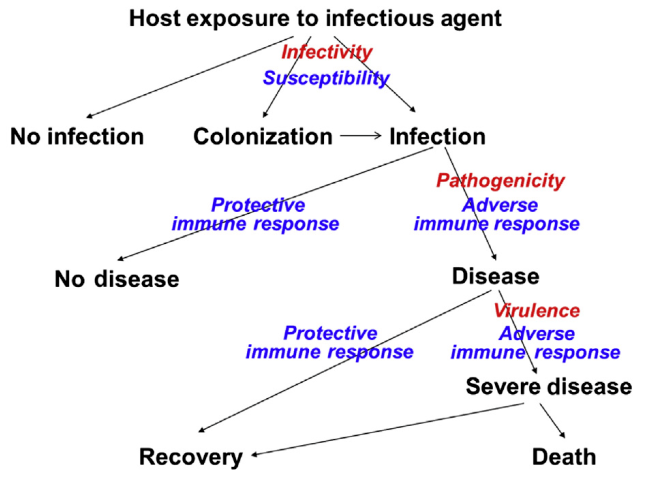
\includegraphics[width=.5\textwidth]{2 - Modelling of infectious diseases/fig/infectious_disease_outcomes.png}
    \caption{Potential outcomes of a host exposed to a pathogen (infectious agent) with depending factors of progression between stages. Figure copied from \cite{book:principles_infectious_diseases}.}
    \label{fig:infectious_disease_outcomes}
\end{figure}

\section{Concepts of infectious diseases}
\label{sec:concepts_of_infectious_diseases}
An infectious disease is an illness caused by any sort of pathogen, including bacteria and viruses, which is transferred from one host to another. Transmission of pathogens can occur in various ways, which is explained in Section \ref{subsec:transmission}, but does not necessarily mean that the new host will become ill. Figure \ref{fig:infectious_disease_outcomes} illustrates that exposure of a host to a pathogen can result in different outcomes. These outcomes are dependent on numerous factors such as the host's susceptibility to infection and disease, environmental factors, and physical and social behaviour of the host. If a new pathogen reaches a new host, it starts to colonize: multiplication of the pathogen at an entry point such as the skin or the mucous membranes of the respiratory, digestive, or urogenital tract. Then the pathogen starts to invade and establish within the host's tissue and causes disruption within a host, but does not necessarily result in disease. Clinical disease only occurs when a certain level of disruption has been reached which translates into symptoms and signs of illness. The final outcome of the disease varies in every situation, in which the immune system of the host plays a major role in. Depending on the host's immune system and the disease, the host may maintain immunity to the disease \cite{book:principles_infectious_diseases}.

\subsection{Transmission}
\label{subsec:transmission}
An important trait of many infectious diseases is that an infected host can act as a source of exposure to others. As will be explained in Chapter \ref{chapter:stride}, Stride focuses primarily on air-borne diseases such as measles, influenza, and COVID-19 which are mainly transmitted through means of direct contact. This thesis will thus concentrate on transmission through contact. For the sake of completeness however, we mention that there are five distinct means of transmission \cite{book:transmission_principles}:

\begin{enumerate}
    \item Through contact, direct (skin or sexual contact) or indirect (infected fomite, blood or body fluid). Inhaling contaminated air also falls into this category
    \item Ingesting contaminated food.
    \item Through vectors (mosquito, tick, etc.).
    \item Through pregnancy.
\end{enumerate}

\subsection{Stages}
\label{subsec:stages}
When a transmission of a pathogen has occurred, the exposed individual can become ill as discussed earlier. This does not mean that the recently infected person immediately becomes infectious to others or starts showing symptoms. Infectious diseases have different stages and the duration of those stages is different depending on the person and the type of infection, among other things. The time from exposure until the time of the first signs of symptoms of disease is called the \textit{incubation period}. After the incubation period, the \textit{period of clinical illness} starts which describes the duration between the first and last signs or symptoms. These periods are used to describe how the disease manifests itself to the infected person, but they do not say anything about the infectiousness of the infected person. The term to describe the time from exposure until the onset of infectiousness is the \textit{latent period}. The latent period is followed by the \textit{infectious period} which is the duration when the infected person can transmit pathogen. Figure \ref{fig:stages_infectious_diseases} visualises these periods for different types of diseases. It should be noted that these periods are an indication and that they can vary from person to person.  \cite{book:principles_infectious_diseases}
\\\\
The most obvious pattern of these stages is when the incubating and latent period are the same, as well as the clinical ill and infectious period. An example of such a disease is Ebola, and is shown in Figure \ref{subfig:stages_ebola}. Diseases where these patterns nicely follow up on each other are relative easy to treat and predict individually. Unfortunately there are also diseases where this is not the case.

\begin{figure}[!ht]
\centering
\begin{subfigure}[!ht]{\textwidth}
    \centering
    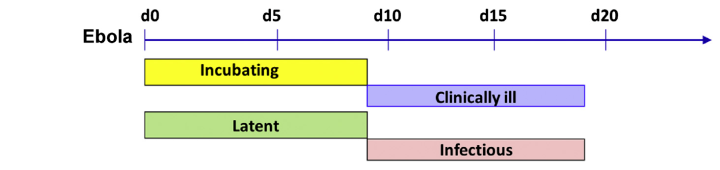
\includegraphics[width=.7\linewidth]{2 - Modelling of infectious diseases/fig/stages_ebola.png}
    \caption{}
    \label{subfig:stages_ebola} 
\end{subfigure}

\begin{subfigure}[!ht]{\textwidth}
    \centering
    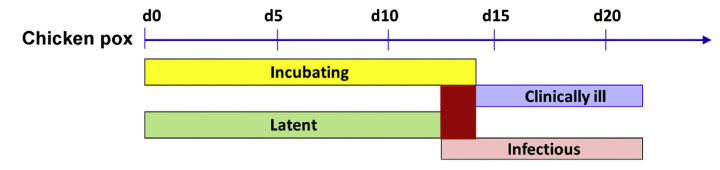
\includegraphics[width=.7\linewidth]{2 - Modelling of infectious diseases/fig/stages_chicken_pox.png}
    \caption{}
    \label{subfig:stages_chicken_pox}
\end{subfigure}

\begin{subfigure}[!ht]{\textwidth}
    \centering
    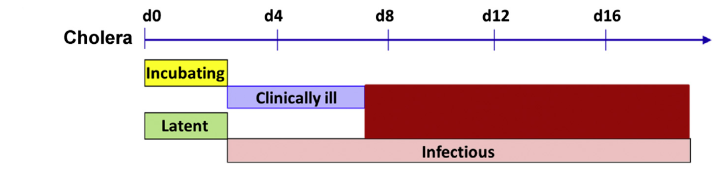
\includegraphics[width=.7\linewidth]{2 - Modelling of infectious diseases/fig/stages_cholera.png}
    \caption{}
    \label{subfig:stages_cholera}
\end{subfigure}

\begin{subfigure}[!ht]{\textwidth}
    \centering
    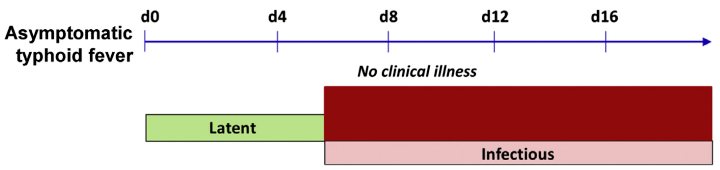
\includegraphics[width=.7\linewidth]{2 - Modelling of infectious diseases/fig/stages_asymptomatic_typhoid_fever.png}
    \caption{}
    \label{subfig:stages_asymptomatic_typhoid_fever}
\end{subfigure}

\caption[Stages of infectious diseases]{Stages of infectious diseases for different types of disease in function of the time since exposure (in days). The red bar displays when an infectious person is asymptomatic infectious. Figure copied from \cite{book:principles_infectious_diseases}.}
\label{fig:stages_infectious_diseases}
\end{figure}

\subsection{Asymptomatic carrier}
\label{subsec:asymptomatic_carrier}
It is possible that a person is infectious to others, but yet shows no signs or symptoms of disease. Someone who satisfies these conditions is called an \textit{asymptomatic carrier}, which can be divided in three different types of carrier \cite{book:principles_infectious_diseases}:
\begin{enumerate}
    \item \textbf{Incubatory:} This occurs when the incubation period overlaps with the infectious period and is for example the case with chicken pox, shown in Figure \ref{subfig:stages_chicken_pox}.
    \item \textbf{Convalescent:} In this case the clinically ill period ends before the infectious period. Cholera is such a disease and is visualised in Figure \ref{subfig:stages_cholera}.
    \item \textbf{Healthy:} This is the case when someone has no signs or symptoms, but still can infect others like with asymptomatic typhoid fever shown in Figure \ref{subfig:stages_asymptomatic_typhoid_fever}.
\end{enumerate}
It is clear that asymptomatic carriers make it harder to contain a disease. When treating infectious diseases it is therefore important to know when the different stages appear in order to take the appropriate actions such as contact tracing and isolation \cite{contact_tracing_and_disease_control}.

\subsection{Immunity}
\label{subsec:immunity}
Prevention of a disease can be more important than a cure, especially when trying to control an outbreak. Being immune to a disease therefore offers the best solution in prevention from getting ill. The actual workings of immunity will not be explained as they do not add value to this thesis. The different ways to become immune, however, deserve some elaboration to give insight in how this can effect the modelling of infectious diseases.
\\\\
The first case is called \textit{innate} immunity, which describes the immunity someone is born with \cite{innate_immunity}. The second case is \textit{adaptive} or \textit{acquired} immunity, and is used to denote the cases of immunity that are gained after being born. Once born, immunity can be acquired in four different ways as shown in Figure \ref{fig:immunity}. A distinction can be made between \textit{active} and \textit{passive}, and between \textit{natural} and \textit{artificial} immunity. Active immunity is gained when exposure to a pathogen triggers the immune system to produce antibodies for that pathogen, while passive immunity is gained when someone receives antibodies without being exposed to a pathogen. Active immunity can occur in a natural way when infected by a pathogen, or in an artificial manner when vaccinated. Likewise, passive immunity can happen in a natural way by receiving antibodies through breastfeeding or the placenta, or in an artificial way through globulin \cite{types_of_immunity}.

\begin{figure}[ht]
    \centering
    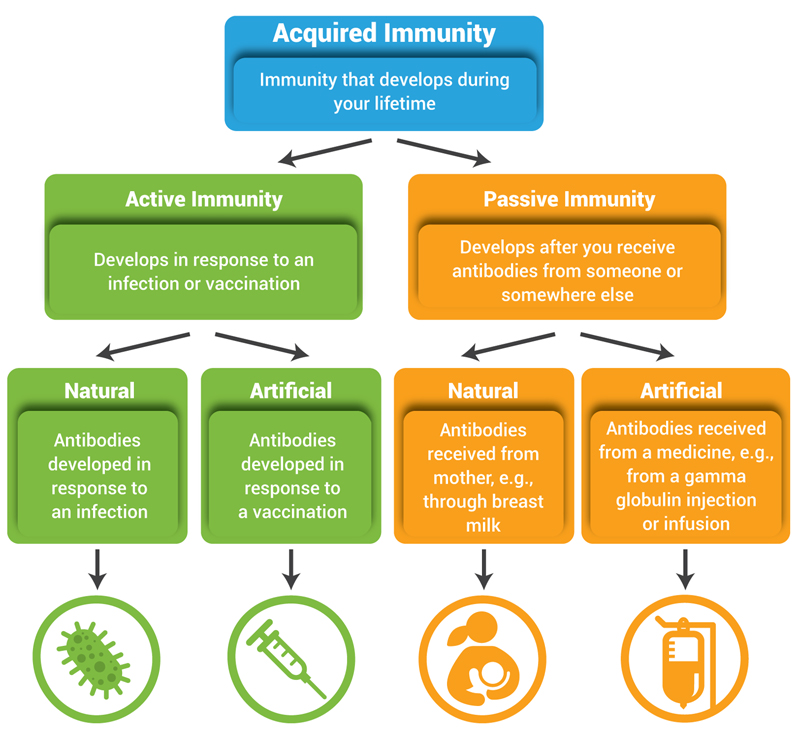
\includegraphics[width=.6\textwidth]{2 - Modelling of infectious diseases/fig/immunity.jpg}
    \caption{A visualization of the different types of acquired immunity. Figure copied from \cite{acquired_immunity}.}
    \label{fig:immunity}
\end{figure}

\subsection{Acute versus chronic}
\label{subsec:acute_vs_chronic}
The last thing that has to be discussed about infectious diseases is the different types of infection. The two most used terms to describe infections are \textit{acute} and \textit{chronic infections} and their key distinction is the duration of the infection. An acute infection lasts no more than six months, whilst a chronic infection lasts longer than six months. Also, the symptoms of acute infections develop rapidly over the course of days, in contrast to chronic infections where symptoms develop over weeks or months. Measles and influenza, the diseases Stride focuses on, are caused by acute infections. Therefore, whenever infectious diseases are mentioned in this thesis, they refer to those that are cause by acute infections \cite{acute_infections}.

\section{Mathematical models of infectious diseases}
A model is used as a representation of something and can be used by anyone in any field, with for example an architect who can build a scale model to represent their idea of a building. The architect's scale model can be just four walls and a roof, or the architect may have put incredible attention to detail in his work with by decorating every room. The difference in both models lies in the amount of work done by the architect. Likewise, a model to simulate infectious diseases can be a fast high-level program that produces little information, or a very complex program that needs a substantial amount of time to calculate detailed information of every individual. The next step in building such a model, is thus to understand how the recently gathered knowledge about infectious diseases can be applied and what trade-offs have to be made to get the desired results.

%\subsection{Basic reproduction number}
%Before moving on to the models, the basic reproduction number (denoted by $R_0$) needs a brief explanation. The number is a metric used to describe the contagiousness of a disease. Concretely, it represents the number of people that one infectious person will directly infect over the course of their infection, when placed in a fully susceptible population. \cite{r0}

\subsection{SIR model}
\label{subsec:sir_model}
Section \ref{subsec:acute_vs_chronic} explained that the focus lies on infectious diseases caused by acute infections, and thus the different stages of infectious diseases from Section \ref{subsec:stages} are short periods of time. Section \ref{subsec:transmission} also explained that the only type of transmission that will be considered is through contact. With this information, the most basic transmission model for a transmitted infectious disease can be used, called the SIR model which refers to its three compartments: susceptible, infected, and recovered. It is a system that consists of three coupled non-linear ordinary differential equations. The model makes use of very strict assumptions and is therefore not an abstract representation of the real world. There are numerous variations on the SIR model with different assumptions, but the basic assumptions are the following:
\begin{itemize}
    \item A large, fixed population represented as one large group, so without subgroups, where no demographic events occur.
    \item The infection has no latent period, thus an individual becomes infectious as soon as they become infected.
    \item Once someone is recovered, they are forever immune.
    \item Every person can encounter every other person with the same probability each day (which has nothing to do with probabilities, but rather with an intuitive model).
    \item The outbreak is normally short lived, but this can also be changed depending on the specified parameters.
\end{itemize}

\noindent Although the model makes strong assumptions, it still provides a lot of value. With simple calculus, a great deal of information can be extracted such as the reproductive number of the disease, the rate of recovery, and the rate of infection \cite{sir_model_origin}.

\subsection{SEIR model}
\label{subsec:seir_model}
An aspect of the SIR model is that there is no latent period. However, Sections \ref{subsec:stages} and \ref{subsec:asymptomatic_carrier} showed that the latent period is an important part of infectious diseases. In order for a model to give a more accurate representation of infectious diseases, it thus needs to take this period into account. The SEIR model is a refinement of the SIR model that fulfills this need by adding the \textit{exposed} state between the susceptible and infectious states. The exposed state represents the latent period when someone has been exposed to pathogen, but in which the amount of pathogen is too low in order for the host to infect others. Figure \ref{fig:seir-model} illustrates how the exposed state gives the SEIR model a more accurate representation of infectious diseases \cite{book:modelling}.

\begin{figure}[ht]
    \centering
    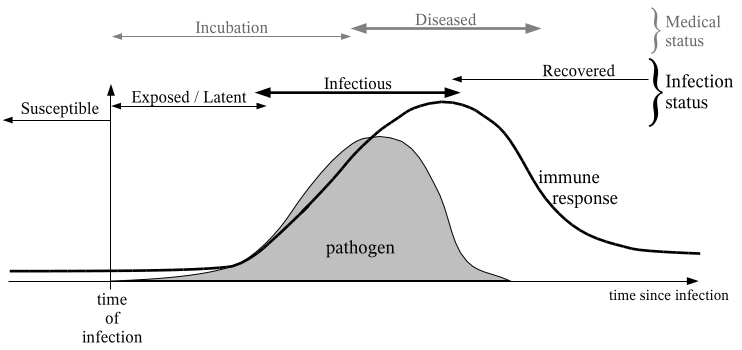
\includegraphics[width=\textwidth]{2 - Modelling of infectious diseases/fig/infection_timeline.png}
    \caption{A generalized representation of an infection over time, showing the different stages related to the dynamics of the pathogen and the host's immune response. Figure copied from \cite{book:modelling}.}
    \label{fig:seir-model}
\end{figure}

\subsection{Additional refinements}
The SEIR model is more advanced than the SIR model, but it is far from perfect. Section \ref{subsec:immunity} explained how immunity can be achieved in different ways. Further refinement of these models would thus be to incorporate the possibility of people being born with immunity. Since people do not necessarily become immune to a disease once they have recovered from it, another refinement would be to add the possibility of people becoming susceptible instead of immune after recovery. A third refinement could satisfy the lack of asymptomatic carriers, which is explained in Section \ref{subsec:asymptomatic_carrier}, by adding the possibility of people being an asymptomatic carrier \cite{book:modelling}.

\subsection{Deterministic and homogeneous}
\label{subsec:deterministic_and_homogeneous}
The models that have been explained could be seen as deterministic models. Given the same starting conditions, they would produce the same results every time. These models are limited to uniform and homogeneous populations, but still provide useful insights in infectious diseases \cite{usefulness_models}. However, their resemblance of the real world lacks the structure and stochasticity of every day life. In real life, people are divided in sub-populations such as their household, workplace, and school, where they meet different people every day. Every decision someone makes can have an impact on what their next decision will be or even what someone else their decisions will be. In order to simulate real life, different decision outcomes need to be taken into account. The simulation of such a decision can be seen as the collection of every possible outcome, for which every outcome has a probability that it will happen. This role of chance has a big impact when the number of infected people is relatively small or when considering a small (sub-)population \cite{stochastic_modelling}.

\section{Computational model simulations}
\label{sec:computational_model_simulations}
Every simulation serves a certain purpose, and so computational models can be designed in different ways to serve different purposes. This last section of the introductory chapter explains, based on Stride, how a computational model can be build to simulate infectious diseases. 

\subsection{Individual-based models}
\label{subsec:individual-based_models}
Section \ref{subsec:deterministic_and_homogeneous} explained how the mathematical models give a more high-level representation of infectious diseases in a population. One of their concepts is that they make use of homogeneous populations, which states that everyone in the population is and acts completely the same. Their results show the transmission dynamics based on the amount of people in every compartment (susceptible, infected and recovered), which only tells something on a population-level \cite{compartmental_model}. These results thus do not tell anything about the individuals that get infected or who someone has contacts with. If such more detailed results are required, a different model design is needed.
\\\\
These details cannot be gathered from a homogeneous population model, because everyone is then the same and no distinctions can be made. A heterogeneous population is needed which is when there are distinct individuals each with their own `life'. These distinctions can be made based on age, places they visit, people they meet, and so on. Every individual has thus their own identity and information that needs to be captured as well as the interactions with everyone else. A model that fulfills these needs is an individual-based model of which the definition is given by Willem et al. \cite{lander_lessons_decade, lander_phd}:
\begin{quoting}
"A computer simulation for the creation, disappearance and movement of a finite collection of interacting individuals or agents with unique attributes regarding spatial location, physiological traits and/or social behaviour."
\end{quoting}

In an individual-based model the population is designed in a bottom-up fashion. The population-level information is now the result of all the interactions between the individuals and their `behaviour' \cite{lander_lessons_decade}. Behaviour of individuals can also change based on for example different days of the week (weekday and weekend), or when feeling ill. It also allows for different environments to be created where every environment has its own type of behaviour \cite{introduction_agent-based_models}.

\begin{example}
\label{example:different_behaviour}
When at work, people interact very different than when they are at home. When at home, the contacts between people are closer than those at work. As such, individuals in different environments will `act' in different ways.
\end{example}

\noindent These environments also give the possibility to incorporate different stochastic interactions for each environment, which is very valuable when looking smaller populations as was stated in Section \ref{subsec:deterministic_and_homogeneous}.

\begin{example}
\label{example:different_stochasticity}
An infectious person has a much higher probability of infecting members of their household than colleagues at work.
\end{example}

Additionally, these models can give the option to track every individual in as much detail as desired. This gives the possibility to create a `history' for every individual as well as their network of contacts, thus providing new information in understanding different phenomena \cite{lander_lessons_decade}.
\\\\
Overall, as stated by Murphy et al. \cite{introduction_agent-based_models}, these models can be of use in countless situations to provide insights into the adaptation and function of systems. Another important asset of them is that they grant these insights when access to field data is dangerous, unavailable, or impossible to collect, with for example the COVID-19 pandemic that made collecting field data extremely difficult. Furthermore, research with individual-based models is a growing community, where open-source information and software play an important role. This, together with the increasing computational power, ensures future improvements in this field \cite{introduction_agent-based_models, abm_surging_tool}.

\subsection{Parameterization}
\label{subsec:parameterization}

Next to creating a model, parameters that are passed to the simulation need to be established. It is obvious that parameters can greatly impact the results of a simulation and thus definitely need to be chosen carefully:

\begin{example}
Looking back at Examples \ref{example:different_behaviour} and \ref{example:different_stochasticity}, the different probabilities in every environment need to be defined with actual values. If the probability that someone acquires an infection is slightly higher or lower, it can result in respectively more or less infected people in a simulation.
\end{example}

There are numerous ways to gather the required data with open-source data proving a valuable asset in these situations. In some cases it might be challenging, because certain interactions may not exist or still need some research \cite{abm_methods_and_techniques}. When parameters need to be estimated, there is a level of uncertainty that needs to be accounted for. Various techniques have been presented to give more accurate estimations on parameters \cite{lander_understand_models, parameter_importance_bilcke}, with a more relevant study about transmission model parameters for seasonal influenza by Willem et al. \cite{lander_estimating}. What parameters and data are being used in Stride, will be seen in the next chapter.

\chapter{Stride}
\label{chapter:stride}
This chapter describes the main subject of this thesis, which is the individual-based simulator for the transmission of infectious diseases or Stride for short. Before diving into pseudo code, we will explain the reasoning behind it and discuss the most important concepts. Furthermore, we lay out and examine its workings, as well as the data that is being used.

\section{Key aspects}
Before diving into the details and code of Stride, we need a better understanding of the model. This is gained by first figuring out what the most important concepts of Stride were when it was designed, followed by the two most important aspects, namely the individuals and the contact pools. Lastly, the configurations will be discussed since they determine how the model should be run.

\subsection{Core concepts}
Computer models have proven to provide valuable information in the spread of infectious diseases and what results of countermeasures can be \cite{modelling_importance}. The paper in which Stride is presented by Elise Kuylen et al. \cite{stride} states the following:
\begin{quoting}
"Several individual-based models for the transmission of infectious diseases, that take into account heterogeneous social mixing, have already been proposed, but only a few of these, such as FluTE \cite{flute} and FRED \cite{fred} are publicly available as open-source projects."
\end{quoting}
The way they describe Stride is as follows:
\begin{quoting}
"An open-source individual-based model for infectious disease transmission, which explicitly takes into account age, type of day and context when simulating social contacts."
\end{quoting}
Stride's main goal is thus to give a more accurate representation of transmission of infectious diseases by making the simulations resemble more closely to real life. The way Stride does this is by heavily focusing on the social contacts and the different aspects that influence these, since social contacts are crucial for infectious disease transmission \cite{stride}.

\subsubsection{Age}
\label{subsec:age}
The first key aspect of social contacts in Stride is age. The model works on a heterogeneous population in which every individual is different, including their age. In calculating the contacts between people, age has a big impact on who someone meets. Figure \ref{subfig:age_mixing_pattern} shows Stride's resulting age-mixing pattern, which is a representation of the different contact rates based on age. This may seem odd at first, but the explanation behind the results is that people are mainly mixing with people of the same age. The diagonal line between the bottom-left and upper-right corner represents the contact rates between people of the same age, which also has the highest contact rates in each row and column. The bottom left yellow area is the result of children having contact with their peers at school, which also goes for the yellow area in the middle that represents people meeting with their colleagues. It is thus clear that age is a major influential factor in who an individual meets.

\begin{figure}
    \centering
    \subcaptionbox{Age-mixing patterns in which yellow indicates high contact rates and red low contact rates.\label{subfig:age_mixing_pattern}}[.45\textwidth]{
        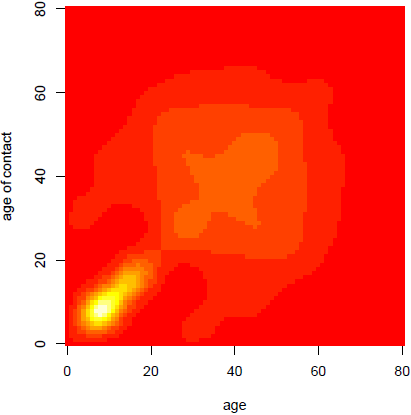
\includegraphics[width=.45\textwidth]{3 - Stride/fig/age-mixing_patterns.png}}
    \hfill
    \subcaptionbox{Number of influenza cases over time using different scenarios regarding the type of days.\label{subfig:type_of_day}}[.45\textwidth]{
        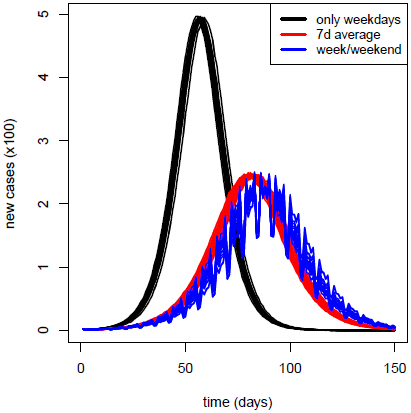
\includegraphics[width=.45\textwidth]{3 - Stride/fig/type_of_days.png}}
    \caption{Stride's social mixing results, copied from \cite{stride}.}
    \label{fig:stride_discussion_results}
\end{figure}

\subsubsection{Type of day}
\label{subsubsec:type_of_day}
Another important aspect Stride takes into account is the different type of days. A simulation in which every day is an average day, differs from more detailed simulations. Stride allows therefore for different type of days to be played out, such as weekdays, weekend days, and holidays. That fact that this is an important feature is confirmed in Figure \ref{subfig:type_of_day}, where the total number of infected cases is much higher when using only weekdays instead of different types of days. Likewise, the peak of number of new cases happens a lot earlier when using only weekdays and is significantly higher.

\subsubsection{Social context}
\label{subsec:social_context}
The last major aspect is the context of a social contact. Just as the age and the type of day, this is yet another very intuitive social trait. The context of contacts in Stride is viewed as the places where people can meet. Generally speaking, when in a household, the network density is a lot higher than at work regardless of age. How Stride handles these different social contexts will become clear during this chapter.

\subsection{Individuals}
\label{subsec:individuals}
Since Stride is an individual-based model, the most important parts are the individuals. Each person is defined by its own characteristics such as their age and health. A person's health status is based on the SEIR model, which is discussed in Section \ref{subsec:seir_model}, and can be either susceptible, exposed, infectious, recovered or vaccinated/immunized. Section \ref{sec:concepts_of_infectious_diseases} explained how people can have different reactions on infections, hence it is a rather important feature for a model to take into account when emulating real life. Therefore, every person's health has its own durations for the different stages of infectious diseases from Section \ref{subsec:stages}. How, when, and where individuals can have contact with one another depends on the contact pools in which each person can be present.

\subsection{Contact pools}
\label{subsec:contact_pools}
A person can be a member of four different \textit{contact pools}. These pools represent the different contexts in which an individual can have contact with someone. People are only able to have contact with members of the same pool who are present at the same time. These types of pools are the household, school or workplace, and two communities. An overview of the pools of an individual is visualised in Figure \ref{fig:pools_overview}, which also shows the days when someone can be present in each pool. An important rule is that an individual can only be a part of one pool per pool type.

\begin{figure}[ht]
    \centering
    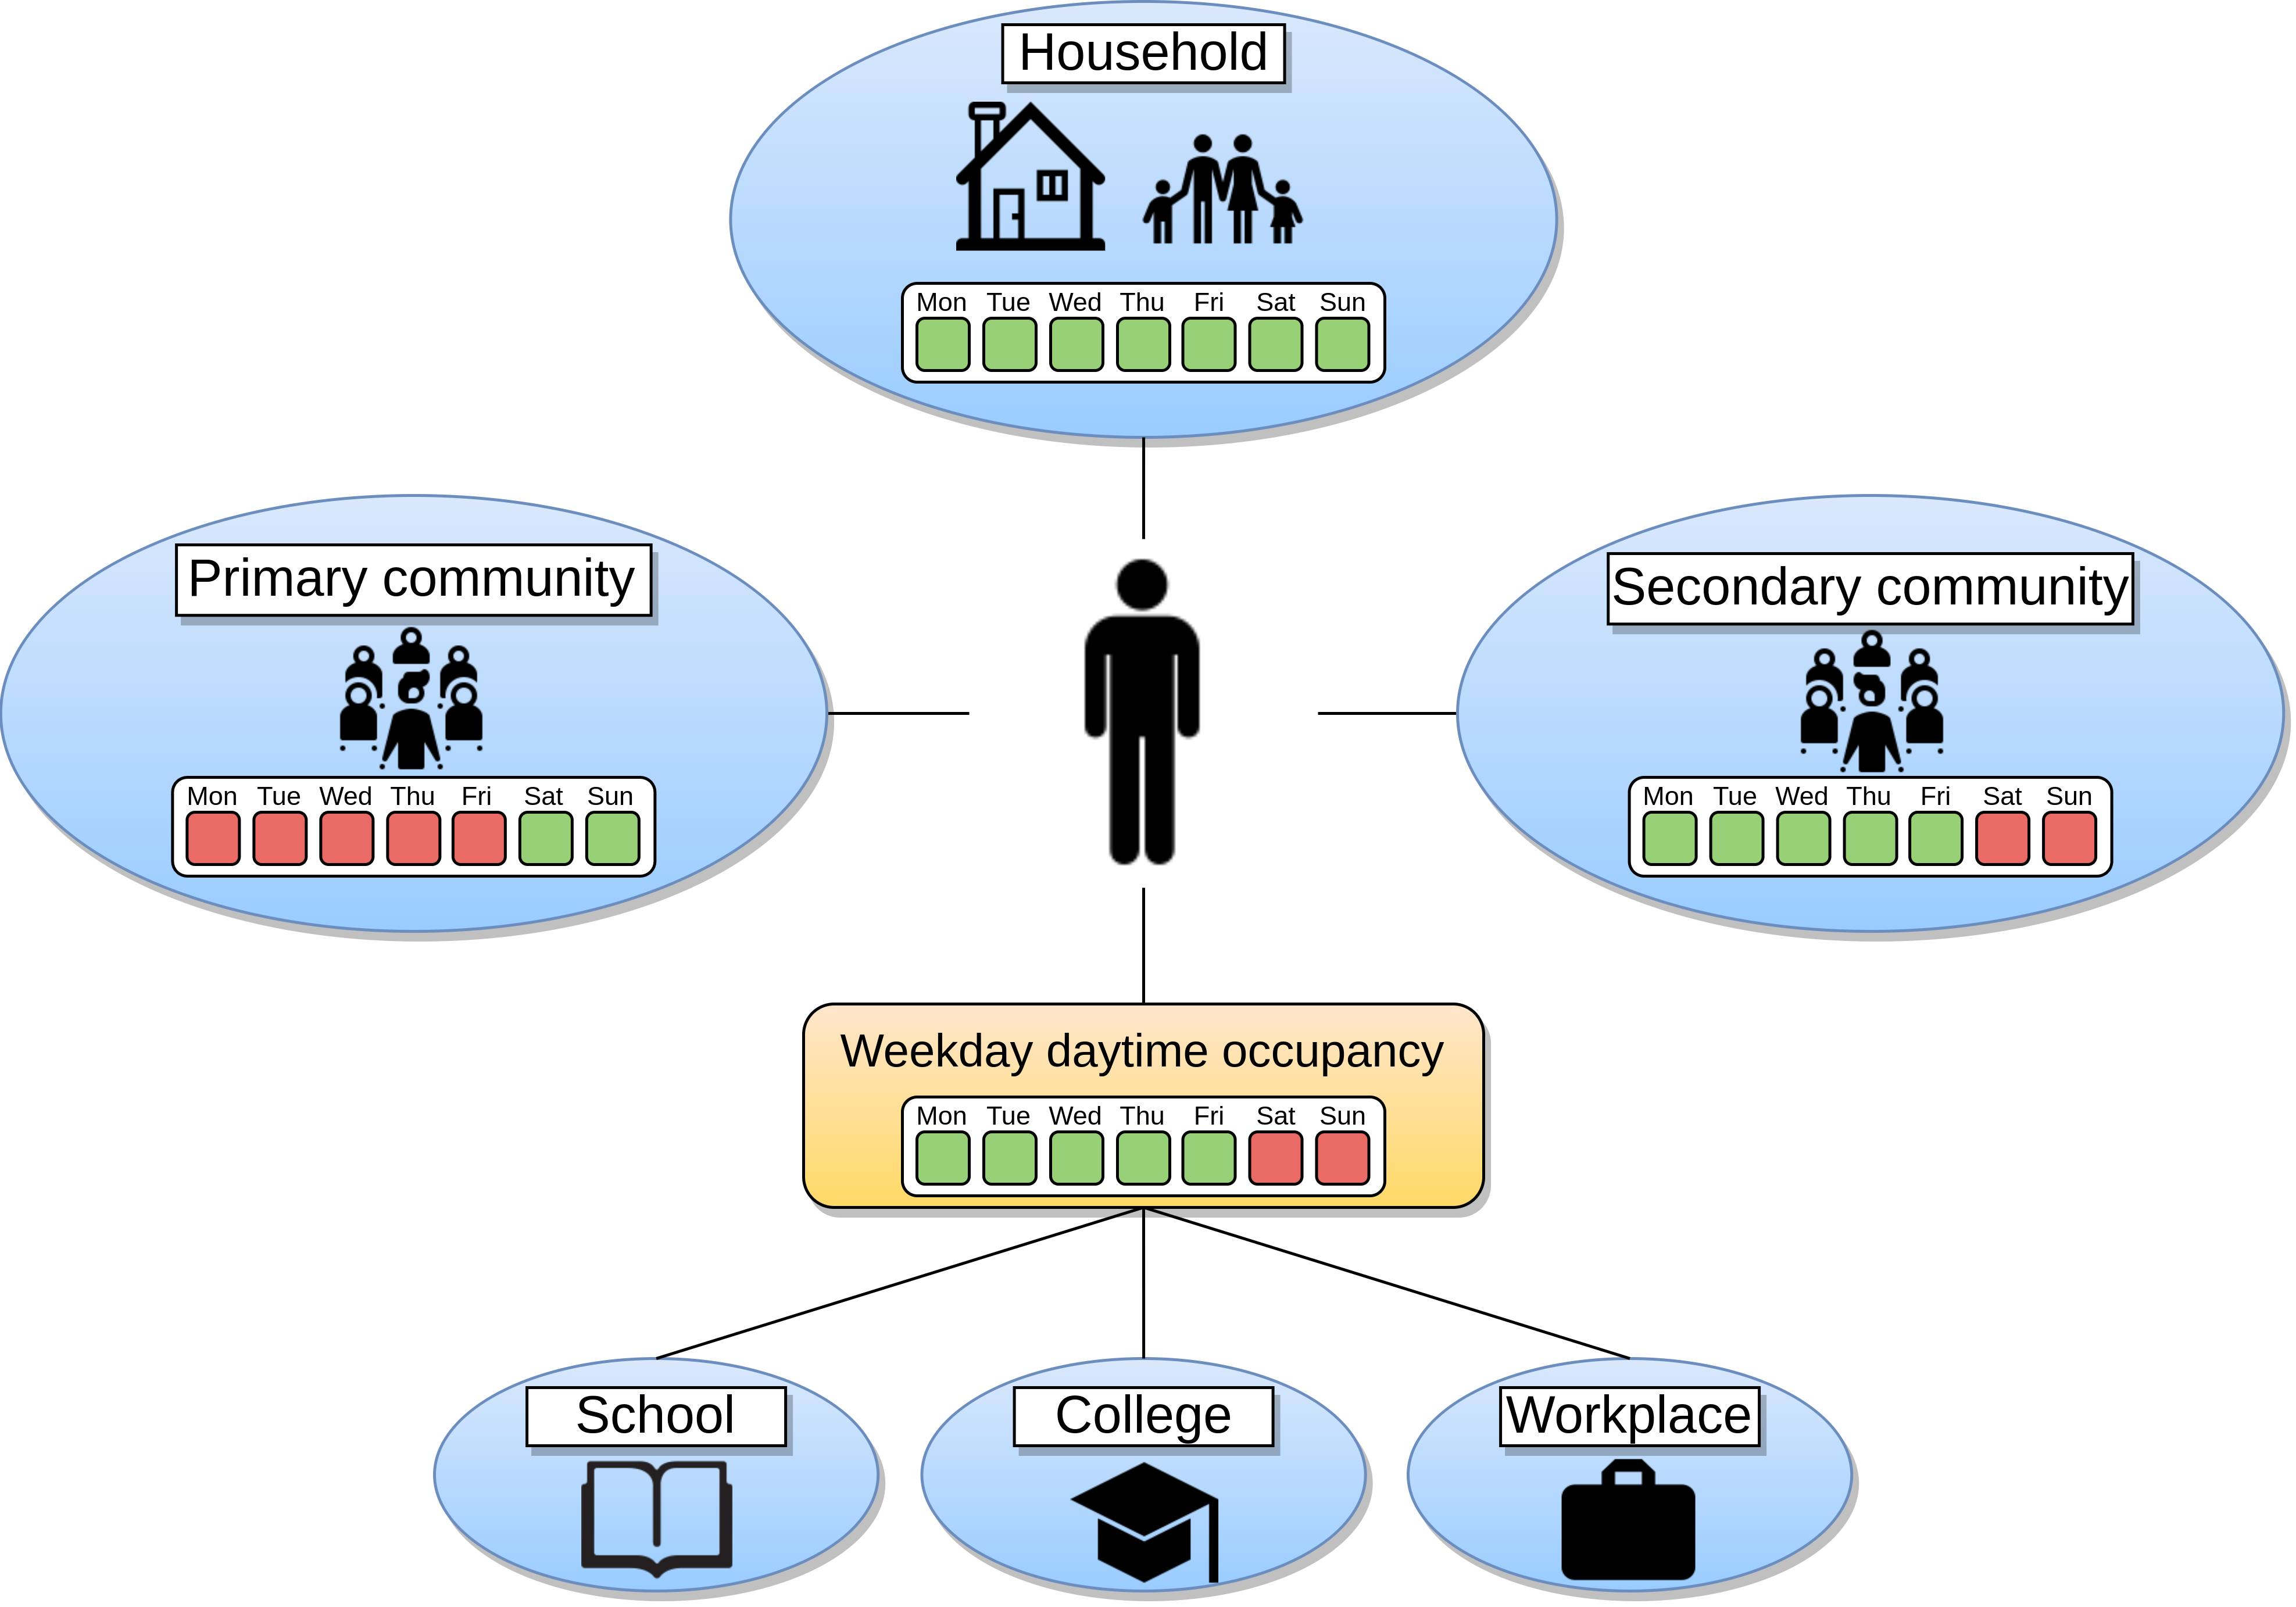
\includegraphics[width=\textwidth]{3 - Stride/fig/Pools_overview.png}
    \caption{Overview of the different type of contact pools. The days colored in green and red in each pool respectively show when an individual can be present or not.}
    \label{fig:pools_overview}
\end{figure}

\subsubsection{Household}
The most straightforward contact pool is the household. Everyone is a member of their own household and will be present in it every day of the week. There is however one exception to this rule, which is when someone is quarantined and is explained in more detail in Section \ref{subsec:pool_presences}.

\subsubsection{School and work}
Of the four types of pools someone can be a part of, there is one type which is not the same for everyone and that is the contact pool that represents an average individual's daytime occupation on a weekday. Just like in real life, what people do during a regular weekday is different for every person: children go to school and adults go to work. Following this logic, individuals younger than 18 years old should be a member of a school-pool and those 18 years and older of a work-pool. This might already be a solid representation for a model, but Stride makes a few extra distinctions here:
\begin{itemize}
    \item Children or young adults, which are people younger than 23 years old, do have a school contact pool, but these pools do not only consist of these people. Schools also need teachers who are of course adults. These teacher individuals are therefore not a part of a workplace contact pool, but instead of a school contact pool.
    \item Another distinction that can be made is the different types of school. This can be done in various ways, but Stride only separates K-12 schools and colleges. K-12 schools describe all the different types of education up until the age of 18 and colleges only contain (young) adults. Obviously, the school contact pools of the teachers and professors also make this distinction since they are in the same pool as their students.
    \item The workplace is the only pool of which an individual is not required to be a part of. A large part of the society in real life does not have a job or is retired. The individuals portraying these people are thus only a member of three contact pools.
\end{itemize}
The days when people can be present in their school or workplace pool are the weekdays from Monday to Friday, so weekend jobs do not exist in the simulation. However, as Section \ref{subsubsec:type_of_day} explained that Stride takes different types of days into consideration, the holidays cause for people to skip their school or workplace pools on these days. People who feel ill also typically don't go to school or their work, so they might then also not appear in their contact pool as will be seen in Section \ref{subsec:pool_presences}.

\subsubsection{Communities}
The last types of contact pools are the communities, of which there are two: the primary and secondary community. These pools represent the times when someone is not at school or work, and not at home. They can be described as the places and people someone meets in their spare time such as when practising a sport or other hobbies. Those pools represent the same concept, but do not occur at the same time or consist of the same people. The primary community is used for the contacts that are being made in the weekend and on holidays thus people can only be present in them on Saturday, Sunday and on holidays. Correspondingly, the secondary community represents the people someone can meet on a regular weekday outside of their school or workplace pool. Just as someone who feels ill will not go to school or work, they can also decide to stay at home and not attend their primary and secondary community.

\subsection{Configurations}
\label{subsec:configurations}
The previously mentioned aspects give more information about the model itself. How the model must be used in a simulation is decided by the various customisable configurations. Covering every single configuration would be a little otiose, so only the ones that are considered relevant will be explained.

\subsubsection{Population}
Sections \ref{subsec:individuals} and \ref{subsec:contact_pools} showed how individuals are being represented and how they are divided in contact pools where they can have contact with each other. These individuals and their contact pools are configured in a population file which contains a row for every individual. Such a row consists of non-negative integers representing the individual's age and the ID of every pool type as follows:
$$\textrm{(\textbf{age}, \textbf{household}, \textbf{school}, \textbf{work}, \textbf{primary\_community}, \textbf{secondary\_community})}$$
Since not everyone has to be a member of a school or workplace contact pool, it is possible for these values to be zero, indicating that they do not belong in one.

\subsubsection{Holidays}
As stated in Section \ref{subsubsec:type_of_day}, Stride makes a distinction between the type of days. Next to weekdays and weekend days, holidays are also being accounted for when deciding what kind of day the model has to simulate. These holidays are presented in a file that contains the information of all the days that have to be treated different than usual. This can be as detailed as needed and allows for distinctions to be made. There are for example days that are a national holiday and thus result in everyone not going to school or work (and their secondary community), but there are also holidays that only apply to schools such as summer break so that adults (not teachers) still need to go to work. Another similar example in Belgium is that colleges start somewhere mid September while K-12 schools start the first of September. In the holidays configuration file this is made possible by defining the ages to which a holiday applies.

\subsubsection{Disease characteristics}
Because the purpose of Stride is to enable the analysis of multiple infectious diseases, it needs a generic disease configuration file which describes the characteristics of the disease. This gives the possibility to simulate any disease on the basis of a couple traits. These traits consist of the basic reproduction number\footnote{Simplified explanation: the average number of people someone infects, which describes the infectiousness of a disease.}, the probabilities of being symptomatic or asymptomatic, how long someone can be infectious, etc.

\subsubsection{Event logging}
Subsequent sections will explain how Stride gives the possibility to run faster at the expense of generating less information. The main rule that defines this behaviour is the event logging rule. It determines what type of events need to be logged, such as the transmissions and contacts. The reason for this to have such an impact is that when contacts need to be logged, the model needs to evaluate every possible contact. If only transmissions need to be logged, it suffices to only calculate the transmissions instead of every possible contact. How this effects the model will become clear in Section \ref{subsec:contacts_and_transmissions}.

\subsubsection{Age contact matrix}
By now it is known how individuals and their contact pools are presented. These pools represent different social contexts in which people can have contact with each other. How people interact with one another in every pool is given by the age contact matrix file. This file contains a matrix with the probabilities of two people having contact with respect to their age and the pool type in which they find themselves in. Passing this matrix on to the simulation instead of defining the probabilities in the code, allows for flexible and customisable usage. The details of how this matrix is being used is described in Section \ref{subsec:contact_matrix}.

\subsubsection{Numerical values}
At last, there are various configuration values that are plain numerals. For example the number of days that the model has to simulate, the date at which the simulation has to start, or the number of infected and immune people at the start. There is also a possibility for multi-threading by configuring the number of threads that have to be used, which will be talked about further along this chapter.

\section{Simulation}
\label{sec:simulation}
The next step in gaining insight into Stride is to figure out the simulation. This section will thoroughly explain how the model works and every important part will be covered in detail. A conceptual overview of the simulation flow with its most important components is illustrated in Figure \ref{fig:simulation_flow}. Stride begins by initialising the simulation, which is explained in Section \ref{subsec:initialisation}. Then the simulation commences at the starting date, moving forward in discrete time-steps of one day until the configured number of days have been processed. All of these days consist of the same pattern which is the following:
\begin{enumerate}
    \item Update the health status of every individual (Section \ref{subsec:health_status_update}).
    \item While updating everyone's health, also determine in which pool they will be present (Section \ref{subsec:pool_presences}).
    \item There is a possibility to perform contact tracing if this is set to be active (Section \ref{subsec:contact_tracing}).
    \item Make calculations to determine who has contact with each other and who gets infected (Section \ref{subsec:contacts_and_transmissions}).
\end{enumerate}
There is an additional step, universal testing, which will not be talked about in this thesis, because it was added after the start of the thesis and thus has not been examined. This testing step is similar to the contact tracing step, which is a very small part of the simulation that comes right after the contact tracing step and, as will be discussed in Section \ref{subsec:performance}, is therefore insignificant.

\begin{figure}
    \centering
    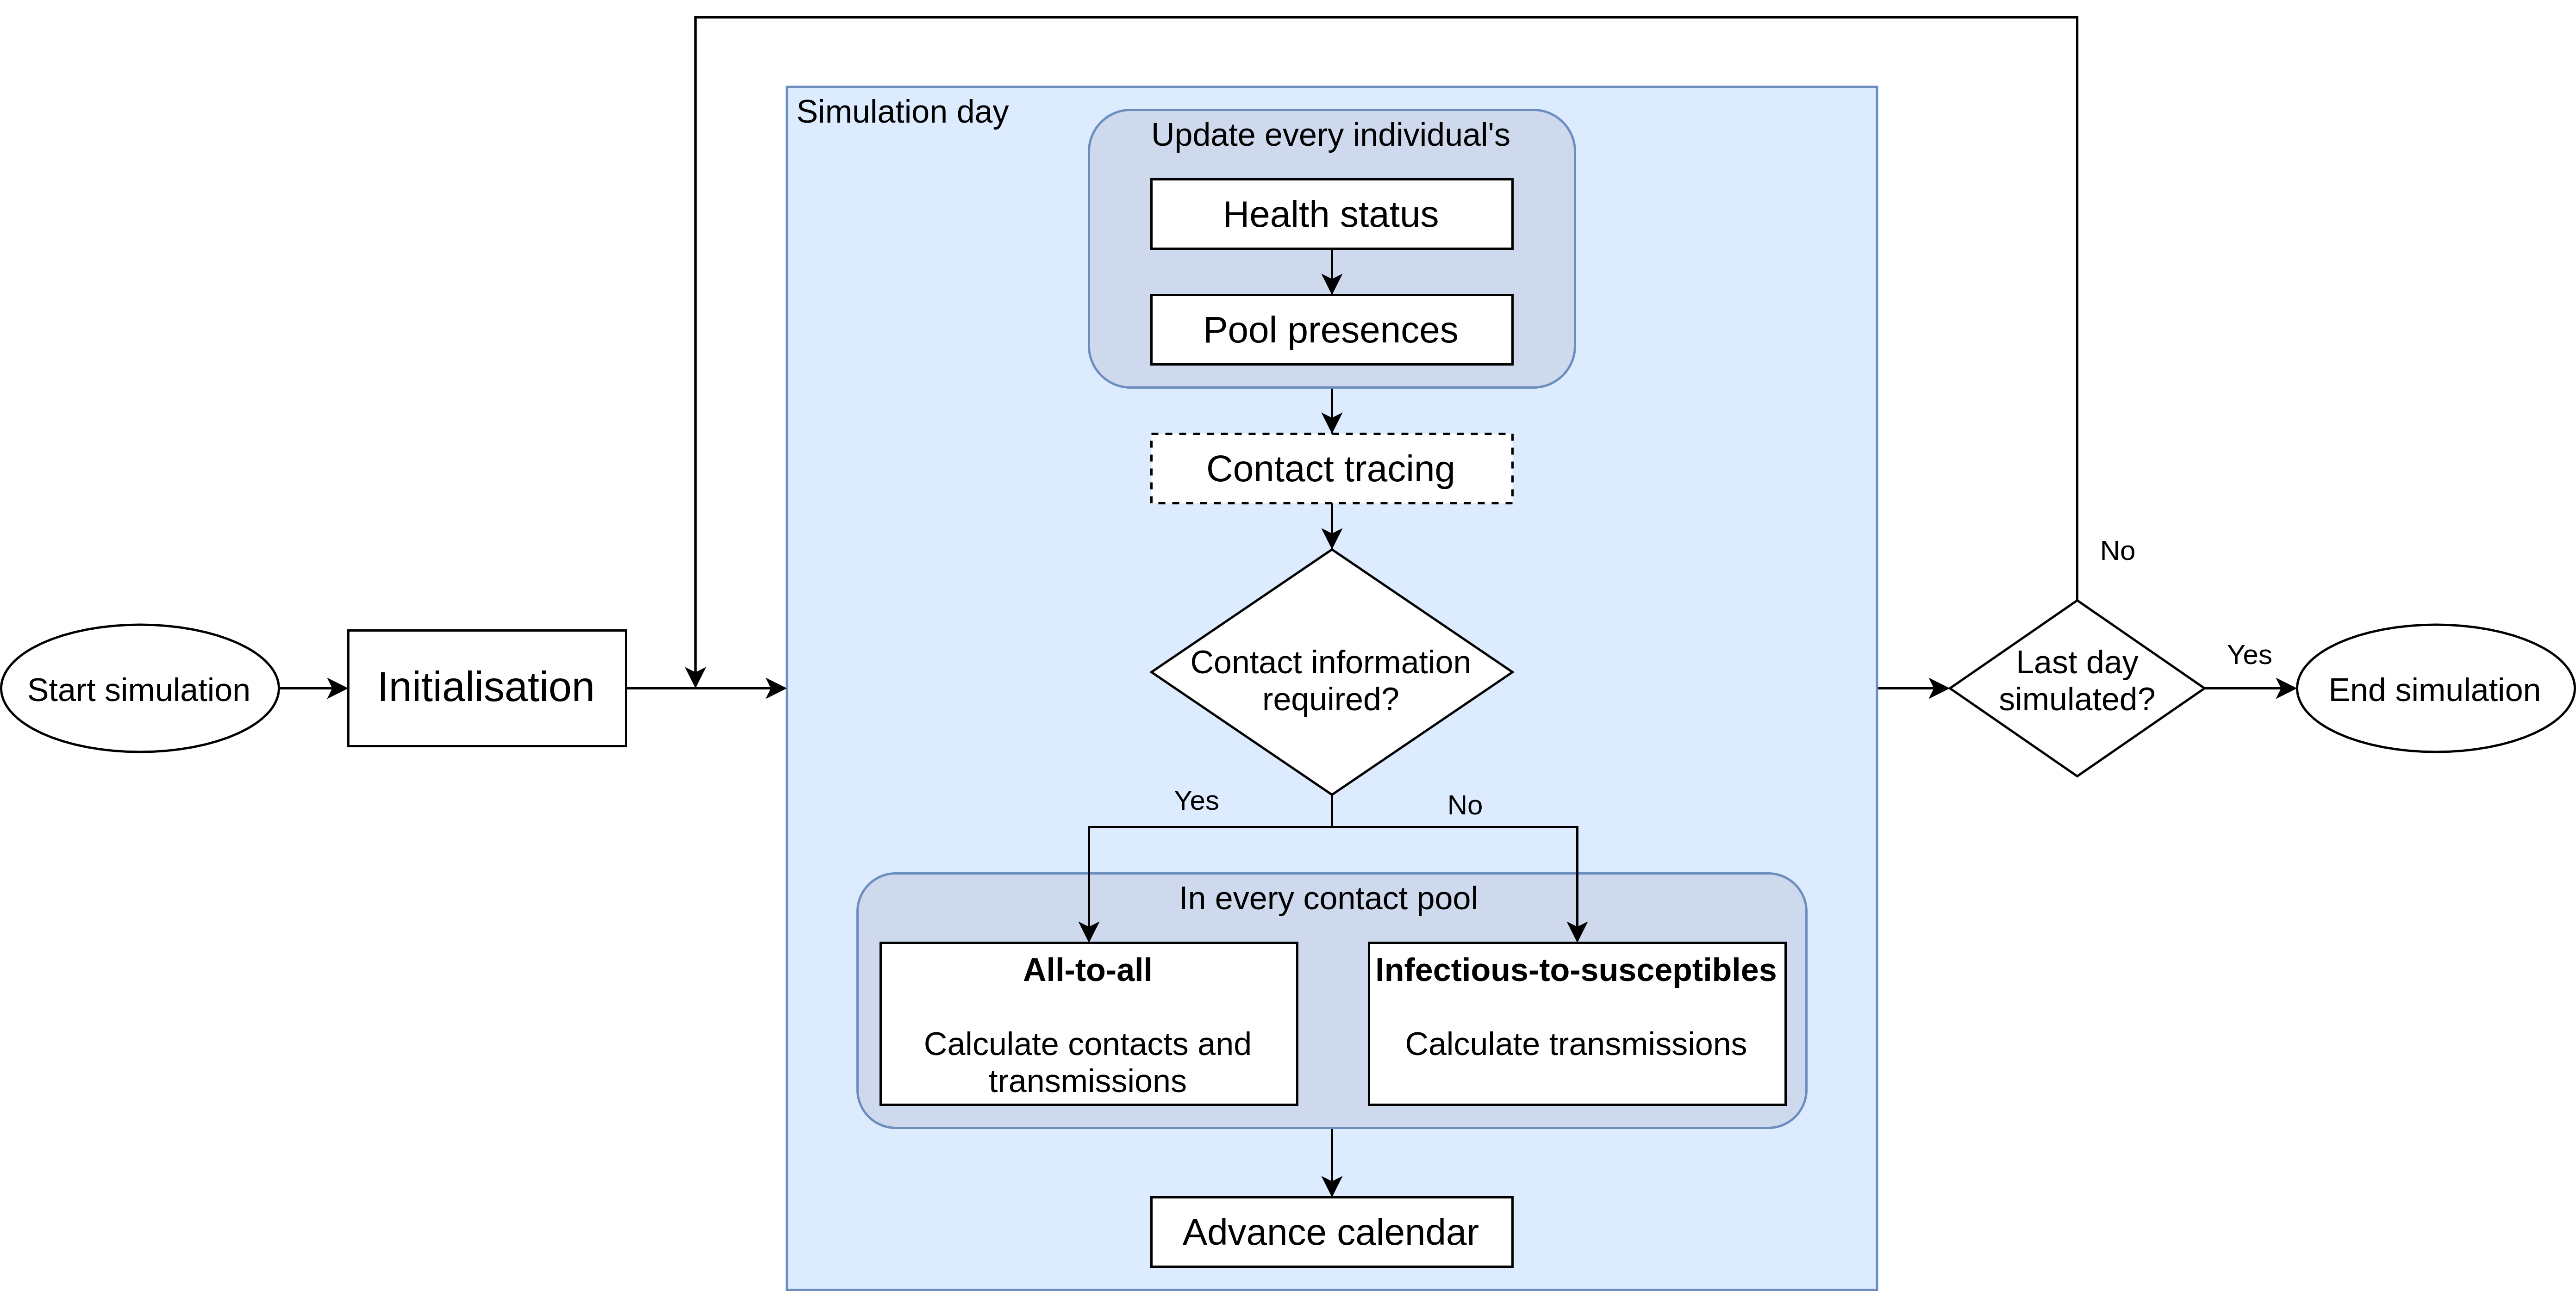
\includegraphics[width=\textwidth]{3 - Stride/fig/high-level_flow.png}
    \caption{Conceptual overview of a Stride simulation.}
    \label{fig:simulation_flow}
\end{figure}

\subsection{Initialisation}
\label{subsec:initialisation}
The initial step of the model is the initialisation, which uses the configurations from Section \ref{subsec:configurations} to set up all the necessary segments before starting the simulation. The first segment that gets initialised is the random number generator manager, which handles all the random numbers and distributions. Next is the population that gets created by generating every individual one by one from the population file, followed by the construction of all the contact pools. Then the calendar is built with the holidays file and the given start date, after which most of the numerical configuration values get processed. Thereafter are the contact matrix and disease characteristics read in and stored.
\\\\
The last step in the initialisation process is to `seed' all the random elements of the simulation. Individuals need to behave in different ways, not only regarding contacts, but also regarding the disease. Every individual's health therefore gets randomly created to determine how long the different stages of the disease will be, which are discussed in Section \ref{subsec:stages}, and whether they will be symptomatic or not. The other seeding that gets done is randomly selecting the individuals that will be infected or immune at the start of the simulation.

\subsection{Health status update}
\label{subsec:health_status_update}
When an individual has not been infected, this step is skipped because their health status does not change then. If someone is infected, however, the simulator will look at their health characteristics that were randomly assigned in the initialisation. On the basis of these characteristics, it determines how the person's health will be in the upcoming day. The different outcomes are that the person becomes or remains infectious, symptomatic, infectious and symptomatic, or that the infection stops.

\subsection{Pool presences}
\label{subsec:pool_presences}
We now know that individuals belong to a pool and can be present or not, but not how this is stored by our model. Every pool is represented by its unique Id, the contact pool type, and its members. It does not keep track of which members are present during the current day. If someone is present or not is only being stored by the person itself. Thus, after a person's health status is updated, their presence in every pool gets evaluated.
\\\\
There are various factors that affect in which pool someone will be present. The most straightforward one is what type of day the current day is, which can be a regular weekday, weekend day, or holiday. When a person is symptomatic and thus feels ill, there is a chance that they will not attend other contact pools except their household.
\\\\
Furthermore, there are factors which are not a part of the standard model, but they are additional features that can be passed on through the configurations. A possible feature is to close schools and workplaces to analyze how it reduces an outbreak. Another element that can be turned on is the ability for a person to work from home and the ability for the `government' of the population to enforce telework. The last non-standard factor is the possibility of quarantine, which translates in the person isolating themselves from every pool, with also being able to be isolated from their household and thus not be present in it.

\subsection{Contact tracing}
\label{subsec:contact_tracing}
If the configurations have indicated that on the current day there will not be contacts traced, then this step is skipped, which also goes for universal testing. For the sake of completeness, this step will only be briefly explained here, because it does not belong to the standard simulation flow. Even when it is incorporated in the simulation, it does not have a big impact on the run time as will be seen in Section \ref{subsec:performance}.
\\\\
The contact tracing step will iterate over the entire population and check who is infected and just recently `felt' symptoms in order to perform the contact tracing, because people who do not feel symptoms would normally not know they are infected. Infected individuals their contacts of the previous days have a probability that they will be traced, which can result in them being put into quarantine. This probability resembles the fact that people in real life do not perfectly know who they have been in contact with and is a numerical configuration value.

\subsection{Contacts and transmissions}
\label{subsec:contacts_and_transmissions}
The final and most important part of a simulated day is calculating every contact and transmission. This is done by iterating over the different pool types to see which pool is active on the current day, so for example the workplace, K-12 school, college, and secondary community contact pools get skipped when it is a national holiday. Then, all the pools of an active pool type are iterated over and get processed to determine the contacts and transmission. There are two algorithms that can be used to do these calculations, for which the choice is made at run time, depending on the need for information about contacts. If information about contacts is needed, the \textsc{All-to-All} algorithm will be selected. When the simulation only needs to handle transmissions and infections, the infectious-to-susceptibles algorithm is used.

\subsubsection{All-to-all}
The first algorithm, of which the pseudo code is shown in Algorithm \ref{alg:all-to-all}, matches everyone of a pool with each other and determines for each member pair if they will have contact and if someone infects the other. Since everyone gets compared with everyone, this algorithm will be called \textsc{All-to-All} from now on. For every member pair in a contact pool, of which both individuals are present, the probability that they have contact is calculated. Then we perform a Bernoulli trial to randomly determine if there is contact, which expresses two different outcomes, success (contact) and failure (no contact), given our contact probability. When contact has been made, the next step is to look at the health statuses of the pair. If one of them is infectious while the other is susceptible, the probability of transmission is calculated. Similar to determining contact, the incident of the infectious person transmitting the disease to the susceptible one is decided by a Bernoulli trial based on the transmission probability. The susceptible person then becomes infected by the infectious one.

\begin{algorithm}
\caption{Pseudo code of the \textsc{All-to-All} algorithm.}
\label{alg:all-to-all}
\begin{algorithmic}[1]
    \Require{$P_{1} \dots P_{N}$}\Comment{All members of the pool}\;
    \Statex
    \For{$i \gets 1$ to $N$}\Comment{Iterate over all members}
        \State $P_{1} \gets P[i]$
        \If{$P_{1}$ not present}
            \State continue to next $i$
        \EndIf
        \For{$j \gets i$ to $N$}\Comment{Iterate over members starting from $i$}
            \State $P_{2} \gets P[j]$
            \If{$P_{2}$ not present}
                \State continue to next $j$
            \EndIf
            \Statex
            \State $C_{prob} \gets$ probability $P_{1}$ and $P_{2}$ have contact
            \If{\Call{BernoulliTrial}{$C_{prob}$}}
                \State Register contact
                \If{$P_{1}$ or $P_{2}$ susceptible and other infectious}
                    \State $T_{prob} \gets$ probability infection happens
                    \If{\Call{BernoulliTrial}{$T_{prob}$}}
                        \State Infect the susceptible one
                    \EndIf
                \EndIf
            \EndIf
        \EndFor
    \EndFor
\end{algorithmic}
\end{algorithm}

\subsubsection{Infectious-to-susceptibles}
Section \ref{subsec:performance} will explain how the \textsc{All-to-All} algorithm becomes a lot slower depending on the number of people in a contact pool. Therefore, an optimised approach has been designed to be a lot quicker in exchange for producing less information. This other algorithm will be called the \textit{infectious-to-susceptibles} (\textsc{Inf-to-Sus} for short), because it only compares every infectious person in a pool with every susceptible one to determine who gets infected. At first, the pool gets sorted based on the health status of every member, which is explained in the next section, and it is counted how many infectious members the pool contains. If there are no infectious people in the pool, the algorithm immediately stops. However, if there are infectious members of the pool, the next step is to match the infectious ones with the susceptibles. For every pair of an infectious and a susceptible person, who are both present, the probability for them to have contact and the probability of transmission is calculated and multiplied with each other. This probability result is then used for a Bernoulli trial to randomly decide if the infectious person infects the susceptible one, after which the susceptible person becomes infected or not. Note that this algorithm only generates information about the transmissions and limits itself to contacts between infectious and susceptible persons. As such, it cannot be used to calculate contacts over the entire population, which the \textsc{All-to-All} method can.

\begin{algorithm}
\caption{Pseudo code of the \textsc{Inf-to-Sus} algorithm.}
\label{alg:inf-to-sus}
\begin{algorithmic}[1]
    \Require{$P_{1} \dots P_{N}$}\Comment{All members of the pool}\;
    \Statex
    \State sort $P[\;]$ on health status \Comment{Explained in Algorithm \ref{alg:health_sorting}}
    \Statex
    \State $N_{inf} \gets$ number of infected members
    \If{$N_{inf} = 0$}
        \State \Return
    \EndIf
    \Statex
    \State $i_{sus} \gets$ index of first susceptible member
    \State $i_{imm} \gets$ index of first immune member
    \Statex
    \For{$i \gets 1$ to $(i_{sus}-1)$}\Comment{Iterate over possible susceptibles}
        \State $P_{1} \gets P[i]$
        \If{$P_{1}$ not present or not infectious}
            \State continue to next $i$
        \EndIf
        \For{$j \gets i_{sus}$ to $(i_{imm}-1)$}\Comment{Iterate over susceptibles}
            \State $P_{2} \gets P[j]$
            \If{$P_{2}$ not present}
                \State continue to next $j$
            \EndIf
            \State $CT_{prob} \gets$ probability of contact AND transmission between $P_{1}$ and $P_{2}$
            \If{\Call{BernoulliTrial}{$CT_{prob}$}}
                \State $P_{1}$ infects $P_{2}$
            \EndIf
        \EndFor
    \EndFor
\end{algorithmic}
\end{algorithm}

\subsubsection{Sorting on health status}
Line 9 of Algorithm \ref{alg:inf-to-sus} may look like it performs a redundant check by confirming that \textit{p1} is infectious, but this is due to the way the contact pools are sorted on line 1. Algorithm \ref{alg:health_sorting} shows the pseudo code of this sortation based on the health statuses. A visual representation of a list of contact pool members before and after sorting on health statuses can be seen in Figure \ref{fig:health_sort}. Everyone who is immune is placed together at the end of the list and the susceptibles are arranged right in front of them. The remaining people with the health status exposed, infected, or recovered are put together with no specific order amongst them. \textsc{Inf-to-Sus} therefore needs to distinguish the infectious from the rest.

\begin{figure}
    \centering
    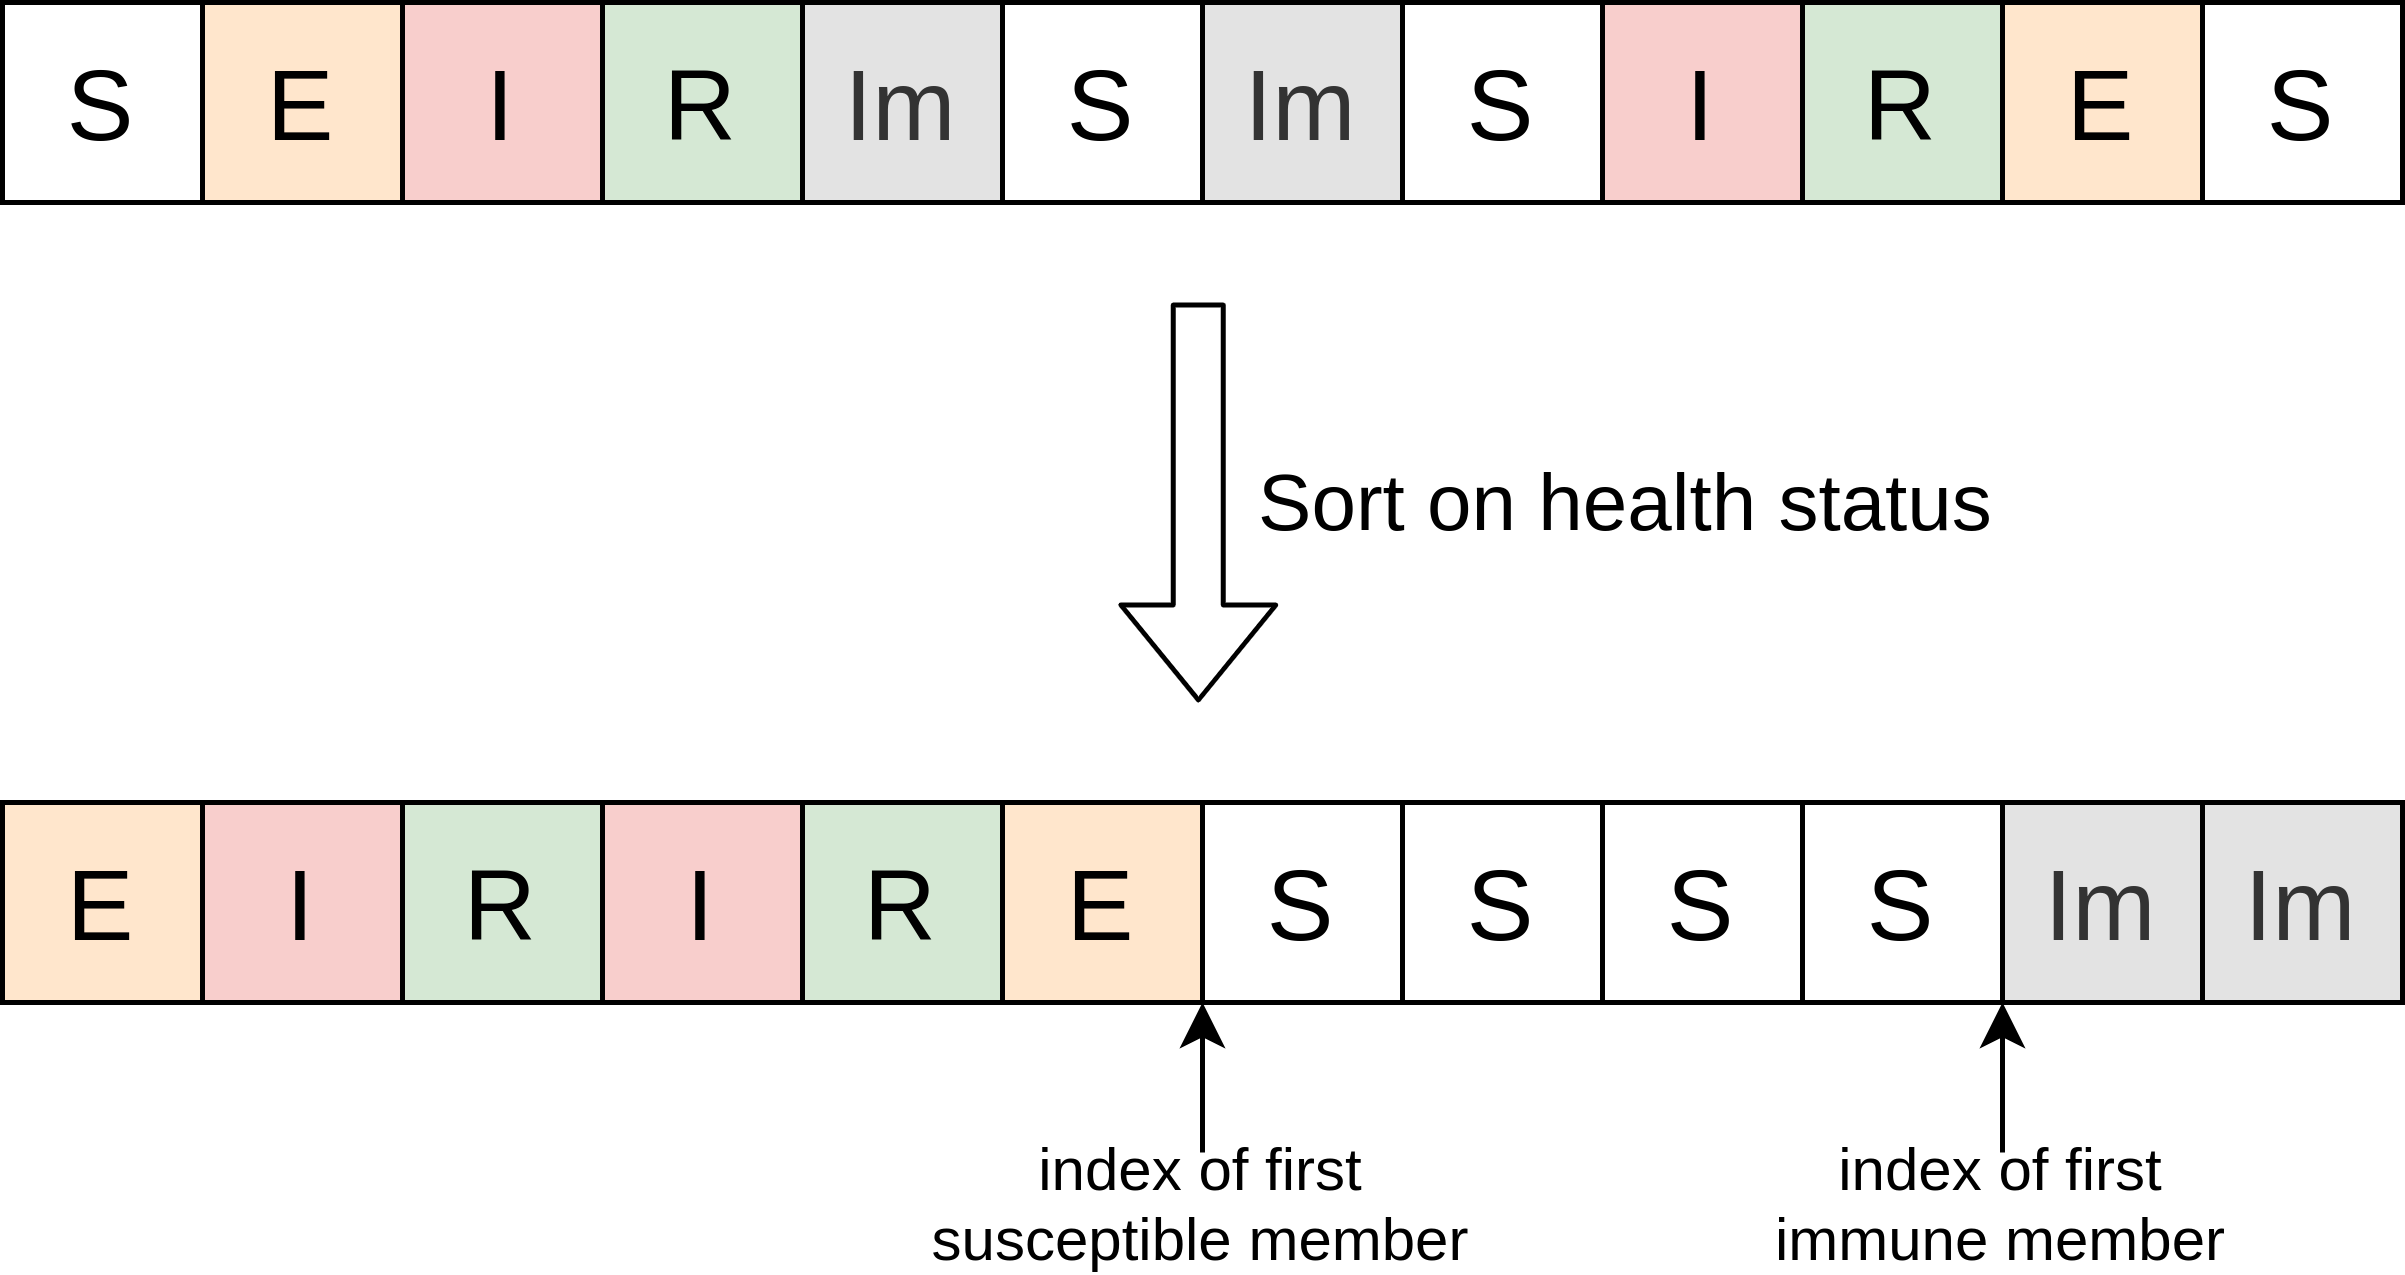
\includegraphics[width=.8\textwidth]{3 - Stride/fig/health_sort.png}
    \caption{Visual representation of a list of contact pool members before and after being sorted on health status, where every square represents a member. The letters indicate the health status of a member: Susceptible, Exposed, Infectious, Recovered, or Immune.}
    \label{fig:health_sort}
\end{figure}

\begin{algorithm}
\caption{Pseudo code of the function that sorts the members of a contact pool based on their health statuses.}
\label{alg:health_sorting}
\begin{algorithmic}[1]
    \Require{$P_{1} \dots P_{N}$, $i_{imm}$} \Comment{All members of the pool, index of first immune member}\;
    \Ensure{$P[\;] sorted$, $i_{imm}$, $i_{sus}$}
    \Statex
    \State $i_{sus} \gets 1$\Comment{Index of first susceptible member}
    \For{$i \gets 1$ to $i_{imm}$}\Comment{Iterate over the pool members}
        \State $member \gets P[i]$
        \If{member is immune}
            \State $i_{imm} \gets i_{imm}-1$
            \State $swapped \gets false$
            \While{$i_{imm} > i$ and not $swapped$}
                \State $member_{2} \gets P[i_{imm}]$
                \If{$member_{2}$ is immune}
                    \State $i_{imm} \gets i_{imm}-1$
                \Else
                    \State \Call{swap}{$member, member_{2}$}\Comment{Switch positions in $P[\;]$}
                    \State $swapped \gets true$
                \EndIf
            \EndWhile
        \Statex
        \ElsIf{member not susceptible}
            \If{$i_{sus} < i$}
                \State $member_{2} \gets P[i_{sus}]$
                \State \Call{swap}{$member, member_{2}$}\Comment{Switch positions in $P[\;]$}
            \EndIf
            \State $i_{sus} \gets i_{sus}+1$
        \EndIf
    \EndFor
    \State \Return $P[\;]$, $i_{imm}$, $i_{sus}$
\end{algorithmic}
\end{algorithm}

\subsubsection{Contact probability}
Calculating the probability that two people have contact with each other takes a lot of factors into account, so only an abstract explanation of this will be given here. The pseudo code of the function that does these calculations is given in Algorithm \ref{alg:contact_probability}. If the type of pool is a household, the contact probability is always $0.999$. Otherwise, the first step is to retrieve the contact rate for both individuals in the specific pool type, which is further explained in Section \ref{subsec:contact_matrix}. This number is a representation of how many contacts someone has in a specific pool type per day by looking at their age. These numbers are selected from the contact matrix, which is a configuration file, as seen in Section \ref{subsec:configurations}, based on the type of pool and the age of each individual. The lowest contact rate between the two individuals is then chosen as the definite number. This number is then multiplied by a contact adjustment factor based on the type of pool, which can be altered through the configurations. The adjustment factor is used, for example, to implement social distancing or intensify the contacts. The contact probability is then calculated by dividing these adjusted number of contacts by the total number of members in the pool minus one. This minus one represents a person themselves, with whom they of course cannot have contact with.

\begin{algorithm}
\caption{Pseudo code of the function that calculates the contact probability between two individuals in a contact pool.}
\label{alg:contact_probability}
\begin{algorithmic}[1]
    \Require{$P_{1}$,  $P_{2}$, $type$, and N}\Comment{Individuals, type of pool and total number of members}
    \Ensure{$prob$}\Comment{Probability of $P_{1}$ and $P_{2}$ having contact}
    \Statex
    \If{type = Household}
        \State \Return $0.999$
    \EndIf
    \Statex
    \State $contacts_{p1} \gets$ contact rate in pool($type$) for age($P_{1}$)
    \State $contacts_{p2} \gets$ contact rate in pool($type$) for age($P_{2}$)
    \State $contacts \gets min(contacts_{p1}, contacts_{p2})$
    \Statex
    \State  $factor \gets$ contact adjustment factor based on $type$
    \State $contacts \gets contacts * factor$
    \State $prob \gets contacts / (N-1)$
    \Statex
    \State $prob \gets min(prob, 0.999)$\Comment{Probability never higher than $0.999$}
    \State \Return $prob$
\end{algorithmic}
\end{algorithm}

\subsubsection{Transmission probability}
The probability of an infectious person transmitting their disease to a susceptible person when making contact depends on the combination of two things:
\begin{enumerate}
    \item The transmission probability of the disease itself, which is defined in the disease characteristics configurations.
    \item The relative transmission factor from the infected to the susceptible. This is based on a factor that represents the susceptibility if the susceptible person is younger than 18 years old, and the transmissibility if the infected is asymptomatic.
\end{enumerate}

\section{Data}
\label{sec:data}
Now that we have a better understanding of how our model works, we want to know what data it uses and how this data looks like. Because Stride can be run with different configurations and data, our goal here is not to focus on the data that has been used and examine it. Rather, we want to gain insight in the data that we will be using for the rest of this thesis, so that we can keep this knowledge in mind when analysing results. Eventually, our objective is to improve Stride in general, not just for a specific set of data.

\subsection{Population}
\label{subsec:population_data}
The first type of data we will look at is the population, for which Stride primarily uses the census data for Belgium from Eurostat\footnote{\url{https://ec.europa.eu/eurostat}}. For the research and tests of this thesis we used three different population representations, based on the 2011 census, which are also being used by the main researches of Stride: 600k, 3M, and 11M. These names are also an indication of the number of people every population contains, which is respectively 600 thousand, 3 million, and 11 million. 11M is the most accurate representation of the Belgian population and is naturally used for simulations regarding Belgium. 600k and 3M are smaller versions of the 11M which we only used when testing our optimisations. Therefore, we only discuss the 11M population in this section, of which the age distribution is shown in Figure \ref{fig:age_distribution}.

\begin{figure}
    \centering
    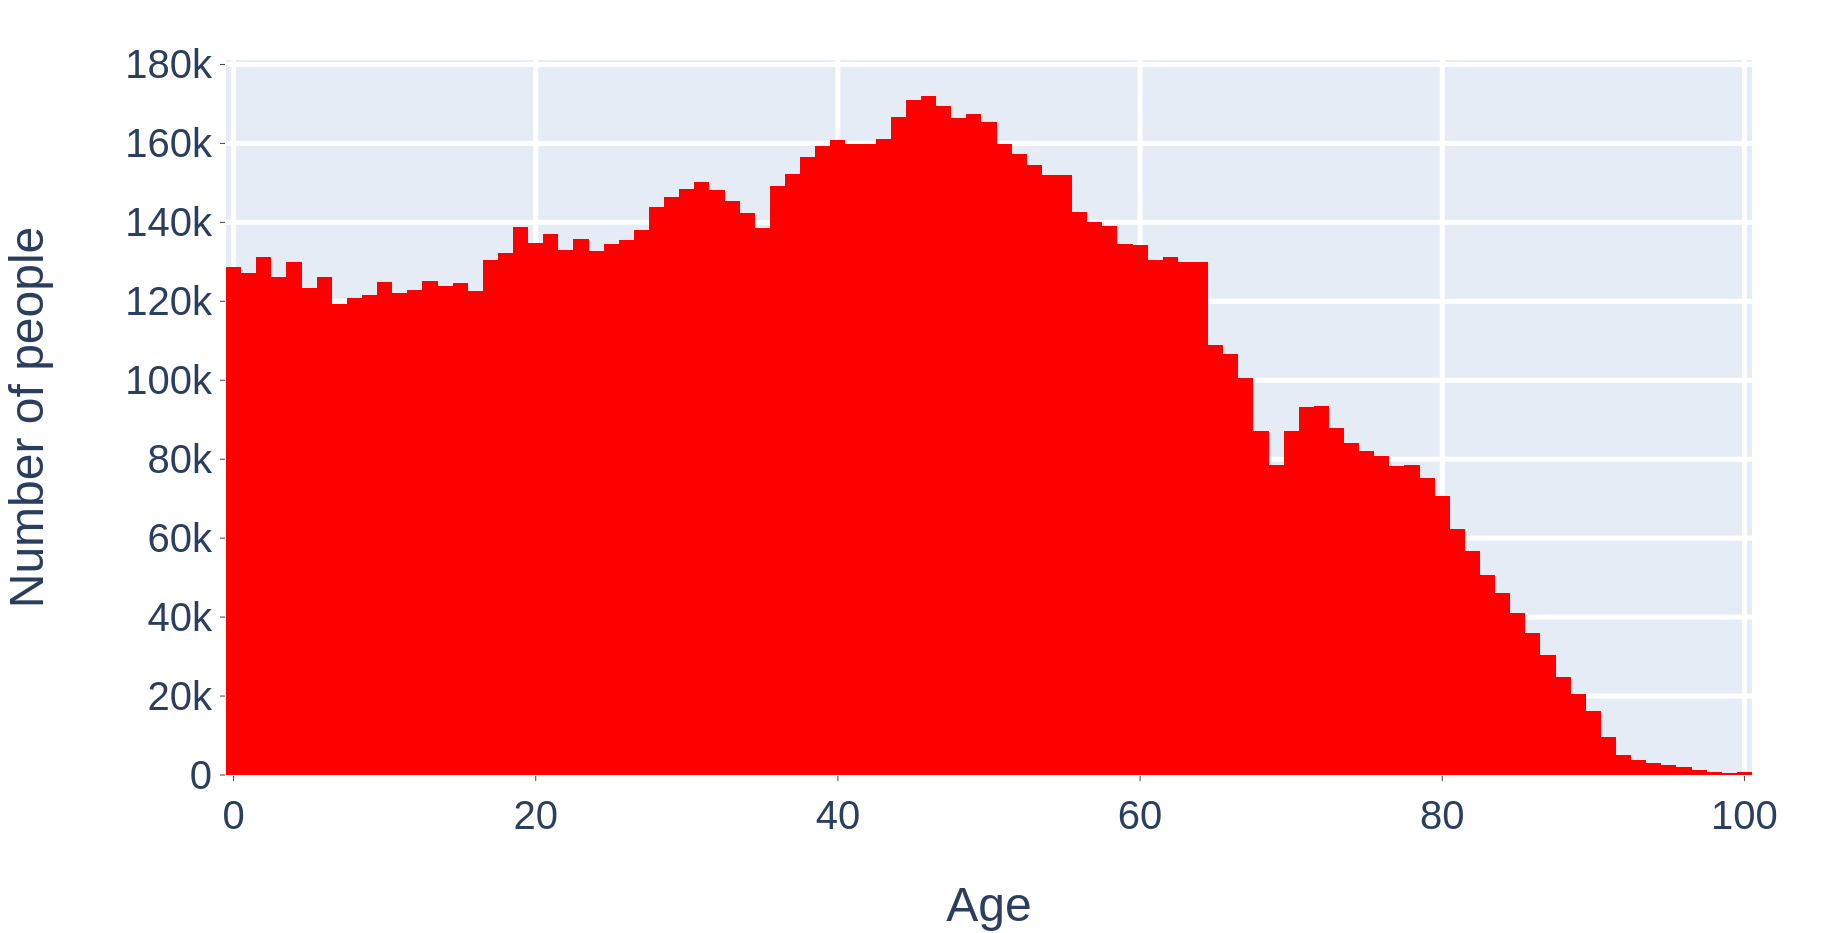
\includegraphics[width=.8\textwidth]{3 - Stride/fig/population_age_distribution.png}
    \caption{Age distribution of the 11M population.}
    \label{fig:age_distribution}
\end{figure}

\subsection{Contact pools}
\label{subsec:contact_pools_data}
All of the action in a Stride simulation occurs in the contact pools. This is where individuals have contact with one another and transmit the disease. Table \ref{tab:contact_pools_statistics} presents the general statistics of the different pool types next to each other. We see that there are vastly more household pools than any other type, but they are very small with a maximum of 6 and an average of 2.3 people per pool. The primary and secondary communities seem to be very similar and their average sizes are noticeably large. Workplaces can contain up to a thousand people, but are disproportionate compared to the other pool types with an average of 7.8 people. The school pools do not show any remarkable traits, but we will see that its general statistics are somewhat misleading. This information gives us a first view of the contact pools, however, a more profound analysis for every specific pool type is definitely needed.

\begin{table}
\centering
\resizebox{\textwidth}{!}{%
\begin{tabular}{@{}lrrrrr@{}}
\toprule
 &
  \multicolumn{1}{l}{Household} &
  \multicolumn{1}{l}{School} &
  \multicolumn{1}{l}{Workplace} &
  \multicolumn{1}{l}{\begin{tabular}[c]{@{}l@{}}Primary\\ community\end{tabular}} &
  \multicolumn{1}{l}{\begin{tabular}[c]{@{}l@{}}Secondary\\ community\end{tabular}} \\ \midrule
Number of pools & 4,859,837 & 131,756 & 566,759 & 22,000 & 22,000 \\
Min. pool size  & 1         & 6       & 1       & 51     & 44     \\
Max. pool size  & 6         & 50      & 1000    & 1431   & 1437   \\
Avg. pool size  & 2.3       & 20      & 7.8     & 500    & 500    \\ \bottomrule
\end{tabular}
}
\caption{General statistics of the contact pools of the 11M population.}
\label{tab:contact_pools_statistics}
\end{table}

\subsubsection{Household}
Since the total number of people in a household lies between one and six, there is probably not much variation possible amongst the household pools. Figure \ref{fig:household_poolsize_distribution}, which displays the distribution of household pool sizes, confirms this statement. 

\begin{figure}
    \centering
    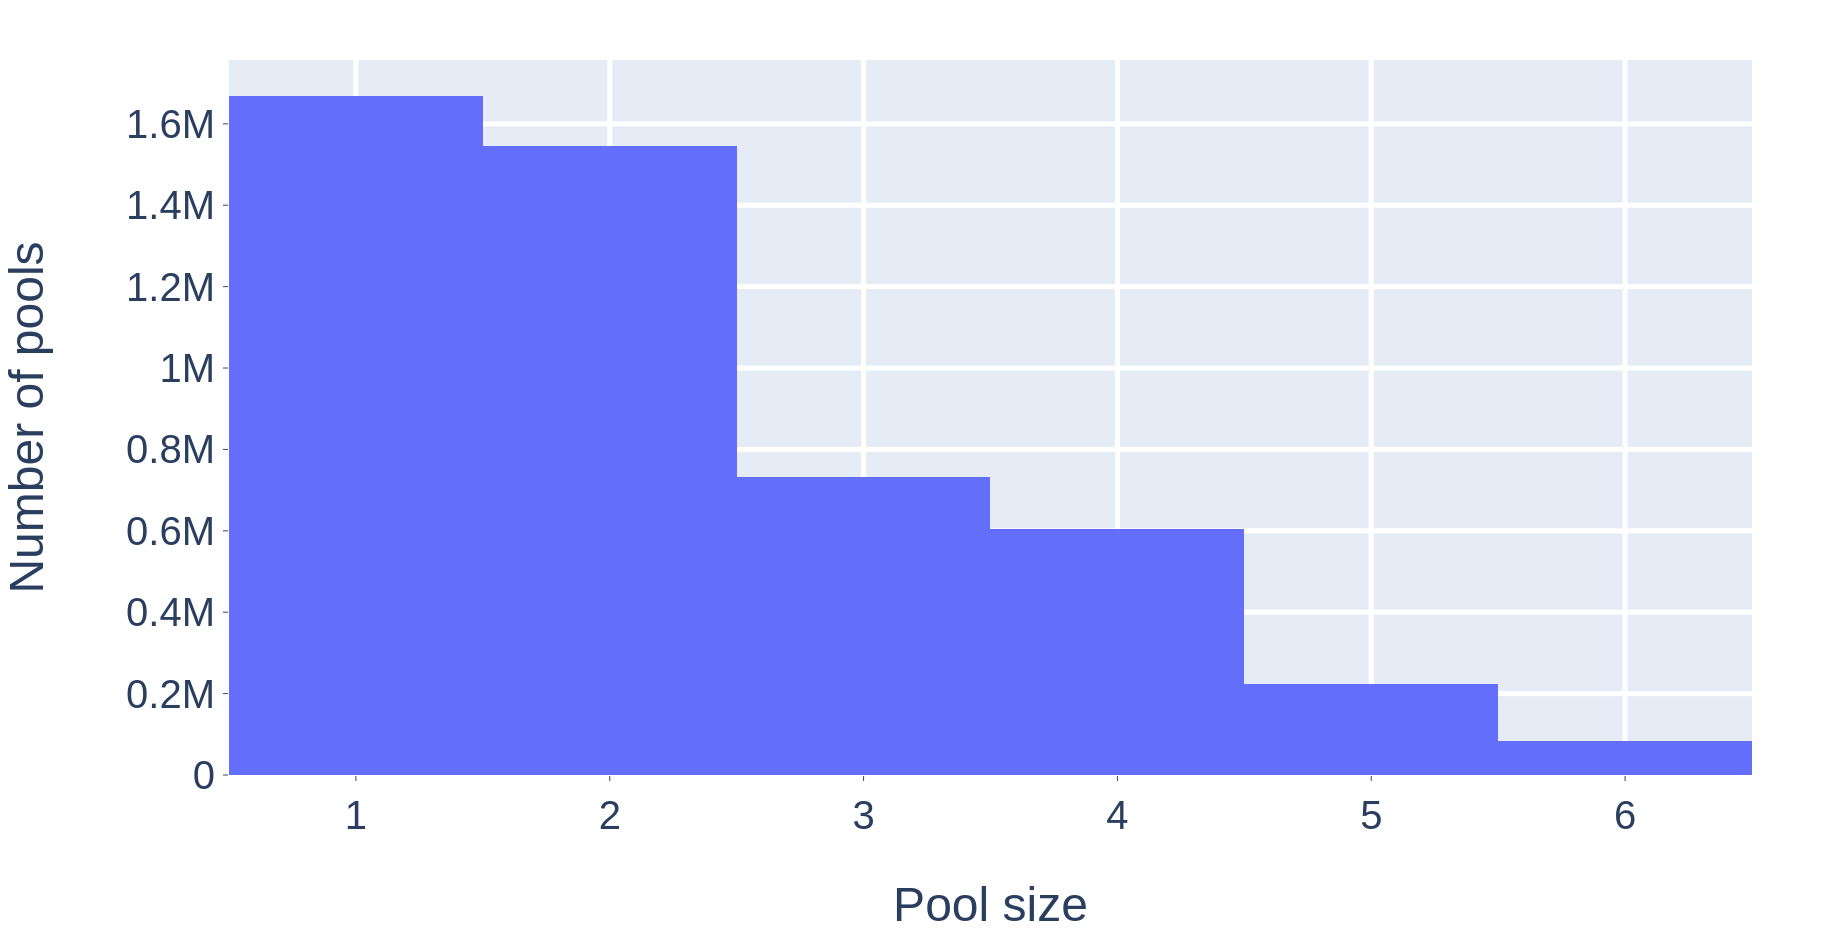
\includegraphics[width=.8\textwidth]{3 - Stride/fig/household_poolsizes.png}
    \caption{Distribution of the household pool sizes of the 11M population.}
    \label{fig:household_poolsize_distribution}
\end{figure}

\subsubsection{School}
Looking at the entire population, 24\% of the people have a school contact pool and only individuals younger than 60 years old can be a member, which Figure \ref{fig:school_age_distribution} shows us. In contrast with the general statistics, the distribution of school pool sizes in Figure \ref{fig:school_poolsize_distribution} shows that the school pool sizes are not evenly distributed and display a peculiar feature. We notice three different size `clusters': pools with size 1 to 10, 14 to 24, and 50. There is not much information that we can use from our 11M population to interpret these results, except for the age of the individuals in each cluster. Further inspection of the school contact pools with size 50 show that every individual is at least 18 years old. It is thus safe to assume that these only represent the college contact pools, which is also a logical explanation for the relative large pool sizes. The other two clusters do not show any age-specific traits, so we cannot say with certainty that these are only K-12 schools.

\begin{figure}
    \centering
    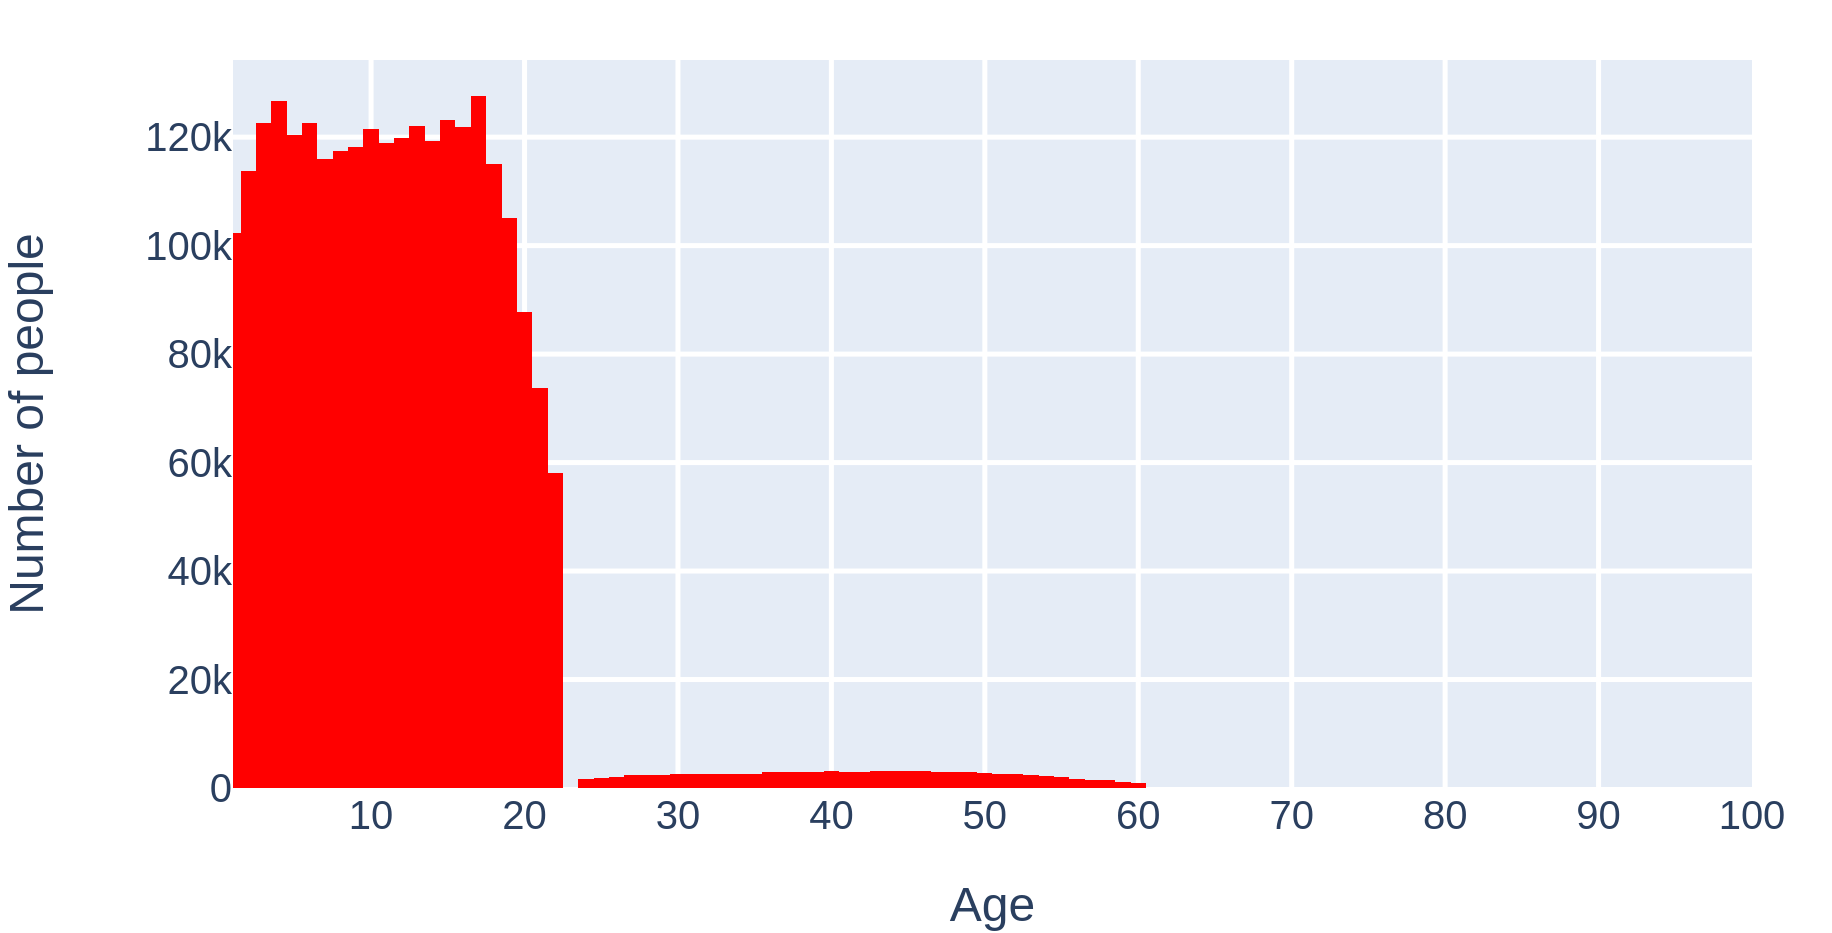
\includegraphics[width=.8\textwidth]{3 - Stride/fig/school_age_distribution.png}
    \caption{Age distribution of all the individuals that have a school contact pool in the 11M population.}
    \label{fig:school_age_distribution}
\end{figure}

\begin{figure}
    \centering
    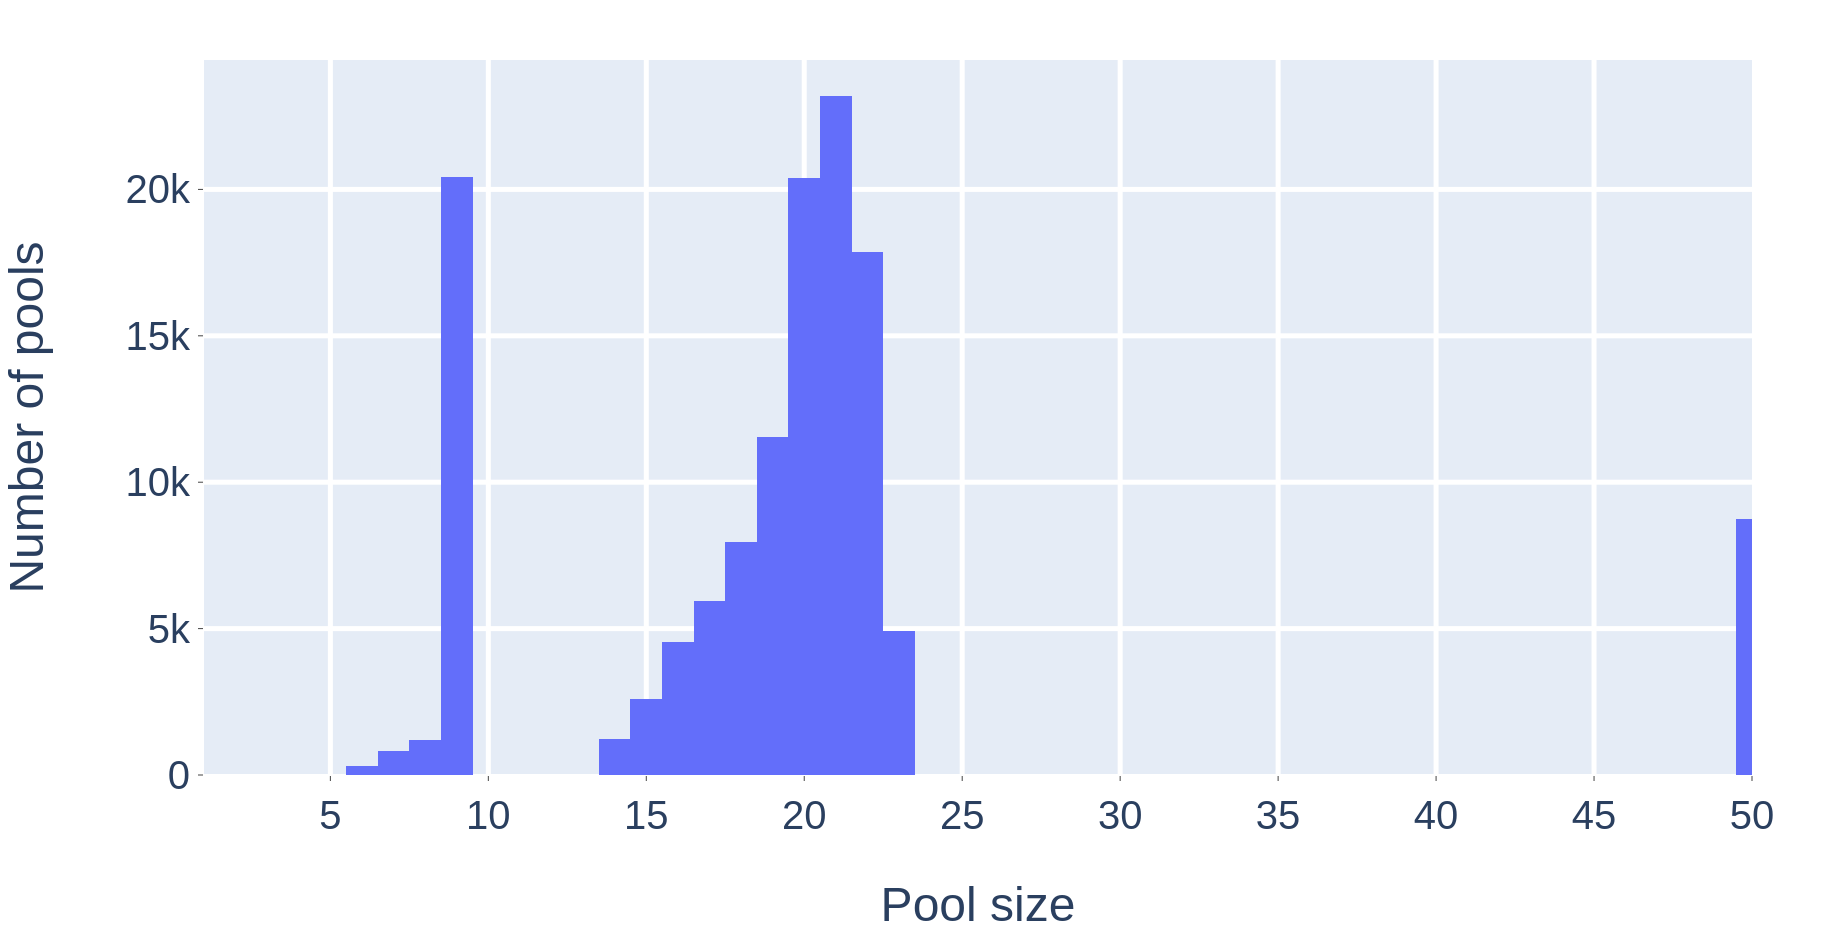
\includegraphics[width=.8\textwidth]{3 - Stride/fig/school_poolsizes.png}
    \caption{Distribution of the school pool sizes of the 11M population.}
    \label{fig:school_poolsize_distribution}
\end{figure}

\subsubsection{Workplace}
Just like with schools, not everyone has a workplace pool. 40\% of the population has a workplace contact pool and only people between the ages 17 to 77 can be a part of one, which is shown in Figure \ref{fig:workplace_age_distribution}. We also noticed how the workplace contact pools can contain one to a thousand people with an average size of 7.8. The distribution of workplace contact pool sizes displayed in Figure \ref{fig:workplace_all_poolsizes}, gives us insight into why this average size is so low. We clearly see that there is a major difference in the number of workplace pools with small sizes compared to the rest.
\\\\
In order to get a more detailed view of the number of workplace pools per size, we split them up in multiple age distribution ranges in Figure \ref{fig:workplace_poolsize_ranges}. The different ranges that we have chosen display more precisely the number of pools per pool size. We only notice that in Figure \ref{fig:workplace_10-50_poolsizes} there still is a big difference between the sizes smaller than 20 and the rest. Following this, we now look for `clusters' of pool sizes, or pool size ranges, in which the pool sizes in the same range have approximately the same number of pools. The ranges that we assume, looking at Figure \ref{fig:workplace_poolsize_ranges}, are: [1,9], [10,19], [20,49], [50,249], and [250,1000]. The statistics for these ranges in Table \ref{tab:workplace_stats}, confirm that our ranges contain pool sizes with similar number of pools. The range [1,9] contains, as expected, 94\% of all the workplace pools, but only consists of 60.5\% of the working individuals. So, although there are not that many workplace contact pools with more than nine people, they still account for 39.5\% of all the individuals with a workplace pool.

\begin{figure}
    \centering
    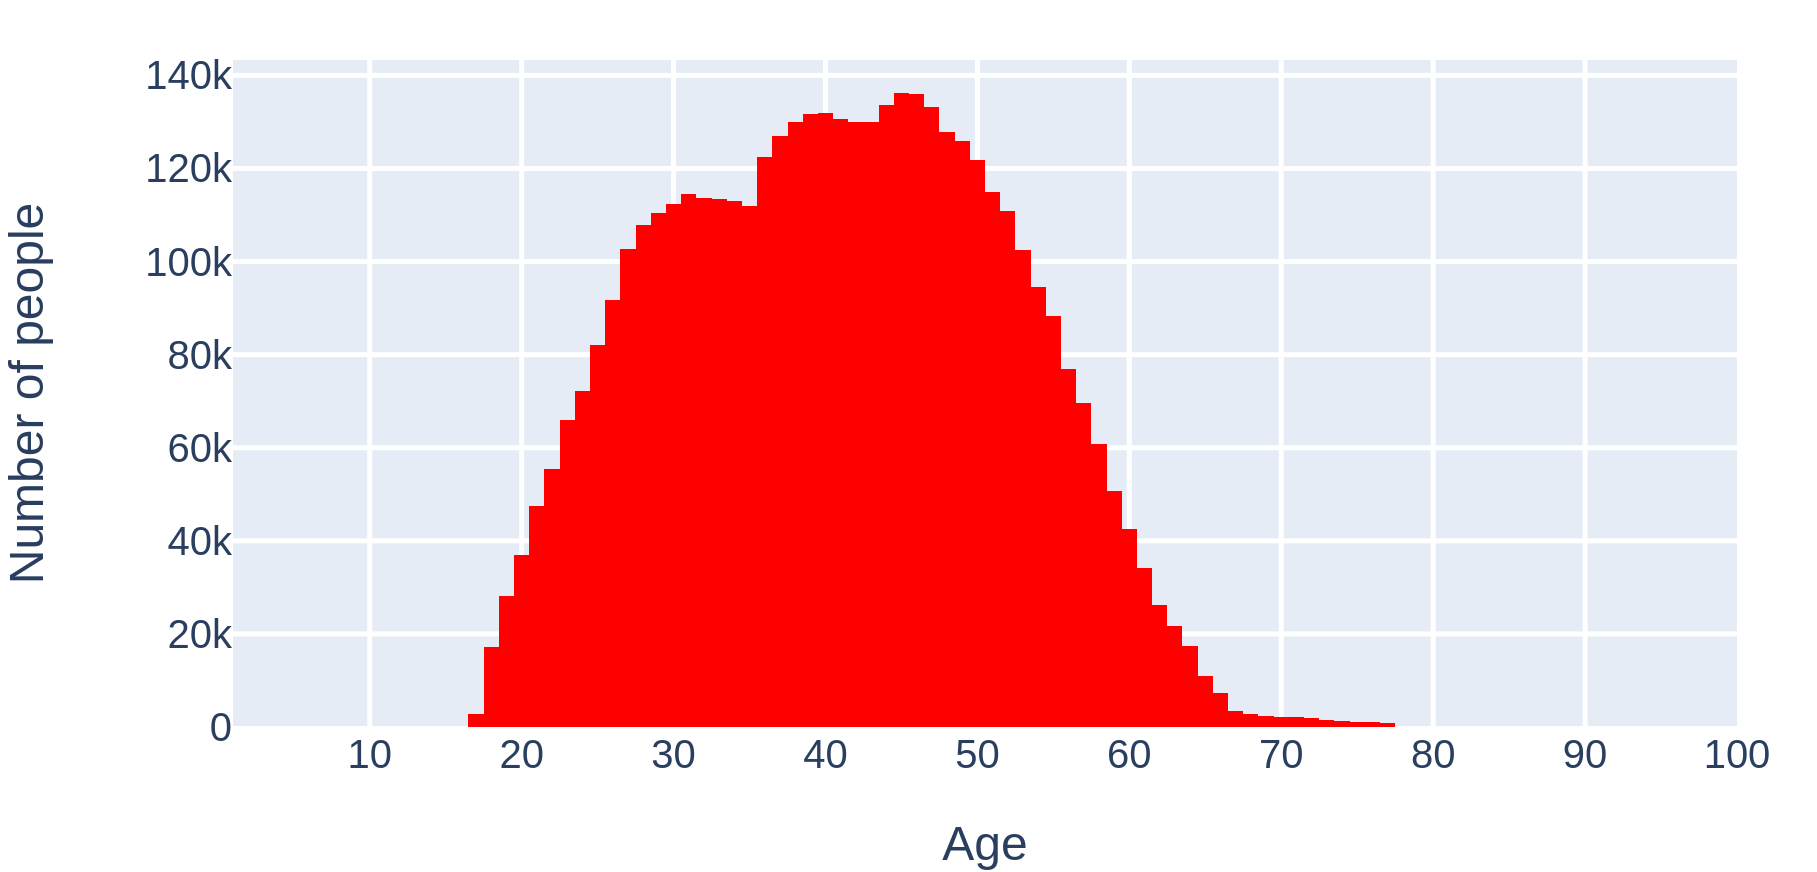
\includegraphics[width=.8\textwidth]{3 - Stride/fig/workplace_age_distribution.png}
    \caption{Age distribution of all the individuals that have a workplace contact pool in the 11M population.}
    \label{fig:workplace_age_distribution}
\end{figure}

\begin{figure}
    \centering
    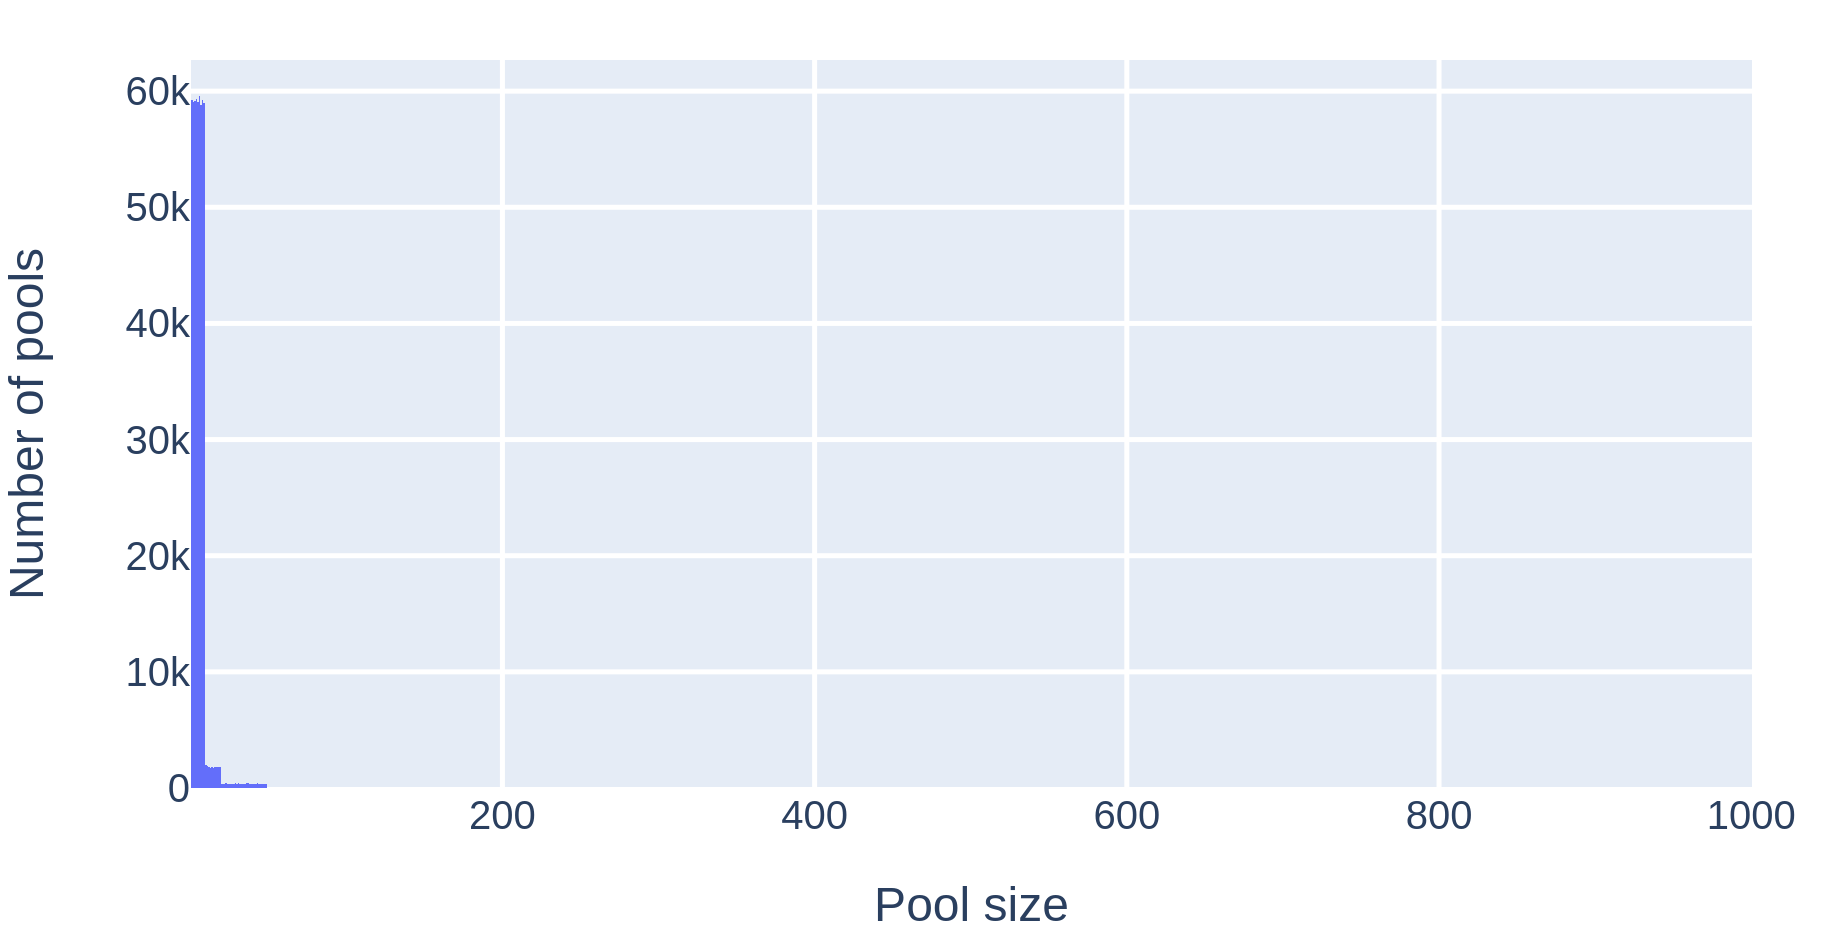
\includegraphics[width=.8\textwidth]{3 - Stride/fig/workplace_all_poolsizes.png}
    \caption{Distribution of the workplace pool sizes in the 11M population.}
    \label{fig:workplace_all_poolsizes}
\end{figure}

\begin{figure} 
  \begin{subfigure}[b]{0.5\linewidth}
    \centering
    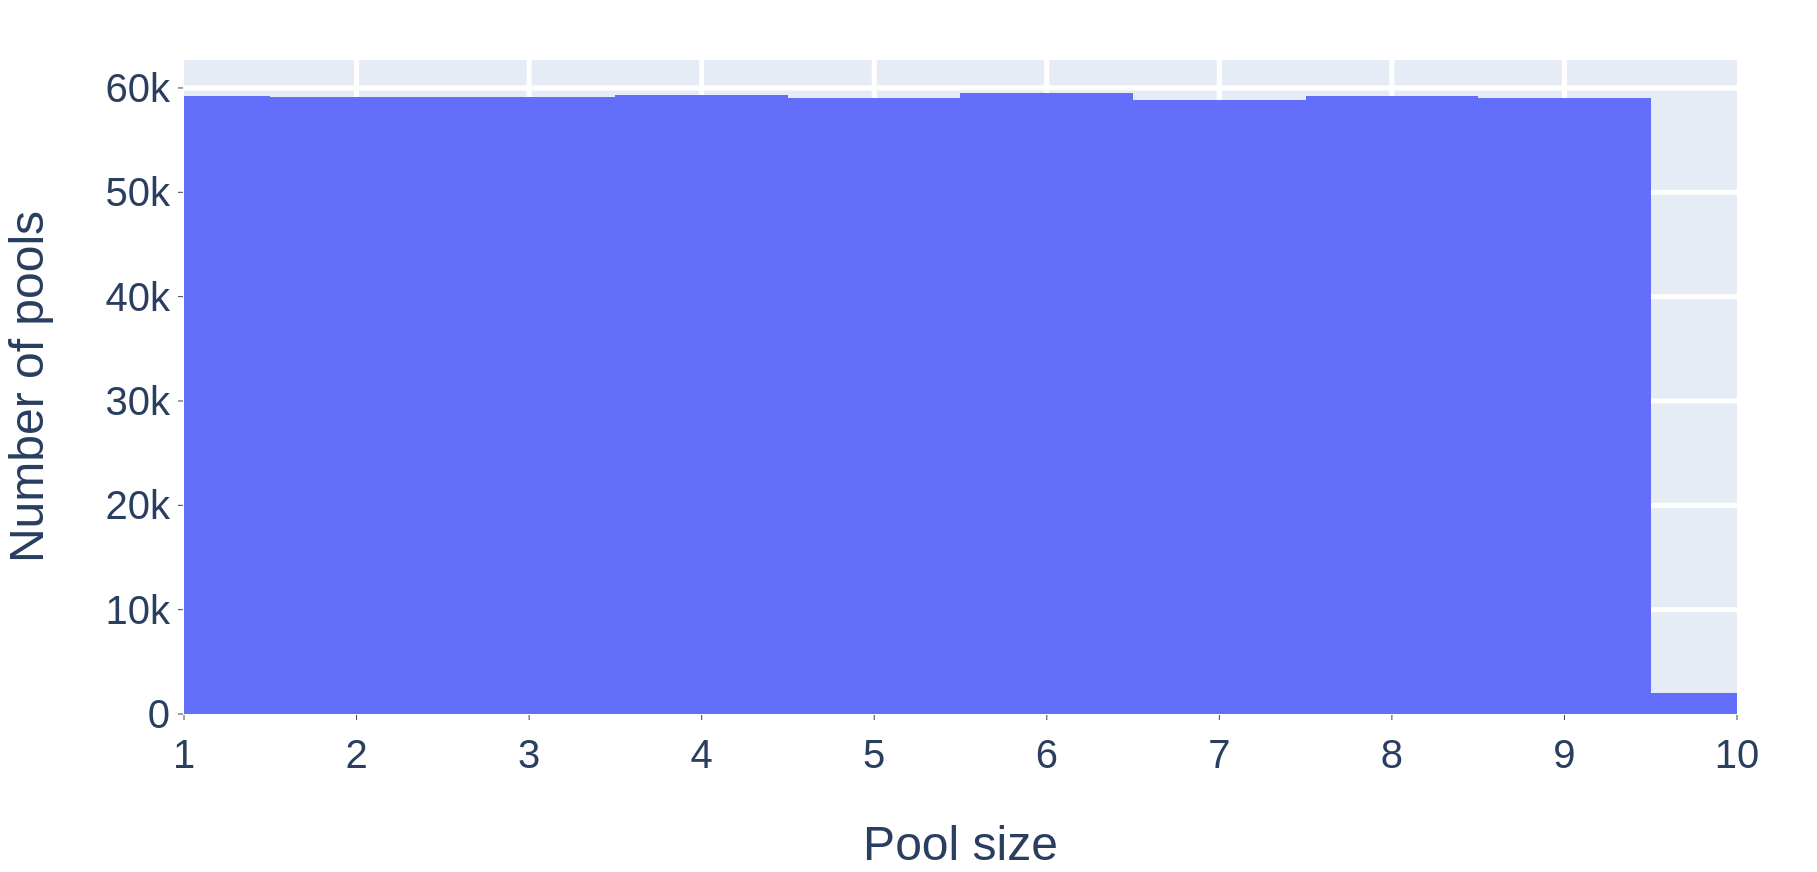
\includegraphics[width=\linewidth]{3 - Stride/fig/workplace_1-10_poolsizes.png} 
    \caption{Pool sizes 1 to 10.} 
    \label{fig:workplace_1-10_poolsizes} 
    \vspace{4ex}
  \end{subfigure}%% 
  \begin{subfigure}[b]{0.5\linewidth}
    \centering
    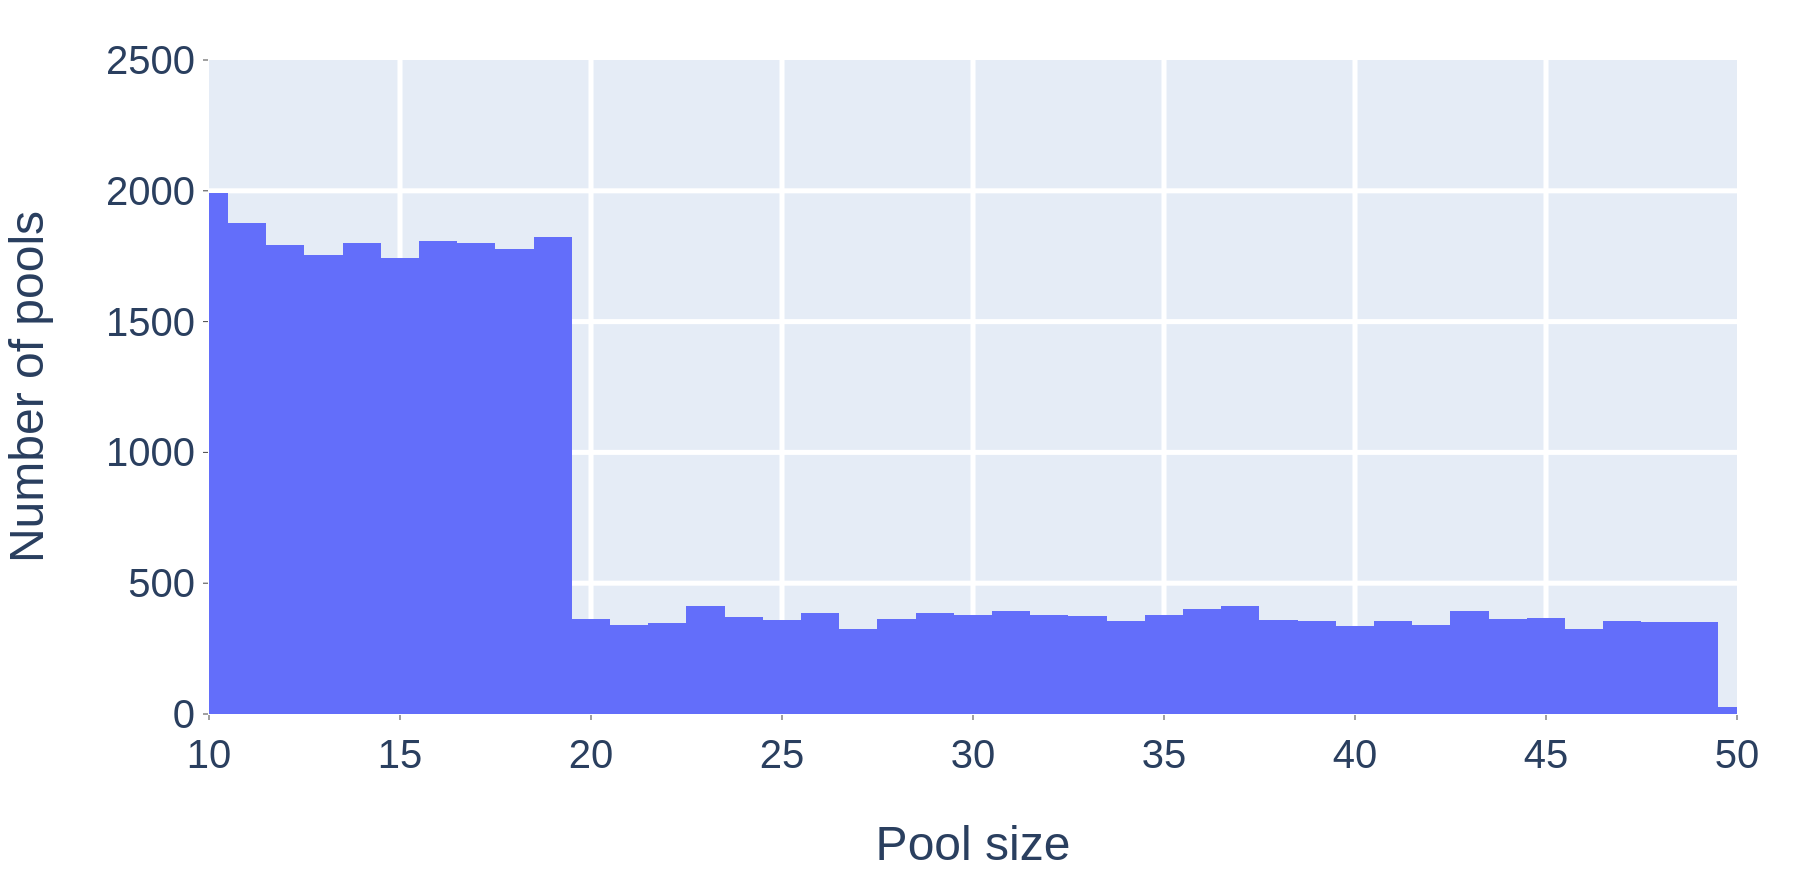
\includegraphics[width=\linewidth]{3 - Stride/fig/workplace_10-50_poolsizes.png} 
    \caption{Pool sizes 10 to 50.} 
    \label{fig:workplace_10-50_poolsizes} 
    \vspace{4ex}
  \end{subfigure} 
  \begin{subfigure}[b]{0.5\linewidth}
    \centering
    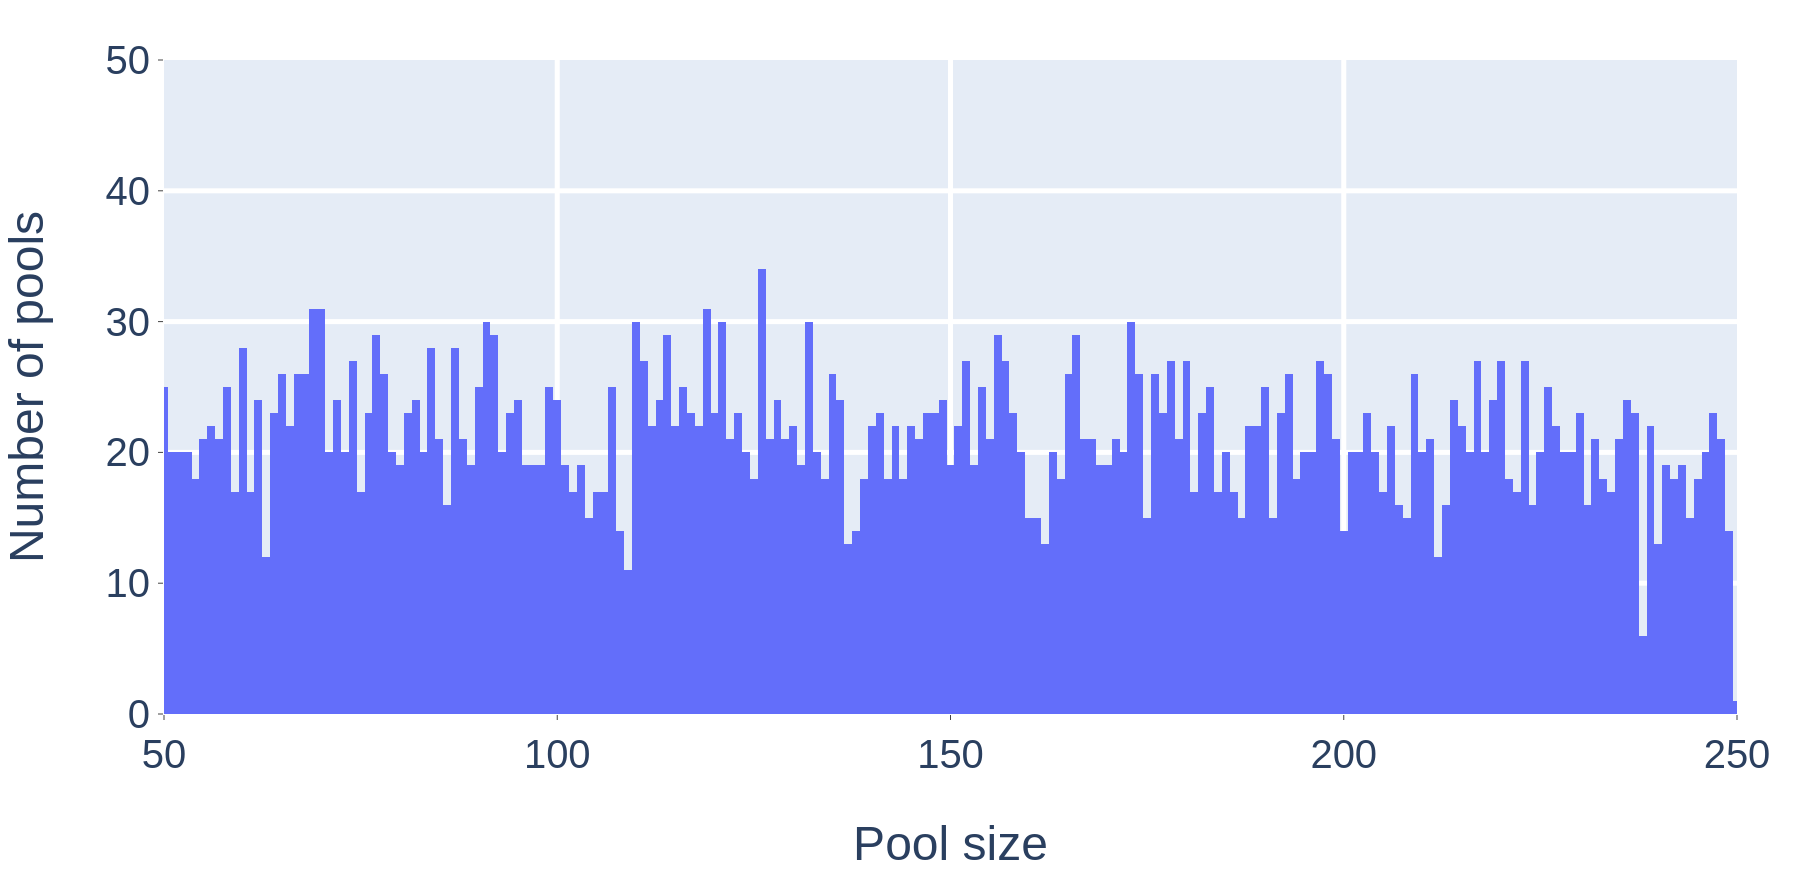
\includegraphics[width=\linewidth]{3 - Stride/fig/workplace_50-250_poolsizes.png} 
    \caption{Pool sizes 50 to 250.} 
    \label{fig:workplace_5-250_poolsizes} 
  \end{subfigure}%%
  \begin{subfigure}[b]{0.5\linewidth}
    \centering
    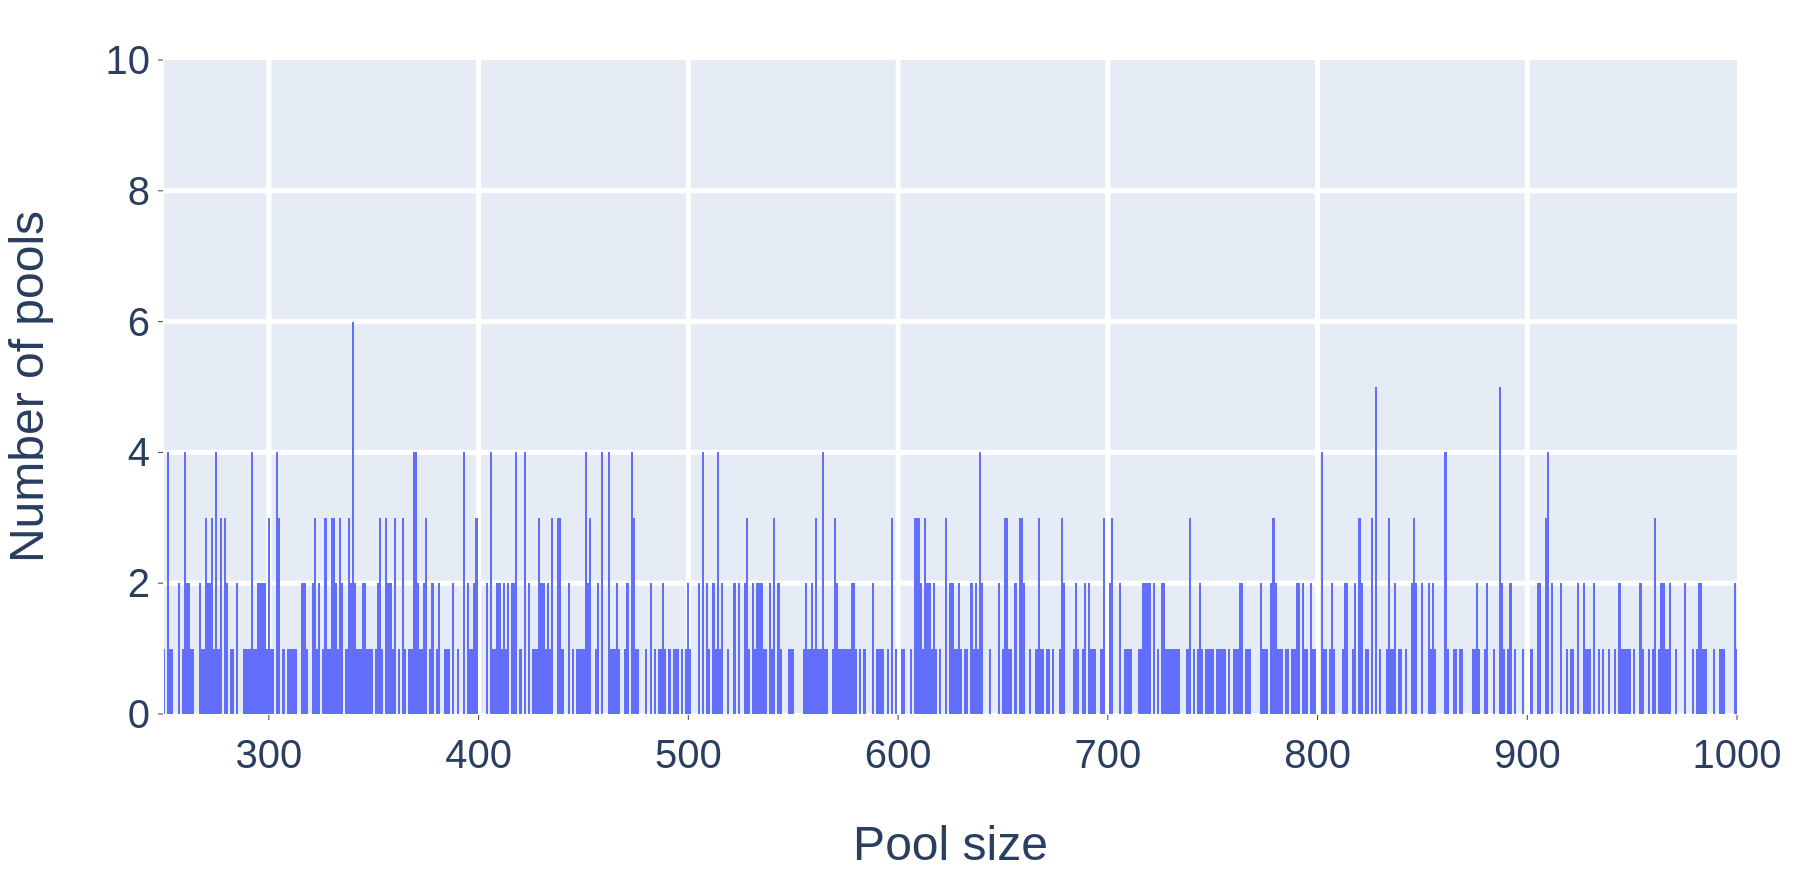
\includegraphics[width=\linewidth]{3 - Stride/fig/workplace_250-1000_poolsizes.png} 
    \caption{Pool sizes 250 to 1000.} 
    \label{fig:workplace_250-1000_poolsizes} 
  \end{subfigure} 
  \caption{Distributions of the workplace pool sizes from Figure \ref{fig:workplace_all_poolsizes} for different pool size ranges.}
  \label{fig:workplace_poolsize_ranges} 
\end{figure}

\begin{table}
\centering
\resizebox{\textwidth}{!}{%
\begin{tabular}{@{}lrrrrr@{}}
\toprule
Pool size range      & 1 - 9     & 10 - 19 & 20 - 49 & 50 - 249 & 250 - 1000 \\ \midrule
\begin{tabular}[t]{@{}l@{}}Minimum number of pools\\ (for a pool size)\end{tabular} &
  58,827 &
  1,744 &
  324 &
  \begin{tabular}[t]{@{}r@{}}6\\(11 excl. size 238)\end{tabular} &
  1 \\
\begin{tabular}[t]{@{}l@{}}Maximum number of pools\\ (for a pool size)\end{tabular} &
  59,547 &
  1,992 &
  414 &
  34 &
  6 \\ \midrule
Number of pools      & 532,518   & 18,169  & 10,983  & 4,286    & 803        \\
\% of pools          & 94.0      & 3.2     & 1.9     & 0.8      & 0.1        \\ \midrule
Number of people     & 2,661,724 & 262,427 & 377,612 & 629,345  & 467,110    \\
\% of working people & 60.5      & 6.0     & 8.6     & 14.3     & 10.6       \\ \bottomrule
\end{tabular}%
}
\caption{Statistics for the different workplace pool size ranges. The pool sizes in every size range have approximately the same amount of pools.}
\label{tab:workplace_stats}
\end{table}

\subsubsection{Primary \& secondary community}
When we looked at the general statistics of the community pool types, we noticed that the primary and secondary community contact pools had very similar results. Figures \ref{fig:primary_community_poolsizes} and \ref{fig:secondary_cumminity_poolsizes} demonstrate that these types of pools are nearly identical and both have a normal pool size distribution with a peak around size 500.

\begin{figure}
    \centering
    \begin{minipage}[b]{0.48\textwidth}
        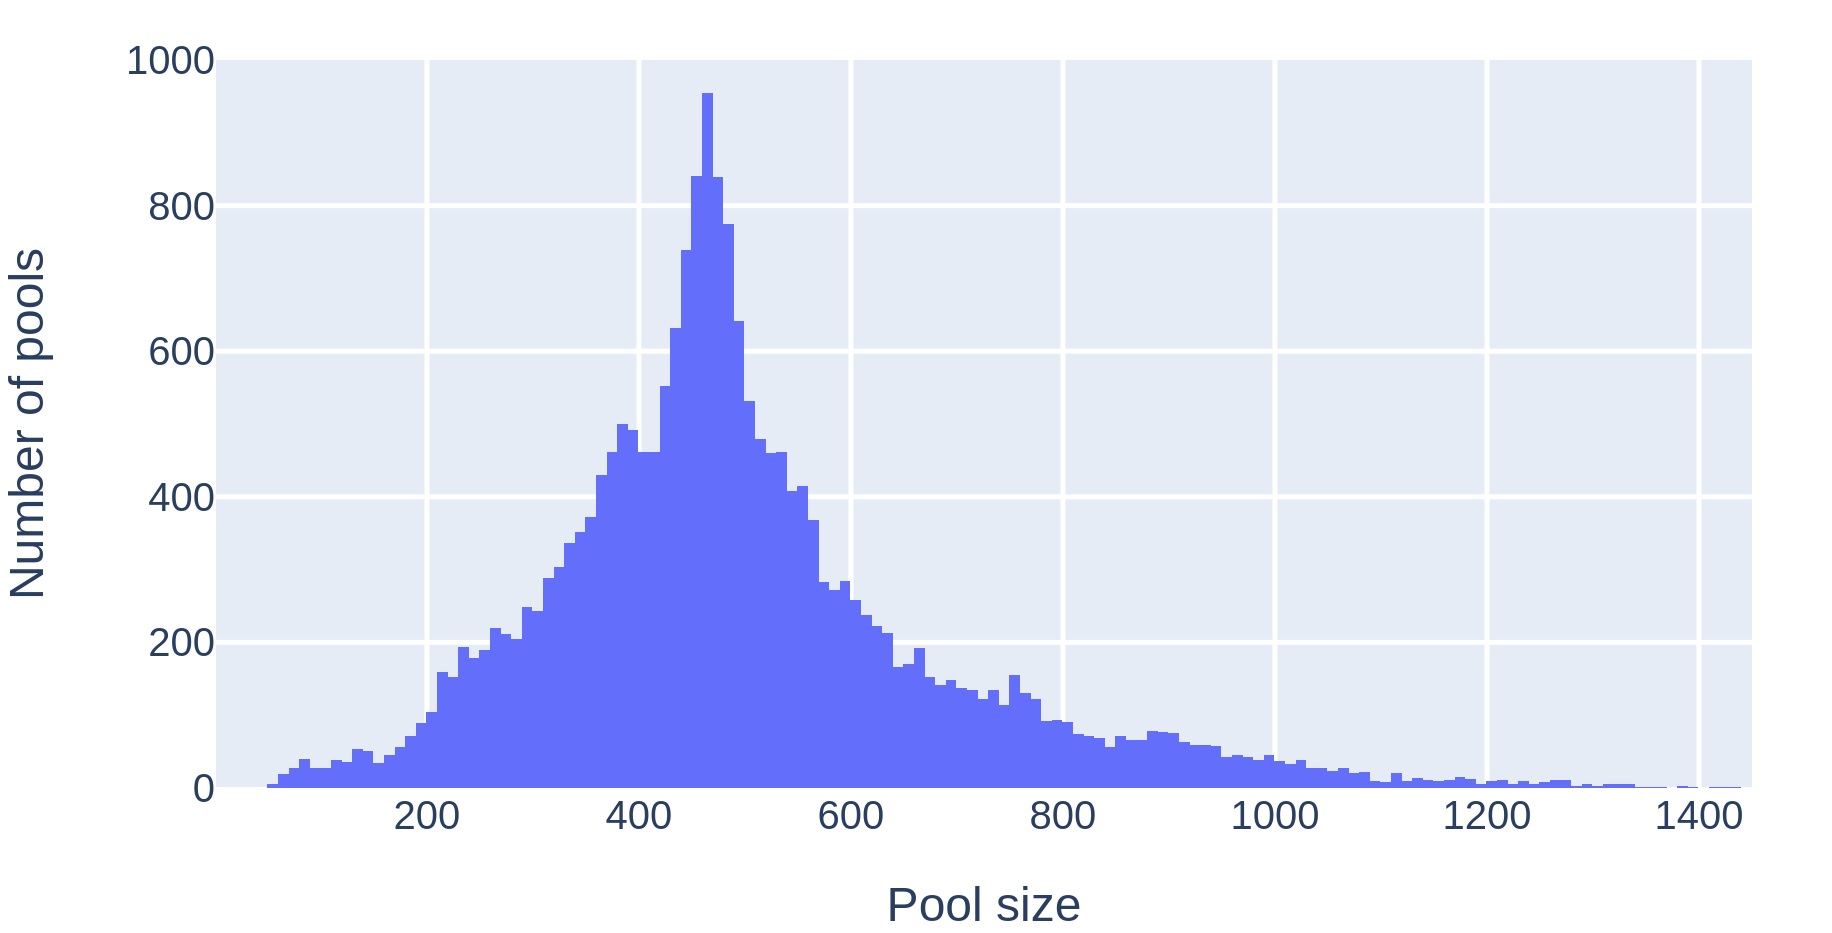
\includegraphics[width=\textwidth]{3 - Stride/fig/primary_community_poolsizes.png}
        \caption{Distribution of the primary community pool sizes of the 11M population.}
        \label{fig:primary_community_poolsizes}
    \end{minipage}
    \hfill
    \begin{minipage}[b]{0.48\textwidth}
        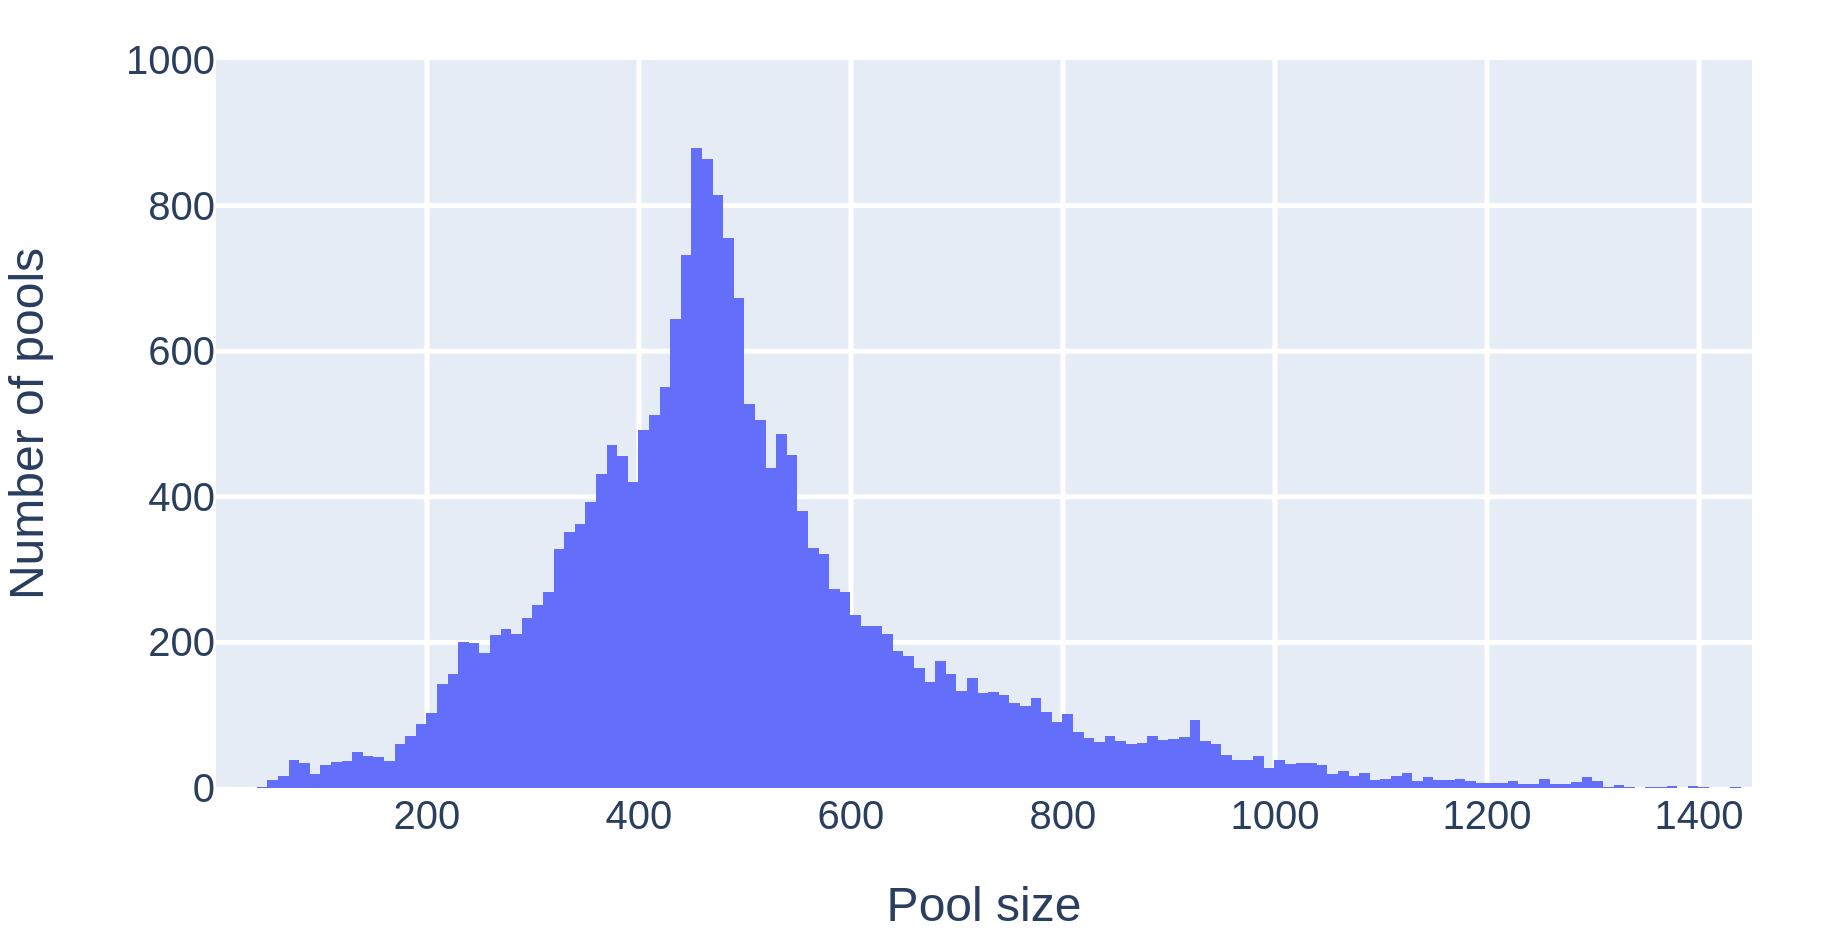
\includegraphics[width=\textwidth]{3 - Stride/fig/secondary_community_poolsizes.png}
        \caption{Distribution of the secondary community pool sizes of the 11M population.}
        \label{fig:secondary_cumminity_poolsizes}
    \end{minipage}
\end{figure}

\subsection{Contact matrix}
\label{subsec:contact_matrix}
In Section \ref{subsec:contacts_and_transmissions} we learned how Stride calculates a contact probability based on the configurated contact matrices, which was explained in Section \ref{subsec:configurations}. For every type of contact pool there exists a matrix which contains the contact rate based on age. The matrices for a school, workplace, primary community, and secondary community are respectively displayed in Figures \ref{fig:school_contact_rates}, \ref{fig:work_contact_rates}, \ref{fig:primary_contact_rates}, and \ref{fig:secondary_contact_rates}. These rates indicate the average number of contacts an individual has in a particular contact pool with respect to their own age. Algorithm \ref{alg:contact_probability} shows how the contact probability gets calculated between two individuals. The probability of two people having contact in a household is always $0.999$, therefore, we do not need a contact matrix for the household contact pool type.
\\\\
The data for these contact rates originates from SOCRATES, which is an online interactive tool\footnote{\url{http://www.socialcontactdata.org/socrates/}}, created by Willem et al. \cite{socrates}, for the sharing of social contact data. The data they present are 2D matrices in which the contact rate in a pool is based on the ages of the person who initiates contact and the one who receives it. These matrices for our contact pool types are visualised in Figure \ref{fig:contact_heatmaps}, which are different than the ones we presented. The contact rates that Stride uses are actually 1D matrices or just \textit{vectors}, which are based on those 2D matrices. These matrices have been transformed into our vectors so that contact rate look-ups are faster and easier to use. If we would use the actual matrices, with dimensions 112x112, the look-ups would take substantially more time than with our vectors. Thus, from now on we will refer to these 1D matrices as the \textit{contact vectors}. Furthermore, in the 2D matrices we again clearly see that people have the most contact with people who are the same age, with an exception in the workplace. This exception has an intuitive explanation, which is that people at work have contact with everyone disregarding age and that people at work are mostly between the ages of 18 to 65 years old. 

\begin{figure}
    \centering
    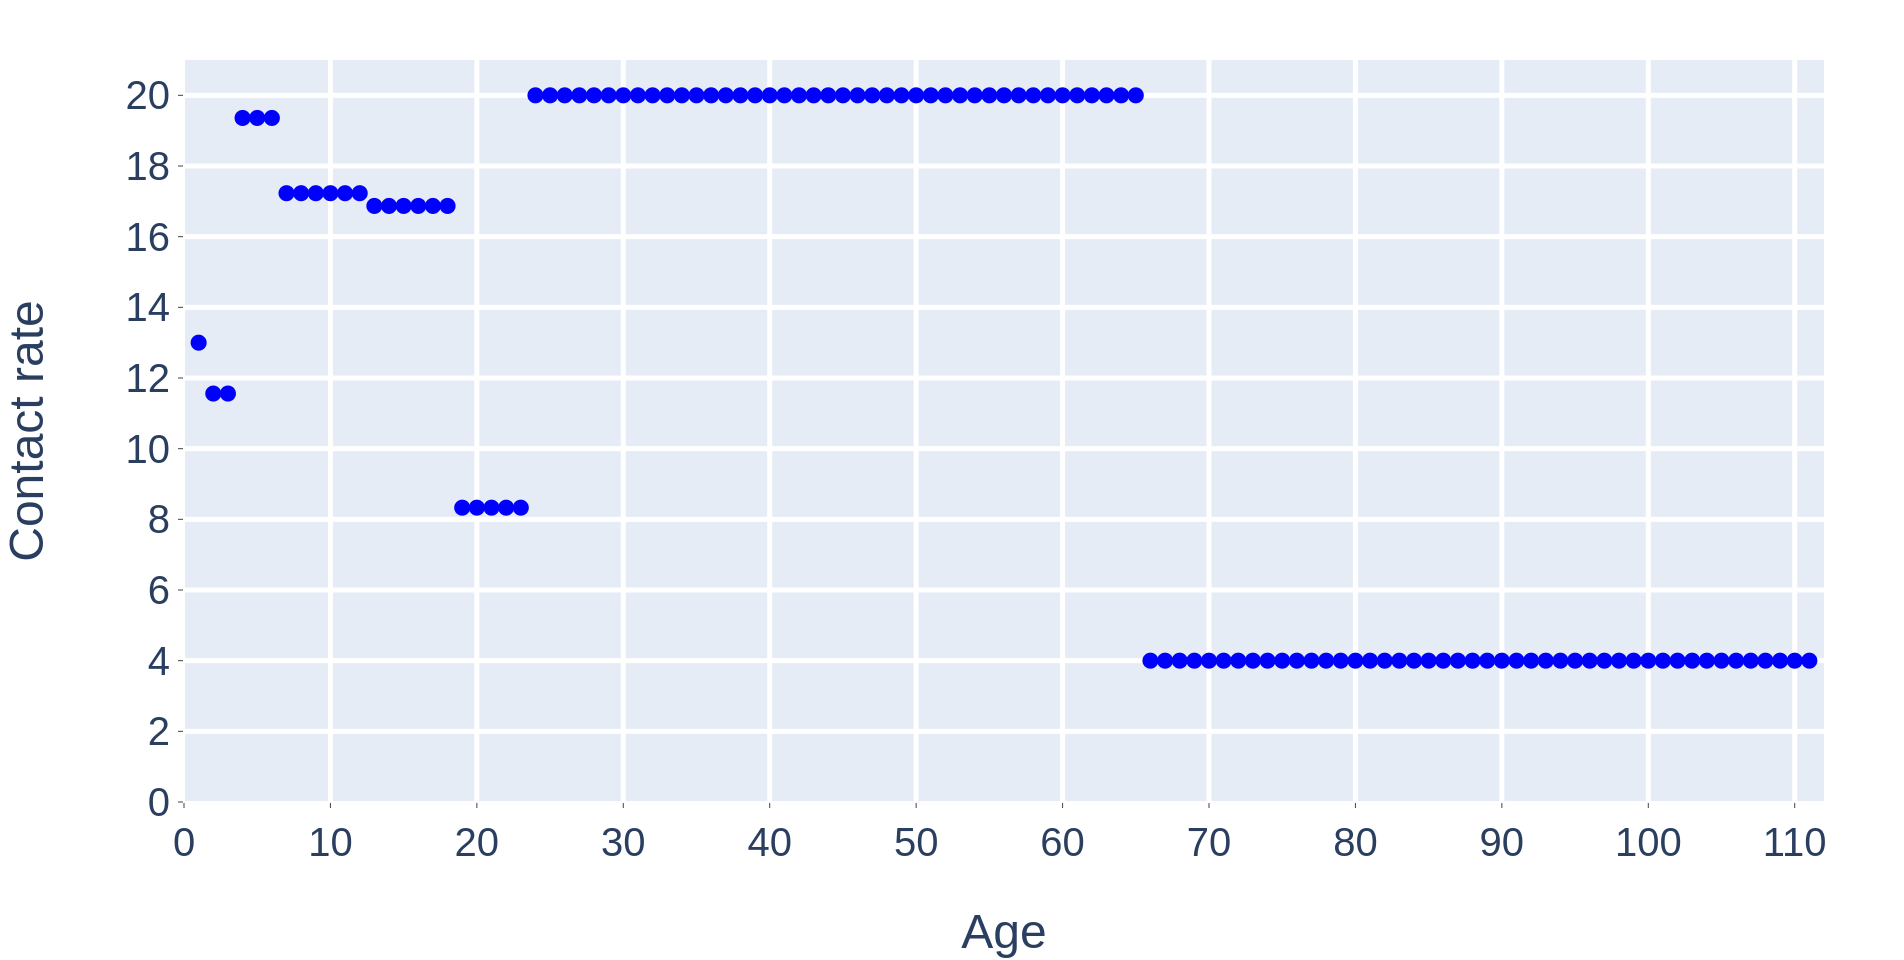
\includegraphics[width=.8\textwidth]{3 - Stride/fig/school_contact_rates.png}
    \caption{Contact rates per age at school.}
    \label{fig:school_contact_rates}
\end{figure}

\begin{figure}
    \centering
    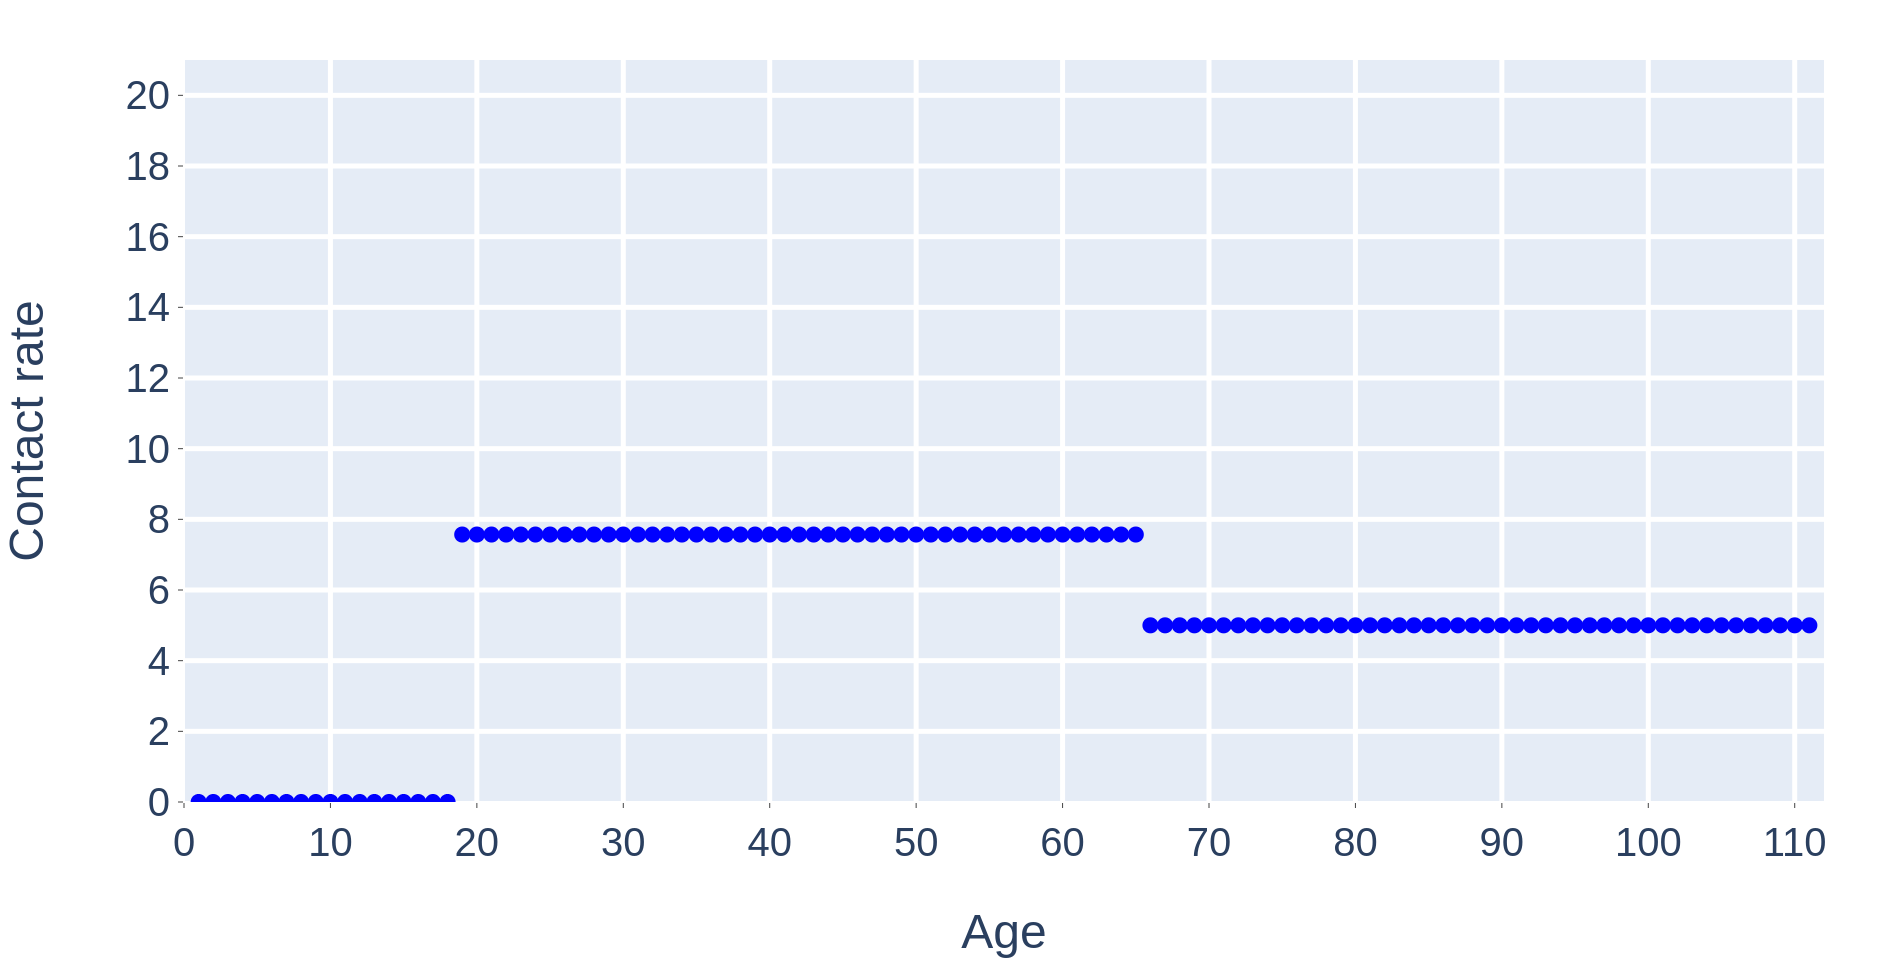
\includegraphics[width=.8\textwidth]{3 - Stride/fig/work_contact_rates.png}
    \caption{Contact rates per age at work.}
    \label{fig:work_contact_rates}
\end{figure}

\begin{figure}
    \centering
    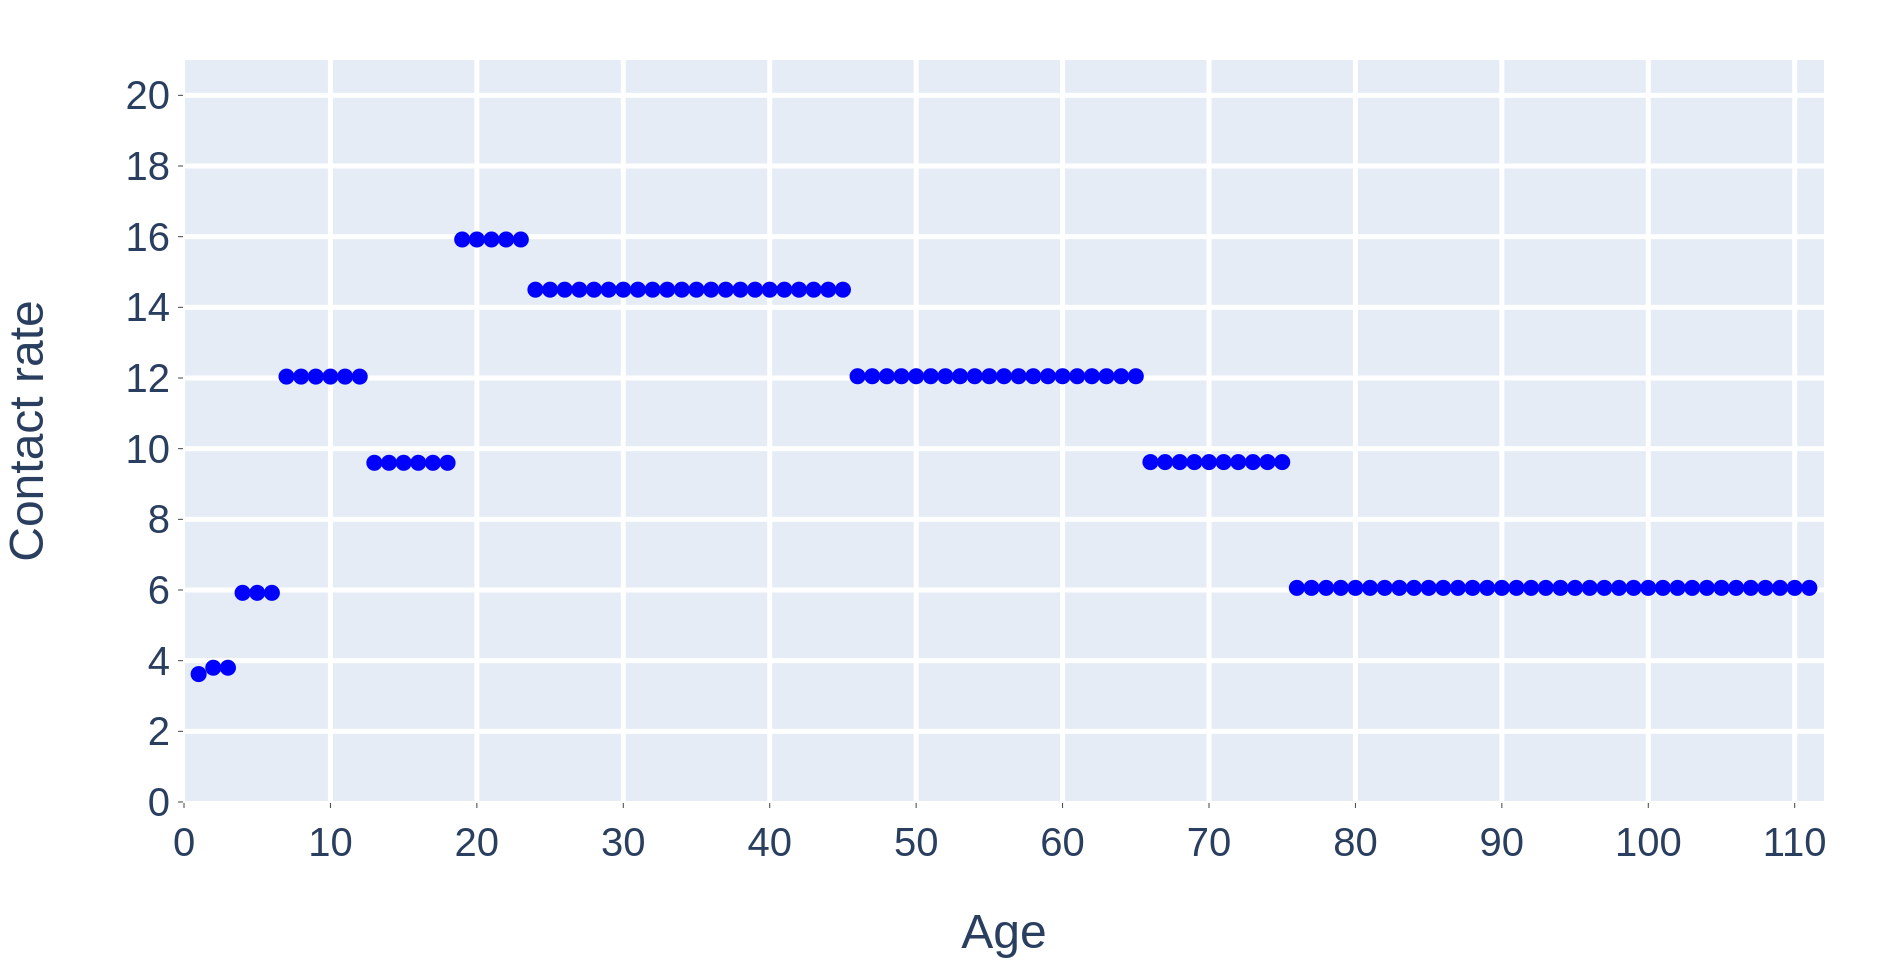
\includegraphics[width=.8\textwidth]{3 - Stride/fig/primary_contact_rates.png}
    \caption{Contact rates per age in a primary community.}
    \label{fig:primary_contact_rates}
\end{figure}

\begin{figure}
    \centering
    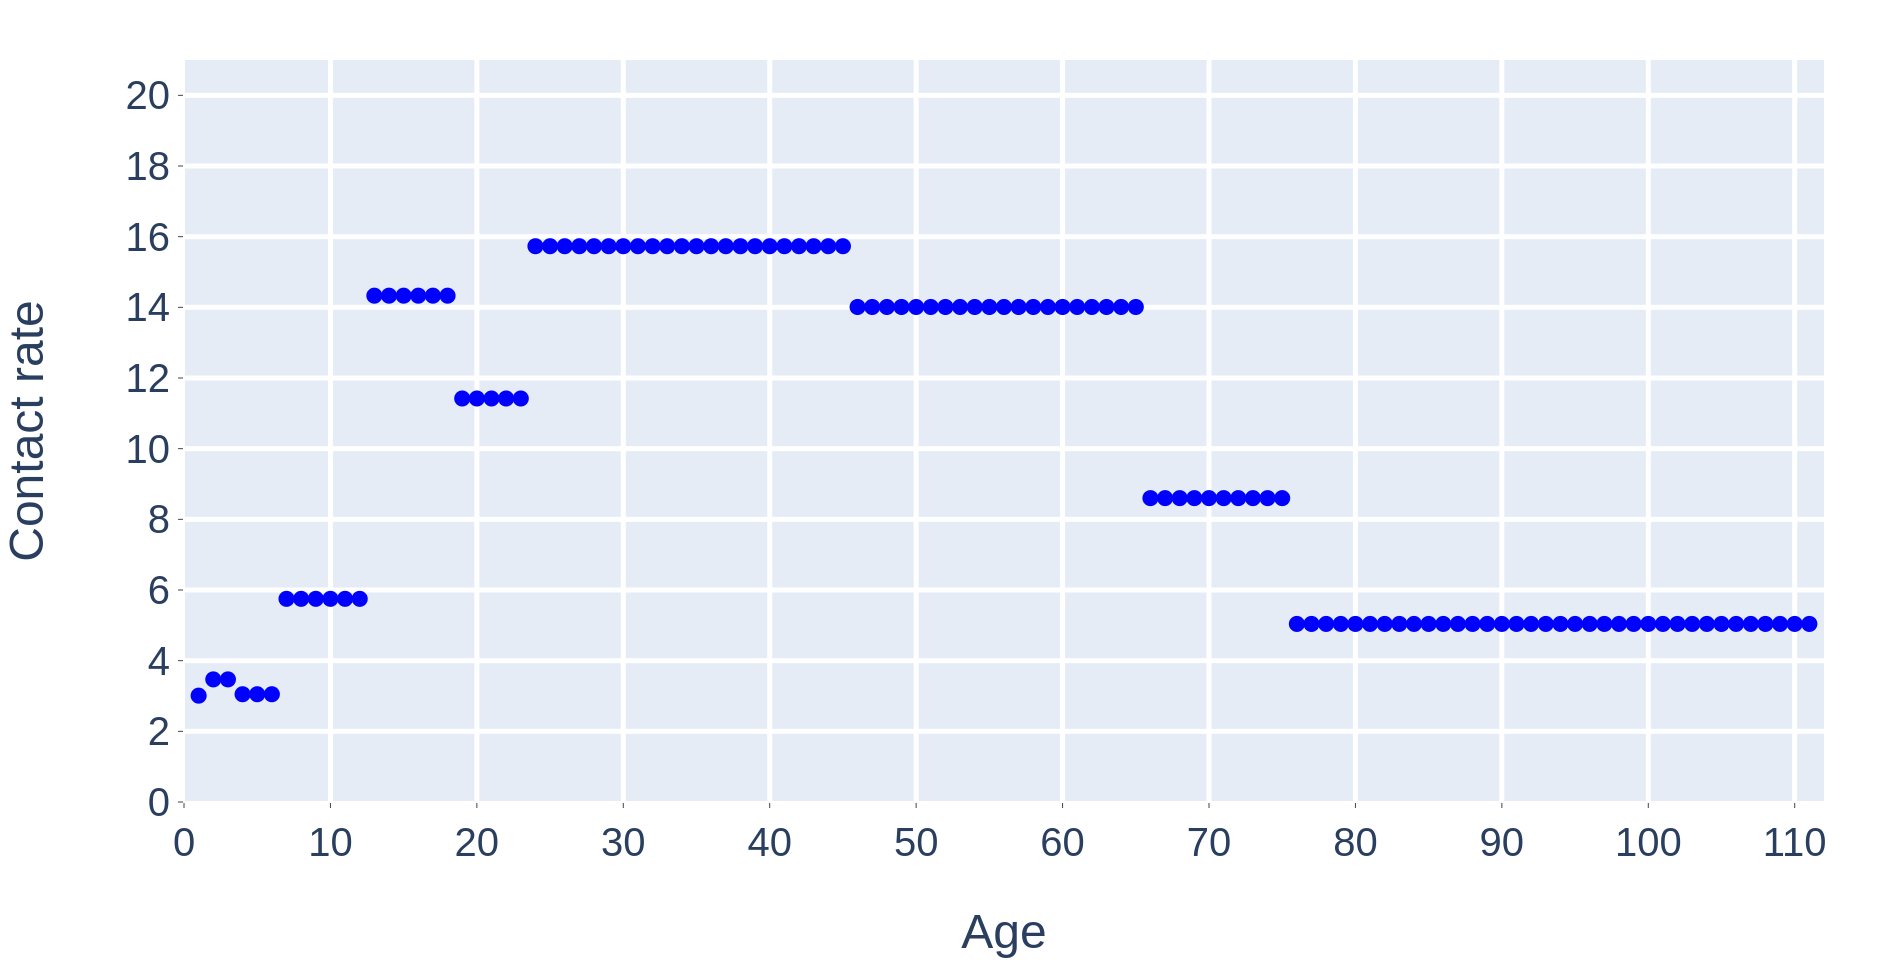
\includegraphics[width=.8\textwidth]{3 - Stride/fig/secondary_contact_rates.png}
    \caption{Contact rates per age in a secondary community.}
    \label{fig:secondary_contact_rates}
\end{figure}

%-------------------------

\begin{figure} 
  \begin{subfigure}[b]{0.45\linewidth}
    \centering
    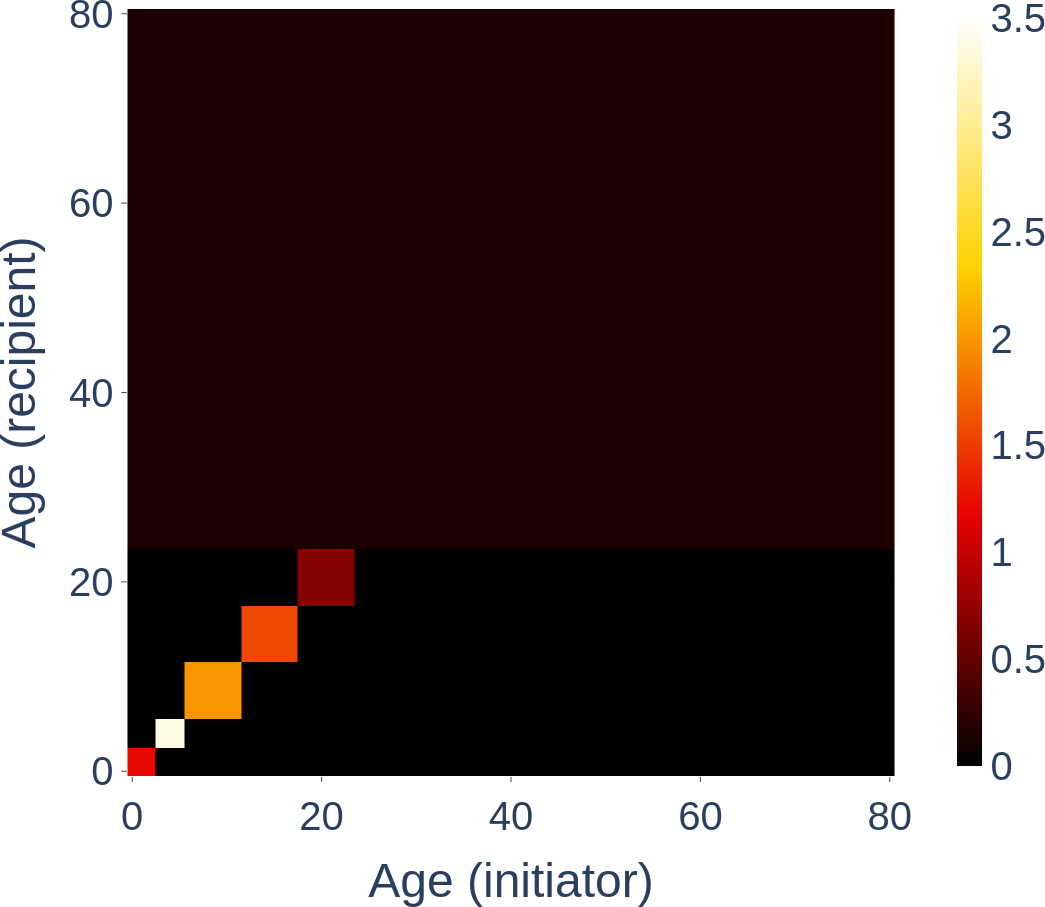
\includegraphics[width=\linewidth]{3 - Stride/fig/school_contact_heatmap.png} 
    \caption{School.} 
    \label{fig:school_contact_heatmap} 
    \vspace{4ex}
  \end{subfigure}%% 
  \hfill
  \begin{subfigure}[b]{0.45\linewidth}
    \centering
    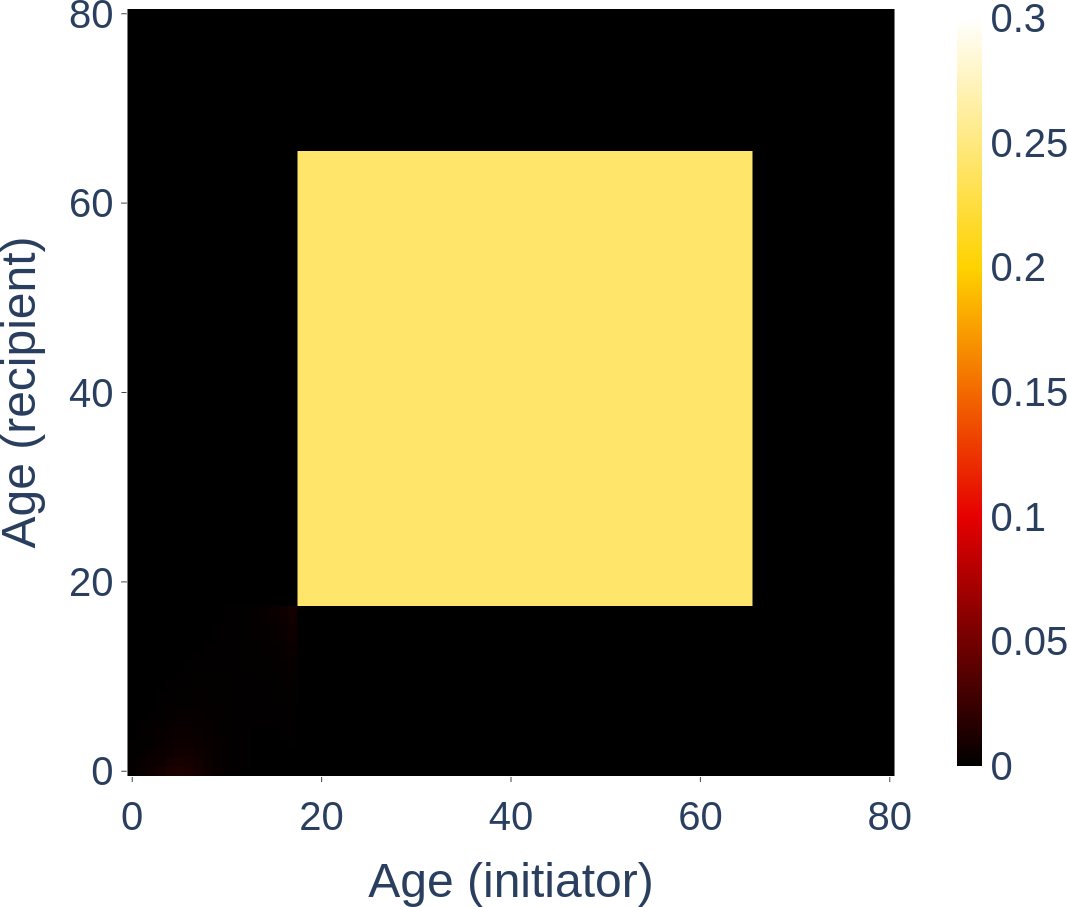
\includegraphics[width=\linewidth]{3 - Stride/fig/work_contact_heatmap.png} 
    \caption{Workplace.} 
    \label{fig:workplace_contact_heatmap} 
    \vspace{4ex}
  \end{subfigure}
  \begin{subfigure}[b]{0.45\linewidth}
    \centering
    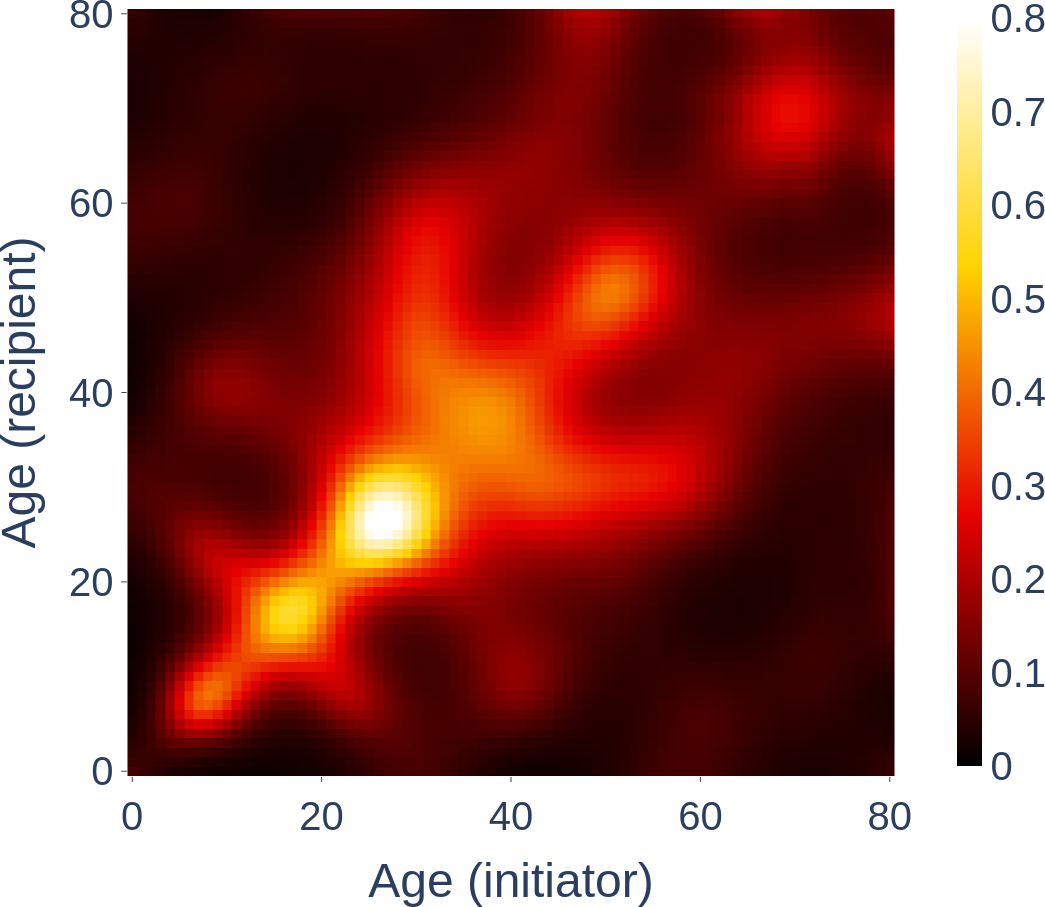
\includegraphics[width=\linewidth]{3 - Stride/fig/primary_contact_heatmap.png} 
    \caption{Primary community.} 
    \label{fig:primary_contact_heatmap} 
  \end{subfigure}%%
  \hfill
  \begin{subfigure}[b]{0.45\linewidth}
    \centering
    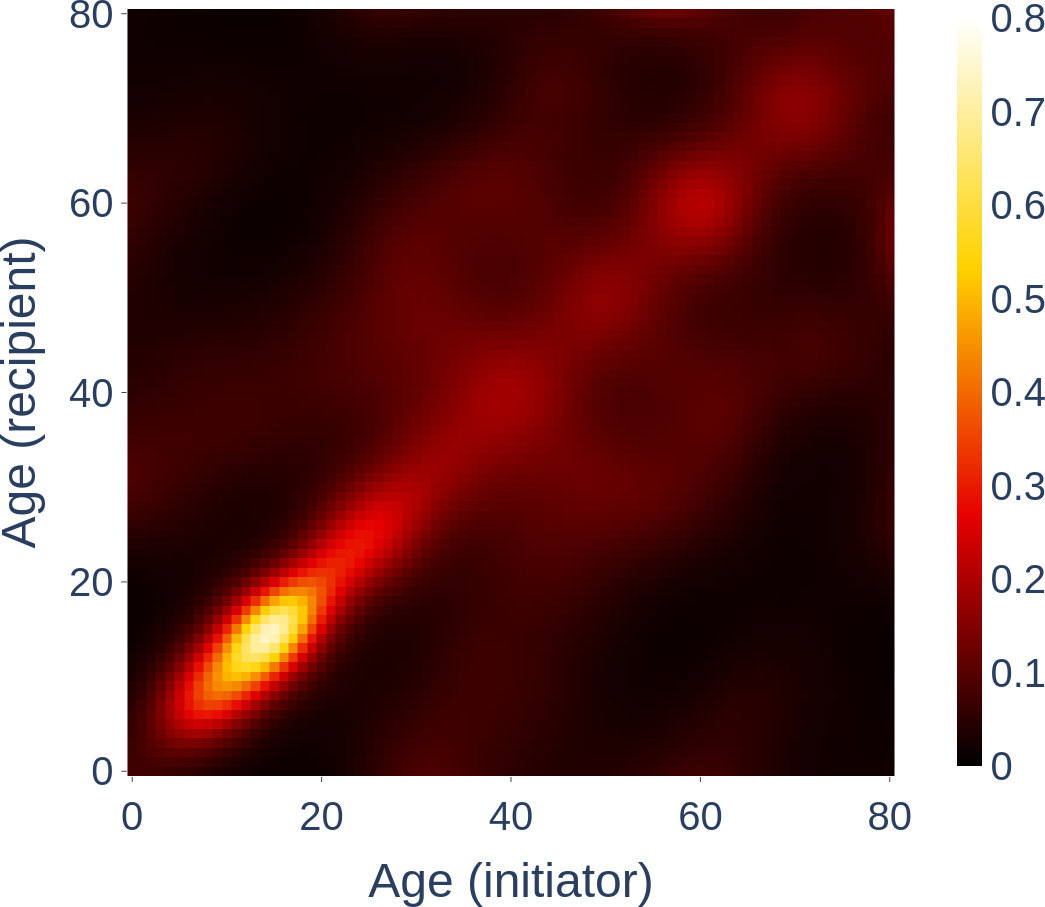
\includegraphics[width=\linewidth]{3 - Stride/fig/secondary_contact_heatmap.png} 
    \caption{Secondary community.} 
    \label{fig:secondary_contact_heatmap} 
  \end{subfigure} 
  \caption{2D contact matrix heatmaps showing the contact rates based on the ages of the contact initiator and recipient.}
  \label{fig:contact_heatmaps} 
\end{figure}

\section{Analysis}
\label{sec:analysis}
Now that we have a complete understanding of Stride, we can dig into the code and start to analyse it. 

\subsection{Parallellization}
A well-known optimisation technique in programming is called \textit{parallellization}, which is the act of executing multiple parts of the program simultaneously. This can only be applied when a program allows for its code to be run in parallel. There are various parallellization techniques and each has its own pros and cons, so which one is most suitable depends on the situation. Stride also uses such a technique and it is called OpenMP\footnote{\url{https://www.openmp.org/}}.
\\\\
In computer science, a thread (of execution) is a term used to describe the smallest sequence of program instructions that can be run independently \cite{multiprocess_programs}. OpenMP is an implementation of multithreading, which is the act of executing multiple threads concurrently and it is managed by the CPU (central processing unit). A thread runs on a core of a CPU and such a core can execute multiple threads concurrently. A core can only execute one thread at a time, so when there are multiple threads that need to be executed by a core, some need to wait their turn. If we were to use multithreading on a single core, the program would become slower instead of faster, because the threads would still be run sequentially and there would be overhead from the CPU who has to manage the threads. CPUs nowadays have multiple cores which allows us to divide the threads on the cores. When we now want to use OpenMP, we need to check the number of cores our CPU has. We then use this number to tell our program the maximum number of threads it can use for the most optimal run time.
\\\\
An important aspect of OpenMP is that CPU cores share their memory. How this memory sharing exactly works depends on the CPU, but these details do not belong to the scope of this thesis. However, this can become an issue when working with a lot of data which, as we will see, is the case for Stride.

\subsection{Code}
In Section \ref{sec:simulation} we explained how a Stride simulation works, which was also visualised in Figure \ref{fig:simulation_flow}. Every part of the simulation process will we now examine separately while we simultaneously think about possible ways to improve the code that we are looking at.

\subsubsection{Initialisation}
We have seen that the initialisation consists of reading the configurations and setting up the simulation accordingly. Most of these configurations are values that have an effect on how the simulation has to run and what information it has to produce, but they only take one hundredth of a second and can thus be ignored. The first major portion is reading the 11M population file, which translates to reading 11 million rows and creating an individual for every single row. This is done in sequence by reading row after row and creating a person every time and storing it in the population. Reading this file could be done in parallel, but trying to store the individuals concurrently in the population would probably cause more harm than good due to the threads that need to store something in the same memory.
\\\\
After the population and contact pools have been created, it is turn to the seeders to determine the individuals' health characteristics, the people who are immune, and the people who start infected. These seeders are already optimised by using OpenMP where possible.

\subsubsection{Updating individuals}
The next step in our code is the update of every individual. This consists of updating a person's health status, as seen in Section \ref{subsec:health_status_update}, and then immediately updating the pools in which the person will be present for the upcoming day, as seen in Section \ref{subsec:pool_presences}. Stride iterates over the entire population and updates every individual separately, but this iteration is implemented with the possibility to use OpenMP. This, together with the fact that the updates are very small functions, indicates that there will probably be not much room to improve Stride here.

\subsubsection{Contact tracing}
As we know from Section \ref{subsec:contact_tracing}, it is possible to use a contact tracing feature in Stride. This code section iterates twice over the population without OpenMP, so this could already be a potential optimisation by parallellizing the iterations. However, because this part of the code does not belong to the standard simulation, we give this section the lowest priority when making improvements. Besides these iterations the contact tracing performs some operations that need to be done and cannot be changed or improved.

\subsubsection{Calculating contacts and transmissions}
Section \ref{subsec:contacts_and_transmissions} explained the core of Stride, which is how contacts and transmissions get calculated. There are two algorithms for this: \textsc{All-to-All} and \textsc{Inf-to-Sus}. Only one of these can be used when simulating a day and this is determined at runtime. They are both implemented in a template called \textit{infector} and how Stride executes this for every pool is shown in Algorithm \ref{alg:infector}, which consists of pseudo code combined with the actual OpenMP calls for completeness. We iterate over all the contact pool types and check if the type of pool is active in the current day and if not, we skip this type of pool. If we are, for example, simulating a holiday, we skip the workplace type. If the type of pool is active, we then iterate over every pool of that type and send them to the infector. During this thesis, several questions and concerns arose about this implementation, which we will now discuss:
\begin{enumerate}
    \item \textbf{We calculate the contacts and transmissions for every pool of every type in one large iteration, how does this affect the results?}
    
    The order in which we do all these calculations does not matter that much. When someone becomes exposed, it always takes at least a day before they get infected or start feeling symptoms. Therefore, they will not be able to infect someone in the same iteration or change their behaviour.
    
    \item \textbf{When we use OpenMP, is there a possibility that problems occur regarding memory read and write operations? For example when two pools are being processed by infector and they consist of overlapping individuals.}
    
    The parallellization only applies to the inner for-loop which iterates over all the pools of a particular type. We have seen that people can only be a member of one pool per pool type, so this rule prevents such issues.
    
    \item \textbf{At line 9 in Algorithm \ref{alg:infector} the population is passed on to infector. Why would this be necessary and does this present problems regarding OpenMP?}
    
    The population is needed in infector because it gets used when calculating the contact probabilities, although we did not explicitly show this in Algorithm \ref{alg:contact_probability}. This does not cause any issues because the population is wrapped in a shared pointer, as we will see in Section \ref{subsec:first_opt_updating_individuals}.
    
    \item \textbf{We learned that the contacts and transmissions depend on randomness. Since randomness has to be created via random number generators, would this not cause problems when using OpenMP?}
    
    In Section \ref{subsec:initialisation} we discussed how random number generator (RNG) managers are the first thing that get created in the initialisation step. Stride creates such RNG managers for every thread and passes these on to infector, as we see in line 9 of Algorithm \ref{alg:infector}, which takes care of any issues regarding random number generators with multithreading.
\end{enumerate}

\begin{algorithm}
\caption{Pseudo code of how \textit{infector} is used on every pool in a simulation day.}
\label{alg:infector}
\begin{algorithmic}[1]
    \State \textbf{\#pragma} omp parallel num\_threads(m\_num\_threads)
    \State \{
    \State $thread\_num \gets$ \Call{omp\_get\_thread\_num}{\null}
    \Foreach{$type$ in  $pooltypes[\;]$} \Comment{Iterate over pool types}
        \If{$type$ not active}
            \State continue \Comment{Ignore this type and go to the next}
        \EndIf
        \State \textbf{\#pragma} omp for schedule(static)
        \Foreach{$pool$ in $pools[type]$} \Comment{Iterate over every pool of $type$}
            \State \Call{infector}{$pool, population, rng\_handler[thread\_num], ...$}
        \EndForeach
    \EndForeach
    \State \}
\end{algorithmic}
\end{algorithm}

\subsection{Performance}
\label{subsec:performance}
A first code examination of Stride taught us more about the different components of the program and how parallellization is already used to improve the simulation speed. Our next step is to run the simulation with different parameters and measure the performance. All simulations in this chapter and the next use the configurations described in Appendix \ref{appendix:configurations} unless stated otherwise. \paragraph{VSC} All of the following tests in this chapter and Chapter \ref{chapter:sampling} ran on the VSC\footnote{\url{https://www.vscentrum.be/}} (Vlaams Supercomputer Centrum, or in English Flemish Supercomputer Centre) to get the most optimal results with the least amount of external interference. Our tests ran on (cascadelake) computer nodes with a Xeon Gold 6240 CPU@2.6 GHz with 18 cores; 192 GB RAM; 200 GB SSD local disk. \textsc{All-to-All} simulations have memory and virtual memory peaks of respectively 9.5 GB and 10.2 GB, while \textsc{Inf-to-Sus} only has peaks of 3.1 GB memory and 3.3 GB virtual memory. Memory bandwidth and latency measurements can be found on the VSC website\footnote{\url{https://docs.vscentrum.be/en/latest/leuven/tier2_hardware/memory_bandwidth_and_latency_tier2.html\#memory-bandwidth-and-latency-cascadelake-tier2}}.
\\\\
For our performance tests we divide the model in three sections and measure the time of each section as well as the total time. The sections are: updating individuals, contact tracing, and calculating contacts and transmissions (which we will now refer to as infector). With our first test, we want to see how much time Stride spends per section each day for both infector algorithms. The results for these simulations using \textsc{All-to-All} and \textsc{Inf-to-Sus} are visualised in Figure \ref{fig:basis_runtime_sections}. The average results per section are listed in Table \ref{tab:basis_runtime_stats}. The small runtime differences, such as the updating and tracing sections for both algorithms, are due to low-level system details and are negligible for the rest of this thesis.
\\\\
We notice from our results that the \textsc{Inf-to-Sus} is a major runtime optimisation compared to \textsc{All-to-All}, which is all due to the difference in the infector algorithm. When Stride uses \textsc{All-to-All}, almost all of its time is spend in the infector, so this is where we should look for improvements first. The ups and downs that we see in both graphs are caused by the type of day, 5 weekdays and 2 weekend days, where the weekdays take a little bit more time. This is a logical effect because the weekdays have more active pools (household, work, K-12 school, college, and secondary community) than weekend days (household, primary community).
\\\\
\textsc{Inf-to-Sus} displays a somewhat normal distribution regarding the infector time, with a peak around day 50. The explanation for this behaviour is that the infector only gets executed for a pool when at least one of its member is infectious. Figure \ref{fig:basis_infected} shows the number of people who are infected per simulation day. The number of people who are infected clearly matches these changes in runtime of the infector. The first day of this simulation also takes a lot more time than the following days, which is due to the sorting of the individuals based on their health status. At the start, these pools are initialised without sorting the members and thus it takes more time to sort them. When they get sorted the next day, there only need to be a few changes made on average which causes the sorting to be much faster.
\\\\
The total runtime of the entire 100-day simulation using \textsc{All-to-All} lasted 1 hour 43 minutes and 32 seconds, of which the initialisation took approximately 1 minute. The \textsc{Inf-to-Sus} simulation obviously needed the same amount of time for the initialisation, but ran in a total time of 5 minutes and 49 seconds. \textsc{Inf-to-Sus} only does calculations that are absolutely necessary and has therefore very little room for improvement compared to \textsc{All-to-All}. Our focus will thus not lie on the initialisation, because it is only a small percentage of the simulation when using \textsc{All-to-All}. Contact tracing needs the least amount by far, so we ignore this part from now on and will only mention it sometimes for the sake of completeness.

\begin{figure}
    \centering
      \begin{subfigure}[b]{\linewidth}
        \centering
        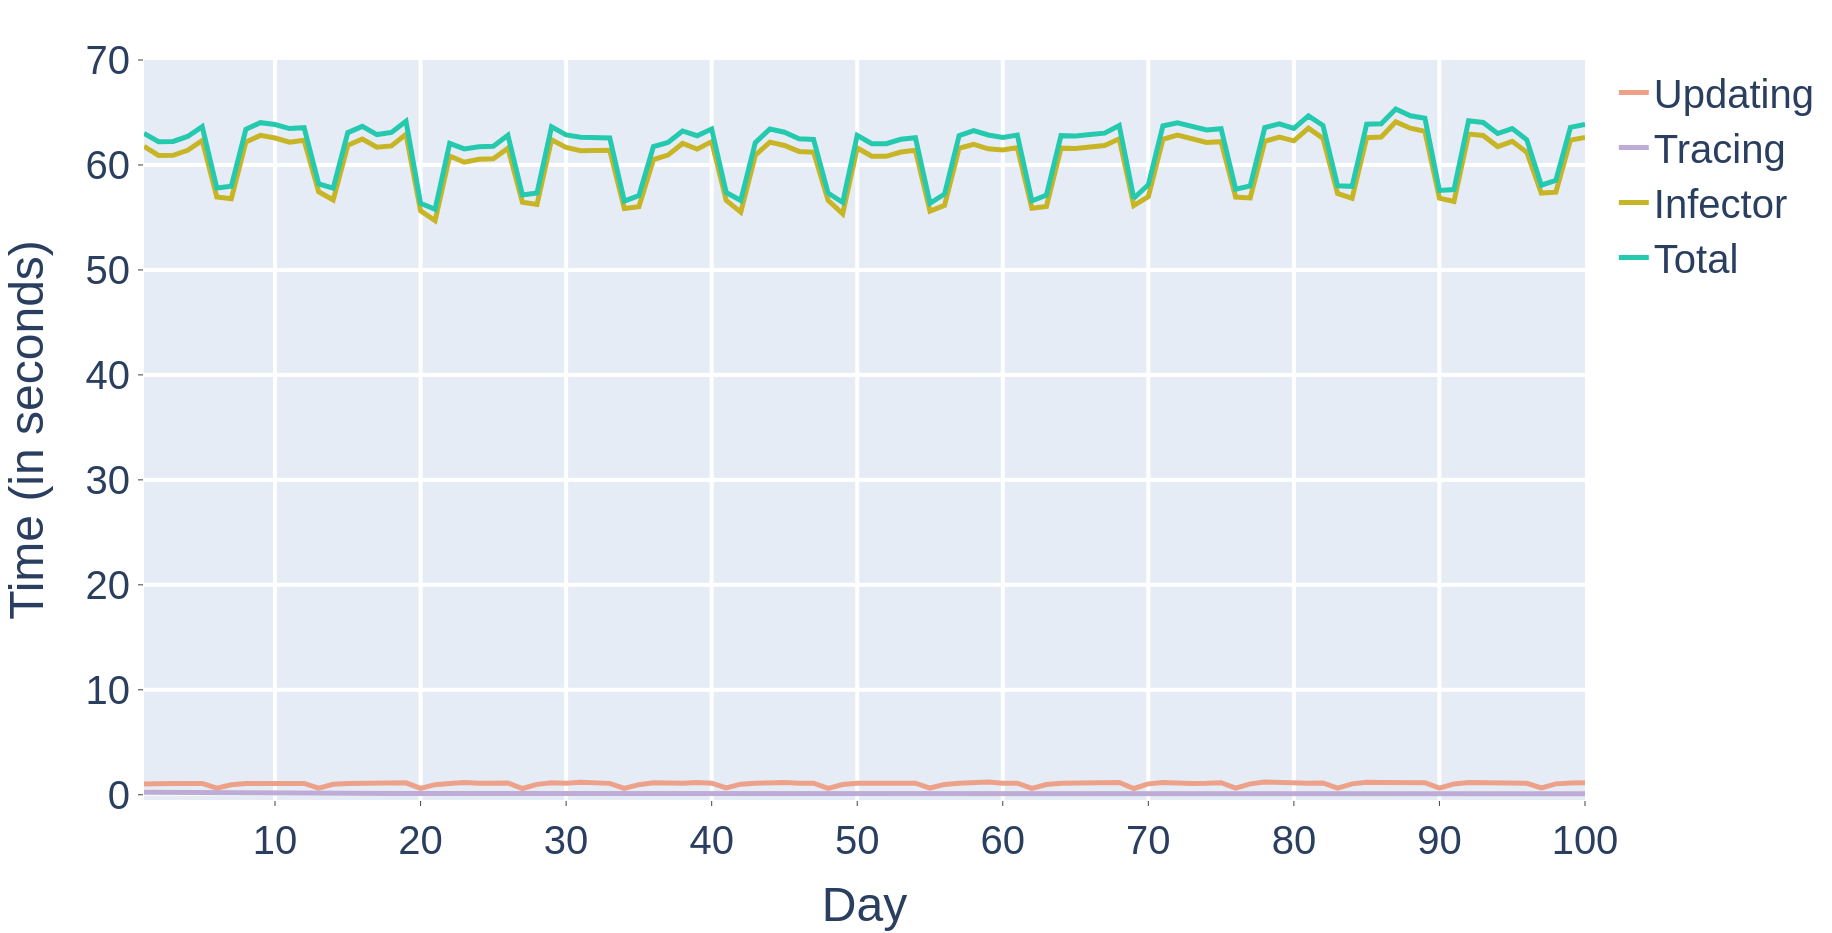
\includegraphics[width=\linewidth]{3 - Stride/fig/basis_all_runtime_sections.png} 
        \caption{\textsc{All-to-All}.} 
        \label{fig:basis_all_runtime_sections} 
      \end{subfigure}
      \begin{subfigure}[b]{\linewidth}
        \centering
        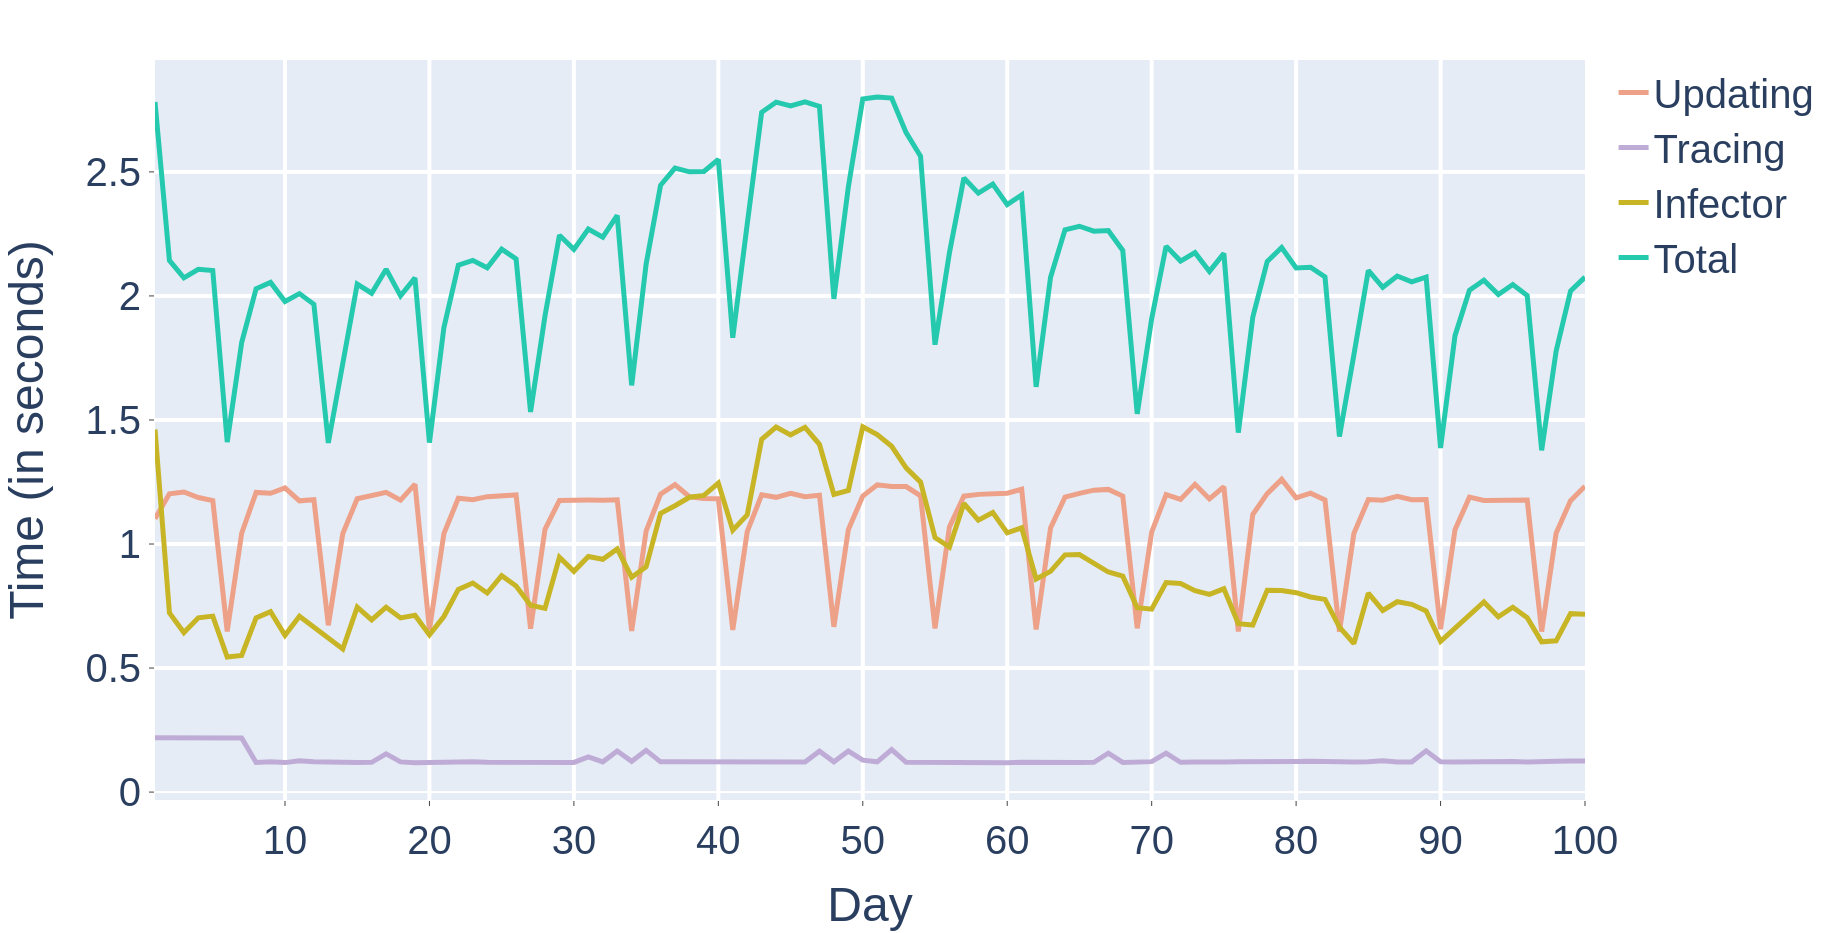
\includegraphics[width=\linewidth]{3 - Stride/fig/basis_opt_runtime_sections.png} 
        \caption{\textsc{Inf-to-Sus}.} 
        \label{fig:basis_opt_runtime_sections} 
      \end{subfigure} 
      \caption{Section times per day, in seconds, for every section, including the total times for simulating a day. Simulations run on 11M population for 100 days without holidays using 1 thread (configurations in Appendix \ref{appendix:configurations}).}
      \label{fig:basis_runtime_sections} 
\end{figure}

\begin{figure}
    \centering
    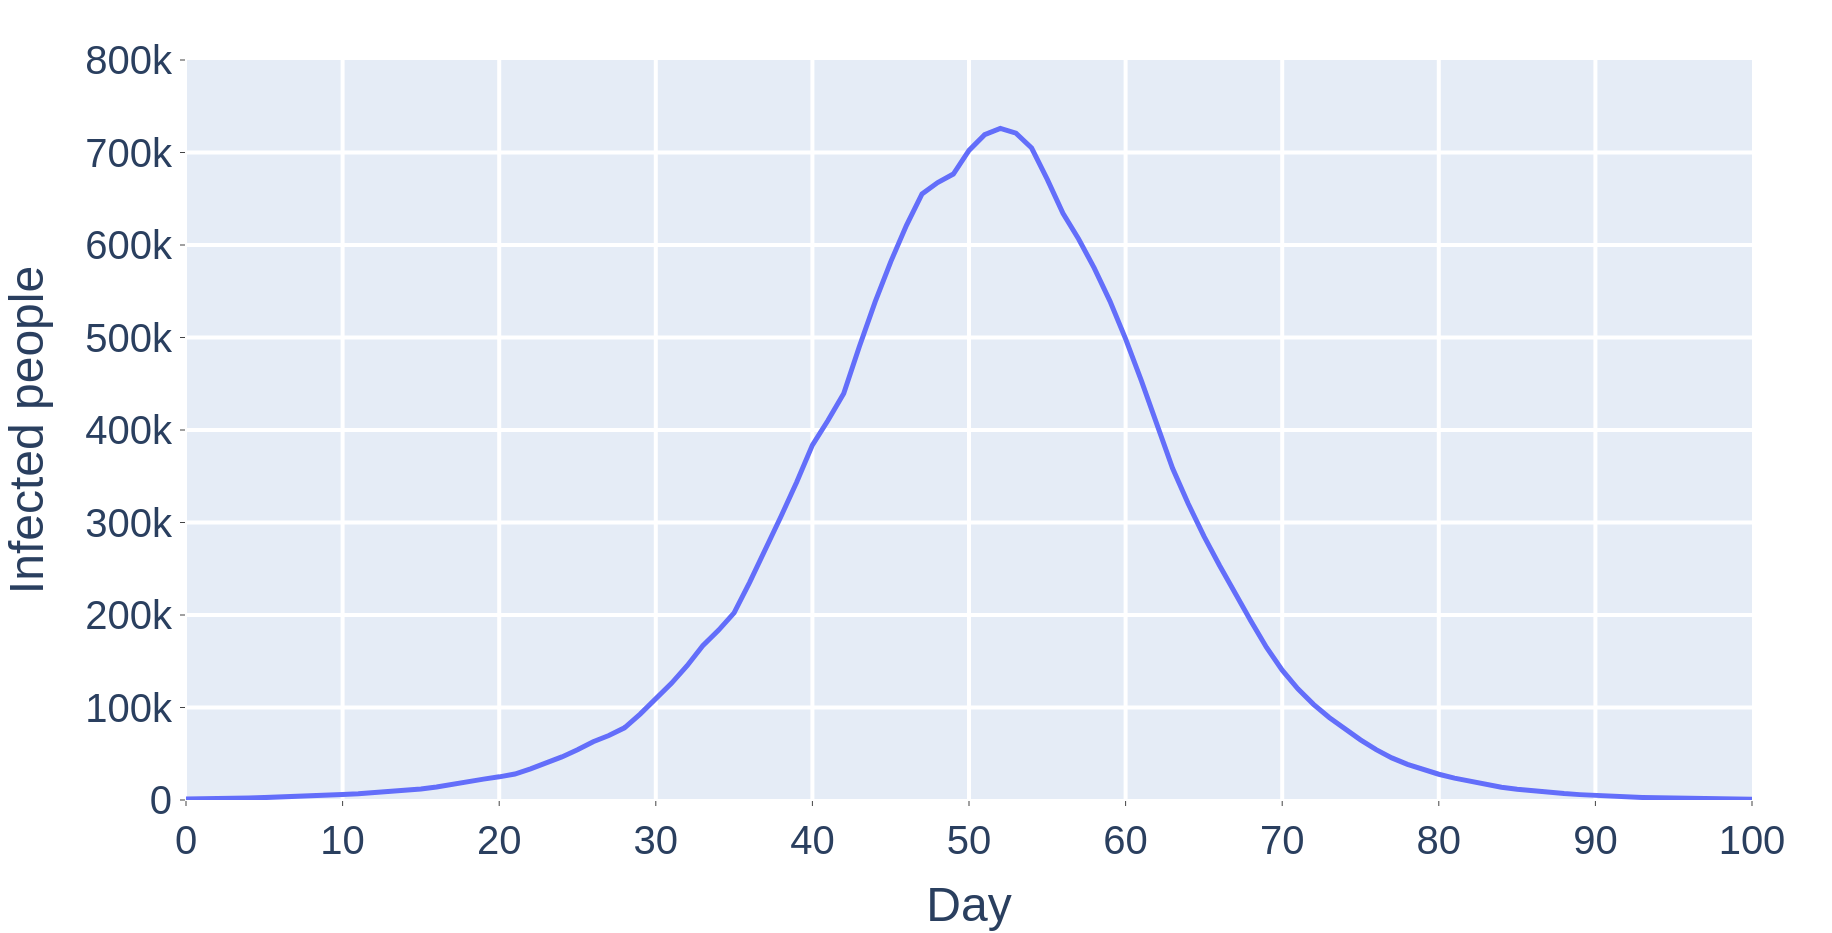
\includegraphics[width=.8\linewidth]{3 - Stride/fig/basis_infected.png}
    \caption{Number of infected people per simulation day. Simulation run on 11M population for 100 days without holidays using 1 thread (configurations in Appendix \ref{appendix:configurations}).}
    \label{fig:basis_infected}
\end{figure}

\begin{table}
\centering
\begin{tabular}{@{}lrrrr@{}}
\toprule
           & Updating & Tracing & Infector & Total \\ \midrule
All-to-All & 1.03     & 0.11    & 60.37    & 61.52 \\
Inf-to-Sus & 1.10     & 0.13    & 0.89     & 2.12  \\ \midrule
speedup    & /        & /       & 67.83    & 29.02 \\ \bottomrule
\end{tabular}
\caption{Average daily runtime (in seconds) per section. Simulations run on 11M population for 100 days without holidays using 1 thread (configurations in Appendix \ref{appendix:configurations}).}
\label{tab:basis_runtime_stats}
\end{table}

\subsubsection{Parallellization}
The next test that we will perform is to see how the previously implemented parallellization affects the runtimes, given that Stride is regularly expanded and updated, which could have harmed the parallellization performance. For this part, we will only focus on the parts of a simulation day that use OpenMP, which are the updating of individuals and the calculations of contacts and transmissions. Figure \ref{fig:basis_parallel_updating} reveals how the updating of individuals becomes slower when using more threads instead of faster. The implementation of OpenMP, which is supposed to be an improvement, has the opposite effect. We see a similar trend when looking at the \textsc{All-to-All} infector in Figure \ref{fig:basis_all_parallel_infector}. Here we notice that using two threads is the slowest and that using more threads than becomes gradually faster, although it is still much slower than the simulation without parallellization. The \textsc{Inf-to-Sus} infector exhibits rather strange behaviour regarding parallellization, which we can see in Figure \ref{fig:basis_opt_parallel_infector}. Using multiple threads is faster in the beginning and at the end of the simulation, but is slower in between. \textsc{Inf-to-Sus} has, just like \textsc{All-to-All}, the slowest times when using two threads and starts to become faster if more threads are used.
\\\\
In order to be more accurate, the average times per simulation day for all of these parallellization tests are displayed in Table \ref{tab:basis_parallel}. This confirms our statements about updating individuals and the \textsc{All-to-All} infector parallellization, but shows that multithreading is in fact faster on average for the \textsc{Inf-to-Sus} infector. However, the total simulation time is still higher when using multiple threads because of the updating of individuals.

\begin{figure}
    \centering
    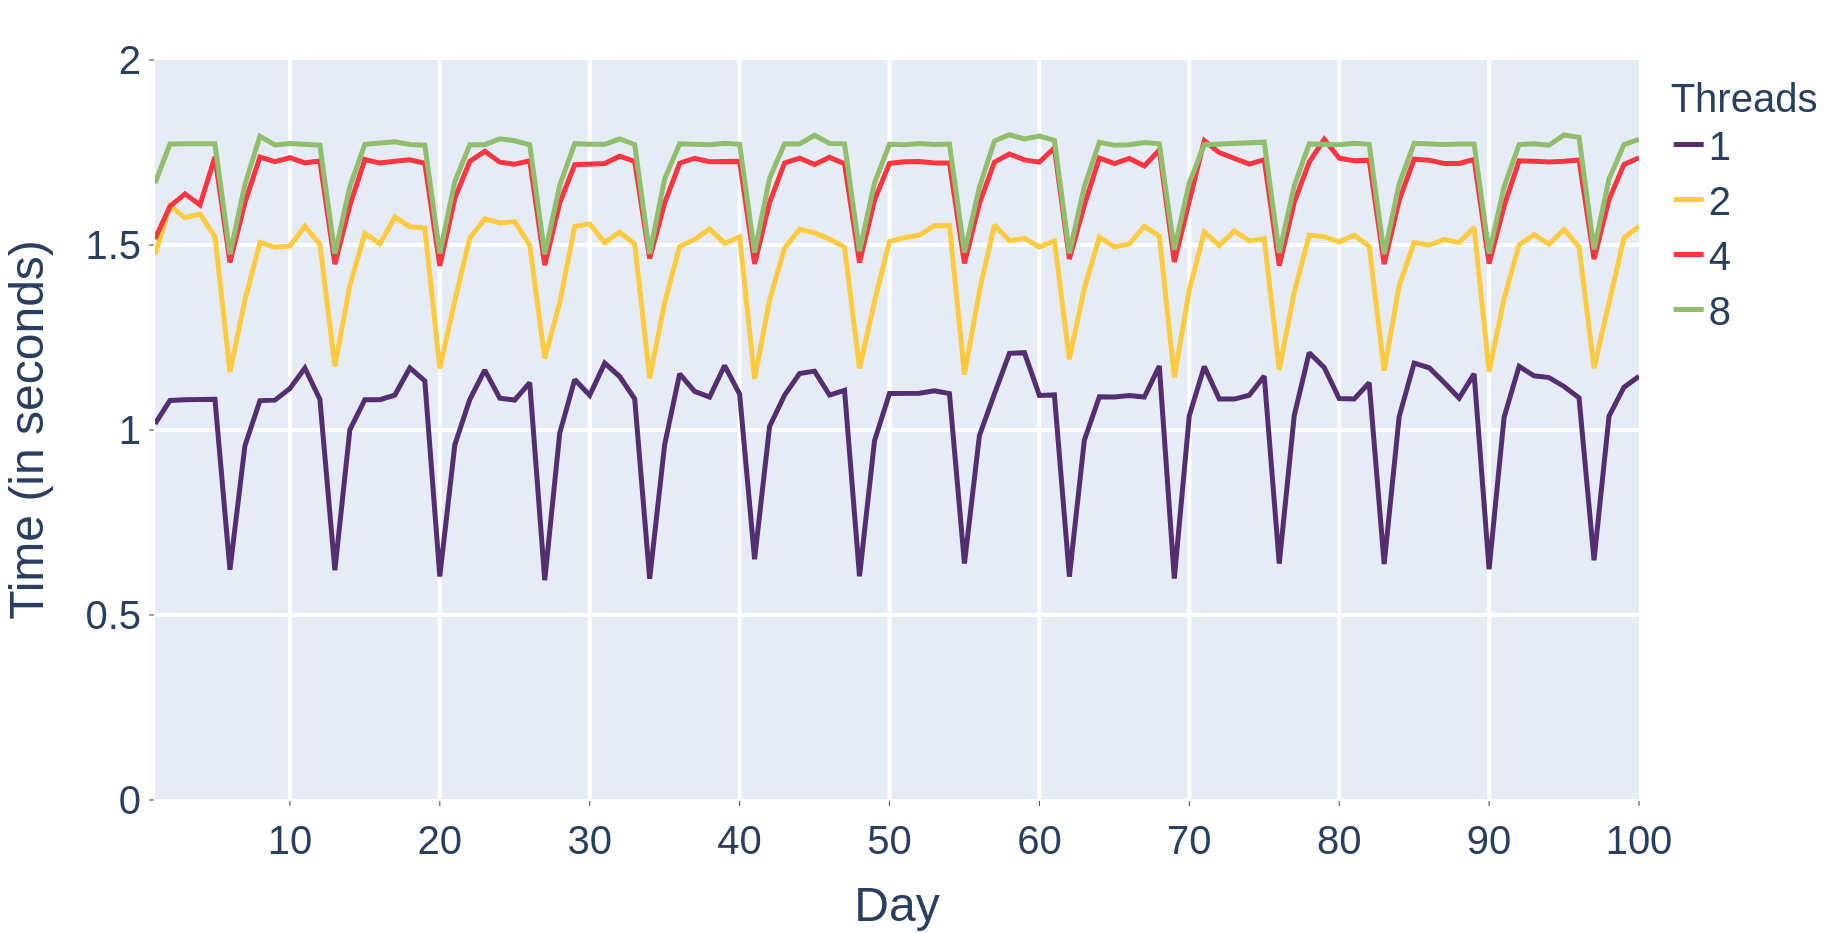
\includegraphics[width=\linewidth]{3 - Stride/fig/basis_parallel_updating.png}
    \caption{Time per simulation day for updating individuals using different number of threads. Simulations run on 11M population for 100 days without holidays (configurations in Appendix \ref{appendix:configurations}).}
    \label{fig:basis_parallel_updating}
\end{figure}

\begin{figure}
    \centering
    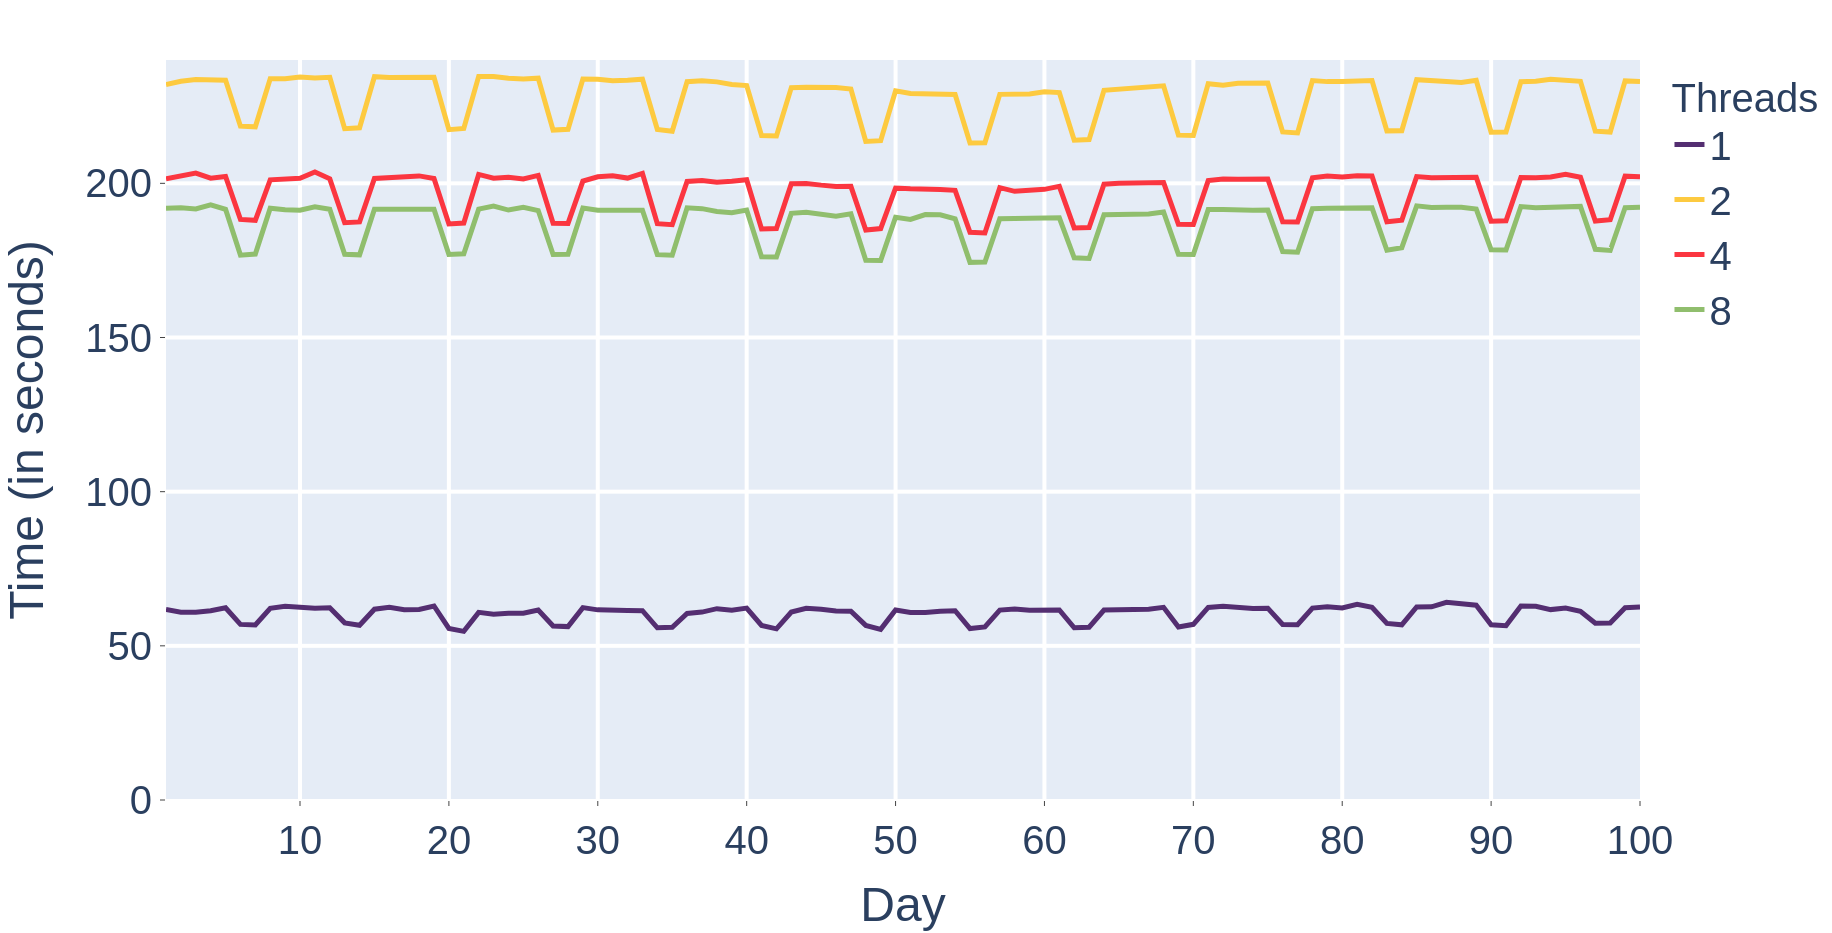
\includegraphics[width=\linewidth]{3 - Stride/fig/basis_all_parallel_infector.png}
    \caption{Time per simulation day for the infector using \textsc{All-to-All} using different number of threads. Simulations run on 11M population for 100 days without holidays (configurations in Appendix \ref{appendix:configurations}).}
    \label{fig:basis_all_parallel_infector}
\end{figure}

\begin{figure}
    \centering
    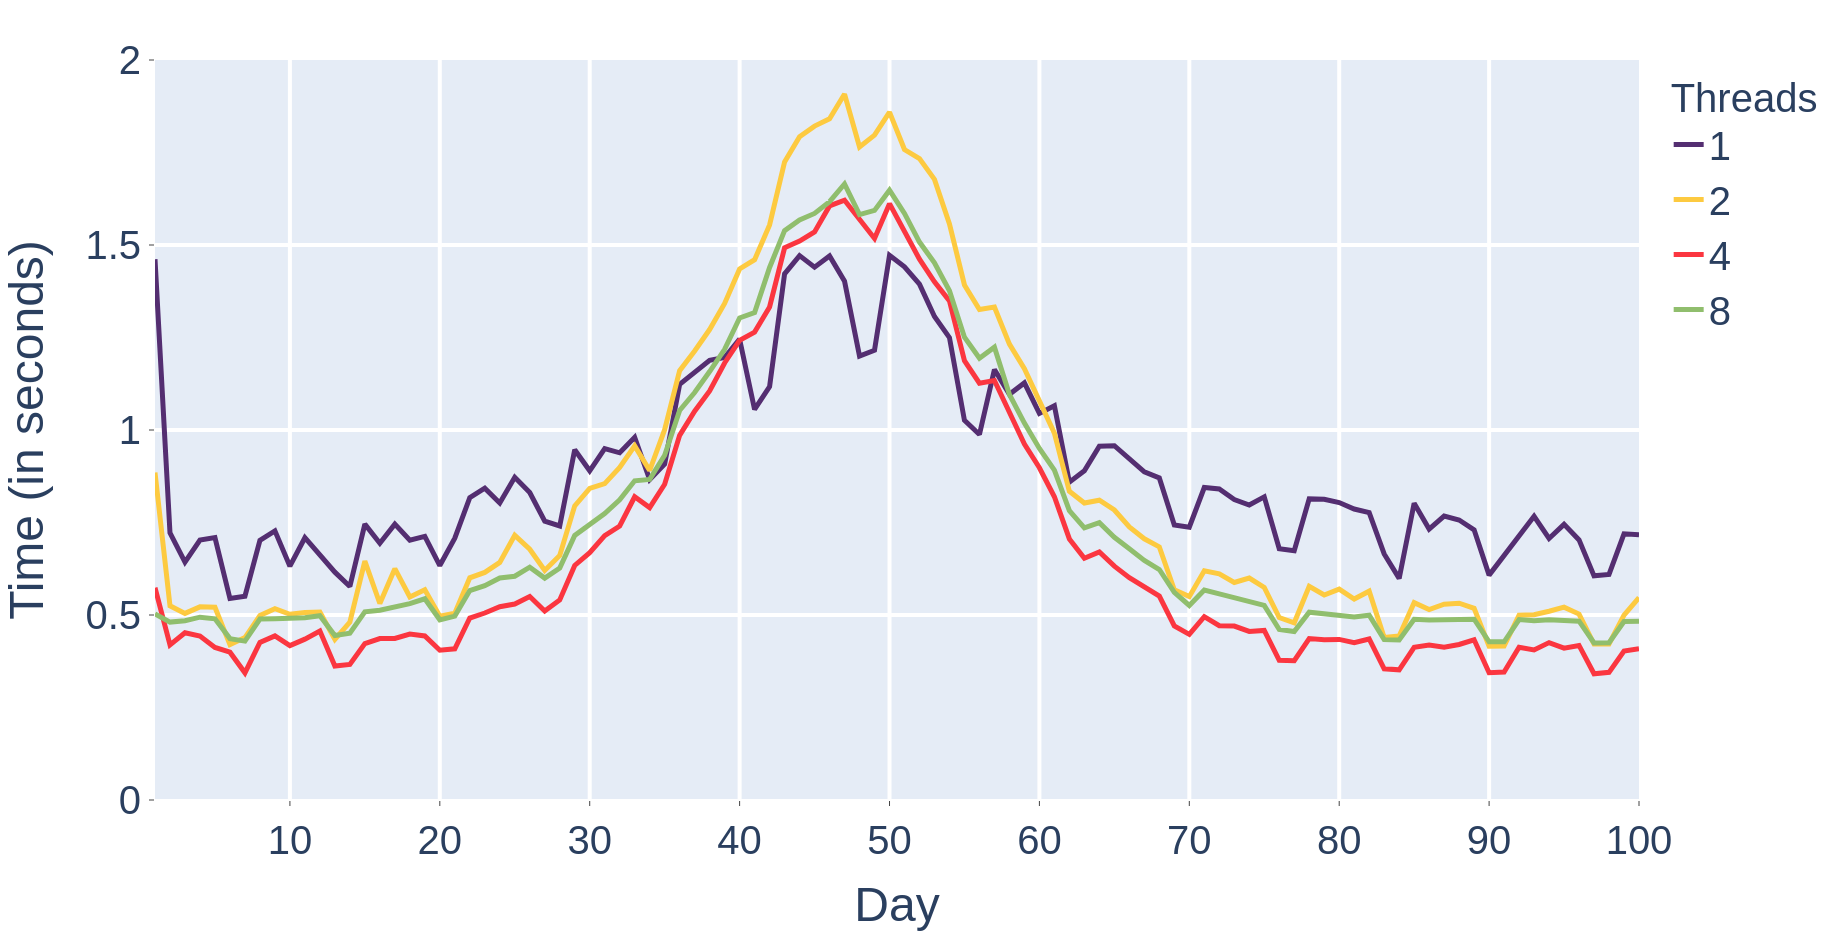
\includegraphics[width=\linewidth]{3 - Stride/fig/basis_opt_parallel_infector.png}
    \caption{Time per simulation day for the infector using \textsc{Inf-to-Sus} using different number of threads. Simulations run on 11M population for 100 days without holidays (configurations in Appendix \ref{appendix:configurations}).}
    \label{fig:basis_opt_parallel_infector}
\end{figure}

\begin{table}
    \begin{subtable}[h]{0.45\textwidth}
        \centering
        \begin{tabular}{@{}crrr@{}}
            \toprule
            Threads & Updating & Infector & Total  \\ \midrule
            1       & 1.08     & 64.33    & 65.56  \\
            2       & 1.45     & 227.93   & 229.50 \\
            4       & 1.67     & 197.04   & 198.85 \\
            8       & 1.72     & 187.15   & 189.00 \\ \bottomrule
        \end{tabular}
        \caption{\textsc{All-to-All}.}
        \label{tab:basis_all_parallel}
    \end{subtable}
    \hfill
    \begin{subtable}[h]{0.45\textwidth}
        \centering
        \begin{tabular}{@{}crrr@{}}
            \toprule
            Threads & Updating & Infector & Total \\ \midrule
            1       & 1.10     & 0.89     & 2.12  \\
            2       & 1.52     & 0.83     & 2.48  \\
            4       & 1.66     & 0.69     & 2.49  \\
            8       & 1.67     & 0.75     & 2.57  \\ \bottomrule
        \end{tabular}
        \caption{\textsc{Inf-to-Sus}.}
        \label{tab:basis_opt_parallel}
    \end{subtable}
    \caption{Average daily runtime (in seconds) per section. Simulations run on 11M population for 100 days without holidays (configurations in Appendix \ref{appendix:configurations}).}
    \label{tab:basis_parallel}
\end{table}

\section{First optimisation}
\label{sec:first_optimisation}
In this section we examine the parallellization problem in depth and present our first major optimisation.

\subsection{Code architecture}
Before we go into details about Stride, we need to disclose the architecture of the code. We will need this information when we need to contemplate about what causes these performance issues.

\subsubsection{Population}
Representing 11 million individuals is, needless to say, a lot of data that has to be stored and managed. Stride uses a segmented vector for its population, which is a container that stores objects, which are individuals in our case, almost contiguously in a chain of blocks. The block size, which is set to 2048, determines how many individuals get stored consecutively. It is designed this way to have better performance regarding CPU caching.

\subsubsection{Person}
Every individual is represented in a \textit{Person} object. This object contains various information such as its ID and age, but also of which pools they are a member and in which they are currently present. Information about their health is stored in another \textit{Health} object. This health object stores the person's health status as well as their health characteristics.

\subsubsection{Shared pointer}
The \textit{Population} is wrapped in a \textit{std::shared\_ptr}. This is a smart pointer designed to facilitate the managing of storage of an object pointer when there are multiple owners that manage its lifetime \cite{shared_ptr_doc}. The underlying structure has a reference counter which keeps track of all instances of the shared pointer and deletes the memory source and itself when this counter reaches zero \cite{shared_ptr_doc_microsoft}.

\subsection{Updating individuals}
\label{subsec:first_opt_updating_individuals}
First we look at the updating of individuals, which needs more time to complete the more threads that are being used. In Sections \ref{subsec:health_status_update} and \ref{subsec:pool_presences} we discussed how every individual gets updated at the start of a simulation day regarding their health status and their pool presences. This is implemented with a single iteration over the entire population in which it calls the \textit{update} function of a Person. The examination of this code does not present any visible errors. A possible reason for the multithreading problem could be related to the memory management done by the CPU. If we want to solve this, there is a strong possibility that we need to do extensive research on this topic and maybe redesign a great portion of the code, which lies outside the scope of this thesis. For this reason and because this section requires only a small portion of the total simulation time, we will ignore this section for now.
\\\\
Let it be stated that we only made assumptions here by looking at the code. We did not perform tests on this section because of the little impact it would have on the total runtime. There is always the possibility to turn of the multithreading for this section, which would still result in acceptable runtimes.

\subsection{Infector}
\label{subsec:first_opt_infector}
We learned that it costs substantially more time for the infector when we use multiple threads and that the \textsc{Inf-to-Sus} infector displays a strange phenomenon, as seen in Figure \ref{fig:basis_opt_parallel_infector}, where multithreading can be both faster and slower depending on the day. We already said that the curve of the \textsc{Inf-to-Sus} infector graph is connected to the number of people who are infected. When there are only a few infected people, the infector from Algorithm \ref{alg:inf-to-sus} then can skip a lot of pools that do not contain an infected member. When multiple threads are being used in the days with a few infections, the infector for \textsc{Inf-to-Sus} is faster than without multithreading. For these reasons we can conclude that the parallellization with OpenMP works well to distribute the infector calls amongst the threads, as seen in Algorithm \ref{alg:infector}, and that the fault probably lies in the \textsc{Inf-to-Sus} code.

\subsection{Solution}
\label{subsec:first_opt_solution}
After detailed examination of both infector algorithms and performing tests, we noticed that most of the infector time was spent for calculating the contact probabilities. When we looked at the code for this function, for which the pseudo code is shown in Algorithm \ref{alg:contact_probability}, we noticed that the population is also a parameter. The reason that this function costs so much time, was because the \textit{shared\_ptr} of this population was being passed by value. In C++, when a parameter is passed by value, a copy of that parameter is created in memory and passed on instead of the original. This is useful when we want to make sure that the function does not change the original data. However, this means that in our case a copy of the \textit{shared\_ptr} of the population needs to be created every time we want to calculate a contact probability. Let it be clear that this is not the same as copying the population itself, but only the \textit{shared\_ptr}.
\\\\
A copy of a normal pointer in C++ would not cause much trouble, because it is only a reference number to the data it points to. When a \textit{shared\_ptr} or a copy of it gets created or destroyed, the reference counter of the shared pointer needs to be updated, which causes some overhead \cite{shared_ptr_doc_microsoft}. The calculation of the contact probability is called for every pair of individuals in \textsc{All-to-All} and for every infectious and susceptible pair in \textsc{Inf-to-Sus} in a pool. Since there is a gigantic amount of pools that need to be passed on to infector, this results in innumerous contact probabilities that need to be calculated and thus results in a lot of overhead. A secondary issue is that the updating of the \textit{shared\_ptr} reference counter is an atomic operation, which means that when a thread needs to update it, it blocks other blocks from accessing this reference counter. Because of this, all the other threads have to wait their turn so that they can update the counter before continuing their thread of execution. This means that there is even more overhead when we use multiple threads for the infector \cite{shared_ptr_doc_microsoft}.
% https://stackoverflow.com/questions/22295665/how-much-is-the-overhead-of-smart-pointers-compared-to-normal-pointers-in-c
\\\\
The solution for all of this is to change the code so that the \textit{shared\_ptr} population is passed by reference instead of by value. This will only create a reference to the shared pointer instead of creating a new one. When a value is passed by reference, the function that gets called then has the power to change the original value, so we need to be cautious when we do this. Because of this, we examined the code of the contact probability function and saw that there were only read operations on the population data, so we can safely say that our changes will not result in malicious code.

\subsection{Results}
The changes that we made only affect the infector and the total runtime. The comparisons between the original version and our solution without multithreading is shown in Figure \ref{fig:basis_standard_comparison}. Figure \ref{fig:basis_standard_comparison_all} shows us that the infector and total runtime of \textsc{All-to-All} is now almost twice as fast with our change than before. \textsc{Inf-to-Sus} only shows a small increase in speed in Figure \ref{fig:basis_standard_comparison_opt}. The results in Table \ref{tab:basis_standard} confirm that we achieve an average total speedup per simulation day of 1.82 and 1.04 when using respectively \textsc{All-to-All} and \textsc{Inf-to-Sus}. Figure \ref{fig:standard_sections} visualizes the new ratios of the sections of the optimised Stride simulations using \textsc{All-to-All} and \textsc{Inf-to-Sus}. The averages of the sections are displayed in Table \ref{tab:standard_sections}. \textsc{All-to-All} spends significantly less time in infector than before, while the differences in speed for \textsc{Inf-to-Sus} are very little.
\\\\
We stated that multithreading would benefit even more if we pass the \textit{shared\_ptr} population by reference instead of by value. Figure \ref{fig:standard_parallel_infector} proves that we were correct and that we can now get better times with parallellization. In Table \ref{tab:basis_standard_parallel} we see that the speedups for \textsc{All-to-All} become larger the more threads that are being used. Although we improved Stride considerably, there is still a problem with \textsc{All-to-All} multithreading. Using eight threads on \textsc{Inf-to-Sus} is also slower than four. These issues might all have to do something with the memory, as mentioned before. We will focus from now on only on using Stride with only thread.

\begin{figure}
    \centering
    \begin{subfigure}[b]{\linewidth}
        \centering
        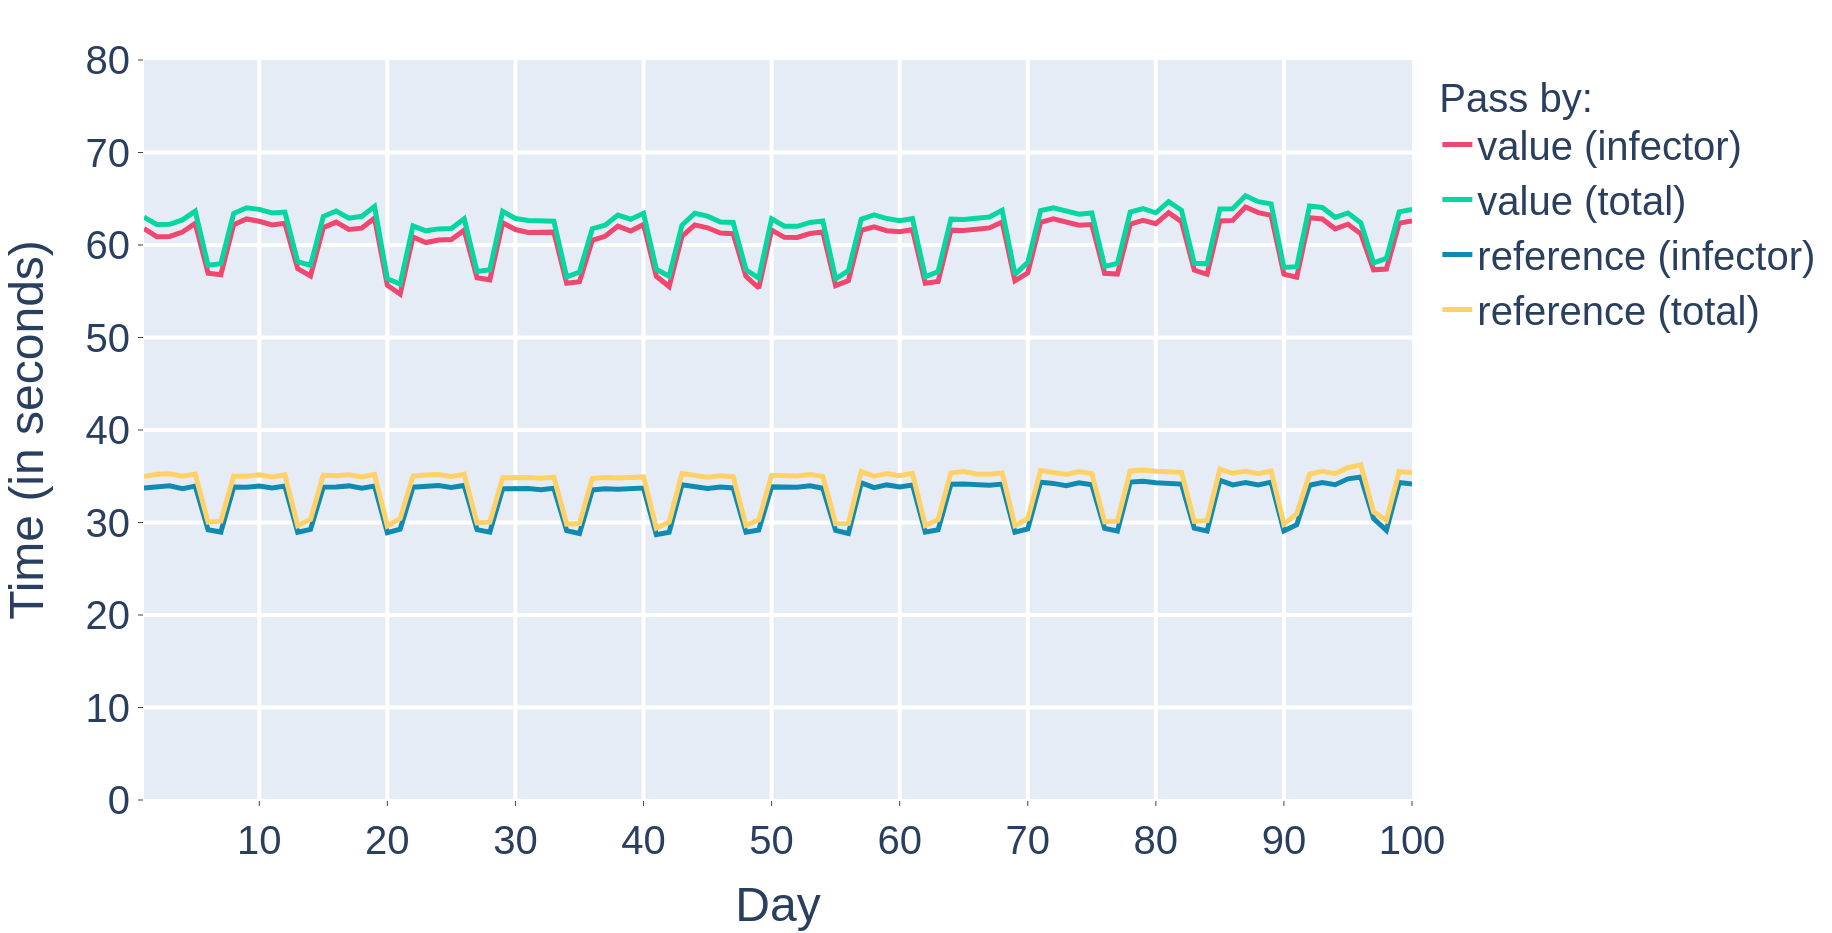
\includegraphics[width=\linewidth]{3 - Stride/fig/basis_standard_comparison_all.png}
        \caption{\textsc{All-to-All}}
        \label{fig:basis_standard_comparison_all}
    \end{subfigure}
    \begin{subfigure}[b]{\linewidth}
        \centering
        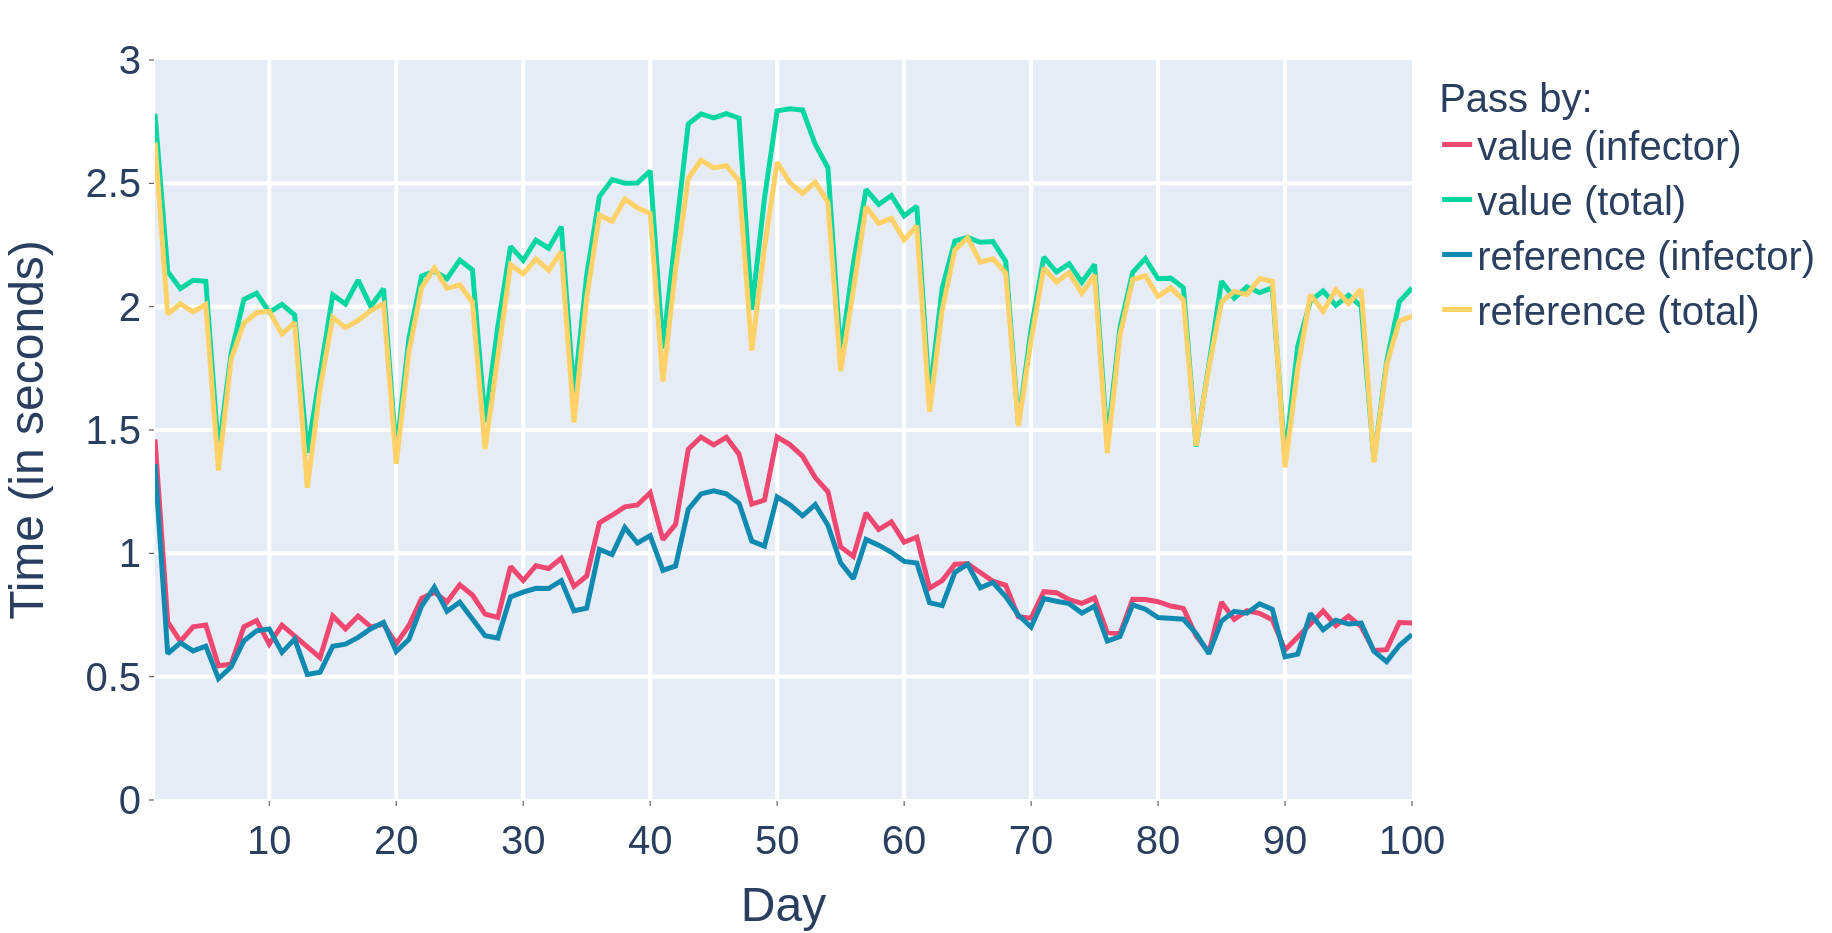
\includegraphics[width=\linewidth]{3 - Stride/fig/basis_standard_comparison_opt.png}
        \caption{\textsc{Inf-to-Sus}.}
        \label{fig:basis_standard_comparison_opt}
    \end{subfigure}
    \caption{Comparison of the infector and total runtimes of passing the population by value and by reference without parallellization. Simulations run on 11M population for 100 days without holidays using 1 thread (configurations in Appendix \ref{appendix:configurations}).}
    \label{fig:basis_standard_comparison}
\end{figure}

\begin{figure}
    \centering
    \begin{subfigure}[b]{\linewidth}
        \centering
        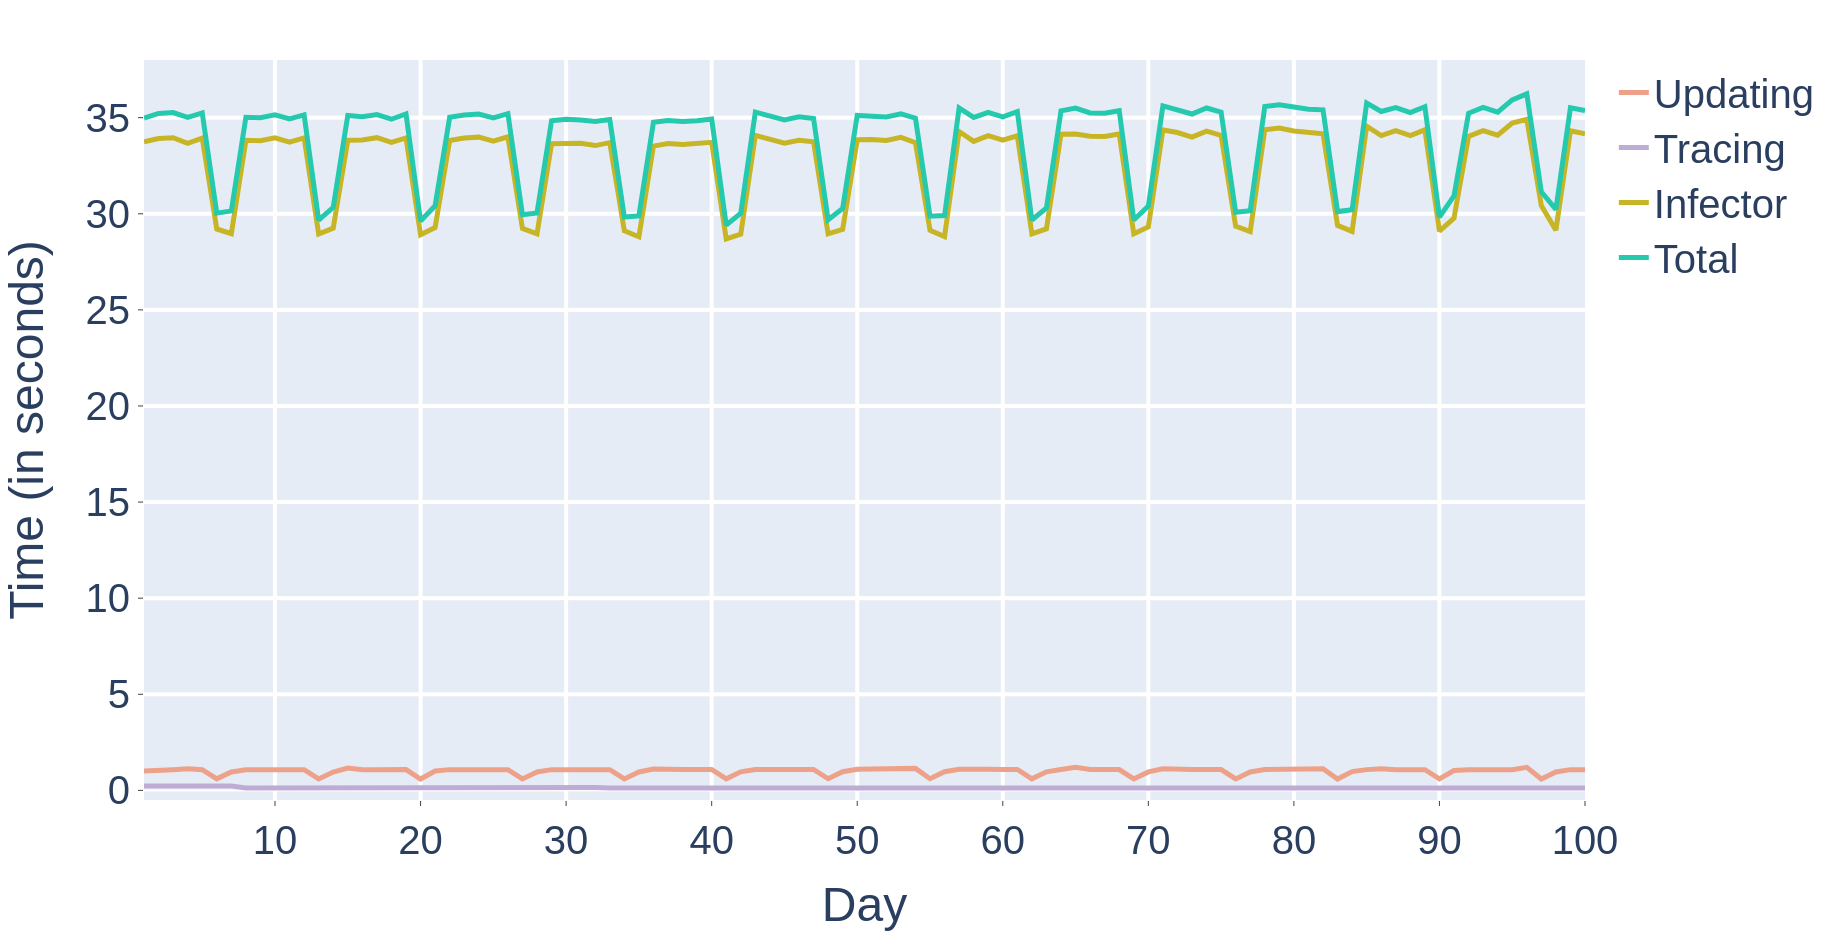
\includegraphics[width=\linewidth]{3 - Stride/fig/standard_all_runtime_sections.png}
        \caption{\textsc{All-to-All}}
        \label{fig:standard_all_sections}
    \end{subfigure}
    \begin{subfigure}[b]{\linewidth}
        \centering
        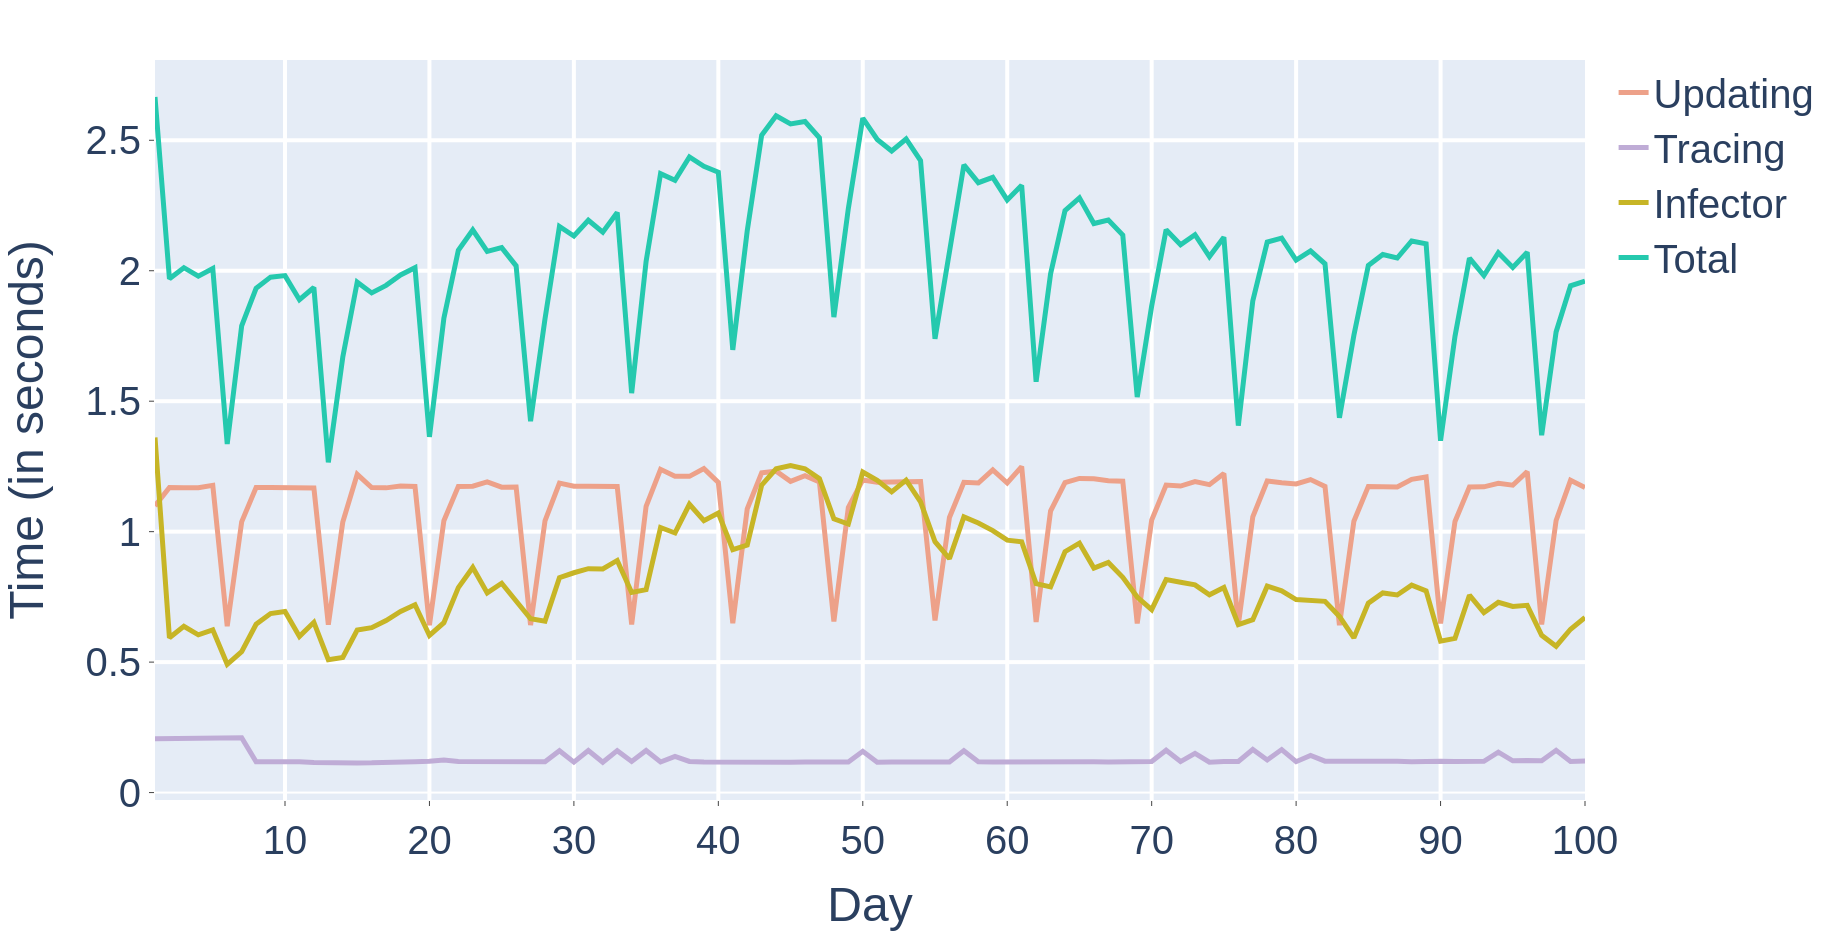
\includegraphics[width=\linewidth]{3 - Stride/fig/standard_opt_runtime_sections.png}
        \caption{\textsc{Inf-to-Sus}.}
        \label{fig:standard_opt_sections}
    \end{subfigure}
    \caption{Section times per day, in seconds, for every section, including the total times for simulating a day using the pass by reference optimisation. Simulations run on 11M population for 100 days without holidays using 1 thread (configurations in Appendix \ref{appendix:configurations}).}
    \label{fig:standard_sections}
\end{figure}

\begin{figure}
    \centering
    \begin{subfigure}[b]{\linewidth}
        \centering
        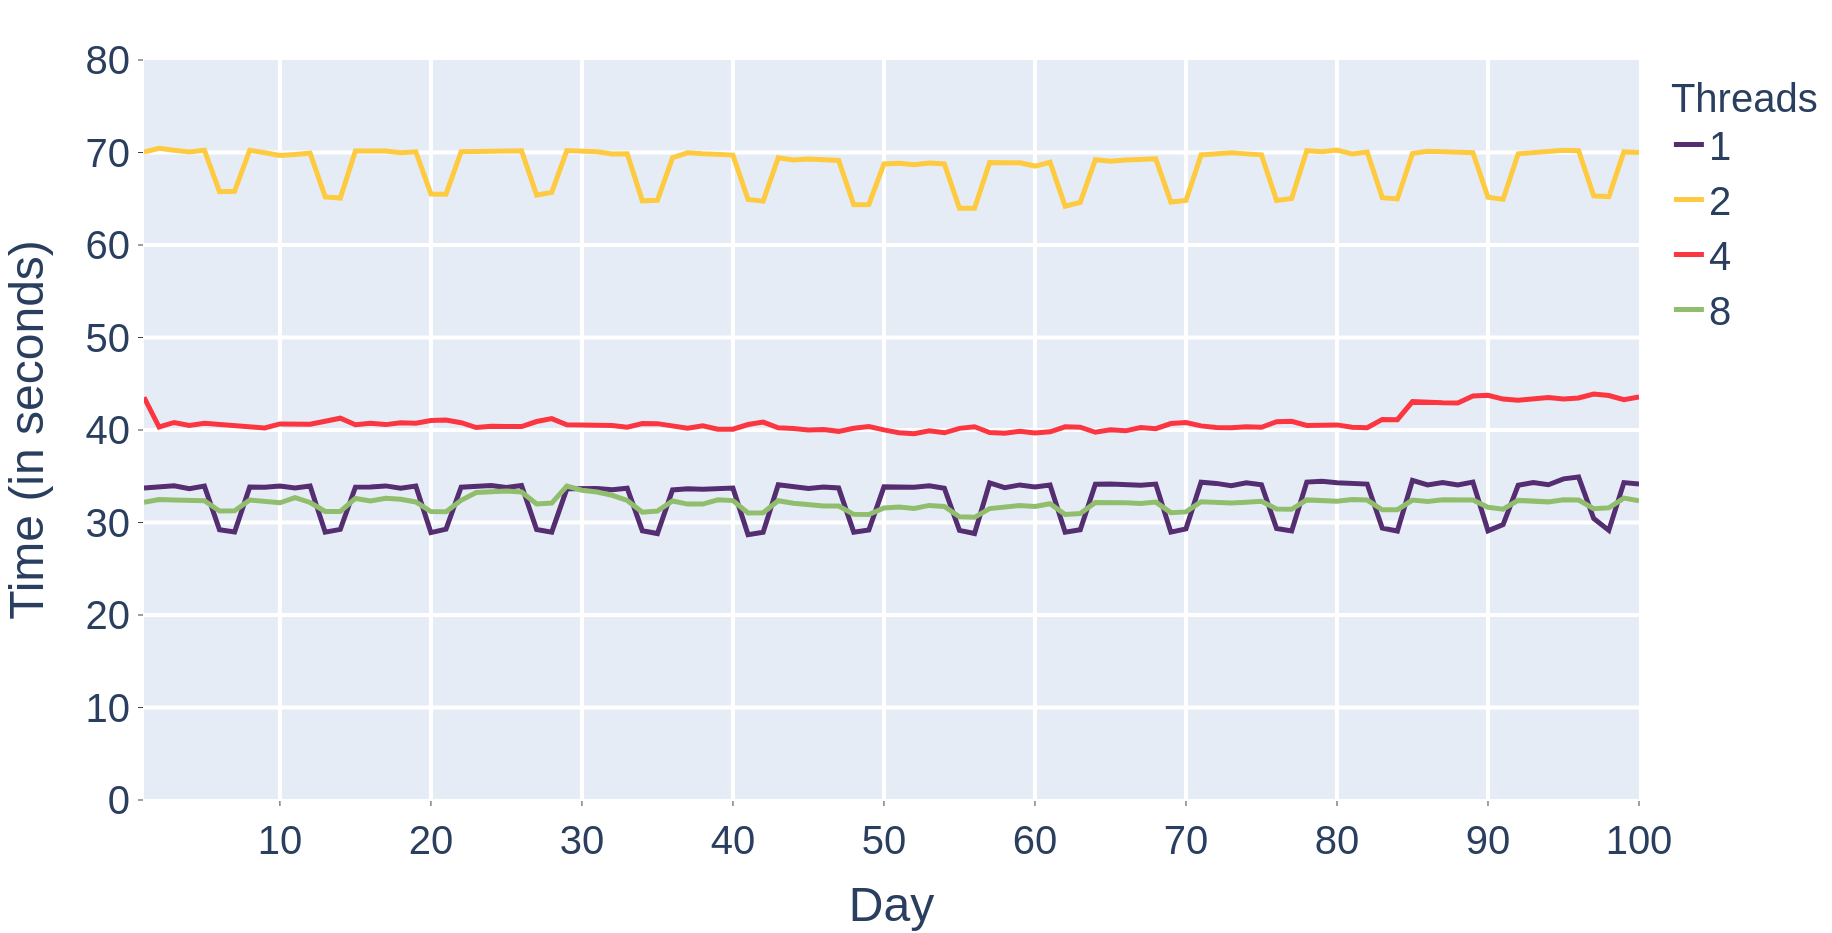
\includegraphics[width=\linewidth]{3 - Stride/fig/standard_all_parallel_infector.png}
        \caption{\textsc{All-to-All}}
        \label{fig:standard_all_parallel_infector}
    \end{subfigure}
    \begin{subfigure}[b]{\linewidth}
        \centering
        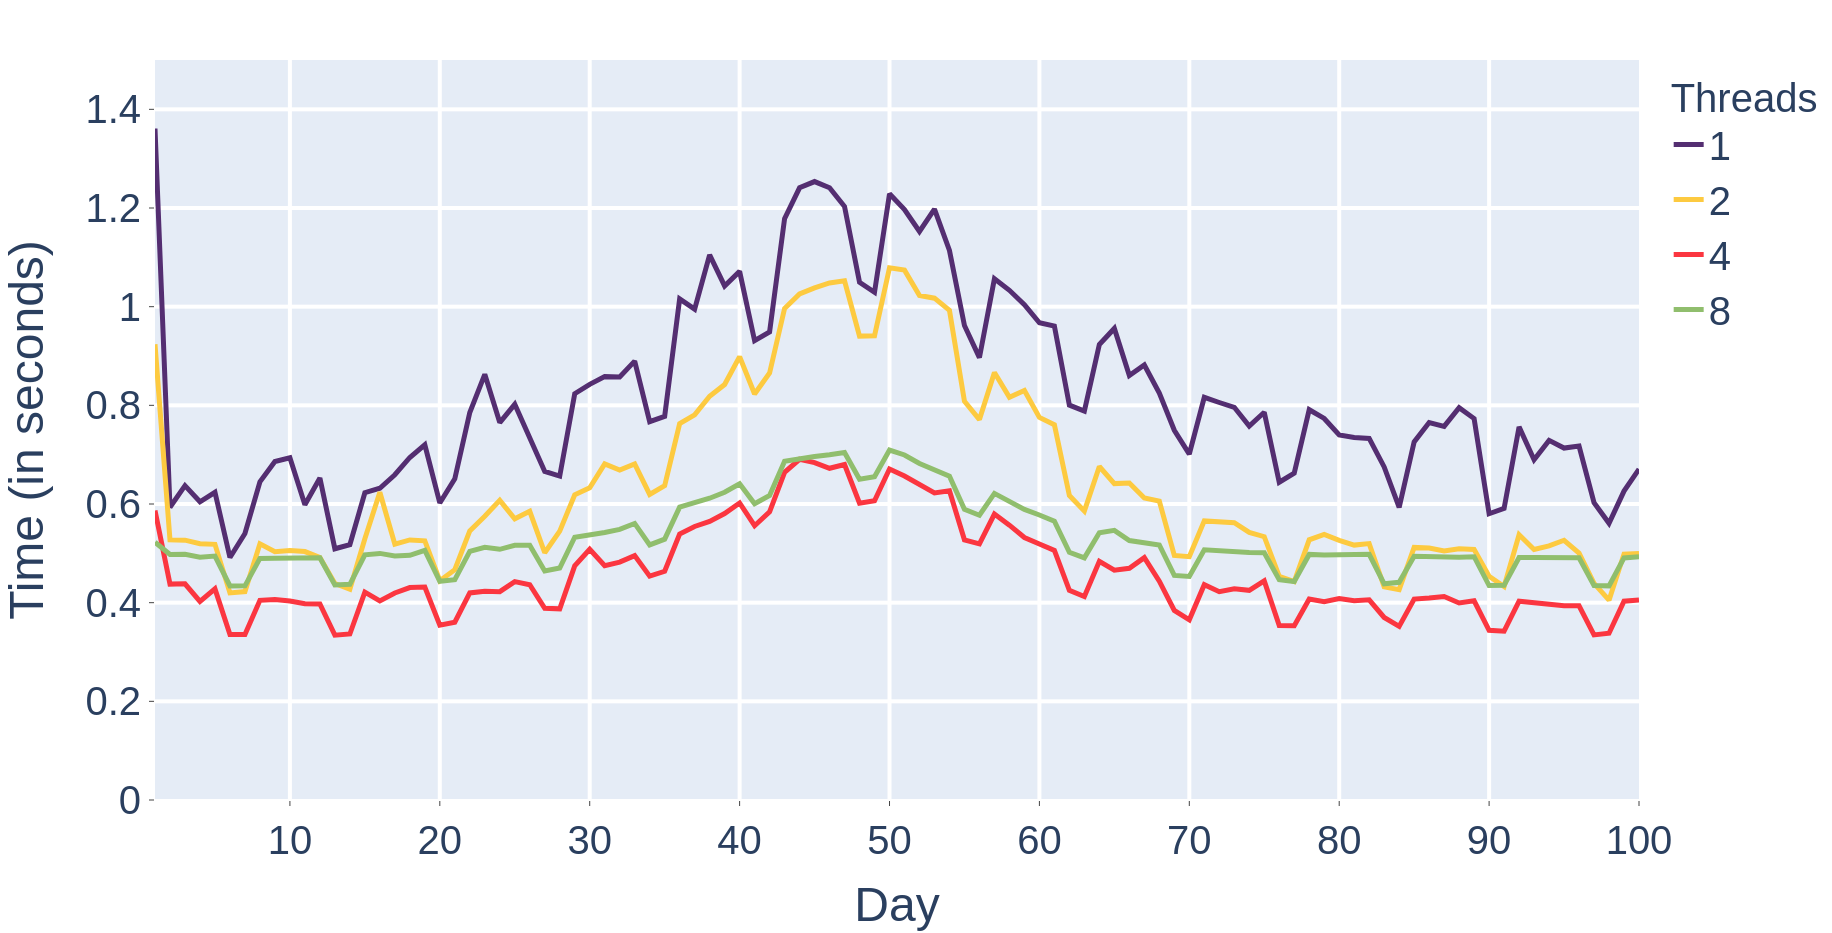
\includegraphics[width=\linewidth]{3 - Stride/fig/standard_opt_parallel_infector.png}
        \caption{\textsc{Inf-to-Sus}.}
        \label{fig:standard_opt_parallel_infector}
    \end{subfigure}
    \caption{Time per day for the infector that passes the $shared\_ptr$ population by reference, using different number of threads. Simulations run on 11M population for 100 days without holidays using 1 thread (configurations in Appendix \ref{appendix:configurations}).}
    \label{fig:standard_parallel_infector}
\end{figure}

\begin{table}[!ht]
    \begin{subtable}[h]{0.45\textwidth}
        \centering
        \begin{tabular}{@{}lrr@{}}
            \toprule
             & Infector & Total \\ \midrule
            pass by value & 60.37 & 61.52 \\
            pass by reference & 32.63 & 33.77 \\ \hdashline[1pt/1pt]
            speedup & 1.85 & 1.82 \\ \bottomrule
        \end{tabular}
        \caption{\textsc{All-to-All}}
        \label{tab:basis_standard_all}
    \end{subtable}
    \hfill
    \begin{subtable}[h]{0.45\textwidth}
        \centering
        \begin{tabular}{@{}lrr@{}}
            \toprule
             & Infector & Total \\ \midrule
            pass by value & 0.89 & 2.12 \\
            pass by reference & 0.82 & 2.04 \\ \hdashline[1pt/1pt]
            speedup & 1.09 & 1.04 \\ \bottomrule
        \end{tabular}
        \caption{\textsc{Inf-to-Sus}.}
        \label{tab:basis_standard_opt}
    \end{subtable}
    \caption{Average daily runtime (in seconds) per section of Stride before and after the optimisation with passing by reference. Simulations run on 11M population for 100 days without holidays using 1 thread (configurations in Appendix \ref{appendix:configurations}).}
    \label{tab:basis_standard}
\end{table}

\begin{table}[!ht]
\centering
\begin{tabular}{@{}lrrrr@{}}
\toprule
 & Updating & Tracing & Infector & Total \\ \midrule
All-to-All & 1.01 & 0.13 & 32.63 & 33.77 \\
Inf-to-Sus & 1.09 & 0.13 & 0.82 & 2.04 \\ \bottomrule
\end{tabular}
\caption{Average daily runtime (in seconds) per section of Stride with the passing by reference optimisation. Simulations run on 11M population for 100 days without holidays using 1 thread (configurations in Appendix \ref{appendix:configurations}).}
\label{tab:standard_sections}
\end{table}

\begin{table}[!ht]
    \begin{subtable}[h]{0.45\textwidth}
        \centering
        \begin{tabular}{@{}clrr@{}}
            \toprule
            Threads & Method & Infector & Total \\ \midrule
            \multirow{2}{*}{1} & by value & 60.37 & 61.52 \\
             & by reference & 32.63 & 33.77 \\ \hdashline[1pt/1pt]
             & speedup & 1.85 & 1.82 \\ \midrule
            \multirow{2}{*}{2} & by value & 227.93 & 229.50 \\
             & by reference & 68.40 & 70.13 \\ \hdashline[1pt/1pt]
             & speedup & 3.33 & 3.27 \\ \midrule
            \multirow{2}{*}{4} & by value & 197.04 & 198.85 \\
             & by reference & 40.91 & 42.68 \\ \hdashline[1pt/1pt]
             & speedup & 4.82 & 4.66 \\ \midrule
            \multirow{2}{*}{8} & by value & 187.15 & 189.00 \\
             & by reference & 32.03 & 33.82 \\ \hdashline[1pt/1pt]
             & speedup & 5.84 & 5.89 \\ \bottomrule
        \end{tabular}
    \caption{\textsc{All-to-All}}
    \label{tab:basis_standard_parallel_all}
    \end{subtable}
    \hfill
    \begin{subtable}[h]{0.45\textwidth}
        \centering
        \begin{tabular}{@{}clrr@{}}
            \toprule
            Threads & Method & Infector & Total \\ \midrule
            \multirow{2}{*}{1} & by value & 0.89 & 2.12 \\
             & by reference & 0.82 & 2.04 \\ \hdashline[1pt/1pt]
             & speedup & 1.09 & 1.04 \\ \midrule
            \multirow{2}{*}{2} & by value & 0.83 & 2.48 \\
             & by reference & 0.63 & 2.43 \\ \hdashline[1pt/1pt]
             & speedup & 1.32 & 1.02 \\ \midrule
            \multirow{2}{*}{4} & by value & 0.69 & 2.49 \\
             & by reference & 0.46 & 2.24 \\ \hdashline[1pt/1pt]
             & speedup & 1.50 & 1.11 \\ \midrule
            \multirow{2}{*}{8} & by value & 0.76 & 2.57 \\
             & by reference & 0.53 & 2.33 \\ \hdashline[1pt/1pt]
             & speedup & 1.43 & 1.10 \\ \bottomrule
        \end{tabular}
        \caption{\textsc{Inf-to-Sus}.}
        \label{tab:basis_standard_parallel_opt}
    \end{subtable}
    \caption{Comparison of the average daily runtimes (in seconds) per section before and after the pass by reference optimisation, depending on the number of used threads.  Simulations run on 11M population for 100 days without holidays (configurations in Appendix \ref{appendix:configurations}).}
    \label{tab:basis_standard_parallel}
\end{table}
\chapter{Sampling}
\label{chapter:sampling}
The optimised version of Stride from the previous chapter will be our new standard from now on. We also discussed that the most room for improvement lies in the infector algorithm of our model when using \textsc{All-to-All} and that we primarily focus on Stride without parallellization. Our previous optimisation was the result of a solution for an implementation issue, for which programming expertise is required to notice and solve it. This chapter presents an improvement by redesigning the infector algorithm, which requires less detailed programming knowledge to understand.

\section{General idea}
\label{sec:general_idea}
We learned that the \textsc{All-to-All} algorithm calculates contacts and transmissions in a contact pool, by comparing every individual with every other individual inside the pool. Algorithm \ref{alg:all-to-all} showed that this is done with a double for-loop: iterate over the pool members and for every person in this iteration, also iterate over the remaining members. In computer science, when we want to indicate the time it takes for an algorithm or program to run, we use time complexity. This describes an estimation of the amount of operations that are performed. If we now consider the calculation of contact and transmission between two individuals as one operation, \textsc{All-to-All} has time complexity $\mathcal{O}(n^{2})$ with $n$ being the pool size. This means that the larger pools have a quadratic times bigger impact than the small ones. Of course these operations cost more time when there is contact than when there is not, but this gives us a general indication.

\begin{example}
\label{example:quadratic_complexity}
A pool with 10 people would need $10^{2} = 100$ operations, while a pool that consists of 100 people requires $100^{2} = 10,000$ operations.
\end{example}

\textsc{All-to-All} uses the double for-loop so it can compare every pair of individuals and determine if they have contact with each other and if they transmit the disease. The quadratic complexity of this algorithm is thus caused by the need to compare everyone with everyone inside a pool. When two people have contact, the model registers this and continues to calculate the transmission. If two people do not have contact, they are ignored and nothing happens or gets registered about the pair. These calculations can be seen as `wasted' time because they do not contribute anything to the simulation or results. The idea behind our optimisation is to minimize this wasted time by only doing the calculations that are necessary.
\\\\
Our approach to limit the useless calculations is by taking a random sample of the people in a pool for which an individual is guaranteed to have contact with. Then, we only compare the individual with the people in the sample to calculate transmissions. This algorithm would need to iterate over the pool members only once, which would result in time complexity $\mathcal{O}(n*k) \approx \mathcal{O}(n)$ with $n$ being the pool size and $k$ the sample size. It would thus in theory have a linear time complexity which is much more efficient than the original \textsc{All-to-All} with quadratic time complexity.
\\\\
In order for us to use this approach, we need a way to determine the sample sizes. Consider the \textsc{All-to-All} algorithm where we want to calculate the contacts for an individual. We loop over the pool members and calculate for every person if there is contact, which results in yes or no. If we now look at this from another point of view, every contact calculation is a Bernoulli trial that can result in a success or failure where the probability of success equals the contact probability \cite{bernoulli}. This means that for one individual the algorithm needs to compute multiple Bernoulli trials, which in turn can be seen as a binomial distribution for which the definition is the following \cite{binomial}:
\begin{quoting}
"The binomial distribution refers to the number of successes in $n$ independent trials with a common success probability $p$ in each."
\end{quoting}
\noindent This applies to our approach where $n$ is the number of people with whom we compare an individual and, as we already said, $p$ is the contact probability. Thus, if these two variables are known, we can calculate for an individual the sample size $k \sim Binomial(n, p)$. However, the issue with this is that the probability of two people having contact, is based on those two people. This means that we still would need to calculate the contact probability for every pair of individuals and be back to square one. The next sections will explain how we implemented our approach despite this obstacle.

\section{Preliminary insights}
\label{sec:preliminary_insights}
Before we start to discuss and evaluate improvements, we continue to examine the performance for the purpose of optimising the \textsc{All-to-All} infector. Therefore, the data, and figures in this section only contain results from Stride simulations using \textsc{All-to-All} without parallellization.

\subsection{Infector runtimes}
\label{subsec:infector_runtimes}
Since our focus lies on the \textsc{All-to-All} infector, it is in our best interest to fully understand how the infector has such a big impact as we saw in Section \ref{sec:first_optimisation}.

\subsubsection{Pool size runtimes}
In the previous section we explained how the original algorithm, in theory, should have a quadratic time complexity in function of the pool size. Figure \ref{fig:standard_times_all_averages} shows the average time per pool size the \textsc{All-to-All} algorithm needs for its calculations, where we can clearly see the quadratic curve that we talked about. Thus larger pool sizes have a much greater effect on the simulation time than the smaller ones. However, as we discussed in Section \ref{subsec:contact_pools_data}, there are far more pools that contain only a small amount of people.
\\\\
These average runtimes per pool size give us a representation of how the pool size affects the infector, but they do not illustrate the total infector runtimes in a simulation. In our general idea, we discussed an optimisation that becomes more effective the larger the pools. If, for example, the smaller pools take up much more time than the larger pools to calculate contacts and transmissions, our new method would be far less effective. There are almost five million households that consist of 1 to 6 persons, and 94\% of workplaces contain not more than nine people. Therefore, it could be possible that our optimisation has less effect, because there are vastly more small pools. In order to get insight into how our optimisations would affect the total simulation runtime, we want to know how the total infector runtime is distributed in function of the pool size. However, we cannot simply measure the runtimes for a day or even a full simulation, because pools are only active on specific days according to their contact pool type. Also, if we would just measure the infector runtimes of pools for a day on which they are active and add them all up, we would get a distorted representation. This is because primary communities are in general only active on weekend days, while secondary communities are only active on weekdays. The secondary communities have therefore a bigger impact on the total simulation runtime than primary ones. To give the most accurate representation, we measure seven consecutive days, without any holidays, so we get the total measurements of a `regular' week. At last, because Stride simulations are run per day and not per week, we divide these totals by seven to get a \textit{total daily average runtime}. This way, the primary and secondary communities, for example, have a total impact of respectively 2/7 and 5/7 times their total runtimes, because they are only active two and five out of seven days.
\\\\
Figure \ref{fig:standard_times_all_totals_weekly} shows these total daily average runtimes per pool size, where we can see the actual impact pool sizes have on the total simulation. Although the smaller pools do not spend a lot of time in the infector on their own, the total amount of time spent in the infector is comparable to larger sizes with far less pools. However, we can also see that smaller pools account for only a small percent of the total infector runtime, so we infer that our general idea will have a noticeable effect.

\begin{figure}
    \centering
    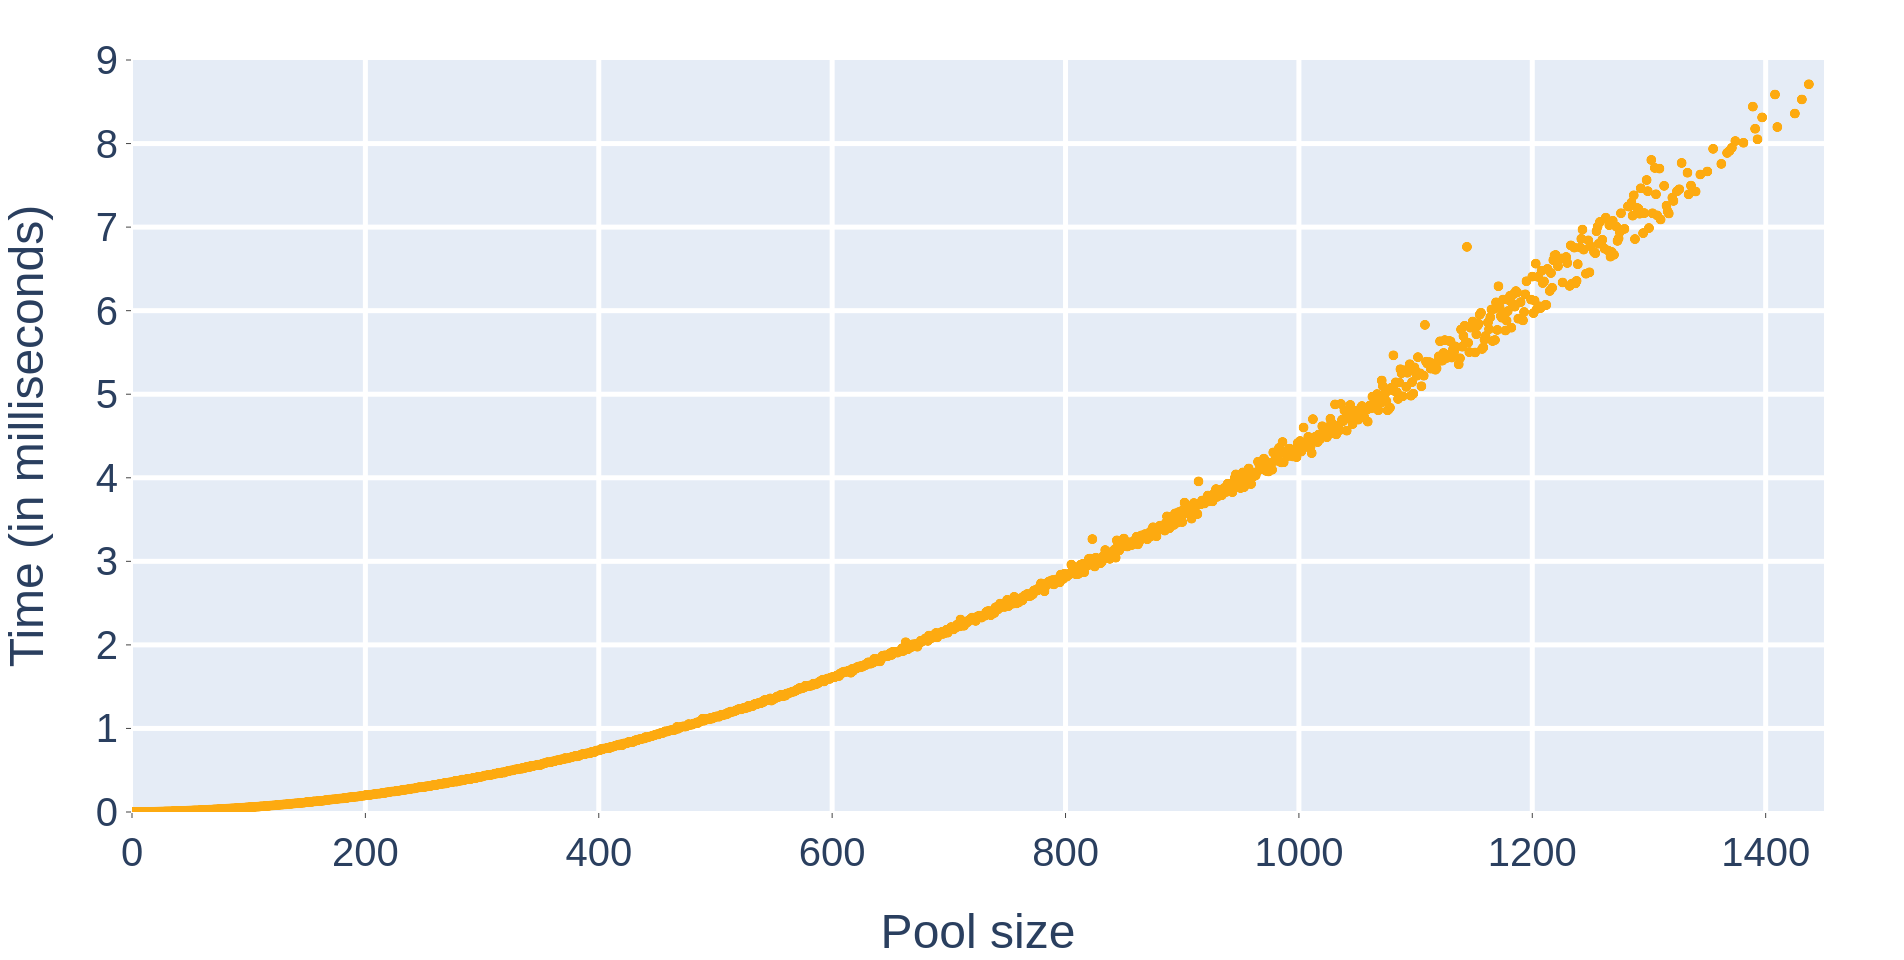
\includegraphics[width=\linewidth]{4 - Sampling/fig/standard/standard_times_all_averages.png}
    \caption{Average infector runtime (in milliseconds) per pool size using \textsc{All-to-All}. Simulation run on 11M population for 100 days without holidays using 1 thread (configurations in Appendix \ref{appendix:configurations}).}
    \label{fig:standard_times_all_averages}
\end{figure}

\begin{figure}
    \centering
    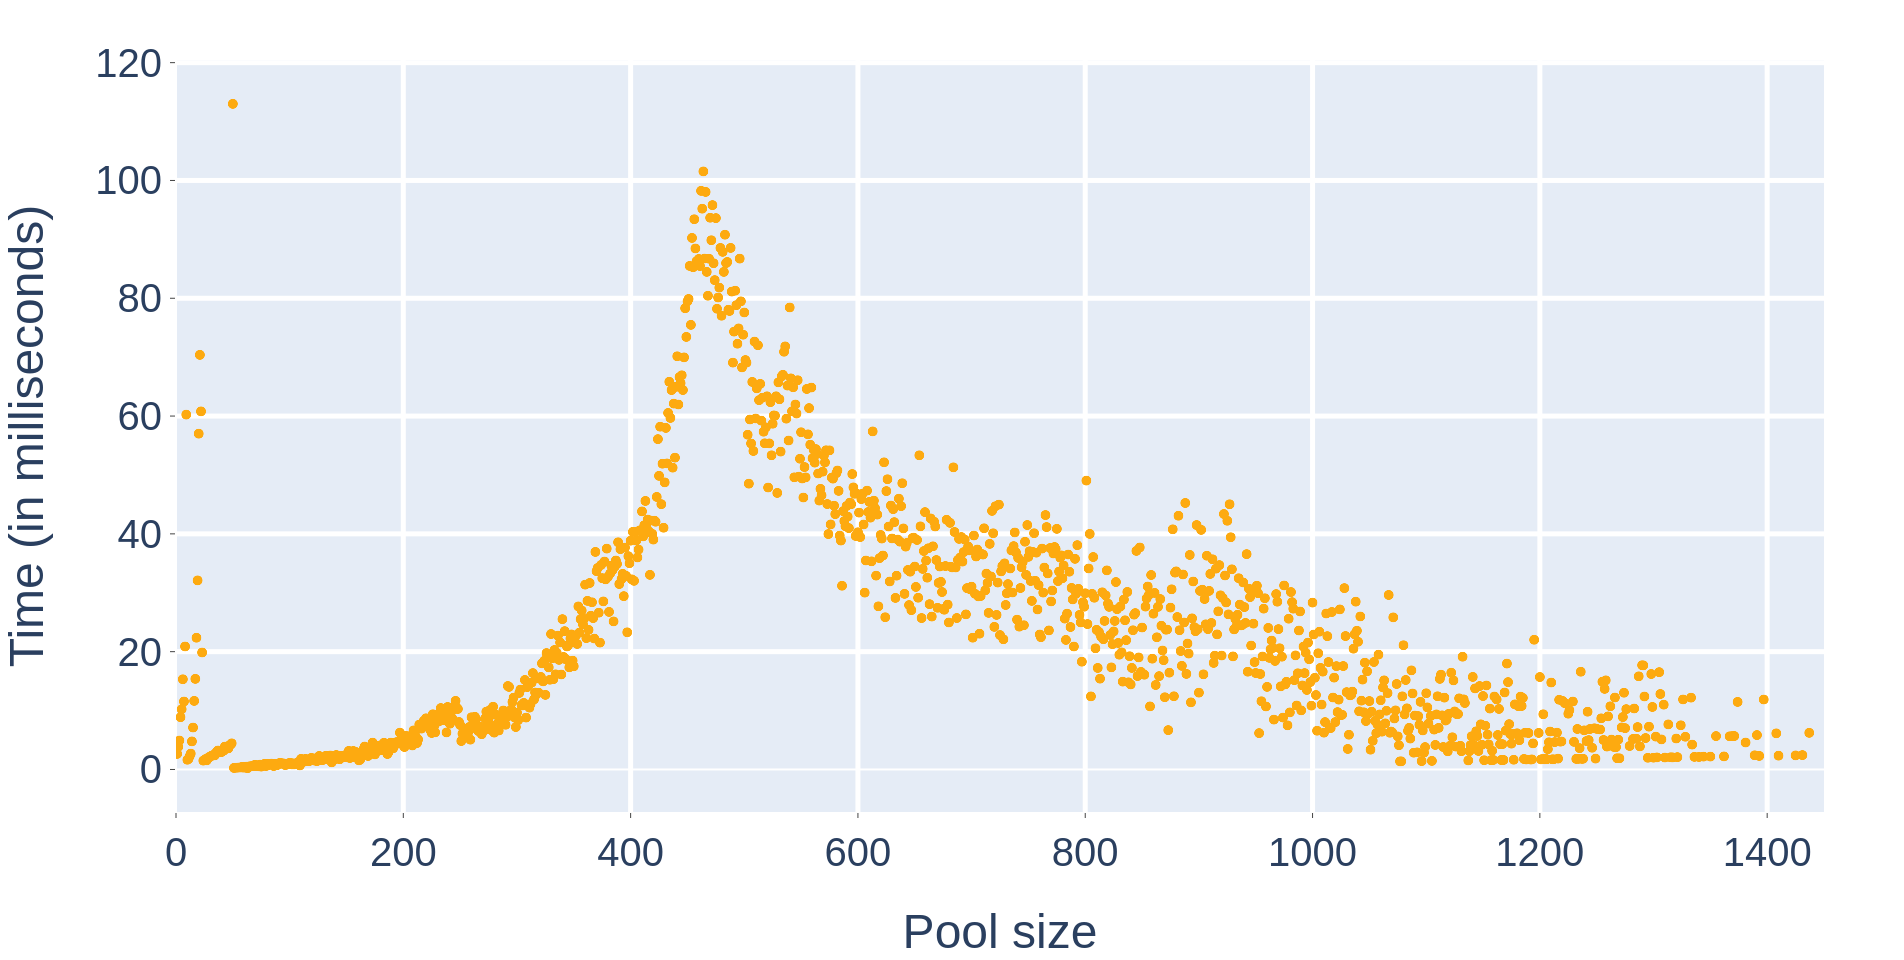
\includegraphics[width=\linewidth]{4 - Sampling/fig/standard/standard_times_all_totals_weekly.png}
    \caption{Total daily average infector runtime (in milliseconds) per pool size using \textsc{All-to-All}, based on a 7-day week. Simulation run on 11M population for 7 days without holidays using 1 thread (configurations in Appendix \ref{appendix:configurations}).}
    \label{fig:standard_times_all_totals_weekly}
\end{figure}

\subsubsection{Pool type runtimes}
Let it be noted that Figures \ref{fig:standard_times_all_averages} and \ref{fig:standard_times_all_totals_weekly} only present the results of measuring the time it takes for the \textsc{All-to-All} algorithm to calculate the contacts and transmissions for a pool with microsecond precision. The graph of Figure \ref{fig:standard_times_all_totals_weekly} reminds us of the pool size distributions of the primary and secondary community contact pools, which were discussed in Section \ref{subsec:contact_pools_data}, but we cannot say this with certainty. In order to get the most complete understanding of the infector runtimes, we also need to know how the different pool types influence the simulation runtime.
\\\\
Figure \ref{fig:standard_times_all_totals_weekly} displayed the total daily average runtimes in function of the pool size, but Figure \ref{fig:standard_times_type_totals} displays these results in function of the pool types and makes a distinction between two different measurements per pool type. \textit{Algorithm only} represents the total time spent in the infector algorithm for all the pools of a pool type. \textit{Total time} gives a more complete overview of the simulation time per pool type, by measuring the time it takes to iterate over all of the pools of a certain type and call infector on them. This distinction needs to be made, because otherwise we could get the wrong impressions of how the time is distributed. For example, all household pools combined only require 0.03 seconds in the algorithm, but it takes our model 1.72 seconds to iterate over every household to calculate their contacts and transmissions. This demonstrates that there is definitely some overhead that we cannot change, which is not surprising since Stride needs to iterate over almost five million households every day.
\\\\
What is most noteworthy about these results, are the proportions between the community pools and the rest. Both of them contain only 22,000 pools, but they account for the vast majority of the total infector runtime. This proves yet again that the larger pools are the main reason the simulation has suboptimal runtimes and that, in theory, our sampling approach will greatly improve this because of its linear time complexity. The difference between the primary and secondary community is due to the way we calculate the impact of every pool, which we previously explained.

\begin{figure}
    \centering
    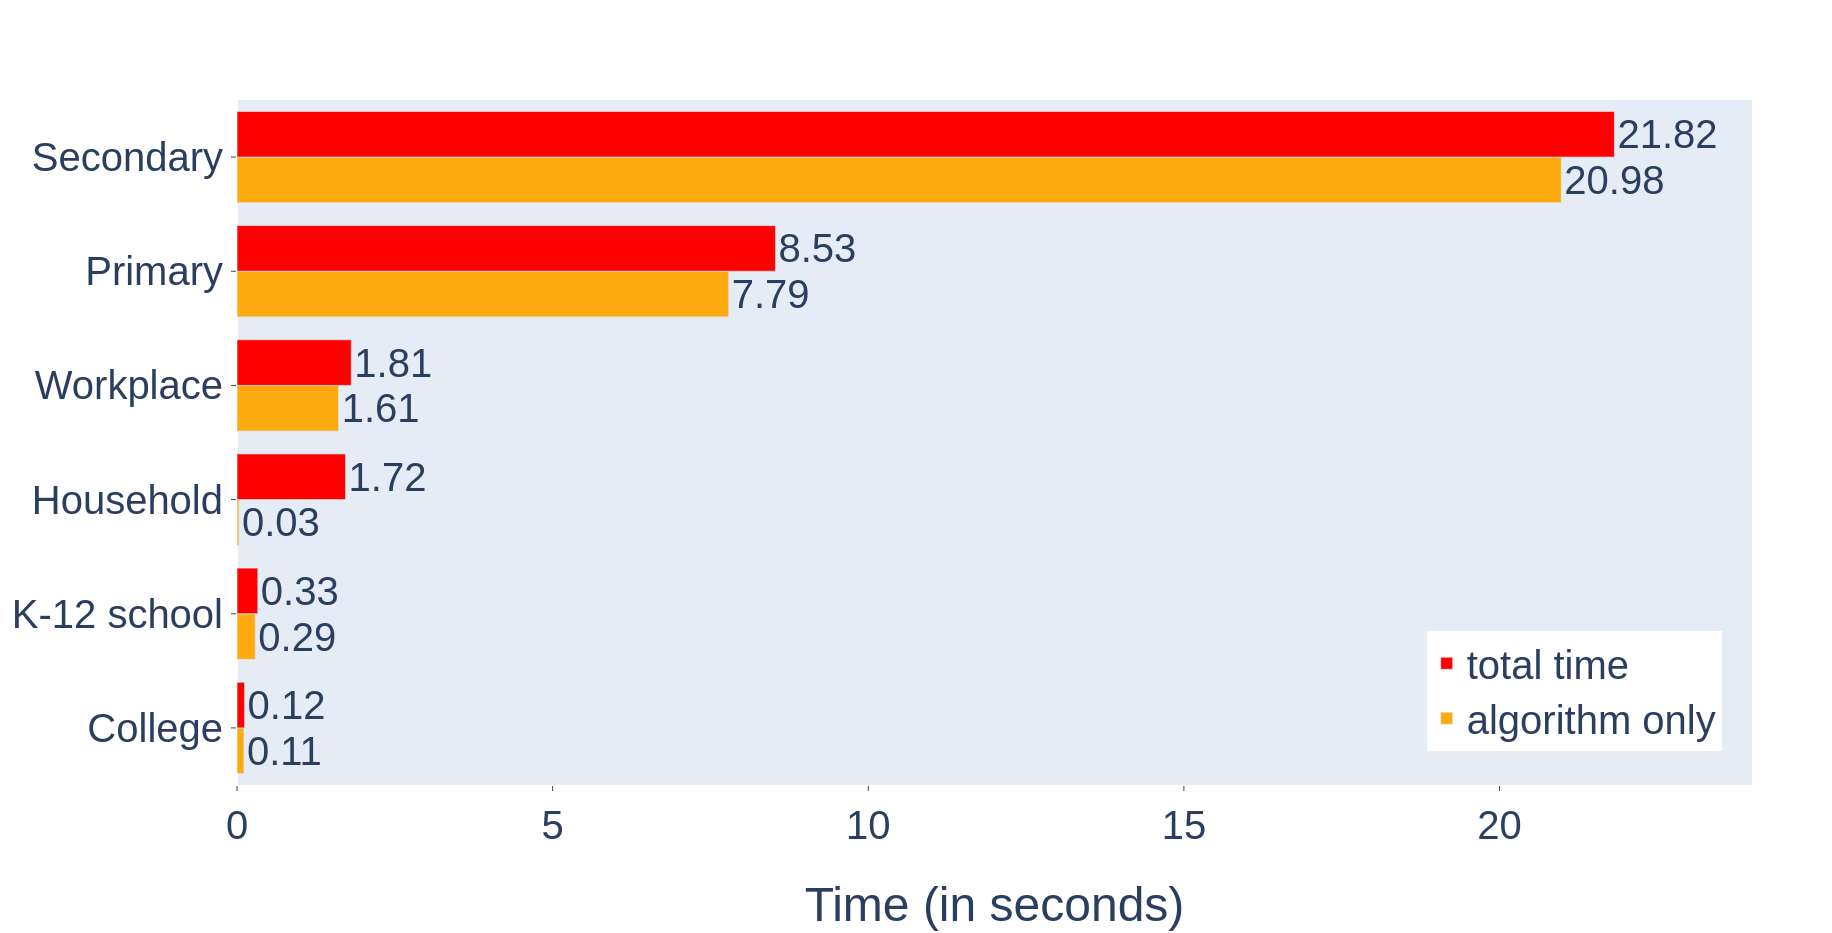
\includegraphics[width=\linewidth]{4 - Sampling/fig/standard/standard_times_type_totals.png}
    \caption{Total daily average infector runtime (in milliseconds) per pool type using \textsc{All-to-All}, based on a 7-day week. \textit{Total time} represents the time it takes to call infector on all of the pools and \textit{algorithm only} represents the total time spent in the infector for a pool type. Simulation run on 11M population for 7 days without holidays using 1 thread (configurations in Appendix \ref{appendix:configurations}).}
    \label{fig:standard_times_type_totals}
\end{figure}

\subsection{Reversed contact vector}
\label{subsec:reversed_contact_vector}
Stride has a built-in unit-testing feature designed to assist the programmers when developing. It tests the program on the basis of different parameters to see if the results, for example the number of infected people, are correct. Because there is randomness involved in a simulation, these results can differ every time. In order to determine whether the results are `correct', they need to lie within certain margins. This tool also verifies that the results are correct when using parallellization, which is necessary to catch multithreading issues such as race conditions \cite{race_condition}. This has proven useful during this thesis, but we will see in the upcoming sections that it does not always succeed in catching erroneous results. Therefore, we introduce another tool that will act as a benchmark in the upcoming sections, which is the reversed contact vector. From Section \ref{subsec:contact_matrix} we know that Stride uses the contact vectors to calculate the contact probabilities that are being used by the infector algorithms. The reversed contact vectors are the reconstructions of those original ones and are built up from the results of a simulation.
\\\\
Figure \ref{fig:reversed_cr_standard} shows the reversed contact vectors of Stride for every pool type and compares them with the original contact vectors. We can clearly see that they are not an exact match, but this is due to the adjustment factors that are taken into account when calculating the contact probabilities, as shown in Algorithm \ref{alg:contact_probability}. The original contact vectors start from the age of one, while Stride starts from age zero, which causes the reversed vectors to shift a little bit to the left. The K-12 school and college contact pools use the school contact vector for their contact probabilities and are therefore both compared to this vector.
\\\\
Figures \ref{fig:reversed_cr_standard_k12school}, \ref{fig:reversed_cr_standard_college} and \ref{fig:reversed_cr_standard_workplace} show that the reversed contact rate for some ages are zero. The reason for this is the way these reversed vectors are built. The results that our tool uses, are generated by an actual Stride simulation. They are saved in a file that contains all the logged events among which the contacts, transmissions, etc. These events are saved line by line and specify the IDs of both individuals in an event, their ages, the probability that the event would happen, and many more. If every single event in a simulation would be logged, the size of the log file would be several gigabytes per day for the 600K population. To determine how much needs to be logged, a parameter can be set for the number of people that need to be tracked. These people are then randomly chosen when initialising the simulator and only their events are logged. Our reversed contact rates also do not take into account that someone might not be a member of a certain pool type, such as an unemployed adult or an adult that works but who is not a teacher and thus has zero contacts at a school. This is the reason that the reversed rates for some ages are noticeably less than the original ones.
\\\\
In order to get the best results for these reversed contact vectors, we set the number of infected people in the beginning to zero. This leads to no infections during the entire simulation so individuals would not change their behaviour because they are infected. We set the number of people that will be logged to 50,000 and only simulate 28 days for these results, which is enough to get accurate results for every pool type. A side effect of this method is that some ages for which there are not that many individuals in a particular pool type, the results may show that the contact rate is zero. This is due to the random selection of people that need to be tracked, which causes some ages to not be represented in a pool type. An example of this are the professors of a college, ages 23 to 65, for which Figure \ref{fig:reversed_cr_standard_college} shows they do not have any contacts which is not true. The other possibility for this to happen is that there are no individuals in the population that meet the criteria for a certain age and pool type. All in all the reversed contact vectors still provide enough data to evaluate the model. In the upcoming sections we will ignore the original contact rates and only use the reversed vectors from Figure \ref{fig:reversed_cr_standard} as reference point.

\begin{figure}
    \centering
    \begin{subfigure}{.8\linewidth}
        \centering
        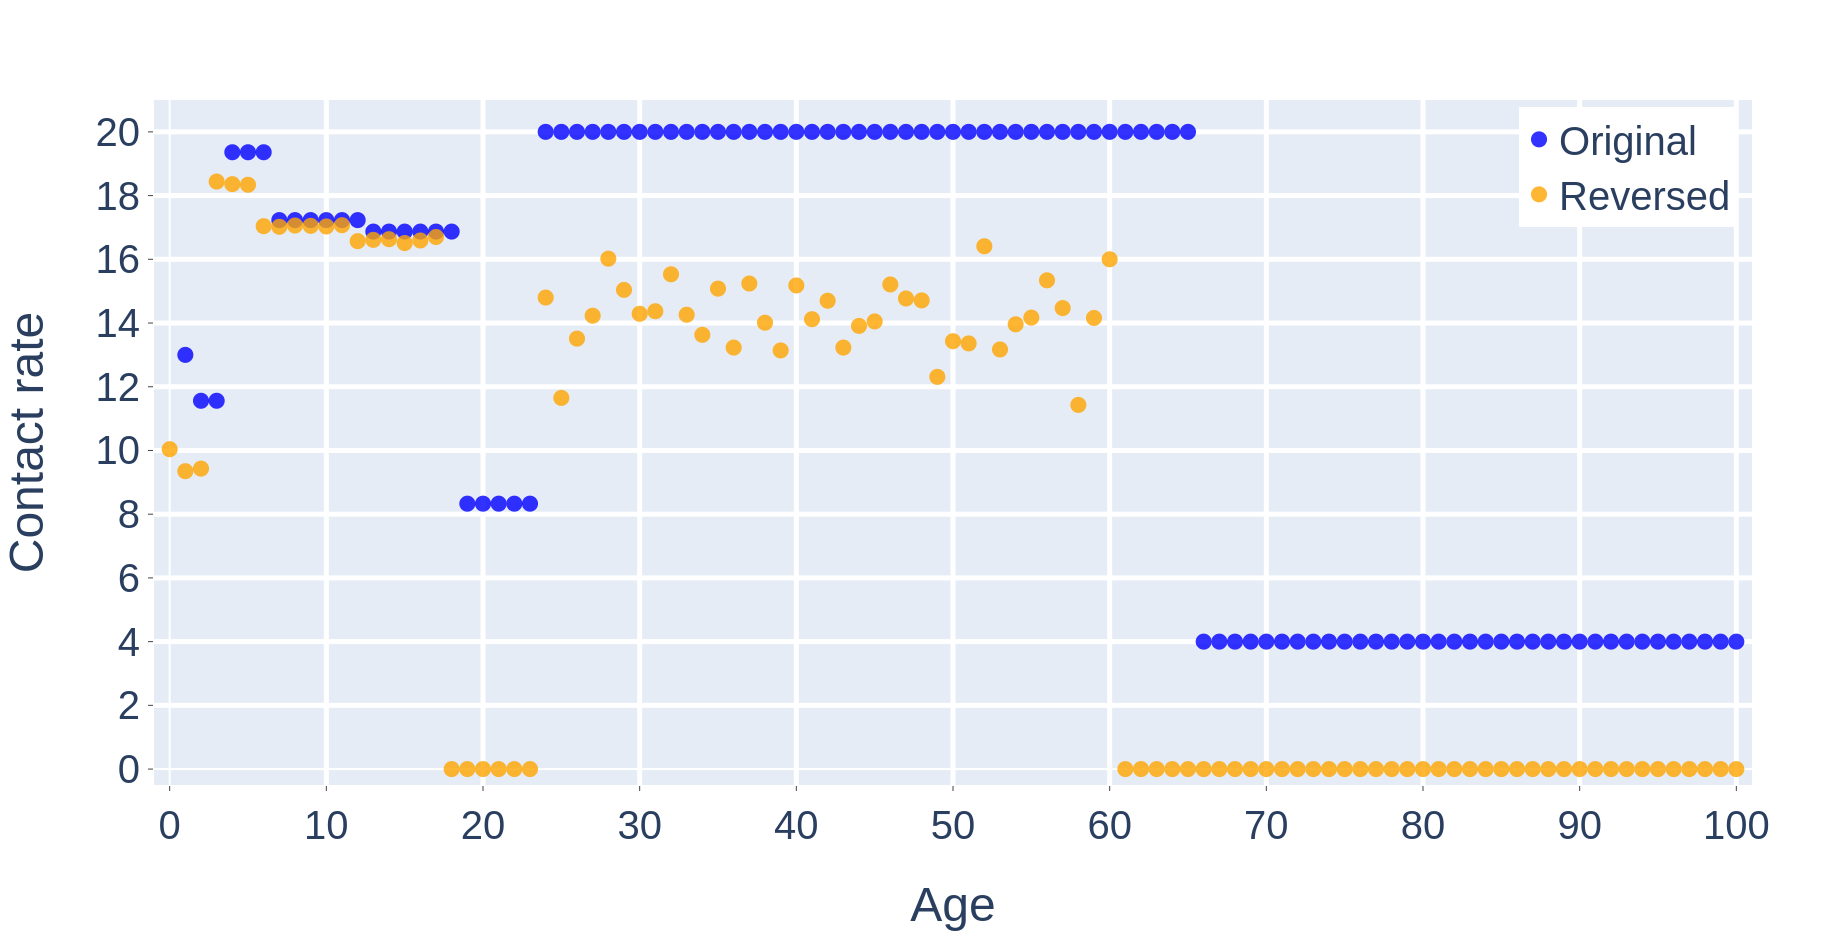
\includegraphics[width=\textwidth]{4 - Sampling/fig/standard/standard_reverse_cr_k12school.png}
        \caption{K-12 school}
        \label{fig:reversed_cr_standard_k12school}
    \end{subfigure}
    \begin{subfigure}{.8\linewidth}
        \centering
        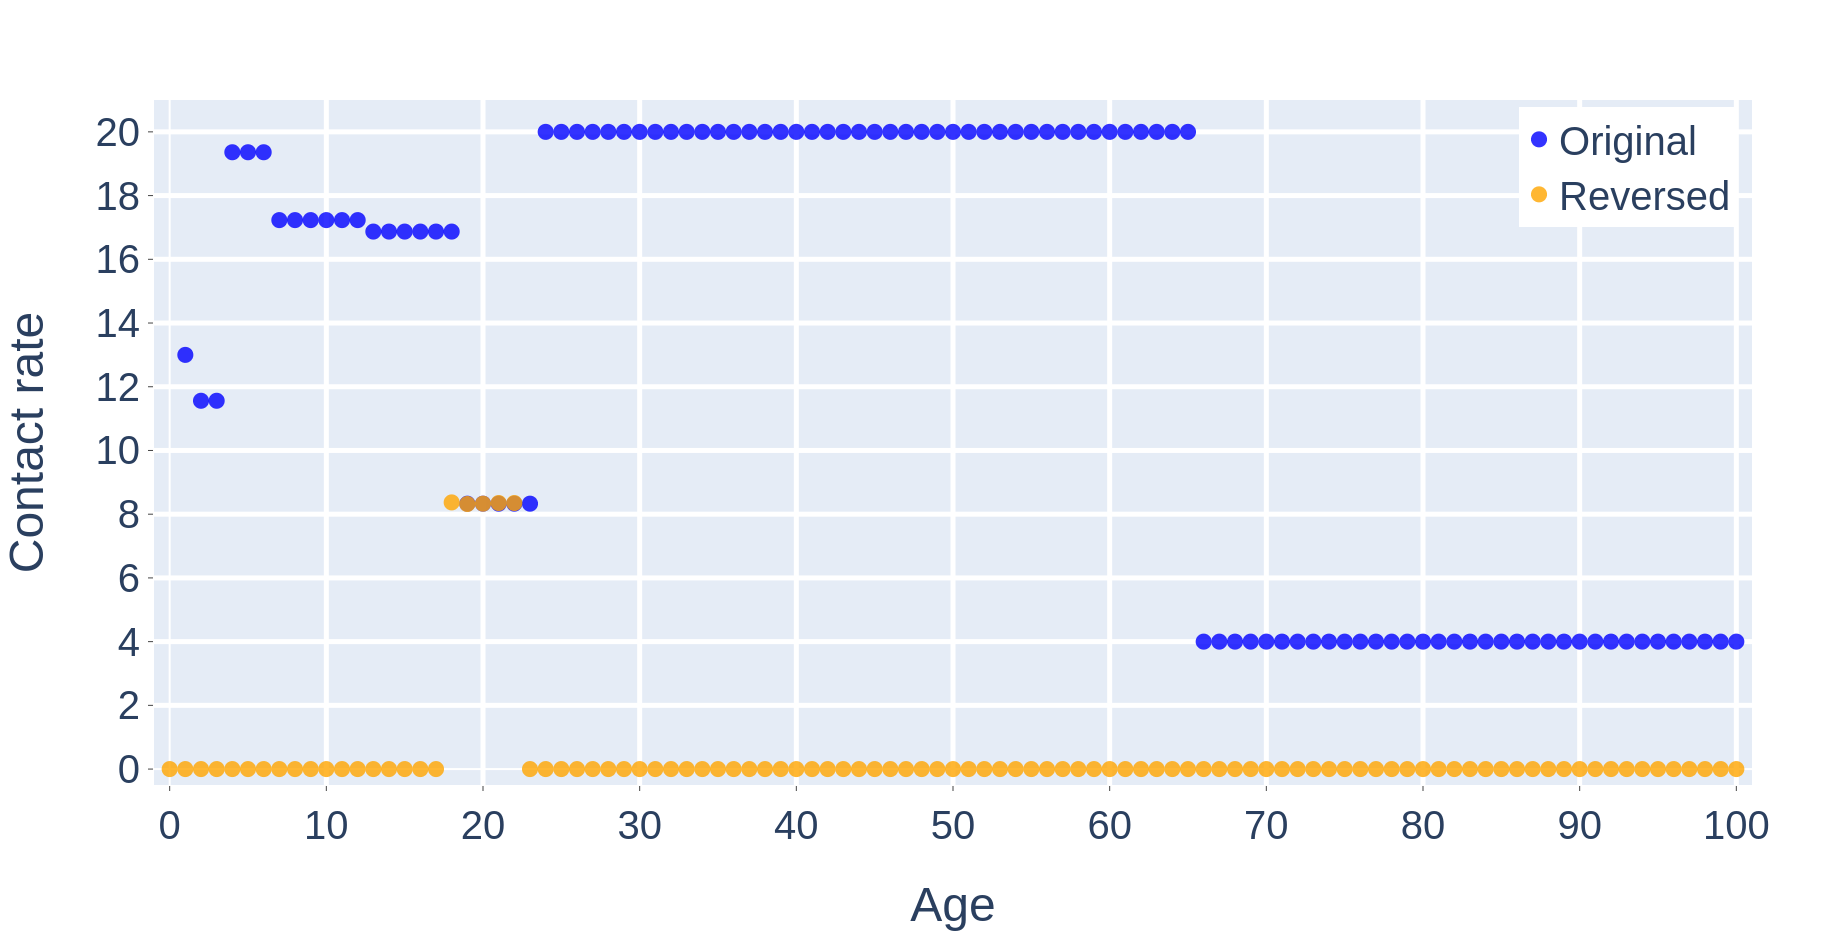
\includegraphics[width=\textwidth]{4 - Sampling/fig/standard/standard_reverse_cr_college.png}
        \caption{College}
        \label{fig:reversed_cr_standard_college}
    \end{subfigure}
    \begin{subfigure}{.8\linewidth}
        \centering
        \includegraphics[width=\textwidth]{4 - Sampling/fig/standard/standard_reverse_cr_workplace.png}
        \caption{Workplace}
        \label{fig:reversed_cr_standard_workplace}
    \end{subfigure}
    \caption{Comparison of the reversed contact rates with the original contact rates from Section \ref{subsec:contact_matrix}.}
\end{figure}
\begin{figure}\ContinuedFloat
    \centering
    \begin{subfigure}{.8\linewidth}
        \centering
        \includegraphics[width=\textwidth]{4 - Sampling/fig/standard/standard_reverse_cr_primary.png}
        \caption{Primary community}
        \label{fig:reversed_cr_standard_primary}
    \end{subfigure}
    \begin{subfigure}{.8\linewidth}
        \centering
        \includegraphics[width=\textwidth]{4 - Sampling/fig/standard/standard_reverse_cr_secondary.png}
        \caption{Secondary community}
        \label{fig:reversed_cr_standard_secondary}
    \end{subfigure}
    \caption{Comparison of the reversed contact rates with the original contact rates from Section \ref{subsec:contact_matrix}.}
    \label{fig:reversed_cr_standard}
\end{figure}

\section{Iterative intervals}
\label{sec:iterative_intervals}
Our general idea is to use a sampling approach to optimise the \textsc{All-to-All} infector algorithm. However, as we discussed, the main issue for this is the contact probability between two individuals, which is calculated based on the age of the two individuals. In order to use our approach, this issue first must be resolved. This section explains a solution for the contact probability calculations, which also happens to be a major improvement already.

\subsection{Age intervals}
\label{subsec:age_intervals}
Since our problem is about the calculation of the contact probabilities, this is where we should look for the solution. Algorithm \ref{alg:contact_probability} shows how this calculation uses the contact rates of two persons and takes the minimum of the two rates to determine the probability. If we want to take a sample from a pool with the binomial distribution we talked about, we would need a contact probability that applies to everyone in the pool. Unfortunately, this is not possible because the contact rates are different depending on age. However, if we look at the contact vectors in Section \ref{subsec:contact_matrix}, we notice that the contact rates are the same for a lot of ages. This means that the contact probability in one pool is the same in a lot of cases. Thus, we could use the same contact probability for different pairs of individuals and still get correct results. Following this logic, we split up the contact pools in groups, where everyone in a group has the same contact rate. Then, if our model were to calculate the contacts for a pool, it would only need to calculate one contact probability for every pair of groups. Although the infector would still have a quadratic time complexity since everyone still gets compared with everyone, it would reduce the runtime by reducing the number of contact probabilities that need to be calculated.
\\\\
We now need to determine for every pool type how the pool members will be divided in groups. For this we look at the contact vectors from Section \ref{subsec:contact_matrix} to decide the ages with the same contact rate. Because the ages with the same contact rate lie in age intervals for every pool type, we can simply use these age intervals to represent a `same contact rate group'. Table \ref{tab:age_intervals} shows the age intervals for every contact pool type with their corresponding contact rates. The first age intervals for the primary and secondary community have two contact rates, because age one has a different rate (the upper one) than ages two and three. Since these rates are almost the same, we choose to not split them up. However, for the school contact type we have a separate interval for age one, because its rate is much more different. Another reason for splitting these up or not, is the way these ages are distributed in the pools. In a school contact pool, almost everyone except the teacher has the same age, while a community pool can contain all the possible ages. This results in less intervals for the community pools, which will be beneficial for our sampling approach in the next sections. When we now determine the contact probability between two intervals, we use the age of the first member of an interval. Intervals that contain ages with multiple contact rates will thus be represented by the contact rate of the first member, which can be different depending on the pool since people in a pool do not have a predetermined order.

\begin{table}
    \centering
    \begin{subtable}[b]{0.45\textwidth}
        \centering
        \begin{tabular}{@{}ccr@{}}
            \toprule
            \# & Age interval & Rate \\ \midrule
            1 & {[} 1 {]} & 13.00 \\
            2 & {[} 2, 3 {]} & 11.56 \\
            3 & {[} 4, 6 {]} & 19.36 \\
            4 & {[} 7, 12 {]} & 17.23 \\
            5 & {[} 13, 18 {]} & 16.87 \\
            6 & {[} 19, 23 {]} & 8.33 \\
            7 & {[} 24, 65 {]} & 20.00 \\
            8 & {[} 66, $\infty$ {[} & 4 \\ \bottomrule
        \end{tabular}
        \caption{School (K-12 school and college).}
        \label{tab:age_intervals_school}
    \end{subtable}
    \hfill
    \begin{subtable}[b]{0.45\textwidth}
        \centering
        \begin{tabular}{ccr}
            \hline
            \# & \multicolumn{1}{l}{Age interval} & \multicolumn{1}{l}{Rate} \\ \hline
            1 & {[} 0, 18 {]} & 0 \\
            2 & {[} 19, 65 {]} & 7.57 \\
            3 & {[} 66, $\infty$ {[} & 5.00 \\ \hline
        \end{tabular}
        \caption{Workplace}
        \label{tab:age_intervals_workplace}
    \end{subtable}
    \newline
    \newline
    \begin{subtable}[h]{0.45\textwidth}
        \centering
        \begin{tabular}{ccr}
            \hline
            \# & \multicolumn{1}{l}{Age interval} & Rate \\ \hline
            1 & {[} 0, 3 {]} & \begin{tabular}[c]{@{}r@{}}3.62\\ 3.80\end{tabular} \\
            2 & {[} 4, 6 {]} & 5.92 \\
            3 & {[} 7, 12 {]} & 12.04 \\
            4 & {[} 13, 18 {]} & 9.60 \\
            5 & {[} 19, 23 {]} & 15.92 \\
            6 & {[} 24, 45 {]} & 14.50 \\
            7 & {[} 46, 65 {]} & 12.05 \\
            8 & {[} 66, 75 {]} & 9.62 \\
            9 & {[} 75, $\infty$ {[} & 6.06 \\ \hline
        \end{tabular}
        \caption{Primary community.}
        \label{tab:age_intervals_primary}
    \end{subtable}
    \hfill
    \begin{subtable}[h]{0.45\textwidth}
        \centering
        \begin{tabular}{ccr}
            \hline
            \# & \multicolumn{1}{l}{Age interval} & Rate \\ \hline
            1 & {[} 0, 3 {]} & \begin{tabular}[c]{@{}r@{}}3.01\\ 3.47\end{tabular} \\
            2 & {[} 4, 6 {]} & 3.05 \\
            3 & {[} 7, 12 {]} & 5.75 \\
            4 & {[} 13, 18 {]} & 14.33 \\
            5 & {[} 19, 23 {]} & 11.42 \\
            6 & {[} 24, 45 {]} & 15.73 \\
            7 & {[} 46, 65 {]} & 14.01 \\
            8 & {[} 66, 75 {]} & 8.60 \\
            9 & {[} 75, $\infty$ {[} & 5.04 \\ \hline
        \end{tabular}
        \caption{Secondary community.}
        \label{tab:age_intervals_secondary}
    \end{subtable}
    \caption{Age intervals for the different contact pool types with their corresponding contact rates. The intervals with multiple contact rates are represented by the rate of the first member, which is random and thus different per pool.}
    \label{tab:age_intervals}
\end{table}

\subsection{Implementation}
\label{subsec:implementation_iterative_intervals}
Now we can use the age intervals to implement our improved algorithm. Algorithm \ref{alg:age_sorting} presents the pseudo code for the sorting of pool members in these different intervals, which also returns the number of members in every interval. This sorting function will also be used for the upcoming approaches in the next sections. The implementation of our approach that uses the age intervals is presented in Algorithm \ref{alg:iterative_intervals}. The household pools still use the original \textsc{All-to-All} algorithm, since they contain maximum six persons. The rest of the pools use our intervals approach, where every intervals gets compared with every other interval including itself. For every pair of intervals, only one contact probability is calculated. Then, the algorithm iterates over both intervals and uses the contact probability for every pair of members from two intervals to see if they have contact and transmit the disease. Because this algorithm still compares everyone with everyone in a pool by iterating over the intervals and their members, we will refer to this \textsc{All-to-All} infector approach as \textsc{Iterative-intervals} from now on.

\begin{algorithm}
\caption{Pseudo code of the function that sorts the members in age intervals.}
\label{alg:age_sorting}
\begin{algorithmic}[1]
    \Require{$P_{1} \dots P_{N}$, $type$} \Comment{All members of the pool and type of pool}\;
    \Ensure{$P[\;] sorted$, $S[\;]$} \Comment{Sorted members and interval sizes}
    \Statex
    \State $intervals[\;] \gets$ \Call{age\_intervals}{$type$}\Comment{Maximum ages per interval (ascending)}
    \State $N_{intervals} \gets$ \Call{sizeof}{$intervals[\;]$} \Comment{Number of intervals}
    \State $i_{unsorted} \gets 1$\Comment{Index of first unsorted member}
    \State $S[\;] \gets [N_{intervals}]$\Comment{Interval sizes, zero at start}
    \Statex
    \For{$i_{interval} \gets 1$ to ($N_{intervals}-1)$}\Comment{Iterate over the intervals}
        \State $age_{interval} \gets intervals[i_{interval}]$ \Comment{Maximum age of the interval}
        \For{$i_{member} \gets i_{unsorted}$ to $N$}\Comment{Iterate over the unsorted members}
            \State $age_{member} \gets$ \Call{age}{$P[i_{member}]$}
            \If{$age_{member} \leq age_{interval}$}
                \If{$i_{member} > i_{unsorted}$}
                    \State \Call{swap}{$P[i_{unsorted}], P[i_{member}]$}
                \EndIf
                \State $i_{unsorted}++$
                \State $S[i_{interval}]++$
            \EndIf
        \EndFor
    \EndFor
    \State $S[N_{intervals}] \gets N - i_{unsorted} + 1$ \Comment{Remaining unsorted members}
    \Statex
    \State \Return $S[\;]$
\end{algorithmic}
\end{algorithm}

\begin{algorithm}
\caption{Pseudo code of the \textsc{Iterative-intervals} infector.}
\label{alg:iterative_intervals}
\begin{algorithmic}[1]
    \Require{$P_{1} \dots P_{N}$, $type$} \Comment{All members of the pool and type of pool}\;
    \Statex
    \If{$type = household$}
        \State original \textsc{All-to-All} \Comment{Algorithm \ref{alg:all-to-all}}
    \Else
        \State $S[\;] \gets$ \Call{sort\_intervals}{$P[\;], type$}\Comment{Algorithm \ref{alg:age_sorting}}
        \State $N_{intervals} \gets$ \Call{sizeof}{$S[\;]$} \Comment{Number of intervals}
        \Statex
        \For{$interval_{1} \gets 1$ to $N_{intervals}$} \Comment{Iterate intervals}
            \For{$interval_{2} \gets interval_{1}$ to $N_{intervals}$} \Comment{Iterate remaining intervals}
                \State $C_{prob} \gets$ \Call{ContactProbability}{$P[interval_{1}], P[interval_{2}]$}\Comment{Algorithm \ref{alg:contact_probability}}
                \Statex
                \If{$interval_{1}$ = $interval_{2}$}
                    \For{$i \gets 1$ to $S[interval_{1}]$}
                        \State $P_{1} \gets$ member $i$ of $interval_{1}$
                        \If{$P_{1}$ not in pool}
                            \State continue to next $P_{1}$
                        \EndIf
                        \For{$j \gets i$ to $S[interval_{1}]$}
                            \State $P_{2} \gets$ member $j$ of $interval_{1}$
                            \If{$P_{1} = P_{2}$ OR $P_{2}$ not in pool}
                                \State Continue to next $j$
                            \EndIf
                            \If{\Call{BernoulliTrial}{$C_{prob}$}}
                                \State register contact
                                \If{$P_{1}$ or $P_{2}$ susceptible and other infectious}
                                    \State $T_{prob} \gets$ transmission probability
                                    \If{\Call{BernoulliTrial}{$T_{prob}$}}
                                        \State infect the susceptible one
                                    \EndIf
                                \EndIf
                            \EndIf
                        \EndFor
                    \EndFor
                \Else
                    \Foreach{member $P_{1}$ in $interval_{1}$}
                        \If{$P_{1}$ not in pool}
                            \State continue to next $P_{1}$
                        \EndIf
                        \Foreach{member $P_{2}$ in $interval_{2}$}
                            \If{$P_{2}$ not in pool OR $P_{1} = P_{2}$}
                                \State continue to next $P_{2}$
                            \EndIf
                            \If{\Call{BernoulliTrial}{$C_{prob}$}}
                                \State register contact
                                \If{$P_{1}$ or $P_{2}$ susceptible and other infectious}
                                    \State $T_{prob} \gets$ transmission probability
                                    \If{\Call{BernoulliTrial}{$T_{prob}$}}
                                        \State infect the susceptible one
                                    \EndIf
                                \EndIf
                            \EndIf
                        \EndForeach
                    \EndForeach
                \EndIf
            \EndFor
        \EndFor
    \EndIf
\end{algorithmic}
\end{algorithm}

\subsection{Correctness}
\label{subsec:correctness_iterative_intervals}
We need to evaluate our approach and see if our model logic has not changed. For this we use the techniques discussed in Section \ref{subsec:reversed_contact_vector}, which are the built-in testing tool and the reversed contact vector. The testing tool only tells us if the range of the results are valid, which is the case. We then continue to compute the reversed contact rates, for which the results are displayed in Figure \ref{fig:ii_vs_standard_reverse_cr}. They show that the \textsc{Iterative-intervals} approach has almost identical reversed contact rates as the original \textsc{All-to-All} algorithm. Therefore, we conclude that \textsc{Iterative-intervals} is a valid \textsc{All-to-All} algorithm.

\begin{figure}
    \centering
    \begin{subfigure}{.8\linewidth}
        \centering
        \includegraphics[width=\textwidth]{4 - Sampling/fig/iterative_intervals/ii_vs_standard_reverse_cr_k12school.png}
        \caption{K-12 school}
        \label{fig:ii_vs_standard_reversed_cr_standard_k12school}
    \end{subfigure}
    \begin{subfigure}{.8\linewidth}
        \centering
        \includegraphics[width=\textwidth]{4 - Sampling/fig/iterative_intervals/ii_vs_standard_reverse_cr_college.png}
        \caption{College}
        \label{fig:ii_vs_standard_reversed_cr_standard_college}
    \end{subfigure}
    \begin{subfigure}{.8\linewidth}
        \centering
        \includegraphics[width=\textwidth]{4 - Sampling/fig/iterative_intervals/ii_vs_standard_reverse_cr_workplace.png}
        \caption{Workplace}
        \label{fig:ii_vs_standard_reversed_cr_standard_workplace}
    \end{subfigure}
    \caption{Comparison of the \textsc{Iterative-intervals} reversed contact rates with the original \textsc{All-to-All} reversed contact rates.}
\end{figure}
\begin{figure}\ContinuedFloat
    \centering
    \begin{subfigure}{.8\linewidth}
        \centering
        \includegraphics[width=\textwidth]{4 - Sampling/fig/iterative_intervals/ii_vs_standard_reverse_cr_primary.png}
        \caption{Primary community}
        \label{fig:ii_vs_standard_reversed_cr_standard_primary}
    \end{subfigure}
    \begin{subfigure}{.8\linewidth}
        \centering
        \includegraphics[width=\textwidth]{4 - Sampling/fig/iterative_intervals/ii_vs_standard_reverse_cr_secondary.png}
        \caption{Secondary community}
        \label{fig:ii_vs_standard_reversed_cr_standard_secondary}
    \end{subfigure}
    \caption{Comparison of the \textsc{Iterative-intervals} reversed contact rates with the original \textsc{All-to-All} reversed contact rates from Section \ref{subsec:reversed_contact_vector}.}
    \label{fig:ii_vs_standard_reverse_cr}
\end{figure}

\subsection{Performance}
\label{subsec:performance_iterative_intervals}
At last, we need to examine the \textsc{Iterative-intervals} approach to see if it is indeed an optimisation. The first performance test that we will discuss is the runtime of the infector, which is the vast majority of the total runtime in an \textsc{All-to-All} simulation. Figure \ref{fig:ii_vs_standard_infector} shows the infector runtimes of the \textsc{Iterative-intervals} approach compared to the original algorithm, which clearly indicates that our new approach is a big improvement. Table \ref{tab:ii_vs_standard_runtimes} confirms that we achieve an average speedup of 1.86 on the infector and 1.81 on the total simulation runtime.
\\\\
Next to the total runtime, we are also interested in how our optimisation affects the infector runtime regarding the pool type and size. In Section \ref{subsec:infector_runtimes} we showed how the average infector runtime has a quadratic curve in function of the pool size. Because the infector algorithm now works differently depending on the pool type, we need to examine the runtimes separately for every pool type. Figure \ref{fig:times_avg_ii} shows these average infector runtime results of the \textsc{Iterative-intervals} approach compared to the original algorithm. Here we can see that our new approach still has a quadratic curve, but that it becomes increasingly faster than the original the larger the pool. The differences for the K-12 school and college pool types are very little and will be discussed more in Section \ref{subsec:performance_sampling_with_iteration}.
\\\\
In Section \ref{subsec:infector_runtimes} we discussed the runtime of every pool type based on a 7-day week, which was also shown in Figure \ref{fig:standard_times_type_totals}. This taught us which pool types have a larger impact on the general runtime than others. Now we are only interested in how our approach affects the actual runtime of every pool type. Figure \ref{fig:ii_vs_standard_type_totals} shows the total runtimes for every pool type on an active day using different approaches, where we can see the impact of our approach on every pool type. The optimisations are most beneficial to the community pools and the workplace, while the household now takes more time to compute. This is due to the extra if-test in Algorithm \ref{alg:iterative_intervals} and is detrimental to its runtime. Altogether, the \textsc{Iterative-intervals} approach is a major optimisation for the \textsc{All-to-All} infector by only eliminating the amount of contact probability calculations.

\begin{figure}
    \centering
    \includegraphics[width=\textwidth]{4 - Sampling/fig/iterative_intervals/ii_vs_standard_infector.png}
    \caption{Comparison of the infector runtimes between the original and \textsc{Iterative-intervals} approaches. Simulations run on 11M population for 100 days without holidays using 1 thread (configurations in Appendix \ref{appendix:configurations}).}
    \label{fig:ii_vs_standard_infector}
\end{figure}

\begin{table}
    \centering
    \begin{tabular}{@{}lrr@{}}
        \toprule
        \textsc{All-to-All} & Infector & Total \\ \midrule
        original & 32.63 & 33.77 \\
        iterative-intervals & 17.54 & 18.67 \\ \hdashline[1pt/1pt]
        speedup & 1.86 & 1.81 \\ \bottomrule
    \end{tabular}
    \caption{Comparison of the average daily runtimes between the original and \textsc{Iterative-intervals} approach. Simulations run on 11M population for 100 days without holidays using 1 thread (configurations in Appendix \ref{appendix:configurations}).}
    \label{tab:ii_vs_standard_runtimes}
\end{table}

\begin{figure}
    \centering
    \begin{subfigure}{.78\linewidth}
        \centering
        \includegraphics[width=\textwidth]{4 - Sampling/fig/iterative_intervals/times_avg_ii_workplace.png}
        \caption{Workplace}
        \label{fig:times_avg_ii_workplace}
    \end{subfigure}
    \begin{subfigure}{.78\linewidth}
        \centering
        \includegraphics[width=\textwidth]{4 - Sampling/fig/iterative_intervals/times_avg_ii_primary.png}
        \caption{Primary community}
        \label{fig:times_avg_ii_primary}
    \end{subfigure}
    \begin{subfigure}{.78\linewidth}
        \centering
        \includegraphics[width=\textwidth]{4 - Sampling/fig/iterative_intervals/times_avg_ii_secondary.png}
        \caption{Secondary community}
        \label{fig:times_avg_ii_secondary}
    \end{subfigure}
    \caption{Average infector runtimes (in milliseconds) per pool size using the original \textsc{All-to-All} and \textsc{Iterative-intervals}. Simulations run on 11M population for 100 days without holidays using 1 thread (configurations in Appendix \ref{appendix:configurations}).}
    \label{fig:times_avg_ii}
\end{figure}

\begin{figure}
    \centering
    \includegraphics[width=\linewidth]{4 - Sampling/fig/iterative_intervals/ii_vs_standard_type_totals.png}
    \caption{Comparison of the total infector runtimes (in seconds) per pool type on a day in which its pools are active. Simulations run on 11M population for 100 days without holidays using 1 thread (configurations in Appendix \ref{appendix:configurations}).}
    \label{fig:ii_vs_standard_type_totals}
\end{figure}

\section{Sampling with iteration}
\label{sec:sampling_with_iteration}
Recall that the issue of our general sampling idea was the contact probability. For every member in a pool we want to calculate a sample size with a binomial distribution that needs to know the pool size and the probability. What we have learned from \textsc{Iterative-intervals} can now be used to implement the sampling idea. We again divide our pool in these intervals after which the intervals get compared in pairs. Then, we can calculate the sample size, which is the number of contacts that someone will have with the members in another interval. However, this raises a question about the contact calculations for members in the same interval. Calculating if two members have contact with each other happens only once, which is also the case for calculating contacts between two intervals. Every pair of intervals is only considered once to calculate the contacts between their members. If we now want to use the sampling approach for the members inside an interval, taking a sample for every member would cause the algorithm to consider two individuals twice. To avoid this problem, we will not use the sampling approach when comparing members in the same interval, but instead use the \textsc{Iterative-intervals} approach. Calculating contact for people in the same interval will thus calculate one contact probability and then compare everyone with everyone. Since our new approach uses sampling combined with the \textsc{Iterative-intervals}, we refer to it from now on as the \textsc{Sampling-with-iteration} approach.

\subsection{Implementation}
\label{subsec:implementation_sampling_with_iteration}
The pseudo code of the \textsc{Sampling-with-iteration} approach is given in Algorithm \ref{alg:sampling_with_iteration}. Just like the \textsc{Iterative-intervals}, the household type pools still use the original \textsc{All-to-All} method because their maximum size is six individuals, while the rest of the pools start off with dividing their members in the age intervals. Then, all of the intervals get compared once with each other. Like we said, the contacts between the people in the same interval are calculated in the \textsc{Iterative-intervals} way, where a double for-loop compares everyone with each other and only one contact probability is calculated for all of them. The comparisons with the other intervals work by iterating over the members of one interval, where for every person $P_{1}$ a sample size gets calculated by the binomial distribution based on the number of people in the other interval, $interval_{2}$, and the contact probability between the members of the two intervals. This sample size indicates the number of people from $interval_{2}$ that $P_{1}$ will have contact with. If the sample size is zero we can just skip $P_{1}$ and continue to the next one, because there are no contacts for the current $P_{1}$ with members in $interval_{2}$. If the sample size is equal to the number of people in $interval_{2}$, it means that $P_{1}$ will have contact with everyone in the interval. When this happens, we do not need to sample and can just iterate over the entire interval and handle the contacts and transmissions between $P_{1}$ and everyone in $interval_{2}$. If the sample size is smaller than the size of $interval_{2}$, we need to determine who will have contact with $P_{1}$. To select these contacts, we `draw' a person from $interval_{2}$ based on a random number. If this randomly selected individual is present in the pool and if we have not already drawn him for the same $P_{1}$, we register their contact and calculate the transmission as we know.

\begin{algorithm}
\caption{Pseudo code of the \textsc{Sampling-with-iteration} infector.}
\label{alg:sampling_with_iteration}
\begin{algorithmic}[1]
    \Require{$P_{1} \dots P_{N}$, $type$} \Comment{All members of the pool and type of pool}\;
    \Statex
    \If{$type = household$}
        \State original \textsc{All-to-All} \Comment{Algorithm \ref{alg:all-to-all}}
    \Else
        \State $S[\;] \gets$ \Call{sort\_intervals}{$P[\;], type$}\Comment{Algorithm \ref{alg:age_sorting}, returns interval sizes}
        \State $N_{intervals} \gets$ \Call{sizeof}{$S[\;]$} \Comment{Number of intervals}
        \Statex
        \For{$interval_{1} \gets 1$ to $N_{intervals}$} \Comment{Iterate intervals}
            \For{$interval_{2} \gets interval_{1}$ to $N_{intervals}$} \Comment{Iterate remaining intervals}
                \State $C_{prob} \gets$ \Call{contact\_probability}{$interval_{1}, interval_{2}$} \Comment{Algorithm \ref{alg:contact_probability}}
                \Statex
                \If{$interval_{1} = interval_{2}$}
                    \State \textsc{Iterative-intervals} \Comment{Algorithm \ref{alg:iterative_intervals}}
                \Else
                    \Foreach{member $P_{1}$ in $interval_{1}$}
                        \If{$P_{1}$ not in pool}
                            \State continue to next $P_{1}$
                        \EndIf
                        \State $sample \gets$ \Call{binomial}{$S[interval_{2}], C_{prob}$} \Comment{Binomial distribution}
                        \If{$sample$ = 0}
                            \State continue to next $P_{1}$
                        \ElsIf{$sample$ = $S[interval_{2}]$}
                            \State iterate over $interval_{2}$ and register contact with everyone
                        \Else
                            \State $draws_{all} \gets 0$ \Comment{Number of draws}
                            \State $draws_{good} \gets 0$ \Comment{Number of good draws}
                            \State $drawn\_members \gets [\;]$
                            \Statex
                            \While{$draws_{good} < sample$ AND $draws_{all} < S[interval_{2}]$}
                                \State $P_{2} \gets$ random member of $interval_{2}$
                                \If{$P_{2}$ in $drawn\_members$}
                                    \State draw next $P_{2}$
                                \EndIf
                                \State add $P_{2}$ to $drawn\_members[\;]$
                                \State $++draws_{all}$
                                \If{$P_{2}$ not in pool}
                                    \State draw next $P_{2}$
                                \EndIf
                                \State $++draws_{good}$
                                \State register contact
                                \If{$P_{1}$ or $P_{2}$ susceptible and other infectious}
                                    \State $T_{prob} \gets$ transmission probability
                                    \If{\Call{BernoulliTrial}{$T_{prob}$}}
                                        \State infect the susceptible one
                                    \EndIf
                                \EndIf
                            \EndWhile
                        \EndIf
                    \EndForeach
                \EndIf
            \EndFor
        \EndFor
    \EndIf
\end{algorithmic}
\end{algorithm}

\subsection{Correctness}
\label{subsec:correctness_sampling_with_iteration}
Again we need to make sure that this approach is also correct. The first step is to run the built-in testing tool to see if the results, such as the number of infected people, lie within a certain interval and that it can also be used with parallellization. The \textsc{Sampling-with-iteration} algorithm passed this test, so we then continue to compute the reversed contact vectors, which are displayed in Figure \ref{fig:swi_vs_standard_reversed_cr}. The reversed rates of the original \textsc{All-to-All} algorithm are very similar to the reversed rates of the \textsc{Sampling-with-iteration} approach. Because this new approach passed both tests, we conclude that it is a valid \textsc{All-to-All} algorithm.

\begin{figure}
    \centering
    \begin{subfigure}{.8\linewidth}
        \centering
        \includegraphics[width=\textwidth]{4 - Sampling/fig/sampling_with_iteration/swi_vs_standard_reverse_cr_k12school.png}
        \caption{K-12 school}
        \label{fig:swi_vs_standard_reversed_cr_k12school}
    \end{subfigure}
    \begin{subfigure}{.8\linewidth}
        \centering
        \includegraphics[width=\textwidth]{4 - Sampling/fig/sampling_with_iteration/swi_vs_standard_reverse_cr_college.png}
        \caption{College}
        \label{fig:swi_vs_standard_reversed_cr_college}
    \end{subfigure}
    \begin{subfigure}{.8\linewidth}
        \centering
        \includegraphics[width=\textwidth]{4 - Sampling/fig/sampling_with_iteration/swi_vs_standard_reverse_cr_workplace.png}
        \caption{Workplace}
        \label{fig:swi_vs_standard_reversed_cr_workplace}
    \end{subfigure}
    \caption{Comparison of the \textsc{Sampling-with-iteration} reversed contact rates with the original \textsc{All-to-All} reversed contact rates from Section \ref{subsec:reversed_contact_vector}.}
\end{figure}
\begin{figure}\ContinuedFloat
    \centering
    \begin{subfigure}{.8\linewidth}
        \centering
        \includegraphics[width=\textwidth]{4 - Sampling/fig/sampling_with_iteration/swi_vs_standard_reverse_cr_primary.png}
        \caption{Primary community}
        \label{fig:swi_vs_standard_reversed_cr_primary}
    \end{subfigure}
    \begin{subfigure}{.8\linewidth}
        \centering
        \includegraphics[width=\textwidth]{4 - Sampling/fig/sampling_with_iteration/swi_vs_standard_reverse_cr_secondary.png}
        \caption{Secondary community}
        \label{fig:swi_vs_standard_reversed_cr_secondary}
    \end{subfigure}
    \caption{Comparison of the \textsc{Sampling-with-iteration} reversed contact rates with the original \textsc{All-to-All} reversed contact rates from Section \ref{subsec:reversed_contact_vector}.}
    \label{fig:swi_vs_standard_reversed_cr}
\end{figure}

\subsection{Performance}
\label{subsec:performance_sampling_with_iteration}
Now that we have verified the correctness of \textsc{Sampling-with-iteration}, we want to know how it performs compared to our other two approaches. Figure \ref{fig:swi_vs_rest_infector} shows the total infector runtime per day for the different algorithms, which proves that \textsc{Sampling-with-iteration} is even faster than \textsc{Iterative-intervals}. Table \ref{tab:swi_vs_standard_runtimes} reveals that our latest algorithm achieves an average total speedup of 2.33, which is due to the 2.47 average speedup in the infector.
\\\\
Our general idea from Section \ref{sec:general_idea} explains that the improvements we want to make will have the most impact on the larger pools because of the linear time complexity. Hence, Figure \ref{fig:times_avg_swi_pType_full} shows the average infector runtime regarding the pool size for the workplace and community pools. The community pools show that our \textsc{Sampling-with-iteration} approach has a somewhat linear curve, as we would expect, and that it is therefore a massive optimisation the larger the pool size. However, Figure \ref{fig:times_avg_swi_pType_workplace_full} shows that the workplace pools have a quadratic curve, similar to the \textsc{Iterative-intervals} algorithm. This is because the workplace has only three different age intervals where the [0,18]-interval is empty on most occasions. Secondly, almost everyone resides in the [19,65]-interval according to the workplace age distribution in Figure \ref{fig:workplace_age_distribution}. This causes workplace pools to spend most of their time calculating contacts between people in the same interval, which uses the \textsc{Iterative-intervals} method. \textsc{Sampling-with-iteration} has thus barely any effect on the workplace contact calculations. The community pools have nine different intervals that are all evenly distributed, which supports this explanation.
\\\\
The impact of our optimisation for every pool type is presented in Figure \ref{fig:swi_vs_rest_type_totals}, which shows that the community pools are the only ones that benefit from our new algorithm. The rest of the pools are all slower than the \textsc{Iterative-intervals} or even the original \textsc{All-to-All} approach. To further investigate this, a more detailed view on these pools is needed. Figure \ref{fig:times_avg_swi_pType} displays the average infector runtimes only for the pools that contain 300 people or less. The primary community in Figure \ref{fig:times_avg_swi_pType_primary}, as well as the secondary community in Figure \ref{fig:times_avg_swi_pType_secondary}, both show that the \textsc{Sampling-with-iteration} has the worst results for smaller pools. The reason for this is that the algorithm has extra overhead because of the binomial distribution calculation and the random member draws. When the intervals contain only a few individuals, the overhead takes more time than simply comparing everyone with everyone like the \textsc{Iterative-intervals} method does. Only pools with around 275 people achieve the fastest time with the \textsc{Sampling-with-iteration} approach, but it is already faster than the original one for pools with a size of at least 150 individuals. Figures \ref{fig:times_avg_swi_pType_k12school} and \ref{fig:times_avg_swi_pType_college} also show that the K-12 school and college pools lose speed using \textsc{Sampling-with-iteration}, for which the reason is also the predominant overhead in smaller pools and intervals.
\\\\
In the end we can conclude that our \textsc{Sampling-with-iteration} algorithm is a major optimisation compared to the original and \textsc{Iterative-intervals} \textsc{All-to-All} algorithms for larger pools. The time complexity of this algorithm is hard to define, because it is not completely linear due to the contact calculations between people in the same interval which still has a quadratic time complexity. Also, a double for-loop is used to iterate over the intervals which also results a quadratic time complexity in function of the number of intervals. However, this is negligible if there are not that many intervals as is the case for our different pool types. Altogether, this new approach is more efficient the larger the pools, as long as their members can be somewhat evenly divided in multiple age intervals.
\\\\
A possible solution to the workplace runtimes, could be to divide the large intervals into multiple smaller ones. We chose to not further investigate this, because we want to present general algorithms where every pool uses the same approach.

\begin{figure}
    \centering
    \includegraphics[width=\linewidth]{4 - Sampling/fig/sampling_with_iteration/swi_vs_rest_infector.png}
    \caption{Comparison of the infector runtimes between the different approaches.  Simulations run on 11M population for 100 days without holidays using 1 thread (configurations in Appendix \ref{appendix:configurations}).}
    \label{fig:swi_vs_rest_infector}
\end{figure}

\begin{table}
    \centering
    \begin{tabular}{@{}lrr@{}}
        \toprule
        \textsc{All-to-All} & Infector & Total \\ \midrule
        original & 32.63 & 33.77 \\
        sampling-with-iteration & 13.23 & 14.49 \\ \hdashline[1pt/1pt]
        speedup & 2.47 & 2.33 \\ \bottomrule
    \end{tabular}
    \caption{Comparison of the average daily runtimes between the original and \textsc{Sampling-with-iteration} approach. Simulations run on 11M population for 100 days without holidays using 1 thread (configurations in Appendix \ref{appendix:configurations}).}
    \label{tab:swi_vs_standard_runtimes}
\end{table}

\begin{figure}
    \centering
    \includegraphics[width=\linewidth]{4 - Sampling/fig/sampling_with_iteration/swi_vs_rest_type_totals.png}
    \caption{Comparison of the total infector runtimes (in seconds) per pool type on a day in which its pools are active. Simulations run on 11M population for 100 days without holidays using 1 thread (configurations in Appendix \ref{appendix:configurations}).}
    \label{fig:swi_vs_rest_type_totals}
\end{figure}

\begin{figure}
    \centering
    \begin{subfigure}{.8\linewidth}
        \centering
        \includegraphics[width=\textwidth]{4 - Sampling/fig/sampling_with_iteration/times_avg_swi_pType_workplace_full.png}
        \caption{Workplace}
        \label{fig:times_avg_swi_pType_workplace_full}
    \end{subfigure}
    \begin{subfigure}{.8\linewidth}
        \centering
        \includegraphics[width=\textwidth]{4 - Sampling/fig/sampling_with_iteration/times_avg_swi_ptype_primary_full.png}
        \caption{Primary community}
        \label{fig:times_avg_swi_pType_primary_full}
    \end{subfigure}
    \begin{subfigure}{.8\linewidth}
        \centering
        \includegraphics[width=\textwidth]{4 - Sampling/fig/sampling_with_iteration/times_avg_swi_pType_secondary_full.png}
        \caption{Secondary community}
        \label{fig:times_avg_swi_pType_secondary_full}
    \end{subfigure}
    \caption{Average infector runtimes (in milliseconds) per pool size using different approaches. Simulations run on 11M population for 100 days without holidays using 1 thread (configurations in Appendix \ref{appendix:configurations}).}
    \label{fig:times_avg_swi_pType_full}
\end{figure}

\begin{figure}
    \centering
    \begin{subfigure}{.8\linewidth}
        \centering
        \includegraphics[width=\textwidth]{4 - Sampling/fig/sampling_with_iteration/times_avg_swi_pType_workplace.png}
        \caption{Workplace pool sizes [0, 300]}
        \label{fig:times_avg_swi_pType_workplace}
    \end{subfigure}
    \begin{subfigure}{.8\linewidth}
        \centering
        \includegraphics[width=\textwidth]{4 - Sampling/fig/sampling_with_iteration/times_avg_swi_pType_primary.png}
        \caption{Primary community pool sizes [0, 300]}
        \label{fig:times_avg_swi_pType_primary}
    \end{subfigure}
    \begin{subfigure}{.8\linewidth}
        \centering
        \includegraphics[width=\textwidth]{4 - Sampling/fig/sampling_with_iteration/times_avg_swi_pType_secondary.png}
        \caption{Secondary community pool sizes [0, 300]}
        \label{fig:times_avg_swi_pType_secondary}
    \end{subfigure}
    \caption{Average infector runtimes per pool size using different approaches. Simulations run on 11M population for 100 days without holidays using 1 thread (configurations in Appendix \ref{appendix:configurations}).}
\end{figure}
\begin{figure}\ContinuedFloat
    \centering
    \begin{subfigure}{.8\linewidth}
        \centering
        \includegraphics[width=\textwidth]{4 - Sampling/fig/sampling_with_iteration/times_avg_swi_pType_k12school.png}
        \caption{K-12 school}
        \label{fig:times_avg_swi_pType_k12school}
    \end{subfigure}
    \begin{subfigure}{.8\linewidth}
        \centering
        \includegraphics[width=\textwidth]{4 - Sampling/fig/sampling_with_iteration/times_avg_swi_pType_college.png}
        \caption{College}
        \label{fig:times_avg_swi_pType_college}
    \end{subfigure}
    \caption{Average infector runtimes per pool size using different approaches. Simulations run on 11M population for 100 days without holidays using 1 thread (configurations in Appendix \ref{appendix:configurations}).}
    \label{fig:times_avg_swi_pType}
\end{figure}

\subsection{Observations}
\label{subsec:observations_swi}
In the process of creating the \textsc{Sampling-with-iteration} approach as is, different implementations and techniques were examined in order to create the most optimal algorithm. These variations of the actual algorithm gave insights that are worth mentioning here.

\subsubsection{Pool size threshold}
Because we want to achieve the best runtimes, we want to minimise the parts where our \textsc{Sampling-with-iteration} acts slower than the rest. As we learned from Figure \ref{fig:times_avg_swi_pType}, the original algorithm is faster for the pools with maximum 150 people. Therefore, we adjusted Algorithm \ref{alg:sampling_with_iteration} so that pools with 150 individuals or less make use of the original \textsc{All-to-All} algorithm instead of only the household pools. After testing this theory, the results did not improve compared to only separating the household pools from the rest and were even worse most of the times. The most plausible explanation for this is \textit{branch prediction}, which is an optimisation technique for the processor \cite{branch_prediction}. When there are multiple branches in a program, such as in an if-then-else-structure, the processor tries to guess which branch it will need to execute and commences to execute the instructions of a particular branch, which is called \textit{speculative execution} \cite{speculative_execution}. The execution then becomes faster on a low-level, because it does not have to wait for the result of the condition, which is slow, to follow the conditional jump to the instructions. However, if the speculations turn out to be incorrect, the already performed computations are discarded and the right instructions get executed and causes the execution to slow down by a couple of clock cycles. The more mispredictions, the slower the execution of course. 
\\\\
Our \textsc{Sampling-with-iteration} algorithm only uses the original method on household pools. Algorithm \ref{alg:infector} showed us how the infector is called for all pools, which iterates over the pools of a particular type before continuing to the pools of the next type. Thus when the processor predicts the branch, it is only wrong when the previous pool was a household pool and the next one is a different type or vice versa. Therefore, the branch prediction technique works very well with how we implemented our algorithm. When we changed the if-test to check for pools with less than 150 people, it caused a lot of mispredictions because subsequent pools in the iteration have different sizes. The household, K-12 school and college pools never contain more than 150 individuals, thus they are not affected by this. However, the workplace and both community pools can have very large sizes, which results in a a lot of mispredictions. Therefore, this overhead is the cause that implementing such a threshold based on the pool size makes the execution more time-consuming. A solution to this is to sort the pools based on their sizes when initialising the simulation, but this has not been examined because it would most likely not significantly increase performance.

\subsubsection{Sorting at initialisation}
Every non-household pool gets sorted in age intervals every time their contacts and transmissions need to be calculated. Since we use a population in which the individuals always remain the same age and the pools contain the same people, this sorting procedure can easily be implemented at the start of the simulation in the initialisation. This has been tested, but did not result in faster execution times. Also, the simulation can also switch between \textsc{All-to-All} and \textsc{Inf-to-Sus} from one day to another based on what needs to be calculated. For these reasons, it is therefore best to use the \textsc{Sampling-with-iteration} as originally described, which gives our method also the possibility to work with dynamic populations and pools.

\subsubsection{One sample size}
This new approach, for which the pseudo code is given in Algorithm \ref{alg:sampling_with_iteration}, shows that a sample size gets calculated for every member $P_{1}$ when iterating over $interval_{1}$. This means that the binomial distribution that uses a random number generator is used for every $P_{1}$, which is a rather costly operation compared to, for example, a simple if-test in terms of execution time. Computing the sample size only once for an entire pair of intervals would thus reduce these costs. After examining this implementation, it could be concluded that it indeed produced faster results and that it passed the built-in testing tool. However, the reversed contact rates did not match the original ones as can be seen in Figure \ref{fig:swi_1sample_vs_standard_reversed_cr}. The K-12 school, college, and workplace reversed contact vectors were very similar to the original ones because they do not contain that many different non-empty intervals. On the other hand, the primary and secondary community pools their reversed contact rates were reasonably different than the original rates. The only difference regarding our actual \textsc{Sampling-with-iteration} is that there is less randomness involved due to computing only one sample size. The explanation for these results is the law of large numbers \cite{law_large_numbers}, which states that the outcome is closer to the expected outcome the more trials are performed. Therefore, determining only one sample size has a very big impact on the contacts between two intervals. Normally, a sample size gets calculated multiple times which thus evens out the odd results. The reason that this passed the built-in test, is because in the end, the law of large numbers is applicable because a lot of sample sizes have been calculated. The reversed contact vectors are thus essential in testing our different approaches.

\begin{figure}
    \centering
    \begin{subfigure}{.8\linewidth}
        \centering
        \includegraphics[width=\textwidth]{4 - Sampling/fig/sampling_with_iteration/swi_1sample_vs_standard_reverse_cr_k12school.png}
        \caption{K-12 school}
        \label{fig:swi_1sample_vs_standard_reversed_cr_k12school}
    \end{subfigure}
    \begin{subfigure}{.8\linewidth}
        \centering
        \includegraphics[width=\textwidth]{4 - Sampling/fig/sampling_with_iteration/swi_1sample_vs_standard_reverse_cr_college.png}
        \caption{College}
        \label{fig:swi_1sample_vs_standard_reversed_cr_college}
    \end{subfigure}
    \begin{subfigure}{.8\linewidth}
        \centering
        \includegraphics[width=\textwidth]{4 - Sampling/fig/sampling_with_iteration/swi_1sample_vs_standard_reverse_cr_workplace.png}
        \caption{Workplace}
        \label{fig:swi_1sample_vs_standard_reversed_cr_workplace}
    \end{subfigure}
    \caption{The reversed contact rates of \textsc{Sampling-with-iteration} using one sample size per interval compared to the original \textsc{All-to-All} reversed contact rates.}
\end{figure}
\begin{figure}\ContinuedFloat
    \centering
    \begin{subfigure}{.8\linewidth}
        \centering
        \includegraphics[width=\textwidth]{4 - Sampling/fig/sampling_with_iteration/swi_1sample_vs_standard_reverse_cr_primary.png}
        \caption{Primary community}
        \label{fig:swi_1sample_vs_standard_reversed_cr_primary}
    \end{subfigure}
    \begin{subfigure}{.8\linewidth}
        \centering
        \includegraphics[width=\textwidth]{4 - Sampling/fig/sampling_with_iteration/swi_1sample_vs_standard_reverse_cr_secondary.png}
        \caption{Secondary community}
        \label{fig:swi_1sample_vs_standard_reversed_cr_secondary}
    \end{subfigure}
    \caption{The reversed contact rates of \textsc{Sampling-with-iteration} using one sample size per interval compared to the original \textsc{All-to-All} reversed contact rates.}
    \label{fig:swi_1sample_vs_standard_reversed_cr}
\end{figure}

\subsubsection{Storing drawn individuals}
When a sample size is determined for a member $P_{1}$, the contacts get randomly selected one by one. Once a random contact has been chosen, the algorithm needs to check that this person did not already have contact in the same iteration with $P_{1}$. The persons that $P_{1}$ already had contact with in the same iteration are stored in a \textit{std::vector} \cite{vector} by their indexes. For every $P_{1}$ a new, empty vector gets created with a size that is the same as the number of people in the other interval. Searching if an element exists in such a vector has a linear time complexity in function of the size of the vector. Our algorithm already optimises this by storing the indexes subsequently, starting at the first element. Checking if an index already appears in the vector is then performed by only checking the elements of the vector that are not empty, which reduced the total infector runtime by several seconds.  Another option that has been tested is by replacing the \textit{std::vector} with a \textit{std::unordered\_set} \cite{unordered_set}, which is a hash map that has a constant time complexity for lookups. The daily total infector runtime was, however, a little bit slower than the current approach. The reason for this is that the sample sizes are very small and are rarely higher than five, which only happens if the interval is very large. Although the hash map has a constant lookup time, it has more overhead than the regular vector. Since most of the lookups are executed when there are zero or one indexes stored, the overhead from \textit{std::unordered\_set} causes it to be slower.
\\\\
The creation of a vector also comes with some overhead, hence we tried to minimize this overhead by creating the vector only once per pair of intervals. After every $P_{1}$ this vector needs to be emptied for the next one, which also has some overhead. Examining these results indicated that emptying the vector costs more time than deleting and creating a new vector. Another option to reduce the time is by creating a smaller vector, since only a small part of it gets actually used. This is not entirely true, because it is possible for almost an entire interval to be absent due to illness, which would cause the vector to fill up if those absent members are drawn. Choosing for example halve the original size to create the vector and only increasing its size when necessary is probably also not an option, because this would cause overhead due to extra tests to handle the vector.

\section{Full sampling}
\label{sec:full_sampling}
We learned from \textsc{Sampling-with-iteration} that the algorithm did not improve the infector runtime for workplace pools, because most of the contact calculations were between people in the same age interval. In order to improve this, the algorithm needs an update on how to compute these same interval calculations and, since sampling has such good results, we want to use sampling for these computations. As we already discussed in the previous section, there is no straightforward way to implement this and still produce correct results. Examples \ref{ex:fs_wrong1} and \ref{ex:fs_wrong2} present ideas that have been considered while also explaining why they would not work.
\begin{example}
\label{ex:fs_wrong1}
Consider an age interval with $N$ members for which we need to calculate the contacts between the members of said interval. We could iterate over the members, starting from member $1$ up to $N$. For every member $i$, we calculate the sample size based on $N-i$ members and only randomly select contacts between members $i+1$ till $N$. There are two reasons that this approach would not work:
\begin{enumerate}
    \item Starting at member $1$, the rest of the members are all considered as a possible contact. If we then move on to member $2$, member $1$ is not considered as a contact anymore and will thus have much less contacts than member $N$ and result in incorrect results.
    \item We have learned that sampling is ineffective when the intervals are small because of the overhead that comes with it. Because we gradually decrease our `interval' from which we draw contacts, this will cause our approach to perform worse than just comparing everyone with each other.
\end{enumerate}
\end{example}
\begin{example}
\label{ex:fs_wrong2}
Consider again the age interval with $N$ members for which we want to calculate the contacts between its members. To prevent our interval to decrease in size, we now iterate over our members and keep the interval size the same. Every member $i$ will thus have a sample size based on $N$ and will select contacts from all $N$ members in the interval. This results in everyone being considered the same amount of times. If we then look at the pair of individuals that have been considered, we see that the contact between member $i$ and member $j$ has been considered twice, namely once when calculating contacts for member $i$ and once when calculating contacts for member $j$. Thus, the algorithm would have calculated twice the amount of contacts that should have been calculated. In order solve this, we simply divide the contacts by two. Unfortunately, there are also various reasons that this would not work:
\begin{enumerate}
    \item Calculating twice the amount of contacts would of course significantly decrease the speedup.
    \item When we delete half of the contacts, how do we decide which ones that need to be nullified?
    \item If we already calculated contacts for $i$, among which $j$, what needs to be done if we draw $i$ when calculating contacts for $j$?
    \item Implementing this, would require us to keep track of all the contacts, so that we can delete half of them at the end. Storing this and then selecting half of the contacts would create significant overhead and maybe even result in even worse runtimes.
\end{enumerate}
\end{example}

A solution to our problem should therefore lie somewhere in the middle between these two examples. We do not want to calculate redundant contacts, because this would increase the execution time. On the other hand, only calculating the necessary contacts might be impossible to achieve with sampling. Therefore, the solution that we present might calculate the same contacts twice, but it lets us iterate over the entire interval without needing to select the `real' contacts at the end. This is achieved by calculating the contact probability in another way, so that it can be used in the binomial distribution when computing sample sizes while always considering the entire interval as possible contacts. The method for calculating the contact probability in Algorithm \ref{alg:contact_probability} is slightly adjusted by replacing line 8 with the following:
$$p = \frac{2-\sqrt{4-4\frac{r}{n-1}}}{2}\text{, with interval size }n\text{ and contact rate }r$$
The reasoning behind this and the proof that it should work are presented in Appendix \ref{appendix:sampling_same_interval}. Let it be noted that this contact probability is only used for the contact calculations in the same interval, thus comparing two different intervals still uses the original method. Because this algorithm uses sampling in all occasions, except for the household pools, it will be referred to from now on as the \textsc{Full-sampling} approach.

\subsection{Implementation}
\label{subsec:implementation_full_sampling}
Algorithm \ref{alg:full_sampling} shows the pseudo code of \textsc{Full-sampling}, where the only difference with the \textsc{Sampling-with-iteration} approach is the case when $interval_{1}$ is equal to $interval_{2}$. When our model now calculates the contacts between people in the same age interval, it iterates over the interval's members and calculates a sample size based on the number of people in the interval and the adjusted contact probability. It then operates the same as regular sampling by keeping track of who has already been drawn and randomly selects people in the entire interval. An additional issue is solved by adding $P_{1}$ as an `already drawn' member, to prevent someone from having contact with themselves. We also discussed the problem of people having contact twice with each other in the same pool on the same day. When this happens, both contacts are handled and registered as valid independent events. If a transmission occurs, it will only happen the first time because the second time none of the members is susceptible, which thus does not interfere with the normal simulation flow.

\begin{algorithm}
\caption{Pseudo code of the \textsc{All-to-All} \textsc{Full-sampling} infector.}
\label{alg:full_sampling}
\begin{algorithmic}[1]
    \Require{$P_{1} \dots P_{N}$, $type$} \Comment{All members of the pool and type of pool}\;
    \Statex
    \If{$type = household$}
        \State original \textsc{All-to-All} \Comment{Algorithm \ref{alg:all-to-all}}
    \Else
        \State $S[\;] \gets$ \Call{sort\_intervals}{$P[\;], type$}\Comment{Algorithm \ref{alg:age_sorting}, returns interval sizes}
        \State $N_{intervals} \gets$ \Call{sizeof}{$S[\;]$} \Comment{Number of intervals}
        \Statex
        \For{$interval_{1} \gets 1$ to $N_{intervals}$} \Comment{Iterate intervals}
            \For{$interval_{2} \gets interval_{1}$ to $N_{intervals}$} \Comment{Iterate remaining intervals}
                \Statex
                \If{$interval_{1} = interval_{2}$}
                    \State $C_{prob} \gets$ \Call{special\_cprob}{$interval_{1}$} \Comment{Appendix \ref{appendix:sampling_same_interval}}
                    \Foreach{member $P_{1}$ in $interval_{1}$}
                        \If{$P_{1}$ not in pool}
                            \State continue to next $P_{1}$
                        \EndIf
                        \State $sample \gets$ \Call{binomial}{$S[interval_{1}], C_{prob}$} \Comment{Binomial distribution}
                        \If{$sample$ = 0}
                            \State continue to next $P_{1}$
                        \ElsIf{$sample$ = $S[interval_{2}]$}
                            \State iterate over $interval_{2}$ and register contact with everyone
                        \Else
                            \State $drawn\_members \gets [\;]$
                            \State add $P_{1}$ to $drawn\_members$
                            \State $draws_{all} \gets 1$ \Comment{Number of draws, already `drawn' $P_{1}$}
                            \State $draws_{good} \gets 0$ \Comment{Number of good draws}
                            \Statex
                            \While{$draws_{good} < sample$ AND $draws_{all} < S[interval_{1}]$}
                                \State $P_{2} \gets$ random member of $interval_{1}$
                                \If{$P_{2}$ in $drawn\_members$}
                                    \State draw next $P_{2}$
                                \EndIf
                                \State add $P_{2}$ to $drawn\_members[\;]$
                                \State $++draws_{all}$
                                \If{$P_{2}$ not in pool}
                                    \State draw next $P_{2}$
                                \EndIf
                                \State $++draws_{good}$
                                \State register contact
                                \If{$P_{1}$ or $P_{2}$ susceptible and other infectious}
                                    \State $T_{prob} \gets$ transmission probability
                                    \If{\Call{BernoulliTrial}{$T_{prob}$}}
                                        \State infect the susceptible one
                                    \EndIf
                                \EndIf
                            \EndWhile
                        \EndIf
                    \EndForeach
                \Else
                    \State regular sampling between two different intervals \Comment{Algorithm \ref{alg:sampling_with_iteration}}
                \EndIf
            \EndFor
        \EndFor
    \EndIf
\end{algorithmic}
\end{algorithm}

\subsection{Correctness}
\label{subsec:correctness_fs}
We also need to verify that this algorithm produces correct results. Like with the previous approaches, the built-in testing tool will be the first step to check \textsc{Full-sampling}. However, unlike \textsc{Iterative-intervals} and \textsc{Sampling-with-iteration}, the \textsc{Full-sampling} approach fails some of the tests. Although it passed the majority of tests, this means that our algorithm produces invalid results and cannot be used as an optimisation for the \textsc{All-to-All} infector. Figure \ref{fig:infections_full_sampling} shows the number of people that are infected per day, which indicates that our algorithm generates too much transmissions. We also examine the reversed contact rates in Figure \ref{fig:fs_pType_vs_standard_reversed_cr} to get an even better understanding. These show that our new approach produces an excessive amount of contacts for the workplace and especially the K-12 school pools, while having valid rates for both community pools. Furthermore, it can also be seen that the difference between the original and \textsc{Full-sampling} approach is bigger the higher the original contact rate.

\begin{figure}
    \centering
    \includegraphics[width=.8\linewidth]{4 - Sampling/fig/full_sampling/infections_full_sampling.png}
    \caption{The number of infected people per day using the original \textsc{All-to-All} and \textsc{Full-sampling}. Simulations run on 11M population for 100 days without holidays using 1 thread (configurations in Appendix \ref{appendix:configurations}).}
    \label{fig:infections_full_sampling}
\end{figure}

\begin{figure}
    \centering
    \begin{subfigure}{.8\linewidth}
        \centering
        \includegraphics[width=\textwidth]{4 - Sampling/fig/full_sampling/fs_pType_vs_standard_reverse_cr_k12school.png}
        \caption{K-12 school}
        \label{fig:fs_pType_vs_standard_reversed_cr_k12school}
    \end{subfigure}
    \begin{subfigure}{.8\linewidth}
        \centering
        \includegraphics[width=\textwidth]{4 - Sampling/fig/full_sampling/fs_pType_vs_standard_reverse_cr_college.png}
        \caption{College}
        \label{fig:fs_pType_vs_standard_reversed_cr_college}
    \end{subfigure}
    \begin{subfigure}{.8\linewidth}
        \centering
        \includegraphics[width=\textwidth]{4 - Sampling/fig/full_sampling/fs_pType_vs_standard_reverse_cr_workplace.png}
        \caption{Workplace}
        \label{fig:fs_pType_vs_standard_reversed_cr_workplace}
    \end{subfigure}
    \caption{The reversed contact rates of \textsc{Full-sampling} compared to the original \textsc{All-to-All} reversed contact rates from Section \ref{subsec:reversed_contact_vector}.}
\end{figure}
\begin{figure}\ContinuedFloat
    \centering
    \begin{subfigure}{.8\linewidth}
        \centering
        \includegraphics[width=\textwidth]{4 - Sampling/fig/full_sampling/fs_pType_vs_standard_reverse_cr_primary.png}
        \caption{Primary community}
        \label{fig:fs_pType_vs_standard_reversed_cr_primary}
    \end{subfigure}
    \begin{subfigure}{.8\linewidth}
        \centering
        \includegraphics[width=\textwidth]{4 - Sampling/fig/full_sampling/fs_pType_vs_standard_reverse_cr_secondary.png}
        \caption{Secondary community}
        \label{fig:fs_pType_vs_standard_reversed_cr_secondary}
    \end{subfigure}
    \caption{The reversed contact rates of \textsc{Full-sampling} compared to the original \textsc{All-to-All} reversed contact rates from Section \ref{subsec:reversed_contact_vector}.}
    \label{fig:fs_pType_vs_standard_reversed_cr}
\end{figure}

\subsection{Performance}
\label{subsec:performance_full_sampling}
Although the \textsc{Full-sampling} algorithm is not generating valid results, we are still interested in its performance. Figure \ref{fig:fs_pType_vs_rest_infector} shows that it is faster than the original and \textsc{Iterative-intervals} approach. Compared to \textsc{Sampling-with-iteration}, it is remarkably slower on weekdays but faster on weekends. The speedup for the infector and total runtime compared to the original \textsc{All-to-All}, presented in Table \ref{tab:fs_pType_vs_standard_runtimes}, is respectively 2.30 and 2.21 which is less than \textsc{Sampling-with-iteration} that has speedups of 2.47 and 2.33.
\\\\
Since \textsc{Full-sampling} performs worse than expected, we further examine its results even though it is incorrect, because we can still gain valuable insights. In Figure \ref{fig:fs_pType_vs_rest_type_totals} we clearly see why \textsc{Full-sampling} is both better and worse than \textsc{Sampling-with-iteration} on different occasions. It needs significantly more time to compute the contacts in workplaces and even more time for K-12 schools. Nonetheless, the primary and secondary community pools slightly benefit from this faulty algorithm. If we look at Figure \ref{fig:times_avg_fs_pType_full}, we see that \textsc{Full-sampling} has the best runtimes for all larger pools, and that it has a linear time complexity for both communities as well as the workplace. So what we tried to achieve, namely speeding up same interval computations with sampling, has proven to be effective.
\\\\
Because the total runtime for the workplace is the worst of all while having such good results for larger pools, we also examine the results for smaller pool sizes in Figure \ref{fig:times_avg_fs_pType} for all types except the household. It can be seen that \textsc{Full-sampling} performs substantially worse on the K-12 school and college pools. For both community pools the algorithm performs slightly worse than \textsc{Sampling-with-iteration} for smaller pools. This, together with the effects on both school pools is due to the overhead that sampling has. \textsc{Full-sampling} becomes the fastest approach for workplace pools with approximately 150 people or more. For the community pools it has the best runtimes for pools with at least 250 people and performs better than the original for pools that contain 150 members or more. The algorithm thus works as expected for larger pools, but fails to perform in terms of speed on smaller pools.

\begin{figure}
    \centering
    \includegraphics[width=\textwidth]{4 - Sampling/fig/full_sampling/fs_pType_vs_rest_infector.png}
    \caption{Comparison of the infector runtimes between \textsc{Full-sampling} and the other approaches. Simulations run on 11M population for 100 days without holidays using 1 thread (configurations in Appendix \ref{appendix:configurations}).}
    \label{fig:fs_pType_vs_rest_infector}
\end{figure}

\begin{table}
    \centering
    \begin{tabular}{@{}lrr@{}}
        \toprule
        \textsc{All-to-All} & Infector & Total \\ \midrule
        original & 32.63 & 33.77 \\
        full sampling & 14.16 & 15.30 \\ \hdashline[1pt/1pt]
        speedup & 2.30 & 2.21 \\ \bottomrule
    \end{tabular}
    \caption{Comparison of the average daily runtimes between the original and \textsc{Full-sampling} approach. Simulations run on 11M population for 100 days without holidays using 1 thread (configurations in Appendix \ref{appendix:configurations}).}
    \label{tab:fs_pType_vs_standard_runtimes}
\end{table}

\begin{figure}
    \centering
    \includegraphics[width=\linewidth]{4 - Sampling/fig/full_sampling/fs_pType_vs_rest_type_totals.png}
    \caption{Comparison of the total infector runtimes (in seconds) per pool type on a day in which its pools are active. Simulations run on 11M population for 100 days without holidays using 1 thread (configurations in Appendix \ref{appendix:configurations}).}
    \label{fig:fs_pType_vs_rest_type_totals}
\end{figure}

\begin{figure}
    \centering
    \begin{subfigure}{.8\linewidth}
        \centering
        \includegraphics[width=\textwidth]{4 - Sampling/fig/full_sampling/times_avg_fs_pType_workplace_full.png}
        \caption{Workplace}
        \label{fig:times_avg_fs_pType_workplace_full}
    \end{subfigure}
    \begin{subfigure}{.8\linewidth}
        \centering
        \includegraphics[width=\textwidth]{4 - Sampling/fig/full_sampling/times_avg_fs_pType_primary_full.png}
        \caption{Primary community}
        \label{fig:times_avg_fs_pType_primary_full}
    \end{subfigure}
    \begin{subfigure}{.8\linewidth}
        \centering
        \includegraphics[width=\textwidth]{4 - Sampling/fig/full_sampling/times_avg_fs_pType_secondary_full.png}
        \caption{Secondary community}
        \label{fig:times_avg_fs_pType_secondary_full}
    \end{subfigure}
    \caption{Average infector runtimes (in milliseconds) per pool size using different approaches. Simulations run on 11M population for 100 days without holidays using 1 thread (configurations in Appendix \ref{appendix:configurations}).}
    \label{fig:times_avg_fs_pType_full}
\end{figure}

\begin{figure}
    \centering
    \begin{subfigure}{.8\linewidth}
        \centering
        \includegraphics[width=\textwidth]{4 - Sampling/fig/full_sampling/times_avg_fs_pType_workplace.png}
        \caption{Workplace pool sizes [0, 300]}
        \label{fig:times_avg_fs_pType_workplace}
    \end{subfigure}
    \begin{subfigure}{.8\linewidth}
        \centering
        \includegraphics[width=\textwidth]{4 - Sampling/fig/full_sampling/times_avg_fs_pType_primary.png}
        \caption{Primary community pool sizes [0, 300]}
        \label{fig:times_avg_fs_pType_primary}
    \end{subfigure}
    \begin{subfigure}{.8\linewidth}
        \centering
        \includegraphics[width=\textwidth]{4 - Sampling/fig/full_sampling/times_avg_fs_pType_secondary.png}
        \caption{Secondary community pool sizes [0, 300]}
        \label{fig:times_avg_fs_pType_secondary}
    \end{subfigure}
    \caption{Average infector runtimes per pool size using different approaches. Simulations run on 11M population for 100 days without holidays using 1 thread (configurations in Appendix \ref{appendix:configurations}).}
\end{figure}
\begin{figure}\ContinuedFloat
    \centering
    \begin{subfigure}{.8\linewidth}
        \centering
        \includegraphics[width=\textwidth]{4 - Sampling/fig/full_sampling/times_avg_fs_pType_k12school.png}
        \caption{K-12 school}
        \label{fig:times_avg_fs_pType_k12school}
    \end{subfigure}
    \begin{subfigure}{.8\linewidth}
        \centering
        \includegraphics[width=\textwidth]{4 - Sampling/fig/full_sampling/times_avg_fs_pType_college.png}
        \caption{College}
        \label{fig:times_avg_fs_pType_college}
    \end{subfigure}
    \caption{Average infector runtimes per pool size using different approaches. Simulations run on 11M population for 100 days without holidays using 1 thread (configurations in Appendix \ref{appendix:configurations}).}
    \label{fig:times_avg_fs_pType}
\end{figure}

\section{Full sampling (>150)}
\label{sec:adjusted_full_sampling}
Examining the correctness of \textsc{Full-sampling} in Section \ref{subsec:correctness_fs} taught us that it produces too much contacts for workplace and K-12 school pools and a little bit too much for college pools. The primary and secondary communities, on the other hand, generate a valid amount of contacts. The reason for these incorrect contact rates are the duplicate contacts, which we handle like they are valid contacts like the rest. The proof in Appendix \ref{appendix:sampling_same_interval} considers a contact to be symmetric, which means that duplicate contacts should be considered as only one unique contact. Pool types that have these large, incorrect contact rates do not contain pools with more than 50 people and 94\% of workplace pools contain only 1 to 9 persons. These are also the pools in which there are only a few intervals and most of them are in the same interval. This is the reason that there are so many duplicate contacts for these types, especially K-12 schools where the original contact rates are very high. Because these pools are small and because most of the people are in the same interval, the probability of getting duplicate contacts is very high.
\\\\
Although registering too many contacts does no harm, what happens after every duplicate contact is the reason that our approach fails the tests. When there is contact between two individuals, we check if transmission can occur. The duplicate contact does the exact same thing and also checks if transmission can occur. Thus, when we performed the Bernoulli trial for transmission the first time and it failed, the duplicate contact creates a second chance for the susceptible person to become exposed. This is the reason that the number of infected people in Figure \ref{fig:infections_full_sampling} is higher than it should be, because the probability of getting infected by someone in the same interval is sometimes doubled.
\\\\
Eliminating the duplicate contacts should thus correct the \textsc{Full-sampling} algorithm, but this would require us to keep track of the contacts that have already been sampled. This will be discussed in Section \ref{sec:full_sampling_unique_contacts}. For now we, want to see if we can reduce the number of duplicate contacts without explicitly checking for them. We just pointed out that those duplicates occur more the smaller the interval. Therefore, using \textsc{Full-sampling} only on larger pools, which have a smaller chance of generating duplicate contacts, could solve the problem. Since Section \ref{subsec:performance_full_sampling} revealed that our approach becomes faster than the original for community pools with at least 150 people, we set this as a threshold to decide of a pool uses the original \textsc{All-to-All} algorithm or \textsc{Full-sampling}. We will call this new approach \textsc{Full-sampling (>150)}, because it uses the same implementation as described in Algorithm \ref{alg:full_sampling}, but with the alteration to the if-test to check for pools with less than 150 people instead of checking for households.

\subsection{Correctness}
\label{subsec:correctness_adjusted_full_sampling}
To check if our \textsc{Full-sampling (>150)} approach works, we execute the built-in tests that it previously failed. This time, the algorithm passes every test which indicates that its results can be considered valid. The reversed contact rates in Figure \ref{fig:fs_pSize_vs_standard_reversed_cr} also show that our adjustment results in our algorithm to produce the right amount of contacts. Even though the algorithm now passes the tests, we know that its results are not 100\% correct because it still allows duplicate contacts to happen that lead to double probability of transmission. Because we only apply our algorithm to pools with at least 150 members, duplicate contacts have a smaller probability to occur. Setting the threshold even higher would naturally increase the correctness of the results. With our current threshold of 150, we can say that the \textsc{Full-sampling (>150)} approach is a valid \textsc{All-to-All} infector algorithm as long as we accept the fact that its results are nearly 100\% correct. There is thus a trade off that has to be made regarding performance versus precision.

\begin{figure}
    \centering
    \begin{subfigure}{.8\linewidth}
        \centering
        \includegraphics[width=\textwidth]{4 - Sampling/fig/adjusted_full_sampling/fs_pSize_vs_standard_reverse_cr_k12school.png}
        \caption{K-12 school}
        \label{fig:fs_pSize_vs_standard_reversed_cr_k12school}
    \end{subfigure}
    \begin{subfigure}{.8\linewidth}
        \centering
        \includegraphics[width=\textwidth]{4 - Sampling/fig/adjusted_full_sampling/fs_pSize_vs_standard_reverse_cr_college.png}
        \caption{College}
        \label{fig:fs_pSize_vs_standard_reversed_cr_college}
    \end{subfigure}
    \begin{subfigure}{.8\linewidth}
        \centering
        \includegraphics[width=\textwidth]{4 - Sampling/fig/adjusted_full_sampling/fs_pSize_vs_standard_reverse_cr_workplace.png}
        \caption{Workplace}
        \label{fig:fs_pSize_vs_standard_reversed_cr_workplace}
    \end{subfigure}
    \caption{The reversed contact rates of \textsc{Full-sampling (>150)} compared to the original \textsc{All-to-All} reversed contact rates from Section \ref{subsec:reversed_contact_vector}.}
\end{figure}
\begin{figure}\ContinuedFloat
    \centering
    \begin{subfigure}{.8\linewidth}
        \centering
        \includegraphics[width=\textwidth]{4 - Sampling/fig/adjusted_full_sampling/fs_pSize_vs_standard_reverse_cr_primary.png}
        \caption{Primary community}
        \label{fig:fs_pSize_vs_standard_reversed_cr_primary}
    \end{subfigure}
    \begin{subfigure}{.8\linewidth}
        \centering
        \includegraphics[width=\textwidth]{4 - Sampling/fig/adjusted_full_sampling/fs_pSize_vs_standard_reverse_cr_secondary.png}
        \caption{Secondary community}
        \label{fig:fs_pSize_vs_standard_reversed_cr_secondary}
    \end{subfigure}
    \caption{The reversed contact rates of \textsc{Full-sampling (>150)} compared to the original \textsc{All-to-All} reversed contact rates from Section \ref{subsec:reversed_contact_vector}.}
    \label{fig:fs_pSize_vs_standard_reversed_cr}
\end{figure}

\subsection{Performance}
\label{subsec:performance_adjusted_full_sampling}
Now that we created a legitimate algorithm, we are interested in how it performs. Figure \ref{fig:fs_pSize_vs_rest_infector} presents promising results where this new approach achieves the best results out of all of the valid infector algorithms. Table \ref{tab:fs_pSize_vs_standard_runtimes} confirms that \textsc{Full-sampling (>150)} reaches the fastest average infector and total runtimes and has thus the best speedup for these with respectively 2.75 and 2.60.
\\\\
Because we set out pool size threshold at 150, the K-12 school and college pools only use the original \textsc{All-to-All}. Figure \ref{fig:fs_pSize_vs_rest_type_totals} shows that this is indeed the case and that their infector runtimes are slightly higher than the original, which is due to the extra if-test of course. The most noticeable difference can be seen for the workplace, which has now by far the best runtimes using the \textsc{Full-sampling (>150)} method. The community pools both have lost a small amount of time compared to the erroneous \textsc{Full-sampling}, but they now still execute faster than \textsc{Sampling-with-iteration} by more than a second per day. In Section \ref{subsec:performance_full_sampling} we already discussed how \textsc{Full-sampling} performs per pool type in function of the pool sizes. If we were to visualize these results again, we would see that every pool type follows the curve of the original \textsc{All-to-All} and that pools with at least 150 members follow the \textsc{Full-sampling} line.

\begin{figure}
    \centering
    \includegraphics[width=\textwidth]{4 - Sampling/fig/adjusted_full_sampling/fs_pSize_vs_rest_infector.png}
    \caption{Comparison of the infector runtimes between \textsc{Full-sampling (>150)} and the other valid approaches. Simulations run on 11M population for 100 days without holidays using 1 thread (configurations in Appendix \ref{appendix:configurations}).}
    \label{fig:fs_pSize_vs_rest_infector}
\end{figure}

\begin{table}
    \centering
    \begin{tabular}{@{}lrr@{}}
        \toprule
        \textsc{All-to-All} & Infector & Total \\ \midrule
        original & 32.63 & 33.77 \\
        full sampling (\textgreater{}150) & 11.85 & 12.98 \\ \hdashline[1pt/1pt]
        speedup & 2.75 & 2.60 \\ \bottomrule
    \end{tabular}
    \caption{Comparison of the average daily runtimes between the original and \textsc{Full-sampling (>150)} approach. Simulations run on 11M population for 100 days without holidays using 1 thread (configurations in Appendix \ref{appendix:configurations}).}
    \label{tab:fs_pSize_vs_standard_runtimes}
\end{table}

\begin{figure}
    \centering
    \includegraphics[width=\linewidth]{4 - Sampling/fig/adjusted_full_sampling/fs_pSize_vs_rest_type_totals.png}
    \caption{Comparison of the total infector runtimes (in seconds) per pool type on a day in which its pools are active. Simulations run on 11M population for 100 days without holidays using 1 thread (configurations in Appendix \ref{appendix:configurations}).}
    \label{fig:fs_pSize_vs_rest_type_totals}
\end{figure}

\section{Full sampling unique contacts}
\label{sec:full_sampling_unique_contacts}
Previously we explained how duplicate contacts are the reason for our \textsc{Full-sampling} approach to be incorrect and \textsc{Full-sampling (>150)} to be not 100\% correct. Now we want to correct these approaches by verifying for every contact that it is unique. If a sampled contact turns out to be a duplicate, we count it as a valid contact but do not register it nor continue to determine transmission. Because we check the contacts to eliminate duplicates, this new approach will be called \textsc{Full-sampling-unique-contacts}.

\subsection{Implementation}
\label{subsec:implementation_fsuc}
The pseudo code of our corrected algorithm is presented in Algorithm \ref{alg:full_sampling_unique_contacts}, which still has similarities to the one of \textsc{Full-sampling}. When sampling in the same interval, we create an \textit{std::unordered\_set} before iterating over our members to store all of our contacts. 
Then we continue to operate as used to by randomly sampling individuals with whom $P_{1}$ will have contact. Once we have sampled a valid individual $P_{2}$, we store the \textit{std::Pair}$(P_{1},P_{2})$ in our unordered set $Contacts$ instead of registering the contact and handling the transmission. We use \textit{std::unordered\_set} because it is a set, which means that it cannot contain any duplicates. The pair of individuals is always created in ascending order based on the index of the individuals, so that duplicate contacts are represented in the same manner. We chose to implement it this way, so we do not need to explicitly check if it is a duplicate and can thus insert every contact. After iterating over the interval, we iterate over all the contacts in our unordered set to register the contacts and handle transmissions. Different ways to implement this have been considered, but this approach turned out to be the fasted one because we do not need extra if-tests nor redundant memory.

\begin{algorithm}
\caption{Pseudo code of the \textsc{All-to-All} \textsc{Full-sampling-unique-contacts} infector.}
\label{alg:full_sampling_unique_contacts}
\begin{algorithmic}[1]
    \Require{$P_{1} \dots P_{N}$, $type$} \Comment{All members of the pool and type of pool}\;
    \If{$type = household$}
        \State original \textsc{All-to-All} \Comment{Algorithm \ref{alg:all-to-all}}
    \Else
        \State $S[\;] \gets$ \Call{sort\_intervals}{$P[\;], type$}\Comment{Algorithm \ref{alg:age_sorting}, returns interval sizes}
        \State $N_{intervals} \gets$ \Call{sizeof}{$S[\;]$} \Comment{Number of intervals}
        \For{$interval_{1} \gets 1$ to $N_{intervals}$} \Comment{Iterate intervals}
            \For{$interval_{2} \gets interval_{1}$ to $N_{intervals}$} \Comment{Iterate remaining intervals}
                \If{$interval_{1} = interval_{2}$}
                    \State $C_{prob} \gets$ \Call{special\_cprob}{$interval_{1}$} \Comment{Appendix \ref{appendix:sampling_same_interval}}
                    \State $Contacts[\;] \gets$ \textit{std::unordered\_set(std::Pair)} \Comment{Unique contacts}
                    \Foreach{member $P_{1}$ in $interval_{1}$}
                        \If{$P_{1}$ not in pool}
                            \State continue to next $P_{1}$
                        \EndIf
                        \State $sample \gets$ \Call{binomial}{$S[interval_{1}], C_{prob}$} \Comment{Binomial distribution}
                        \If{$sample$ = 0}
                            \State continue to next $P_{1}$
                        \ElsIf{$sample$ = $S[interval_{1}]$}
                            \State iterate over $interval_{1}$ and add every pair with $P_{1}$ to $Contacts[\;]$
                        \Else
                            \State $drawn\_members \gets [\;]$
                            \State add $P_{1}$ to $drawn\_members$
                            \State $draws_{all} \gets 1$ \Comment{Number of draws, already `drawn' $P_{1}$}
                            \State $draws_{good} \gets 0$ \Comment{Number of good draws}
                            \While{$draws_{good} < sample$ AND $draws_{all} < S[interval_{1}]$}
                                \State $P_{2} \gets$ random member of $interval_{1}$
                                \If{$P_{2}$ in $drawn\_members$}
                                    \State draw next $P_{2}$
                                \EndIf
                                \State add $P_{2}$ to $drawn\_members[\;]$
                                \State $++draws_{all}$
                                \If{$P_{2}$ not in pool}
                                    \State draw next $P_{2}$
                                \EndIf
                                \State $++draws_{good}$
                                \State Add pair ($P_{1}, P_{2}$) to $Contacts[\;]$
                            \EndWhile
                        \EndIf
                    \EndForeach
                    \Foreach{pair ($P_{1}, P_{2}$) in $Contacts[\;]$}
                        \State register contact
                        \If{$P_{1}$ or $P_{2}$ susceptible and other infectious}
                            \State $T_{prob} \gets$ transmission probability
                            \If{\Call{BernoulliTrial}{$T_{prob}$}}
                                \State infect the susceptible one
                            \EndIf
                        \EndIf
                    \EndForeach
                \Else
                    \State regular sampling between two different intervals \Comment{Algorithm \ref{alg:sampling_with_iteration}}
                \EndIf
            \EndFor
        \EndFor
    \EndIf
\end{algorithmic}
\end{algorithm}

\subsection{Correctness}
\label{subsec:correctness_fsuc}
The built-in tests of Stride show that \textsc{Full-sampling-unique-contacts} passes all the tests and thus produces correct results. Figure \ref{fig:fsuc_vs_standard_reversed_cr} presents the reversed contact rates of our approach, where we can see that they are very similar to the original \textsc{All-to-All} algorithm. We can thus conclude that the algorithm produces correct results even for the smaller pools in contrast to \textsc{Full-sampling}. Therefore, our theory behind the special contact probability for sampling in the same interval, which is presented in Appendix \ref{appendix:sampling_same_interval}, is now also verified to be correct.

\begin{figure}
    \centering
    \begin{subfigure}{.8\linewidth}
        \centering
        \includegraphics[width=\textwidth]{4 - Sampling/fig/full_sampling_unique_contacts/fsuc_vs_standard_reverse_cr_k12school.png}
        \caption{K-12 school}
        \label{fig:fsuc_vs_standard_reversed_cr_k12school}
    \end{subfigure}
    \begin{subfigure}{.8\linewidth}
        \centering
        \includegraphics[width=\textwidth]{4 - Sampling/fig/full_sampling_unique_contacts/fsuc_vs_standard_reverse_cr_college.png}
        \caption{College}
        \label{fig:fsuc_vs_standard_reversed_cr_college}
    \end{subfigure}
    \begin{subfigure}{.8\linewidth}
        \centering
        \includegraphics[width=\textwidth]{4 - Sampling/fig/full_sampling_unique_contacts/fsuc_vs_standard_reverse_cr_workplace.png}
        \caption{Workplace}
        \label{fig:fsuc_vs_standard_reversed_cr_workplace}
    \end{subfigure}
    \caption{The reversed contact rates of \textsc{Full-sampling-unique-contacts} compared to the original \textsc{All-to-All} reversed contact rates from Section \ref{subsec:reversed_contact_vector}.}
\end{figure}
\begin{figure}\ContinuedFloat
    \centering
    \begin{subfigure}{.8\linewidth}
        \centering
        \includegraphics[width=\textwidth]{4 - Sampling/fig/full_sampling_unique_contacts/fsuc_vs_standard_reverse_cr_primary.png}
        \caption{Primary community}
        \label{fig:fsuc_vs_standard_reversed_cr_primary}
    \end{subfigure}
    \begin{subfigure}{.8\linewidth}
        \centering
        \includegraphics[width=\textwidth]{4 - Sampling/fig/full_sampling_unique_contacts/fsuc_vs_standard_reverse_cr_secondary.png}
        \label{fig:fsuc_vs_standard_reversed_cr_secondary}
    \end{subfigure}
    \caption{The reversed contact rates of \textsc{Full-sampling-unique-contacts} compared to the original \textsc{All-to-All} reversed contact rates from Section \ref{subsec:reversed_contact_vector}.}
    \label{fig:fsuc_vs_standard_reversed_cr}
\end{figure}

\subsection{Performance}
\label{subsec:performance_full_sampling_unique_contacts}
Figure \ref{fig:fsuc_pType_vs_rest_infector} shows how \textsc{Full-sampling-unique-contacts} performs for the infector compared to the other approaches. It is clear that it performs worse than \textsc{Full-sampling (>150)} and \textsc{Sampling-with-iteration}, which is confirmed in Table \ref{tab:fsuc_pType_vs_standard_runtimes}. There is a big difference in speed between the weekend and weekdays, which reminds us of the \textsc{Full-sampling} approach. Figure \ref{fig:fsuc_pType_vs_rest_type_totals} demonstrates that this is due to the enormous decrease in runtime for the college, K-12 school, and workplace pools. \textsc{Full-sampling-unique-contacts} performs the worst for these pools and is even slower than \textsc{Sampling-with-iteration} for the communities.
\\\\
In Figure \ref{fig:fsuc_pType_vs_rest_type_totals} we see that our algorithm performs only slightly worse than \textsc{Full-sampling} for larger community pools, which is logical due to the extra overhead for handling duplicate contacts. Since workplace pools compute almost only contacts in the same interval, the difference between those two approaches is even more because \textsc{Full-sampling-unique-contacts} produces even more overhead for these pools. Also, this algorithm is only faster than \textsc{Sampling-with-iteration} for community pools that have at least 700 people, which explain why it is slower in total. Figure \ref{fig:times_avg_fsuc_full} presents the results for the smaller pools, where it is obvious that our new algorithm generates way too much overhead to compete with the other approaches for the college and K-12 school pools. The workplace and community pools only start to become faster than the original \textsc{All-to-All} for pools with approximately 175 people.
\\\\
Although we have created an algorithm that generates correct results by only using sampling, it performs worse than \textit{Sampling-with-iteration}. It can thus be seen as an optimisation, but not the most preferable one.

\begin{figure}
    \centering
    \includegraphics[width=\textwidth]{4 - Sampling/fig/full_sampling_unique_contacts/fsuc_pType_vs_rest_infector.png}
    \caption{Comparison of the infector runtimes between \textsc{Full-sampling-unique-contacts} and the other valid approaches. Simulations run on 11M population for 100 days without holidays using 1 thread (configurations in Appendix \ref{appendix:configurations}).}
    \label{fig:fsuc_pType_vs_rest_infector}
\end{figure}

\begin{table}
    \centering
    \begin{tabular}{@{}lrr@{}}
        \toprule
        \textsc{All-to-All} & Infector & Total \\ \midrule
        original & 32.63 & 33.77 \\
        full sampling unique contacts & 18.93 & 20.07 \\ \hdashline[1pt/1pt]
        speedup & 1.72 & 1.68 \\ \bottomrule
    \end{tabular}
    \caption{Comparison of the average daily runtimes between the original and \textsc{Full-sampling-unique-contacts} approach. Simulations run on 11M population for 100 days without holidays using 1 thread (configurations in Appendix \ref{appendix:configurations}).}
    \label{tab:fsuc_pType_vs_standard_runtimes}
\end{table}

\begin{figure}
    \centering
    \includegraphics[width=\linewidth]{4 - Sampling/fig/full_sampling_unique_contacts/fsuc_pType_vs_rest_type_totals.png}
    \caption{Comparison of the total infector runtimes (in seconds) per pool type on a day in which its pools are active. Simulations run on 11M population for 100 days without holidays using 1 thread (configurations in Appendix \ref{appendix:configurations}).}
    \label{fig:fsuc_pType_vs_rest_type_totals}
\end{figure}

\begin{figure}
    \centering
    \begin{subfigure}{.8\linewidth}
        \centering
        \includegraphics[width=\textwidth]{4 - Sampling/fig/full_sampling_unique_contacts/times_avg_fsuc_workplace_full.png}
        \caption{Workplace}
        \label{fig:times_avg_fsuc_workplace_full}
    \end{subfigure}
    \begin{subfigure}{.8\linewidth}
        \centering
        \includegraphics[width=\textwidth]{4 - Sampling/fig/full_sampling_unique_contacts/times_avg_fsuc_primary_full.png}
        \caption{Primary community}
        \label{fig:times_avg_fsuc_primary_full}
    \end{subfigure}
    \begin{subfigure}{.8\linewidth}
        \centering
        \includegraphics[width=\textwidth]{4 - Sampling/fig/full_sampling_unique_contacts/times_avg_fsuc_secondary_full.png}
        \caption{Secondary community}
        \label{fig:times_avg_fsuc_secondary_full}
    \end{subfigure}
    \caption{Average infector runtimes (in milliseconds) per pool size using different approaches. Simulations run on 11M population for 100 days without holidays using 1 thread (configurations in Appendix \ref{appendix:configurations}).}
    \label{fig:times_avg_fsuc_full}
\end{figure}

\begin{figure}
    \centering
    \begin{subfigure}{.8\linewidth}
        \centering
        \includegraphics[width=\textwidth]{4 - Sampling/fig/full_sampling_unique_contacts/times_avg_fsuc_workplace.png}
        \caption{Workplace pool sizes [0, 400]}
        \label{fig:times_avg_fsuc_workplace}
    \end{subfigure}
    \begin{subfigure}{.8\linewidth}
        \centering
        \includegraphics[width=\textwidth]{4 - Sampling/fig/full_sampling_unique_contacts/times_avg_fsuc_primary.png}
        \caption{Primary community pool sizes [0, 400]}
        \label{fig:times_avg_fsuc_primary}
    \end{subfigure}
    \begin{subfigure}{.8\linewidth}
        \centering
        \includegraphics[width=\textwidth]{4 - Sampling/fig/full_sampling_unique_contacts/times_avg_fsuc_secondary.png}
        \caption{Secondary community pool sizes [0, 400]}
        \label{fig:times_avg_fsuc_secondary}
    \end{subfigure}
    \caption{Average infector runtimes per pool size using different approaches. Simulations run on 11M population for 100 days without holidays using 1 thread (configurations in Appendix \ref{appendix:configurations}).}
\end{figure}
\begin{figure}\ContinuedFloat
    \centering
    \begin{subfigure}{.8\linewidth}
        \centering
        \includegraphics[width=\textwidth]{4 - Sampling/fig/full_sampling_unique_contacts/times_avg_fsuc_k12school.png}
        \caption{K-12 school}
        \label{fig:times_avg_fsuc_k12school}
    \end{subfigure}
    \begin{subfigure}{.8\linewidth}
        \centering
        \includegraphics[width=\textwidth]{4 - Sampling/fig/full_sampling_unique_contacts/times_avg_fsuc_college.png}
        \caption{College}
        \label{fig:times_avg_fsuc_college}
    \end{subfigure}
    \caption{Average infector runtimes per pool size using different approaches. Simulations run on 11M population for 100 days without holidays using 1 thread (configurations in Appendix \ref{appendix:configurations}).}
    \label{fig:times_avg_fsuc}
\end{figure}

\subsection{Threshold adjustment}
\label{subsec:threshold_adjustment}
Just like we did with \textsc{Full-sampling (>150)}, we now use a pool size threshold to try to improve \textsc{Full-sampling-unique-contacts}. We discussed that this algorithm performs better than the original \textsc{All-to-All} for pools with at least 175 people. Since we have already used 150 once as a threshold and because it is close to 175, we again use this as a threshold for consistency. Thus, we modify \textsc{Full-sampling-unique-contacts} in the same way as \textsc{Full-sampling (>150)}, by only using the algorithm on pools with at least 150 people. This algorithm will logically get the name \textsc{Full-sampling-unique-contacts (>150)}.
\\\\
We do not need to check its correctness, because the algorithm combines the original \textsc{All-to-All} and \textsc{Full-sampling-unique-contacts} which are both verified to generate correct results. Figure \ref{fig:fsuc_pSize_vs_rest_infector} shows that setting the pool size threshold results in a much faster algorithm, but that it is still slower than \textsc{Sampling-with-iteration}, which Table \ref{tab:fsuc_pSize_vs_standard_runtimes} confirms. In Figure \ref{fig:fsuc_pSize_vs_rest_type_totals} we can also see that \textsc{Full-sampling-unique-contacts (>150)} is noticeably slower than \textsc{Full-sampling (>150)} and that it does not perform better than \textsc{Sampling-with-iteration}.
\\\\
In the end, we can conclude that we have successfully created an algorithm that only uses sampling and is an optimisation compared to \textsc{All-to-All}, just like we discussed in Section \ref{sec:general_idea}. With \textsc{Full-sampling-unique-contacts (>150)} we have also created an approach that only uses sampling and performs 100\% correct results that still has adequate runtimes.

\begin{figure}
    \centering
    \includegraphics[width=\textwidth]{4 - Sampling/fig/full_sampling_unique_contacts/fsuc_pSize_vs_rest_infector.png}
    \caption{Comparison of the infector runtimes between \textsc{Full-sampling-unique-contacts (>150)} and the other valid approaches. Simulations run on 11M population for 100 days without holidays using 1 thread (configurations in Appendix \ref{appendix:configurations}).}
    \label{fig:fsuc_pSize_vs_rest_infector}
\end{figure}

\begin{table}
    \centering
    \begin{tabular}{@{}lrr@{}}
        \toprule
        \textsc{All-to-All} & Infector & Total \\ \midrule
        original & 32.63 & 33.77 \\
        full sampling unique contacts (\textgreater{}150) & 14.84 & 15.98 \\  \hdashline[1pt/1pt]
        speedup & 2.20 & 2.11 \\ \bottomrule
    \end{tabular}
    \caption{Comparison of the average daily runtimes between the original and \textsc{Full-sampling-unique-contacts} (\textgreater{}150) approach. Simulations run on 11M population for 100 days without holidays using 1 thread (configurations in Appendix \ref{appendix:configurations}).}
    \label{tab:fsuc_pSize_vs_standard_runtimes}
\end{table}

\begin{figure}
    \centering
    \includegraphics[width=\linewidth]{4 - Sampling/fig/full_sampling_unique_contacts/fsuc_pSize_vs_rest_type_totals.png}
    \caption{Comparison of the total infector runtimes (in seconds) per pool type on a day in which its pools are active. Simulations run on 11M population for 100 days without holidays using 1 thread (configurations in Appendix \ref{appendix:configurations}).}
    \label{fig:fsuc_pSize_vs_rest_type_totals}
\end{figure}

\section{Inf-to-sus}
\label{sec:inf-to-sus}
Since our new approaches are decent optimisations for the \textsc{All-to-All} infector, we are curious on how the \textsc{Inf-to-Sus} infector would be affected by these. As we know, this algorithm sorts the individuals based on their health status before comparing the infectious to the susceptibles in order to determine the transmissions. A pool that contains no infectious members on a certain day cannot produce any transmissions and is therefore skipped for that day. These runtimes are strongly correlated with the number of infectious people on a day. This gives the infector and total runtimes of the \textsc{Inf-to-Sus} its typical curve as displayed in Figure \ref{fig:basis_opt_runtime_sections}. If we want to implement our algorithms, there are some options that need to be considered. Because only infectious get paired with susceptibles, we would need to sort our pool in age intervals twice: once for the susceptibles and once for the infectious individuals. This can turn out to be a rather costly implementation because of how the algorithm then would work. First, it needs to sort the pool members based on health status, after which it is known if there are infectious people among them or not. Recall from Section \ref{subsec:contacts_and_transmissions} that after this sorting, the susceptibles are put together as well as the immune members, but that the rest of the members are all put together. Sorting the susceptibles in age intervals thus would work the same as usual, but sorting the infectious individuals require a slightly different approach. Here we could choose to only sort the infectious members in intervals or sort the susceptible, recovered, and exposed members together. For our tests, we choose to only sort the infectious in intervals and place them together.

\subsection{Iterative intervals}
\label{subsec:iterative_intervals_inf-to-sus}
The optimised algorithms now need to be implemented so that they produce the same results as the original \textsc{Inf-to-Sus} infector. \textsc{Iterative-intervals} is the most straightforward method, because we can simply compare every infectious interval with every susceptible interval. Then, for every infectious interval, the probability of contact can be calculated as we always did. Section \ref{subsec:contacts_and_transmissions} also taught us how the transmission probability is based on the health characteristics of the infected and the age of the receiving person. We determine the transmission probability separately for every infectious person based on the ages of every susceptible interval, so that we only need to calculate it once per infectious person for an entire susceptible interval, which reduces the number of computations. This produces correct results, because the age intervals never contain members that are both older and younger than 18 years old. The transmission and contact probability can then easily be combined to give the actual probability that \textsc{Inf-to-Sus} needs.

\subsubsection{Sorting infectious members}
We discussed why the \textsc{Inf-to-Sus} algorithm runtimes rely heavily on the number of infectious people. Thus, pools with only a few infectious members, have substantially faster runtimes than pools that contain numerous infectious people. Following this logic, if we would use our \textsc{Iterative-intervals} approach on a pool with only a couple of infectious members, the overhead of sorting the infectious people and handling these intervals could result in worse runtimes instead of better. Figure \ref{fig:basis_infected} showed us the number of infections per day in our simulations, which can differ a lot. Since the most amount of individuals are infected around day 50, we present the average number of infectious people per pool size on this simulation day in Figure \ref{fig:infectious_distribution}. Here we can see that indeed only approximately 10\% of the members are infectious that day. Therefore, next to the \textsc{Iterative-intervals} algorithm that sorts both infectious and susceptibles, we will also test this approach by only sorting the susceptibles and iterate over the infectious people as presented in Algorithm \ref{alg:inf-to-sus}.

\begin{figure}
    \centering
    \includegraphics[width=\linewidth]{4 - Sampling/fig/inf_to_sus/infectious_distribution.png}
    \caption{Average number of infectious people per pool size on day 50. Simulation run on 11M population for 100 days without holidays using 1 thread (configurations in Appendix \ref{appendix:configurations}).}
    \label{fig:infectious_distribution}
\end{figure}

\subsubsection{Results}
Both algorithms pass the tests of the built-in tool, so we can conclude that they produce correct results. Figure \ref{fig:its_infector_ii} shows the infector runtimes of the original \textsc{Inf-to-Sus} compared to our two approaches. We notice that using \textsc{Iterative-intervals} when sorting both groups is slower than the original, but that sorting only the susceptibles is a little bit faster. Table \ref{tab:runtimes_its_ii} presents the average infector and total runtimes for these three approaches, which verifies that \textsc{Iterative-intervals} when sorting only the susceptibles achieves a speedup of 1.11 for the infector on an average day and 1.09 for the total simulation on an average day. This confirms our theory that the overhead plays a big role in the optimisations when there are only a few infectious people in a pool. Our optimised algorithm can possibly be improved if the health sorting and age interval sorting are combined in one general sorting function. We do not further examine this, because it would most likely have very little impact. The time to simulate 100 days using the original algorithms is 4 minutes and 33 seconds and the total simulation time including initialisation is 5 minutes and 37 seconds. Our \textsc{Iterative-intervals} optimisation that only sorts the susceptibles needs respectively 4 minutes and 8 seconds, and 5 minutes and 7 seconds. Thus we can conclude that it is an optimisation for the \textsc{Inf-to-Sus} algorithm.

\begin{figure}
    \centering
    \includegraphics[width=\linewidth]{4 - Sampling/fig/inf_to_sus/its_infectors_ii.png}
    \caption{Comparison of the infector runtimes between the original \textsc{Inf-to-Sus} algorithm and both \textsc{Iterative-intervals} approaches. Simulations run on 11M population for 100 days without holidays using 1 thread (configurations in Appendix \ref{appendix:configurations}).}
    \label{fig:its_infector_ii}
\end{figure}

\begin{table}
    \centering
    \begin{tabular}{@{}lrr@{}}
        \toprule
        \textsc{Inf-to-Sus}                     & Infector & Total \\ \midrule
        original                                & 0.82     & 2.04  \\
        iterative-intervals (sort both)         & 1.05     & 2.40  \\
        iterative-intervals (sort susceptibles) & 0.74     & 1.88  \\ \bottomrule
    \end{tabular}
    \caption{Average infector and total runtimes per simulation day of the original \textsc{Inf-to-Sus} algorithm, compared to both \textsc{Iterative-intervals} approaches. Simulations run on 11M population for 100 days without holidays using 1 thread (configurations in Appendix \ref{appendix:configurations}).}
    \label{tab:runtimes_its_ii}
\end{table}

\subsection{General sampling}
Since \textsc{Iterative-intervals} produced slightly better results than the original, we are also interested to see how the sampling approaches perform. Looking at how sampling could be used for the \textsc{Inf-to-Sus} infector, we notice that neither the \textsc{Sampling-with-iteration} nor the (adjusted) full sampling approach is applicable. They both have their own way of dealing with the calculations between members of the same interval. However, the members of infectious and susceptible intervals are mutually exclusive, so there can never occur calculations between members of the same interval. Because of this, we can simply use a general sampling algorithm that iterates over the infectious people and takes samples out of every susceptible interval. The binomial distribution can then be used with the combined probability as we described earlier, so that the sample size represents the number of people that will become infected. Again, we implement this algorithm twice: one approach that sorts both infectious and susceptible members and one that only sorts the susceptible ones.

\subsubsection{Results}
Strangely enough, the approach that only sorts the susceptibles fails the built-in tests, while the approach that sorts both members passed them. Figure \ref{fig:its_infections_sampling} shows the number of infected people per day using the failed approach compared to the original, which is far less than what it should be. We do not have a sound explanation for these results and examining the code did not indicate that there are programming errors. The infector and total average runtimes of the original and \textsc{Sampling (sort sus)} algorithms are displayed in Figure \ref{fig:its_infector_sampling}. The sampling approach has the same curve as the original, but is significantly higher which means it performs worse. This is confirmed by the average runtimes presented in Table \ref{tab:runtimes_its_sampling}. As we know, the sampling method produces a lot of overhead and has therefore the worst times for small intervals. This explains its bad results, because the infectious intervals are relatively small most of the time. Using sampling on the \textsc{Inf-to-Sus} infector did thus not result in an optimisation.

\begin{figure}
    \centering
    \includegraphics[width=\linewidth]{4 - Sampling/fig/inf_to_sus/its_infections_sampling.png}
    \caption{The number of infected people per day using different approaches. Simulations run on 11M population for 100 days without holidays using 1 thread (configurations in Appendix \ref{appendix:configurations}).}
    \label{fig:its_infections_sampling}
\end{figure}

\begin{figure}
    \centering
    \includegraphics[width=\linewidth]{4 - Sampling/fig/inf_to_sus/its_infectors_sampling.png}
    \caption{Comparison of the infector runtimes between the original \textsc{Inf-to-Sus} algorithm and the correct sampling approach. Simulations run on 11M population for 100 days without holidays using 1 thread (configurations in Appendix \ref{appendix:configurations}).}
    \label{fig:its_infector_sampling}
\end{figure}

\begin{table}
    \centering
    \begin{tabular}{@{}lrr@{}}
    \toprule
        \textsc{Inf-to-Sus}          & Infector & Total \\ \midrule
        original                     & 0.82     & 2.04  \\
        sampling (sort both)         & 1.06     & 2.39  \\ \bottomrule
    \end{tabular}
    \caption{Average infector and total runtimes per simulation day of the original \textsc{Inf-to-Sus} algorithm, compared to both sampling approaches. Simulations run on 11M population for 100 days without holidays using 1 thread (configurations in Appendix \ref{appendix:configurations}).}
    \label{tab:runtimes_its_sampling}
\end{table}

\subsection{General sampling contacts}
The general sampling approach left us with some unanswered questions, therefore, we further investigate this by implementing another approach. We create a new algorithm that follows the same sampling methods as before, but this one samples contacts like the \textsc{All-to-All} infector instead of transmissions. This could provide insights why the previous sampling algorithm failed or even point out code errors that were missed during examination. This new approach thus compares the infectious with the susceptibles and determines the contacts by a sample size that is based on the susceptible intervals and the contact probabilities between them and the infectious. We again implement this algorithm twice, once by only sorting the susceptibles and once by sorting both susceptible and infectious members.

\subsubsection{Results}
Just like the previous transmission sampling approaches, the one that only sorts the susceptibles fails the built-in tests while the other one passes them. However, Figure \ref{fig:its_infections_sampling_contacts} presents the number of infected people per day of both faulty algorithms, which shows that sampling contacts leans more to the correct curve. There is also no apparent explanation for these phenomenons, which still leaves us wondering about what causes these results. Section \ref{subsec:observations_swi} discussed how one sample size for an entire interval produced erroneous data due to the less randomness. This might also be the case for these algorithms, although the approaches that sort both the infectious and susceptible members in intervals produce valid results despite that they should have the same level of randomness.
\\\\
Figure \ref{fig:its_infector_sampling_contacts} shows that sampling contacts when sorting both member types performs almost as good as the the original \textsc{Inf-to-Sus}, but becomes slower the more infectious people in a pool. Table \ref{tab:runtimes_its_sampling_contacts} confirms that the infector of sampling contacts is indeed slower than the original, but that the average time needed to simulate an entire day is faster. This is most likely due to the internal system which makes the other parts of the simulation, such as updating individuals, a little bit faster. These differences are very little, thus we conclude that this approach has approximately the same speed as the original and is therefore not an optimisation for the \textsc{Inf-to-Sus} infector.

\begin{figure}
    \centering
    \includegraphics[width=\linewidth]{4 - Sampling/fig/inf_to_sus/its_infections_sampling_contacts.png}
    \caption{The number of infected people per day using different approaches. Simulations run on 11M population for 100 days without holidays using 1 thread (configurations in Appendix \ref{appendix:configurations}).}
    \label{fig:its_infections_sampling_contacts}
\end{figure}

\begin{figure}
    \centering
    \includegraphics[width=\linewidth]{4 - Sampling/fig/inf_to_sus/its_infectors_sampling_contacts.png}
    \caption{Comparison of the infector runtimes between the original \textsc{Inf-to-Sus} algorithm and the correct contact sampling approach. Simulations run on 11M population for 100 days without holidays using 1 thread (configurations in Appendix \ref{appendix:configurations}).}
    \label{fig:its_infector_sampling_contacts}
\end{figure}

\begin{table}
    \centering
    \begin{tabular}{@{}lrr@{}}
        \toprule
        \textsc{Inf-to-Sus}                   & Infector & Total \\ \midrule
        original                              & 0.82     & 2.04  \\
        sampling contacts (sort both)         & 0.83     & 2.00  \\ \bottomrule
    \end{tabular}
    \caption{Average infector and total runtimes per simulation day of the original \textsc{Inf-to-Sus} algorithm, compared to the correct contact sampling approach. Simulations run on 11M population for 100 days without holidays using 1 thread (configurations in Appendix \ref{appendix:configurations}).}
    \label{tab:runtimes_its_sampling_contacts}
\end{table}

\section{Summary}
\label{sec:summary}
This chapter discussed and examined various approaches to optimise the infector algorithms, with the emphasis on the \textsc{All-to-All} one. Figure \ref{fig:infector_runtimes_summary} presents the infector runtimes of all of the valid \textsc{All-to-All} algorithms since the beginning of the thesis, including the original that passed the shared pointer of the population by value. The total runtime to simulate a day is almost identical, therefore, we do not also need to show these results. Figure \ref{fig:fsuc_pSize_vs_rest_type_totals} presented the impact of these approaches on the different pool types. Here it could be seen that the \textsc{Full-sampling} approach is by far the fastest to calculate the contacts for the workplace, and the primary and secondary community pools. K12-school and college pools benefit  most from the \textsc{Iterative-intervals} algorithm. These results can all be explained based on the impact of the algorithms depending on the pool sizes, which was visualised in Figures \ref{fig:times_avg_fs_pType_full} and \ref{fig:times_avg_fs_pType}. They prove that the sampling approaches have an approximately linear time complexity, which makes them faster the larger the pool compared with the original and \textsc{Iterative-intervals} algorithms that have a quadratic time complexity. They also showed that the opposite is true when pool sizes are smaller, because the sampling approaches produce extra overhead.
\\\\
Table \ref{tab:all_infector_and_totals} presents the average infector and total runtimes for a simulation day of all the valid \textsc{All-to-All} algorithms. From this we can conclude that we reduced the average time needed to calculate the contacts and transmissions by 5.20 times since the beginning of this thesis, and by 2.84 times compared to the improved original algorithm. The total time to simulate a day can be computed by our optimised algorithms with a speedup of 4.83 compared to the initial Stride model, and 2.67 compared to the improved original algorithm.
\\\\
Since Stride is used primarily on the 11M population that represents Belgium, we are also interested in how our optimisations affect the entire simulation. The simulation times using all the valid \textsc{All-to-All} approaches are displayed in Table \ref{tab:all_simulation_times}. Here, day 1-100 represents the total time it takes to execute all the calculations for all simulation days combined. The total simulation time shows how long a simulation actually ran from start to finish including the initialisation and other small operations. It can be concluded from these results that our optimisations can achieve a speedup of 4.47 compared to the Stride simulations at the start of this thesis, and 2.52 compared to the original pass-by-reference model.
\\\\
Regarding the \textsc{Inf-to-Sus} simulations, the only improvement, except the pass-by-reference algorithm, is the \textsc{Iterative-intervals} approach as shown in Figure \ref{fig:infector_runtimes_summary_its} and Table \ref{tab:all_infector_and_totals_inf-to-sus}. Although we said that there is not much room for improvement, we still achieved a speedup of 1.20 for the infector per day and 1.13 for a total simulation day since the start of this thesis. Compared to the original \textsc{Inf-to-Sus}, these speedups are respectively 1.11 and 1.09. Table \ref{tab:all_simulation_times_inf-to-sus} shows that using the \textsc{Iterative-intervals} algorithm, we can both calculate all the days and run the total simulation 1.14 times faster than the original \textsc{Inf-to-Sus} from the start. Compared to the original algorithm that uses pass-by-reference, the \textsc{Iterative-intervals} approach is 1.10 times faster.

\begin{figure}
    \centering
    \includegraphics[width=\linewidth]{4 - Sampling/fig/summary/infector_runtimes_summary.png}
    \caption{The infector runtimes of all the valid \textsc{All-to-All} approaches. Simulations run on 11M population for 100 days without holidays using 1 thread (configurations in Appendix \ref{appendix:configurations}).}
    \label{fig:infector_runtimes_summary}
\end{figure}

\begin{figure}
    \centering
    \includegraphics[width=\linewidth]{4 - Sampling/fig/summary/infector_runtimes_summary_its.png}
    \caption{The infector runtimes of the \textsc{Inf-to-Sus} approaches. Simulations run on 11M population for 100 days without holidays using 1 thread (configurations in Appendix \ref{appendix:configurations}).}
    \label{fig:infector_runtimes_summary_its}
\end{figure}

\begin{table}
    \centering
    \begin{tabular}{lccclccc}
        \hline
        \textsc{All-to-All} & \multicolumn{3}{c}{Infector} &  & \multicolumn{3}{c}{Total} \\ \cline{2-4} \cline{6-8} 
         &  & \multicolumn{2}{c}{Speedup vs.} &  &  & \multicolumn{2}{c}{Speedup vs.} \\ \cline{3-4} \cline{7-8} 
        Approaches & Time & value & reference &  & Time & value & reference \\ \hline
        original (by value) & 64.33 &  &  &  & 65.56 &  &  \\
        original (by reference) & 35.08 & 1.83 &  &  & 36.31 & 1.81 &  \\
        iterative intervals & 18.92 & 3.40 & 1.85 &  & 20.16 & 3.25 & 1.80 \\
        sampling with iteration & 13.35 & 4.82 & 2.63 &  & 14.55 & 4.51 & 2.50 \\
        full sampling (\textgreater{}150) & 12.37 & 5.20 & 2.84 &  & 13.58 & 4.83 & 2.67 \\
        \begin{tabular}[c]{@{}l@{}}full sampling\\ unique contacts (\textgreater{}150)\end{tabular} & \multicolumn{1}{r}{14.84} & 4.33 & 2.36 & \multicolumn{1}{r}{} & \multicolumn{1}{r}{15.98} & 4.10 & 2.27 \\ \hline
    \end{tabular}
    \caption{The average runtime (in seconds) of the infector per simulation day and total simulation day average of the \textsc{All-to-All} approaches. Simulations run on 11M population for 100 days without holidays using 1 thread (configurations in Appendix \ref{appendix:configurations}). Speedups are calculated in comparison with the initial Stride model, used at the beginning of the thesis (original by value), and its optimisation from Section \ref{sec:first_optimisation} (original by reference).}
    \label{tab:all_infector_and_totals}
\end{table}

\begin{table}
    \centering
    \begin{tabular}{lccccccc}
        \hline
        \textsc{All-to-All} & \multicolumn{3}{c}{Day 1-100} &  & \multicolumn{3}{c}{Total simulation} \\ \cline{2-4} \cline{6-8} 
         &  & \multicolumn{2}{c}{Speedup vs.} &  &  & \multicolumn{2}{c}{Speedup vs.} \\ \cline{3-4} \cline{7-8} 
        Approaches & Time & value & reference &  & Time & value & reference \\ \hline
        original (by value) & 1:50:51 &  &  &  & 1:51:55 &  & 6715 \\
        original (by reference) & 1:01:57 & 1.79 &  &  & 1:03:01 & 1.78 & 3781 \\
        iterative intervals & 0:34:57 & 3.17 & 1.77 &  & 0:36:03 & 3.10 & 1.75 \\
        sampling with iteration & 0:25:35 & 4.33 & 2.42 &  & 0:26:39 & 4.20 & 2.36 \\
        full sampling (\textgreater{}150) & 0:23:58 & 4.63 & 2.58 &  & 0:25:03 & 4.47 & 2.52 \\
        \begin{tabular}[c]{@{}l@{}}full sampling\\ unique contacts (\textgreater{}150)\end{tabular} & 0:27:45 & 3.99 & 2.23 &  & 0:28:45 & 3.89 & 2.19 \\ \hline
    \end{tabular}
    \caption{Runtimes (in h:mm:ss) of all days combined and the total simulation that includes all overhead, such as the initialisation, of the \textsc{All-to-All} approaches. Simulations run on 11M population for 100 days without holidays using 1 thread (configurations in Appendix \ref{appendix:configurations}). Speedups are calculated in comparison with the initial Stride model, used at the beginning of the thesis (original by value), and its optimisation from Section \ref{sec:first_optimisation} (original by reference).}
    \label{tab:all_simulation_times}
\end{table}

\begin{table}
    \centering
    \begin{tabular}{lccclccc}
        \hline
        \textsc{Inf-to-Sus} & \multicolumn{3}{c}{Infector} &  & \multicolumn{3}{c}{Total} \\ \cline{2-4} \cline{6-8} 
         &  & \multicolumn{2}{c}{Speedup vs.} &  &  & \multicolumn{2}{c}{Speedup vs.} \\ \cline{3-4} \cline{7-8} 
        Approaches & Time & value & reference &  & Time & value & reference \\ \hline
        original (by value) & 0.89 &  &  &  & 2.12 &  &  \\
        original (by reference) & 0.82 & 1.09 &  &  & 2.04 & 1.04 &  \\
        iterative intervals & 0.74 & 1.20 & 1.11 &  & 1.88 & 1.13 & 1.09 \\ \hline
    \end{tabular}
    \caption{The average runtime (in seconds) of the infector per simulation day and total simulation day average of the \textsc{Inf-to-Sus} approaches. Simulations run on 11M population for 100 days without holidays using 1 thread (configurations in Appendix \ref{appendix:configurations}). Speedups are calculated in comparison with the initial Stride model, used at the beginning of the thesis (original by value), and its optimisation from Section \ref{sec:first_optimisation} (original by reference).}
    \label{tab:all_infector_and_totals_inf-to-sus}
\end{table}

\begin{table}
    \centering
    \begin{tabular}{lccccccc}
        \hline
        \textsc{Inf-to-Sus} & \multicolumn{3}{c}{Day 1-100} &  & \multicolumn{3}{c}{Total simulation} \\ \cline{2-4} \cline{6-8} 
         &  & \multicolumn{2}{c}{Speedup vs.} &  &  & \multicolumn{2}{c}{Speedup vs.} \\ \cline{3-4} \cline{7-8} 
        Approaches & Time & value & reference &  & Time & value & reference \\ \hline
        original (by value) & 4:43 &  &  &  & 5:49 &  &  \\
        original (by reference) & 4:33 & 1.04 &  &  & 5:37 & 1.04 &  \\
        iterative intervals (sort sus) & 4:08 & 1.14 & 1.10 &  & 5:07 & 1.14 & 1.10 \\ \hline
    \end{tabular}
    \caption{Runtimes (in mm:ss) of all days combined and the total simulation that includes all overhead, such as the initialisation, of the \textsc{Inf-to-Sus} approaches. Simulations run on 11M population for 100 days without holidays using 1 thread (configurations in Appendix \ref{appendix:configurations}). Speedups are calculated in comparison with the initial Stride model, used at the beginning of the thesis (original by value), and its optimisation from Section \ref{sec:first_optimisation} (original by reference).}
    \label{tab:all_simulation_times_inf-to-sus}
\end{table}
\chapter{Domain-specific language}
\label{chapter:dsl}
In the previous chapters we discussed the first improvement of Stride, namely our optimisations regarding the model that resulted in faster simulation runtimes. This chapter presents the second type of improvement, which is the domain-specific language (DSL). A DSL is a computer language designed for a particular domain or set of tasks, with for example SQL for databases and HTML for web layouts. The intent of our DSL is to simplify and increase the ease of use of Stride and infectious disease modelling in general. In this chapter, we will discuss the features of EpiQL, and the components that have been implemented in the context of this thesis. EpiQL is still very much a work in progress, and not yet a functional proof of concept

\section{EpiQL}
\label{sec:epiql}
Our DSL, which is a co-operation with and thought out by prof. dr. Stijn Vansummeren, is a rule-based language for modelling and executing simulations of transmissible diseases over time. The general idea is to express, on a higher level, how a simulation should work. Through writing declarative rules, we instruct how the simulation needs to operate. The underlying algorithm of EpiQL then uses these rules to determine the most optimal way to run our model. Then, it manipulates the model so that it can be executed in the desired fashion for the simulation. In order to use Stride or any similar model, therefore, only an abstract knowledge is required to be able to simulate transmissible diseases. This gives also the opportunity to use the optimisations that we presented, depending on what is most suitable for the different use cases. Instead of having to constantly change the model or create multiple variations of it, the user does not need to know the inner workings and can run the most optimal simulation by only defining a couple of EpiQL rules.
\\\\
An EpiQL program, \textit{epiq} for short, is a sequence of three elements: type definitions, relation declarations, and rules. The ordering of these elements in the sequence does not matter, so any type of element can be declared at any point in the program. All elements in EpiQL only end with a semicolon and whitespaces do not matter, therefore, the fashion in which the examples in this chapter are written is personal preference. Comments start after the `\#' symbol and are the only components that end after a newline.

\subsection{Types \& type definitions}
\label{subsec:types_and_type_definitions}
The first thing that we will discuss are the types that can be used in EpiQL, of which there are two categories: primitive and user-defined types.

\subsubsection{Primitive types}
The primitive types are built-in types of EpiQL and can be subdivided in three different classes:
\begin{itemize}
    \item \textbf{Time}: the \textbf{time} type is used to represent the simulated time.
    \item \textbf{Boolean}: the \textbf{bool} type with values \textbf{true} and \textbf{false}.
    \item \textbf{Numeric}:
    \begin{itemize}
        \item unsigned 8-bit, 16-bit, 32-bit, and 64-bit integers: \textbf{u8}, \textbf{u16}, \textbf{u32}, and \textbf{u64}.
        \item signed 8-bit, 16-bit, 32-bit, and 64-bit integers: \textbf{i8}, \textbf{i16}, \textbf{i32}, and \textbf{i64}.
        \item floating point numbers with single and double precision: \textbf{f32} and \textbf{f64}.
    \end{itemize}
\end{itemize}

\subsubsection{User-defined types}
The user can define only one kind of type, which is an enumerated type. For example, Listing \ref{epiq:enumerated_types} shows how we can define different types of infections as the enumerated type \textit{Infection} with its three variants \textit{ASYMPTOMATIC} and \textit{SYMPTOMATIC}. Then, we define the enumerated type \textit{State} to express the health state of an individual, where we see that the \textit{INFECTIOUS} variant has a parameter. In an epiq it is possible for an enum variant to have zero, one, or multiple parameters of any primitive or user-defined type. Thus, when someone is infectious in our example, we can express if the infection is asymptomatic or symptomatic. Recursive enumerated types are not allowed in EpiQL, however. Concretely, it is illegal for an enum parameter to refer, directly or indirectly, to the original enum. For example, if a variant of \textit{Infection} would have \textit{State} as parameter, it is possible to have infinite recursion and therefore not allowed.

\begin{lstlisting}[caption={User-defined enumerated types.}, label={epiq:enumerated_types}]
type Infection = ASYMPTOMATIC | SYMPTOMATIC;

type State = SUSCEPTIBLE | EXPOSED | INFECTIOUS(Infection) | RECOVERED;
\end{lstlisting}

\subsection{Relation declarations}
\label{subsec:relation_declarations}
The core of EpiQL is that it manipulates \textit{relations}, which can best be pictured as tables in relational databases. An additional feature of relations is that they are set-based, so they cannot contain duplicates. With relation declarations we define the relations that can be used in our epiq. We make a distinction between two kinds of relations: input and derived relations.

\subsubsection{Input relations}
If a relation is declared with the \textit{input} keyword, it is an input relation. These kinds of relations are given as input at the start of an epiq execution. Listing \ref{epiq:input_relations} presents an example of an input relation declaration with its attributes and their corresponding types. Here we define the \textit{Census} relation to represent the population of our simulation, which is similar to the population configuration files that are used for Stride. It has 7 attributes (or \textit{fields}) to represent the individuals by their ID, age and pool IDs.

\begin{lstlisting}[caption={Input relation declaration.}, label={epiq:input_relations}]
input relation Census(person_id: u32, age: u8, household_id: u32, 	
					    school_id: u32, work_id: u32, primary_community: u32, 
					    secondary_community: u32);
\end{lstlisting}

\subsubsection{Derived relations}
Every relation that is not an input relation, is a derived relation. They can be an output and/or temporal relation, depending on the keyword declared in front of them. After an epiq has finished, the contents of all output relations, and only the output relations, constitute the output of the program and can be written to disk for example. Any other non-output relation will not have its contents outputted.
\\\\
Stride simulates one day after another, therefore, we say that every day is a simulation timestep. Then, the start of a simulation is timestep \textit{t0}, the first day \textit{t1}, the next day \textit{t2}, and so on. With a temporal relation we define a `family' of normal relations, one for each timestep. We demonstrate this with an example temporal relation \textit{Contact} in Listing \ref{epiq:derived_relations}, which contains two fields that represent two persons by their IDs. The relation represents two people that have contact at a certain timestep, which is logical because two people do not necessarily have contact with each other every day. Thus, the contents of \textit{Contact} are different at every timestep and since it is an output relation, all of its contents of every timestep are outputted at the end. How temporal relations need to be used, will be explained in Section \ref{subsec:temporal_rules}.

\begin{lstlisting}[caption={Derived relation declaration.}, captionpos=b, label={epiq:derived_relations}]
output temporal relation Contact(person1: u32, person2: u32);
\end{lstlisting}

\subsection{Rules}
\label{subsec:rules}
The last kind of EpiQL component is a rule, with which all derived relations can be manipulated as illustrated by in Listing \ref{epiq:simple_rule}. Here, we again see the input relation \textit{Census} from a previous example, which represents our population. As we previously stated, input relations are given as input at the start of an epiq execution. They contain all of their contents at the start and can never be manipulated during an epiq. Only derived relations, such as the \textit{Person} relation in our example, can be manipulated. In contrast to input relations, they are `empty' at the beginning and need to be `filled' during execution by declaring rules for them. We can think of the \textit{Person} relation as a way to define our individuals by their unique ID and their age. The rule that follows the \textit{Person} relation declaration, can be seen as a projection of the \textit{Census} relation onto the \textit{Person} relation. For every row or tuple in \textit{Census} that contains an id and age, a new row in \textit{Person} is created with those same values. The `\_' symbol is called the wildcard, and indicates an unnamed variable. It indicates that it does not matter what values the corresponding attribute has.

\begin{lstlisting}[caption={A rule projecting the \textit{Census} input relation onto the derived \textit{Person} relation.}, label={epiq:simple_rule}]
input relation Census(person_id: u32, age: u8, household_id: u32, 	
					    school_id: u32, work_id: u32, primary_community: u32, 
					    secondary_community: u32);

relation Person(person_id: u32, age: u8);

Person(id, age) <- Census(id, age, _, _, _, _, _, _);
\end{lstlisting}

The parts before and after the arrowhead are respectively called the head and body of a rule, and a relation call, such as \textit{Person(id, age)}, is called an atom. Both head and body can have multiple elements, but the head can only contain atoms. The body, however, can consist of other kinds of elements, which is shown in Listing \ref{epiq:simple_rule2}. There, we consider the relation \textit{Member} to represent an individual that is a member of a pool. We also retake the \textit{Census} relation from our previous examples. The five rules in this example insert a tuple in the \textit{Member} relation for every pool of which an individual is a member. As we have seen in the previous chapters, a person is not necessarily a member of every pool type. In our population configuration file, if someone is not a member of a school, their school ID is zero. A rule is only executed for a tuple if every element in the body is satisfied. Therefore, these rules are defined so that the \textit{Member} relation is only filled with a tuple if the person is a member of a pool, which translates to the corresponding pool ID not being zero.

\begin{lstlisting}[caption={Rules filling the \textit{Member} relation to represent the pools of which someone is a member of.}, label={epiq:simple_rule2}]
relation Member(person_id: u32, pool_id: u32);

Member(pId, hid) <-
        Census(pId, age, hid, school_id, wid, pc, sc), hid != 0;
Member(pId, shool_id) <-
        Census(pId, age, hid, school_id, wid, pc, sc), school_id != 0;
Member(pId, wid) <-
        Census(pId, age, hid, school_id, wid, pc, sc), wid != 0;
Member(pId,pc) <-
        Census(pId, age, hid, school_id, wid, pc, sc), pc != 0;
Member(pId,sc) <-
        Census(pId, age, hid, school_id, wid, pc, sc), sc != 0;
\end{lstlisting}

A side note on this example, is that we previously mentioned that all relations are set-based. This means that if someone is a member of two different pool types that have the same ID, only one tuple will exist in \textit{Member}. In order to deal with this, all pool IDs should be unique or there should be five distinct relations that are all dedicated to one particular type of pool, such as \textit{MemberHousehold}, \textit{MemberSchool}, etc.

\section{Advanced features}
\label{sec:advanced_features}
Now that we have discussed the cornerstones of EpiQL, we can discuss the more advanced features that is has to offer.

\subsection{Aggregates}
\label{subsec:aggregates}
An aggregate function can be used to represent a field variable in a rule. Let us say that we continue on the previous examples and that we now want to represent the size of every pool. Listing \ref{epiq:aggregate} demonstrates how the \textit{count} aggregation can be used for our \textit{PoolSize} relation to count the number of \textit{person\_id} values with the same \textit{pool\_id} in \textit{Member}. For every pool with its unique ID we have a tuple in \textit{PoolSize} that represents its size. The built-in aggregate functions in EpiQL are \textit{count}, \textit{sum}, \textit{avg}, \textit{min} and \textit{max}, and they work in a similar manner as their SQL counterparts. Note that these cannot be used in the body of a rule, only in the head.

\begin{lstlisting}[caption={Aggregate count function.}, label={epiq:aggregate}]
relation PoolSize(pool_id: u32, size: u16);

PoolSize(pool_id, agg::count(person_id)) <- Member(person_id, pool_id);
\end{lstlisting}

\subsection{Joins and anti-joins}
\label{subsec:joins_and_anti-joins}
We stated that a head as well as a body can contain multiple elements, which gives us the ability to join and anti-join relations. Consider the example presented in Listing \ref{epiq:joins}, where we have the input relations \textit{Person}, \textit{Pool}, and \textit{Member}. Respectively they represent all the individuals and their age, all the pools and their type, and the info of which individual is a member of which pool. Now, we want to create the relation \textit{Working} to describe all the people that have work. If we think about our data from the previous chapters, we know that someone has work if they belong to a workplace pool. Additional to this, someone can also be a teacher or professor in a K-12 school or college pool, if they are respectively older than 18 and 23. In the example can be seen how we join multiple relations to create new tuples in our \textit{Working} relation, provided that they meet all the requirements in the body elements.
\\\\
Next to having a relation that contains all the working people in our example, we also want to represent everyone who is unemployed in \textit{NotWorking}. In order to fill this relation, we use the \textit{Person} relation that contains all the individuals, combined with an anti-join on our \textit{Working} relation. This rule says that for every person in a tuple of \textit{Person}, we create a new tuple in our relation on the condition that that person does not occur in \textit{Working}.

\begin{lstlisting}[float, caption={Join and anti-join rules.}, label={epiq:joins}]
type PoolType = HOUSEHOLD | K-12SCHOOL | COLLEGE | WORK |
                PRIMARY_COMMUNITY | SECONDARY_COMMUNITY;

input relation Person(person_id: u32, age: u8);
input relation Pool(pool_id: u32, kind: PoolType);
input relation Member(person_id: u32, pool_id: u32);

# Join relations
relation Working(person_id: u32);
Working(person_id) <- 
            Member(person_id, pool_id), Pool(pool_id, WORK);
Working(person_id) <-
            Member(person_id, pool_id), Pool(pool_id, K-12SCHOOL),
            Person(person_id, age), age > 18;
Working(person_id) <-
            Member(person_id, pool_id), Pool(pool_id, COLLEGE),
            Person(person_id, age), age > 23;

# Anti-join relations
relation NotWorking(person_id: u32);
NotWorking(person_id) <- Person(person_id, _), not Working(person_id);
\end{lstlisting}

\subsection{Probabilistic rules}
\label{subsec:probabilistic_rules}
Next to aggregate functions, the other type of built-in functions in EpiQL are distributions. These can be used in rules to have variables whose value depends on randomness, for which there are three types of distributions: Bernoulli, uniform, and discrete distribution. A rule that contains a distribution is called a \textit{non-deterministic} or \textit{probabilistic} rule.

\subsubsection{Bernoulli}
If we want to express that something is true or not given a probability, we use the Bernoulli distribution. Listing \ref{epiq:bernoulli} presents an example with input relation \textit{Person} that represent all the persons in a simulation. Next, we create the relation \textit{InfectedAtStart} to describe all the people that will be infected at the start of the simulation. Because we want to randomly select the people that are infected at the start, we use the bernoulli distribution with probability 0.1 in our rule. This means that for every individual in a \textit{Person} tuple, we have a probability of 10\% that they are added to \textit{InfectedAtStart}. In general, we express with this rule that 10\% of the population will be infected at the start of the simulation.

\begin{lstlisting}[caption={Bernoulli distribution.}, label={epiq:bernoulli}]
input relation Person(person_id: u32, age: u8);
relation InfectedAtStart(person_id: u32);

InfectedAtStart(person_id) <- Person(person_id, _), distr::bernoulli(0.1);
\end{lstlisting}

\subsubsection{Variable binding}
Before we continue with the other two distribution functions, we explain how we can bind a value to a variable. In a probabilistic rule, a variable can be given a value with the `$\sim$' symbol, which is demonstrated in Listing \ref{epiq:variable_binding}. As we know, the initialisation of a Stride simulation randomly determines the health characteristics of every person. In this example, we express these characteristics, such as if someone is immune or asymptomatic, in \textit{PersonHealth}. The variables \textit{infected} and \textit{asymptomatic} in our example are given the values true or false depending on their Bernoulli distributions. An important note regarding variable binding is that it can only be used to bind a value of a distribution function and nothing else.

\begin{lstlisting}[caption={Variable binding.}, label={epiq:variable_binding}]
input relation Person(person_id: u32, age: u8);
relation PersonHealth(person_id: u32, is_immune: bool,
                    is_asymptomatic: bool);

PersonHealth(person_id, infected, asymptomatic) <- Person(person_id, _),
                            infected ~ distr::bernoulli(0.1),
                            asymptomatic ~ distr::bernoulli(0.05);
\end{lstlisting}

\subsubsection{Uniform}
When we want to express multiple outcomes that all have an equal probability to occur, we use the uniform distribution. Listing \ref{epiq:uniform} presents an example where we want to define the health status of every person at the start of the simulation in \textit{StartStatus}. The rule in our example states that a person has an equal probability to start the simulation in any of the \textit{State} variants that are passed as parameters. In our example there are three parameters, which means that they all have a probability of 1/3 to be designated to a person.

\begin{lstlisting}[caption={Uniform distribution.}, label={epiq:uniform}]
type State = SUSCEPTIBLE | EXPOSED | INFECTIOUS | RECOVERED | IMMUNE;

input relation Person(person_id: u32, age: u8);
relation StartStatus(person_id: u32, status: State);

StartStatus(person_id, status) <- Person(person_id, _),
    status ~ distr::uniform(SUSCEPTIBLE, INFECTIOUS, IMMUNE);
\end{lstlisting}

\subsubsection{Discrete}
The last built-in distribution is the discrete function, which is used to express multiple outcomes that have different probabilities of happening. The way it works is similar to the uniform distribution, with the adjustment that every outcome is followed by its probability. To demonstrate how to use this function, we consider the same relations and type of the previous example in Listing \ref{epiq:discrete}. Instead of every \textit{State} variant having the same probability, we can now determine the starting health status of every person with each its own probability. 

\begin{lstlisting}[float, caption={Discrete distribution.}, label={epiq:discrete}]
# Consider the relations of the previous example
StartStatus(person_id, status) <- Person(person_id, _),
    status ~ distr::discrete(SUSCEPTIBLE, 0.8, INFECTIOUS, 0.1, IMMUNE, 0.1);
\end{lstlisting}

\subsection{Temporal rules}
\label{subsec:temporal_rules}
To this point, we have only used rules with non-temporal relations in our examples. However, we explained that a relation can also be temporal, which means that its contents are different at every timestep. To express a temporal relation in a rule at a certain timestep, we write the symbol `@' followed by a time expression as shown by our example in Listing \ref{epiq:temporal_rules}. Here we are given the input relation \textit{ExposedPersons} that represents all the people that are infected at the start. For the entire simulation, we want to output the health statuses of every person at every timestep in \textit{Status}. We indicate the timestep at the start of the simulation with the \textit{init} keyword, which we use in our example to fill the \textit{Status} relation for timestep \textit{t0}. In the next rule, we express how someone can evolve over time in \textit{Status}. We say that someone who is \textit{EXPOSED} in \textit{Status} at timestep \textit{now}, will be \textit{INFECTIOUS} in \textit{Status} at timestep \textit{now+1}. In the last rule we can see how the uniform distribution is used to have a semi-random timestep in the head. With this rule we thus express that someone who is \textit{INFECTIOUS} at a certain timestep, will become \textit{RECOVERED} after 2 to 5 timesteps from the current one. If we translate this to Stride, it means that someone who starts exposed, will become infectious at day 1 and has an equal probability to become recovered anywhere between day 3 and 7.

\begin{lstlisting}[caption={Temporal rules.}, label={epiq:temporal_rules}]
type State = SUSCEPTIBLE | EXPOSED | INFECTIOUS | RECOVERED;

input relation ExposedPersons(person_id: u32);
output temporal relation Status(person_id: u32, state: State);

Status@init(person_id, EXPOSED) <- ExposedPersons(person_id);

Status@[now+1](person_id, INFECTIOUS) <- Status@now(person_id, EXPOSED);

Status@[now+k](person_id, RECOVERED) <- Status@now(person_id, INFECTIOUS),
                                k ~ distr::uniform(2,3,4,5);
\end{lstlisting}

\subsubsection{Next}
If we now want to express what happens in the next logical timestep, given a certain timestep in the body, we can also use the \textit{next} keyword in the head instead. Listing \ref{epiq:next_keyword} shows how we can rewrite the line from the previous example, that states that someone becomes infectious the day after they are exposed. Both rules in this example thus have the same expression. However, \textit{next} can only be used when all temporal relations in the body use the same timestep, thus all the temporal variables in the body need to be the same.

\begin{lstlisting}[caption={Temporal keyword `next'.}, label={epiq:next_keyword}]
Status@[now+1](person_id, INFECTIOUS) <- Status@now(person_id, EXPOSED);
Status@next(person_id, INFECTIOUS) <- Status@now(person_id, EXPOSED);
\end{lstlisting}

\section{Use case}
\label{sec:use_case}
In order to demonstrate how EpiQL can be used in practice, we present a use case in Listing \ref{epiq:use_case} that is similar to how we use Stride. Recall that the ordering inside an epiq does not matter, so our example can be written in countless ways. When we want to run a Stride simulation, the configurations must be set so the model knows what data it should use. The input relations in our use case represent some of these, such as the population in \textit{Census}, where we assume that all pool IDs are unique. The \textit{ContactVector} is similar to the contact vectors we know that represents the contact rate, given the ages of two people and the type of pool they are in. The \textit{Calendar} contains the days that represent the real life dates, as well as extra info about every day such as if it is a weekend day or holiday. It can also contain info such as if contact tracing is active on a day or social distancing, but we do not want to make our use case unnecessary detailed. The last `configurations' that we define are the enumerated types \textit{State} and \textit{PoolType}, to respectively describe the health states and the types of contact pool.
\\\\
Just like in Stride, we can also express how to `initialise' certain aspects of the simulation. We define the relation \textit{Member} to represent the pools of which someone is a member of, and the relation \textit{PoolInfo} to represent every pool along with its type and size. The five rules that follow these relation declarations are similar to the ones we used in Listings \ref{epiq:simple_rule2} and \ref{epiq:aggregate}, but we now simultaneously `fill in' those relations. Note that we can write \textit{PoolInfo} in the head with the aggregate count function because relations are set-based. Every tuple in this relation represents thus a unique contact pool.\\

\begin{lstlisting}[float, caption={Stride use case.}, label={epiq:use_case}]
type State = SUSCEPTIBLE | EXPOSED | INFECTIOUS | RECOVERED | IMMUNE;
type PoolType = HOUSEHOLD | SCHOOL | WORK | PRIMARY | SECONDARY;
input relation Census(person_id: u32, age: u8, household_id: u32, 	
					    school_id: u32, work_id: u32, primary_community_id: u32, 
					    secondary_community_id: u32);
input relation ContactVector(age_p1: u8, age_p2: u8, pool: PoolType,
                        rate: f32);
input relation Calendar(day: time, weekend: bool, holiday: bool);

relation Member(person: u32, pool: u32);
relation PoolInfo(pool: u32, kind: PoolType, size: u32);
Member(pId, hid), PoolInfo(hid, HOUSEHOLD, agg::count(pId)) <-
                            Census(pId, _, hid, _, _, _, _), hid != 0;
Member(pId, sid), PoolInfo(sid, SCHOOL, agg::count(pId)) <-
                            Census(pId, _, _, sid, _, _, _), sid != 0;
Member(pId, wid), PoolInfo(wid, WORK, agg::count(pId)) <-
                            Census(pId, _, _, _, wid, _, _), wid != 0;
Member(pId,pc), PoolInfo(pc, PRIMARY, agg::count(pId)) <-
                            Census(pId, _, _, _, _, pc, _), pc != 0;
Member(pId,sc), PoolInfo(sc, SECONDARY, agg::count(pId)) <-
                            Census(pId, _, _, _, _, _, sc), sc != 0;

output temporal relation Contact(p1: u32, p2: u32, pool: u32,
                        kind: PoolType);
Contact@day(p1, p2, pool, kind), Contact@day(p2, p1, pool, kind) <-
        Member(p1, pool), Member(p2, pool), 
        Census(p1, age_p1, _, _, _, _, _), Census(p2, age_p2, _, _, _, _, _),
        ContactVector(age_p1, age_p2, kind, rate), Calendar(day, _, _),
        PoolInfo(pool, kind, size), distr::bernoulli(rate/size),

temporal relation Status(person: u32, status: State);
temporal relation Transition(person: u32, status: State);
output temporal relation Transmission(infectee: u32, receiver: u32);

Status@init(person, status) <- Census(person, _, _, _, _, _, _);
            status ~ distr::discrete(SUSCEPTIBLE, 0.95, EXPOSED, 0.01,
            INFECTIOUS, 0.01, IMMUNE, 0.03);

Transition@next(p1, EXPOSED), Transmission@now(p2, p1) <-
        Status@now(p1, SUSCEPTIBLE), Status@now(p2, INFECTIOUS),
        Contact@now(p1, p2_, _, _), distr::bernoulli(0.5);

Transition@[now+k](person, INFECTIOUS) <- Status@now(person, EXPOSED),
                                k ~ distr::uniform(2,3,4,5);

Transition@[now+k](person, RECOVERED) <- Status@now(person, INFECTIOUS),
                                k ~ distr::uniform(2,3,4,5);

# Rule of inertia
Status@t(person, status) <- Transition@t(person, status);
Status@next(person, status) <- Status@now(person, status),
                                not Transition@next(person, _);
\end{lstlisting}

\noindent When we run Stride using \textsc{All-to-All}, it is because we want to generate data regarding the contacts. Therefore, we define the temporal relation \textit{Contact} as \textit{output}, so its contents at every timestep are outputted. A tuple in this relation consists of the IDs of both individuals, the pool ID, and the type of the pool. Note that we do not need a field to represent the simulation day on which the contact occurs, because this can be derived from the timestep of the relation. The next rule describes how we want to calculate the contacts in our simulation. The body consists of a considerable amount of elements, but the reasoning is very intuitive if we compare it to how Stride calculates contacts. First, we specify that we use this rule for every simulation day, by `iterating' over the days in the tuples in \textit{Calendar}, and use them to denote the timestep of \textit{Contact}. Then, we describe two persons $p_{1}$ and $p_{2}$ that are members of the same \textit{pool}. In order to calculate the contact rates, we also need to know both of their ages, which can be found in \textit{Census}. Next, we describe the contact pool type and its size by using the \textit{PoolInfo} relation. We then use these variables in \textit{ContactVector}, so that we can describe the appropriate contact \textit{rate}. At last, we calculate the contact probability by dividing the contact rate by the pool size, which we use inside a Bernoulli distribution to randomly determine if there is contact. This rule thus single-handedly expresses how contacts need to be calculated. If we would want an exact replicate of the Stride contact probability calculations as described in Section \ref{subsec:contacts_and_transmissions}, we could simply expand the rule with extra elements. In the head we add two tuples for one contact, to describe that it is symmetric.
\\\\
The final part of our use case expresses how the health statuses of every individual evolve over time. This is also similar to previous examples, where we use the temporal \textit{Status} relation to describe the health status of every person at every timestep. We still use this relation for that purpose, but we now also use \textit{Transition} to describe the timesteps in which a person their health status changes compared to the previous timestep. The reason that we also use this relation has to do with the rule of inertia, which will be explained later on. Additionally to outputting contacts, we also want to output the transmissions that occur in \textit{Transmission}. The first rule that follows describes the initial health status of everyone by using a discrete distribution. It expresses that 1\% of the population starts \textit{EXPOSED}, 1\% starts \textit{INFECTIOUS}, 3\% is \textit{IMMUNE}, and the remaining 95\% is \textit{SUSCEPTIBLE}. In the next rule we define how transmission occurs and who becomes \textit{INFECTIOUS}, which is a transition of a health status and thus we also use \textit{Transition} in the head. We consider persons $p_{1}$ and $p_{2}$ in the body who have contact at a certain timestep in \textit{Contact}. We say that $p_{1}$ must be \textit{SUSCEPTIBLE} at that timestep and $p_{2}$ must be \textit{INFECTIOUS}. Finally, we use the Bernoulli distribution to describe that there is a 50\% chance of transmission when all of these conditions are fulfilled. Just like the contact probability, the probability of transmission can be described in a more complex way with, for example, the disease characteristics and adjustment factors. Because we added two contact tuples for one unique contact, we only need to write this one rule to express how someone becomes exposed. If we only added one tuple in \textit{Contact}, we would need to write another rule, similar to this one, where $p_{1}$ and $p_{2}$ are reversed. The next two rules are similar to these in Listing \ref{epiq:temporal_rules}, and describe that it takes 2 to 5 days, with equal probability, to evolve to \textit{INFECTIOUS} once someone is \textit{EXPOSED} and to \textit{RECOVERED} once they are \textit{INFECTIOUS}. The only difference is that we again use \textit{Transition} instead of \textit{Status} in the head.
\\\\
The last two rules are the rules of inertia, which we use to express that someone maintains the same state in \textit{Status} until another rule determines otherwise. If we did not write these, a person could occur in \textit{Status} at timestep \textit{t3} as \textit{INFECTIOUS}, but not appear in the subsequent timesteps until, for example, \textit{t8} where they become \textit{RECOVERED}. However, we cannot not simply state that tuples \textit{Status} at timestep \textit{now} also need to occur at timestep \textit{next}, because we would than have timesteps in which a person has two different health statuses. The reason that we use the \textit{Transition} relation, is thus to prevent this exact problem.
\\\\
The epiq in Listing \ref{epiq:use_case} shows that EpiQL can be used to express how a Stride simulation should run, by declaring only a small number of statements. Since EpiQL is not created specifically for Stride, it can also be used in combination with other infectious disease models.

\section{Implementation}
\label{sec:implementation_epiql}
Since EpiQL is a new language, we need a compiler that takes an epiq as input, and generates a working model. The language in which we write our compiler is Rust\footnote{\url{https://www.rust-lang.org/}}, for which there are various reasons why we chose it. We will list the most important ones for our case:
\begin{itemize}
    \item Rust guarantees that any of its code does not produce any undefined behaviour by forcing the develop to write `good' code. Just by compiling Rust code, the compiler can tell if the written code is `unsafe' and therefore incorrect. Rust considers a number of things unsafe, such as data races, mutating immutable data, and dereferencing a dangling or unaligned raw pointer \cite{rust_undefined_behaviour}. Languages such as C and C++ also work with null values and pointers, which can result in undefined behaviour. In Rust, the developer is forced to know when values can be null and must explicitly handle these cases.
    \item Unit tests are effortless to implement and maintain, which makes it easy to perform a test-driven development. We combined this with the \textit{insta} snapshot library\footnote{\url{https://github.com/mitsuhiko/insta}} to create fast, self-explanatory tests.
    \item A common notion of compilers is that their speed, and memory cost and handling determines whether they are good. This is where Rust outperforms other languages because of how it is designed. We previously explained how rust prevents the programmer from writing unsafe code, for which the main reason is its borrow checker feature that examines the lifetimes of variables. Because of this, it can check at compile-time if there are code violations such as references that outlive the data they refer to. Is has therefore no need for garbage-collection, which would be extra overhead, because it determines during compilation when data is no longer needed and can be cleaned up.
    \item Rust is considered a systems programming languages, which are languages that are designed to have a good performance and allow low-level hardware access, while still giving developers the ability to use high-level programming concepts \cite{systems_programming_languages}. This results in Rust having \textit{zero-cost abstractions}, which means that writing higher-level abstract code or using APIs will have the same performance as manually writing low-level code. The reason for this is that they all compile to the same assembler code.
\end{itemize}
Because we had no previous knowledge of Rust, the language had to be learned from scratch for this thesis. Since it is such a strict language, it was also more complicated to master than other languages such as C++ or Java. This resulted in even more time needed to fully understand the language and use it to implement our compiler. An additional difficulty is that creating a compiler is a process in which you learn more about your language the more you advance. The language has therefore changed considerably since the start, because there were things that we only realised were incorrect or sub-optimal when evolving to the next step. This results in going back and forth in the process which of course also takes up time.

\subsection{Lexer}
\label{subsec:lexer}
The first part of our compiler is the lexer, which performs the lexical analysis, for which we used the Logos\footnote{\url{https://docs.rs/logos/0.12.0/logos/}} crate. Here, we take an entire EpiQL program and convert it into one large string of our self-defined tokens. This step checks if there are invalid characters or strings and reports such errors.

\subsection{Parser}
\label{subsec:parser}
The parser is the next step in our process and continues on the string of tokes, to examine the order in which they appear. It then tries to figure out what the user wants to express with his code and determines if there are tokens missing or in the wrong order. This is a very complex part of the compiler, because we can never know with certainty what an error could mean. If someone would write a `(' where it does not fit, it could be because the user accidentally pressed the wrong key, or it could also be because they wanted to refer to a relation. This could be handled fairly simple, by just reporting that there was a character or string in the wrong place and stop the compilation. However, we want to give a descriptive error to the user while also continuing to parse the rest of the program. Otherwise, the user would have to recompile for every error that they made, which becomes frustrating the more errors someone makes. This presents another problem, namely what we need to do in terms of error recovery. We could simply ignore the erroneous token and continue, but the following tokens could then also be errors because we misinterpreted the first error. In the end, we implemented error handling on a relatively straightforward level, but there is thus a lot of room for improvement. The parser finishes by converting the tokens into a \textit{concrete syntax tree} (CST) with rowan\footnote{\url{https://github.com/rust-analyzer/rowan}}, to represent the structure of the program. Such trees are lossless, which means that the entire input (including irrelevant whitespaces) can be reconstructed from them. This is useful for reporting errors to the user.

\subsection{Abstract syntax tree}
\label{subsec:ast}
We then converted the CST into an abstract syntax tree (AST), in which we only represent the essential information about the code. This step is not necessary for our compiler, but it acts as a functional layer so we can access the data that we need in the next step in a structured manner. This is because the nodes in a rowan CST are untyped, which means that we would constantly have to check what type every node has and navigating through the tree would thus be a struggle. For example, if we want to check a node that represents a relation declaration, we need to know what node represents its name and what nodes represent the attributes. Next to this, we also need to check if there exists a node that says what type of relation and if there is a node that contains the temporal keyword or not. An AST can be seen as an API for the CST, which consists of typed structures and functionality to easily access the CST.

\subsection{Semantic analysis}
\label{subsec:semantic_analysis}
The last step that was fully implemented is the semantic analysis, where we use the AST to check the well-formedness of the code and the types of all the variables. Normally, this process also involves checking the flow of the program, but this does not apply to EpiQL since the order of an epiq does not matter. The user gets descriptive feedback about the errors that we encounter here.

\subsubsection{Well-formedness}
Checking if something is well-formed in EpiQL depends on the type of element that gets analyzed. We list some of the most straightforward examples:
\begin{itemize}
    \item Relations (or atoms) in a rule must refer to a relation that is declared anywhere in the epiq. The same goes for using built-in functions such as aggregations and distributions.
    \item Atoms in a rule must have the same number of parameters as in the relation's declaration.
    \item All names must be unique, thus a variant and a relation cannot have the same name.
    \item The head of a rule can only contain atoms and every parameter in a head atom must also occur in the body of that rule.
    \item We check here if it is possible to have infinite recursion between type variants, as we described in Section \ref{subsec:types_and_type_definitions}.
    \item All mentioned types must refer to a built-in primitive or user-defined type.
    \item Relations that are declared temporal must always be accompanied by a temporal keyword or a variable that refers to a timestep and vice versa.
\end{itemize}

\subsubsection{Type checking}
Attributes in relation declarations are always declared with a specific type. When we write a rule, the attributes in a head atom occur at least one time in a body element. Therefore, we need to check if a variable has compatible types on all occasions in a rule. This is also a little more complicated than just checking if the types are the same, because a u8 is a sub-type of u64 but not the other way around. And when a binary numerical expression such as a multiplication is declared between an i64 and f32, we must also determine what the type of its result will be. The same goes for all of the constant numbers and booleans.

\subsection{In progress}
The remaining steps in the process of writing our compiler were not finished at the end of this thesis. A high-level intermediate representation (HIR) of the program is created during the semantic analysis of which approximately 75\% has been implemented. The HIR is somewhat similar to the AST in terms of representing EpiQL code in a structured and typed fashion, but it is not lossless because it does not have to correspond anymore with the original input. It can then be used to convert itself into a better and optimized HIR version, because we know that the epiq has passed the previous checks. The next steps will then consist of generating output code with the HIR. Optimizing EpiQL programs and including our optimisation algorithms, such as \textsc{Full-sampling (>150)}, is still a non-trivial task. More extensive research is needed to create a foolproof DSL and implement it, therefore, a new master thesis will continue on this route next year.

\chapter{Conclusion and future work}
The aim of this thesis was to improve Stride, a model to simulate infectious diseases, by decreasing the simulation runtime and by increasing its ease of use. In order to get a deeper understanding on this topic, we explained how infectious diseases work and what relevant mathematical and computational models exist. Then, we discussed what the philosophy is behind Stride, how it works, and what data it uses for its simulations. We analysed the model runtimes using varying number of threads for both algorithms that are used to determine the contacts and transmissions, after which we presented an optimisation to pass the shared pointer of the population by reference. The impact of the size and type of the pool on the runtime was then examined, and the reversed contact vector was introduced as an additional method to verify the correctness of an algorithm. We presented different optimisation algorithms to compute contacts and transmissions for pools, and examined the correctness and performance of each algorithm. At last, we discussed how our domain specific language, called EpiQL, can be used to abstract the use of infectious disease models.
\\\\
Passing the shared pointer of the population by reference has proven to be a major runtime optimisation for both infector algorithms. Because of this, parallellization can now also used to speed up the runtimes even more, which had the exact opposite effect at the start of this thesis. The four algorithms that we presented as optimisations for the \textsc{All-to-All} algorithm, all resulted in faster runtimes while still producing correct results. Running simulations by using our fastest algorithm (\textsc{Full-sampling (>150)}) showed to be 4.47 times faster than the simulations since the beginning. For simulations that only want to calculate transmissions, we presented one algorithm (\textsc{Iterative-intervals}) next to the pass-by-reference optimisation, which is faster than the original simulation from the start, namely 1.14 times, and still generates correct results. Thus, we conclude that we have improved the runtimes of Stride simulations.
\\\\
Parallellization still resulted in sub-optimal runtimes for other parts of the simulation, which we did not further investigate due to the limited impact it would have. These issues could be due to the way Stride is implemented, which requires extra research and a restructuring of the model. Further investigation on our optimised algorithms have been discussed, such as sorting the contact pools based on their size to minimize the overhead of branch predictions, which can result in even faster runtimes. Combining different algorithms in one simulation resulted in sub-optimal runtimes due to the extra overhead, on which additional research can be done together with the sortation of pools. We also established that pools, in which almost everyone is a member of the same age interval, reduce the performance of certain algorithms. Improvements to this can be examined by, for example, dividing those intervals into multiple smaller ones. 
\\\\
We showed how our domain specific language can be used to express how a Stride simulation should run, without the need for detailed knowledge of the model. We discussed why Rust is a suitable language to create our EpiQL compiler and what steps have been implemented. Creating our DSL turned out to be an intensive and non-trivial task, for which more extensive research is needed to complete a flawless language that incorporates our optimised algorithms. Future work on this is ensured by a new master's thesis that continues on this one.

\cleardoublepage % adjust toc numbering
\phantomsection % Needed so hyperref refers to the right page
\addcontentsline{toc}{chapter}{Bibliography}
\bibliographystyle{unsrt}
\bibliography{Bib/bibliography}

\begin{appendices}
\addtocontents{toc}{\protect\setcounter{tocdepth}{0}}

\chapter{Algorithms}
\label{appendix:algorithms}
Here, we list all of the infector algorithms of this thesis that have been proven to produce correct results and be faster than the original approaches.

\section{All-to-All}
These algorithms are designed to calculate contacts and transmissions between all members of a pool. 

\subsection{Original}
Section \ref{subsec:contacts_and_transmissions}, page \pageref{subsec:contacts_and_transmissions}.
\\\\
\textbf{Description:} Double iteration over the members of a pool to match everyone with each other. For every pair of individuals a contact probability is calculated to determine whether they have contact or not. If contact has been made and one of them is susceptible and the other infectious, a transmission probability is calculated to determine if the susceptible one gets infected
\\\\
\textbf{Implementation:} Algorithm \ref{alg:all-to-all}, page \pageref{alg:all-to-all}.

\subsection{Iterative-intervals}
Section \ref{sec:iterative_intervals}, page \pageref{sec:iterative_intervals}.
\\\\
\textbf{Description:} Divides the members of a pool in age intervals in which everyone has the same contact rate, except for household pools that use the original approach. Calculate the contact probability for every pair of intervals only once. Then iterates over the intervals to match every interval with another, including an interval with itself. When we match an interval with itself, for every pair of individuals between two intervals, determine if there is contact based on the previously calculated contact probability. If there is contact, register this and determine if there is transmission as before.
\\\\
\textbf{Implementation:} Algorithm \ref{alg:iterative_intervals}, page \pageref{alg:iterative_intervals}.

\subsection{Sampling-with-iteration}
Section \ref{sec:sampling_with_iteration}, page \pageref{sec:sampling_with_iteration}.
\\\\
\textbf{Description:} Sort the members of a pool in age intervals and iterate over all the intervals as before and calculate the contact probabilities. When we match an interval with itself, use the \textsc{Iterative-intervals} algorithm. When we match two different intervals with each other, iterate over the members of the first interval. For every iterated member, calculate the sample size with a binomial distribution based on the contact probability and the size of the second interval. Then, randomly select that amount of members of the second interval and register contact with all of them and handle transmissions as before.
\\\\
\textbf{Implementation:} Algorithm \ref{alg:sampling_with_iteration}, page \pageref{alg:sampling_with_iteration}.

\subsection{Full-sampling (>150)}
\textsc{Full-sampling}: Section \ref{sec:full_sampling}, page \pageref{sec:full_sampling}.
\\\\
\textsc{Full-sampling (>150)}: Section \ref{sec:adjusted_full_sampling}, page \pageref{sec:adjusted_full_sampling}.
\\\\
\textbf{Description:} Same as \textsc{Sampling-with-iteration}, except for handling contacts between members of the same interval. When we match an interval with itself, calculate a special contact probability so we can iterate over the members to calculate a sample size based on the entire interval. Then proceed as we did before in \textsc{Sampling-with-iteration}. Because we do not take into account that there are duplicate contacts when sampling in the same interval, the results are incorrect due to double probability of transmission for a duplicate contact. To reduce the probability for duplicate contacts, we adjusted the algorithm so it is only used on pools with at least 150 people, the other pools use the original algorithm.
\\\\
\textbf{Implementation:} Algorithm \ref{alg:full_sampling}, page \pageref{alg:full_sampling}.

\subsection{Full-sampling-unique-contacts (>150)}
Section \ref{sec:full_sampling_unique_contacts}, page \pageref{sec:full_sampling_unique_contacts}.
\\\\
\textbf{Description:} Continue on the \textsc{Full-sampling} algorithm, with an adjustment to sampling in the same interval. Create a hash set to store all the contacts instead of registering them and handling the transmission. Because it is a set, we do not need to worry about duplicate contacts since sets cannot contain duplicate values. After sampling all the contacts, iterate over the hash set and register every contact and handle the transmissions as before.
\\\\
\textbf{Implementation:} Algorithm \ref{alg:full_sampling_unique_contacts}, page \pageref{alg:full_sampling_unique_contacts}, with the adjustment that we only use the algorithm for pools with at least 150 people.

\section{Inf-to-Sus}
These algorithms are designed to only calculate transmissions between the infectious and susceptible members of a pool.

\subsection{Original}
Section \ref{subsec:contacts_and_transmissions}, page \pageref{subsec:contacts_and_transmissions}.
\\\\
\textbf{Description:} Sort the members of a pool according to their health status and stop the algorithm if there are no members infectious. Otherwise, iterate over every infectious person and match them with every susceptible one. Calculate the contact probability for every pair and the transmission probability. Combine these probabilities to determine whether there is contact and transmission or not, and infect the susceptible one if there is.
\\\\
\textbf{Implementation:} Algorithm \ref{alg:inf-to-sus}, page \pageref{alg:inf-to-sus}.

\subsection{Iterative-intervals (sort sus)}
Section \ref{subsec:iterative_intervals_inf-to-sus}, page \pageref{subsec:iterative_intervals_inf-to-sus}.
\\\\
\textbf{Description:} Sort the members of a pool based on their health status as before, then sort the susceptible members in age intervals. Iterate over the infectious members and the susceptible intervals, and calculate the contact and transmission probabilities for every pair of an infectious member and susceptible interval. Iterate over the susceptible interval members and determine if there is contact and transmission based on the previously combined probability.
\\\\
\textbf{Implementation:} There is no explicit algorithm implementation presented, but it can be derived from the original \textsc{Inf-to-Sus} (Algorithm \ref{alg:inf-to-sus}, page \pageref{alg:inf-to-sus}) and \textsc{Iterative-intervals} (Algorithm \ref{alg:iterative_intervals}, page \pageref{alg:iterative_intervals}) algorithms.

\chapter{Configurations}
\label{appendix:configurations}

\begin{table}
\centering
\begin{tabular}{@{}lll@{}}
\toprule
Parameter & Value & Additional info \\ \midrule
age\_contact\_matrix\_file & \begin{tabular}[t]{@{}l@{}}contact\_matrix\_flanders\\ \_conditional\_teachers.xml\end{tabular} &  \\
event\_log\_level & 'All' or 'Transmissions' & \begin{tabular}[t]{@{}l@{}}respectively for all-to-all\\ and inf-to-sus\end{tabular} \\
event\_output\_file & false &  \\
disease\_config\_file & disease\_covid19\_age.xml &  \\
global\_information\_policy & NoGlobalInformation &  \\
holidays\_file & holidays\_none.csv & \begin{tabular}[t]{@{}l@{}}adjusted so that contact\\ tracing occurs every day\end{tabular} \\
immunity\_profile & None &  \\
immunity\_rate & 0.8 &  \\
num\_days & 100 &  \\
num\_participants\_survey & 10 &  \\
num\_threads & 1 &  \\
output\_cases & true &  \\
output\_persons & false &  \\
output\_summary & false &  \\
population\_file & \begin{tabular}[t]{@{}l@{}}pop\_belgium11M\_c500\\ \_teachers\_censushh.csv\end{tabular} &  \\
population\_type & default &  \\
rng\_seed & 2020 &  \\
r0 & 11 &  \\
seeding\_age\_max & 99 &  \\
seeding\_age\_min & 1 &  \\
num\_infected\_seeds & 1200 &  \\
start\_date & 2020-03-02 &  \\
stride\_log\_level & info &  \\
track\_index\_case & false &  \\
vaccine\_link\_probability & 0 &  \\
vaccine\_profile & Random &  \\
vaccine\_rate & 0.8 &  \\
detection\_probability & 0.5 &  \\ \bottomrule
\end{tabular}
\caption{Configurations to run general Stride simulations throughout this thesis.}
\label{tab:configurations}
\end{table}

\chapter{Sampling same interval}
\label{appendix:sampling_same_interval}
The following pages present the reasoning and prove for sampling in the same interval, for which all credit is due to prof. dr. Stijn Vansummeren.
\includepdf[scale=.9,pages=-,pagecommand={}]{Appendix/sampling_same_interval.pdf}

\chapter{Een hoogperformante toolkit om infectieziektes te modelleren: Nederlandse samenvatting}
Wanneer een ziekte opduikt is het van cruciaal belang om deze te onderzoeken zodat we ze kunnen bestrijden. Dergelijke onderzoeksprocessen vergen zeer veel werk en tijd om de ziekte volledig te doorgronden. Tijdens de COVID-19 pandemie werden er voortdurend nieuwe maatregelen getroffen, door onder andere de WGO (Wereldgezondheidsorganisatie) en regeringen, om deze infectieziekte onder controle te houden. Om zulke maatregelen te nemen baseert men zich op de kennis en data die voorhanden is op dat moment. Deze informatie kan voortkomen uit allerlei verschillende hoeken waaronder klinische onderzoeken, maar ook computersimulaties die gebruik maken van computermodellen om voorspellingen te maken over hoe de ziekte zal voortbewegen door een populatie. Elke simulatie maakt gebruik van verscheidene parameters die beschrijven hoe deze uitgevoerd moet worden om zo verschillende situaties te creëren. Zulke parameters beschrijven onder andere hoe gemakkelijk een ziekte kan worden overgedragen, hoelang men ziek blijft, wanneer de scholen sluiten, etc. Door deze waarden telkens te veranderen kan men heel veel verschillende simulaties uitvoeren en dus ook veel verschillende situaties nabootsen. Hierdoor kan men allerlei verschillende inzichten verkrijgen in wat de gevolgen kunnen zijn voor de maatregelen. Hoe meer verschillende simulaties men kan uitvoeren, hoe meer inzichten men kan verwerven en dus ook hoe beter men een zicht krijgt in de maatregelen waardoor men uiteindelijk beter kan inspelen op de ziekte. Om deze simulaties zo accuraat mogelijk te maken, maakt men gebruik van representatieve populaties zoals de bevolking van België die elf miljoen bewoners telt. Dit is zeer veel data om te behandelen, wat maakt dat de simulaties behoorlijk veel tijd en middelen in beslag kunnen nemen. Het doel van deze thesis is om een dergelijk computermodel, namelijk Stride, te verbeteren zodat er sneller en makkelijker resultaten geproduceerd kunnen worden. Deze verbeteringen uiten zich in twee onderdelen:
\begin{enumerate}
    \item Het model optimaliseren zodat de berekeningen tijdens een simulatie sneller uitgevoerd kunnen worden. Zoals gezegd, zorgt dit ervoor dat er meer simulaties uitgevoerd kunnen worden waardoor er dus meer en betere inzichten kunnen verkregen worden.
    \item Er is enige kennis vereist van hoe Stride berekeningen doet om er simulaties mee te kunnen uitvoeren. In deze thesis bieden we een DSL (domain specific language oftewel domeinspecifieke taal) aan om het gebruik van Stride te abstraheren, wat ervoor zorgt dat er makkelijker met het model kan gewerkt worden. Door enkele regels te declareren in deze taal wordt er achterliggend bepaald hoe de simulatie dient te worden uitgevoerd.
\end{enumerate}

\section{Infectieziektes modelleren}
Vooraleer we verder gaan met Stride, hebben we enige voorkennis nodig van infectieziektes en hoe deze gemodelleerd kunnen worden.

\subsection{Concepten van infectieziektes}
Een infectieziekte wordt altijd veroorzaakt door een ziekteverwekker, zoals een virus of bacterie. Bij het modelleren hiervan wordt er vooral gefocust op ziektes waarvan de verwekkers kunnen worden overgedragen via contact tussen personen. Wanneer zo een transmissie van een ziekteverwekker gebeurt van de ene persoon naar de andere, start bij de ontvanger een nieuw infectie proces. Hoe dit eruit ziet is verschillend voor elk proces en hangt af van allerlei factoren zoals de gezondheid van de persoon, de karakteristieken van de ziekte, etc. Er zijn verschillende stadia die kunnen voorkomen in zo een proces. Wanneer iemand is blootgesteld aan een ziekteverwekker, begint de incubatie fase waarin hij nog geen symptomen heeft. Vanaf dat dit wél het geval is, start de symptomatische periode die blijft duren totdat alle symptomen verdwenen zijn. Bij de de start van het proces is men ook nog niet meteen besmettelijk, dit heet de latente periode. Vanaf dat dit verandert start de besmettelijke periode die duurt zolang dat men nog iemand anders kan besmetten. Hoelang deze fasen duren is afhankelijk van de persoon en ziekte. Wanneer de fasen met betrekking tot symptomen en deze met betrekking tot besmetting niet gelijk lopen, zegt men dat iemand asymptomatisch is. Het is ook mogelijk dat iemand immuun is voor de ziekte, wat betekent dat hij geen symptomen zal vertonen en mogelijks ook niet besmettelijk is.

\subsection{Modellen}
Deze concepten kunnen vervolgens gebruikt worden om modellen te creëren voor infectieziektes. De meest eenvoudige zijn de wiskundige modellen die een bepaalde populatie indelen op basis van hun gezondheidsstatus: vatbaar, blootgesteld, besmettelijk en genezen. Deze worden al decennia lang gebruikt om snel een overzicht te krijgen van hoe een ziekte zal evolueren. Aangezien dat computers tegenwoordig krachtige machines zijn, worden deze ingezet om ziektes gedetailleerder voor te kunnen stellen. Het bouwen van computermodellen voor zulke dingen kan op zeer veel manieren gebeuren afhankelijk van wat ze moeten berekenen en produceren. De architectuur van Stride is gebaseerd op het agent-based model, waarin een populatie wordt voorgesteld als allemaal verschillende individuen. In zulke modellen worden interacties tussen individu's berekend om zo een beeld te krijgen van hoe een ziekte voortbeweegt.

\section{Stride}
Het computermodel waar deze thesis zich op focust, Stride, is gebaseerd op drie kernprincipes om zo accuraat mogelijk een infectieziekte te simuleren: leeftijd, type dag, en sociale context. Ieder individu heeft een bepaalde leeftijd die gebruikt wordt voor alle berekeningen. Hiermee wordt bepaald hoe personen met elkaar interageren, omdat mensen meer geneigd zijn contact te hebben met leeftijdsgenoten dan met personen die vijftig jaar ouder zijn. Wat voor soort dag gesimuleerd wordt heeft ook een zeer grote invloed op het gedrag van een populatie, aangezien bijvoorbeeld mensen geen contact hebben met collega's in het weekend of op een feestdag. De sociale context is ook belangrijke factor om te bepalen hoe mensen met elkaar omgaan, aangezien mensen in hetzelfde huishouden veel meer contact hebben met elkaar dan met hun collega's op het werk.

\subsection{Structuur}
Zoals eerder vermeld stelt Stride een populatie voor aan de hand van individuen. Deze bevatten verscheidene eigenschappen zoals hun leeftijd en gezondheid. De gezondheid van een persoon is voor iedereen verschillend en wordt gedefinieerd aan de hand van enkele kenmerken. Een eerste kenmerk is de status, wat gebaseerd is op de wiskundige modellen, en kan zowel vatbaar, blootgesteld, besmettelijk, genezen, en immuun. Andere kenmerken bepalen de eigenschappen van iemands gezondheid zoals hoe lang de fases van een infectie duren. Om te bepalen wie met elkaar contact zal hebben, wordt iedereen ingedeeld in \textit{contact pools}. Enkel binnen zo een pool is het mogelijk voor individu's om contact met elkaar te hebben. Er zijn vier soorten pools: huishouden, primaire gemeenschap, secundaire gemeenschap en de dagdagelijkse bezigheid. Het huishouden spreekt voor zich, waarin het ook mogelijk is om iedere dag contact met anderen te hebben. De primaire en secundaire gemeenschappen zijn niet specifiek te beschrijven, maar stellen de mensen voor die men kan ontmoeten in de vrije tijd zoals bij hobby's, vrienden, etc. De primaire gemeenschap is in het algemeen enkel actief in het weekend of feestdagen en de secundaire enkel tijdens doordeweekse dagen. Voor de dagdagelijkse bezigheid pools zijn er drie onderverdelingen: werk, K-12 school (wat alle onderwijsinstellingen voor kinderen jonger dan 18 jaar voorstelt) en college (wat alle onderwijsinstellingen voor jongvolwassenen voorstelt tussen 18 en 23 jaar). Elk individu is lid van exact één huishouden, primaire gemeenschap en secundaire gemeenschap en men kan ook lid zijn van één of geen dagdagelijkse bezigheid pool. Leerkrachten en proffen zijn behoren tot een K-12 school of college pool, aangezien ze contact hebben met hun leerlingen.

\subsection{Configuraties}
Het Stride model is gebouwd zodat er veel verschillende simulaties mee uitgevoerd kunnen worden. Dit is mogelijk door allerlei parameters die kunnen worden ingesteld via de configuraties, zoals hoe de populatie eruit ziet. Ook kan een kalender ingesteld worden die info bevat over speciale dagen zoals feestdagen, schoolvakanties, de dagen waarop social distancing actief is, etc. De eigenschappen van de ziekte kunnen ingesteld worden, zodat allerlei verschillende soorten kunnen gesimuleerd worden of bijvoorbeeld dezelfde ziekte met iets andere besmettingswaarden. De contact vectors moeten ook geconfigureerd worden, want deze representeren hoeveel contacten een individu gemiddeld heeft per dag afhankelijk van zijn leeftijd en het type pool. Buiten enkele numerieke waarden is er ook nog de mogelijkheid om te kiezen welke info geproduceerd moet worden. Dit kan enkel de transmissies zijn gedurende de simulatie, maar ook dat alle contacten eveneens bijgehouden moeten worden wat een grote invloed heeft op hoe de simulatie verloopt.

\subsection{Simulatie}
In het algemeen kunnen we Stride opdelen in twee onderdelen, namelijk de initialisatie en het daadwerkelijk simuleren aan de hand van berekeningen. Het initialiseren gebeurt vanzelfsprekend in het begin en zet de simulatie klaar door onder andere de populatie te creëren naargelang de configuraties en willekeurig mensen selecteren die geïnfecteerd starten. Hierna begint Stride de dagen te simuleren die allemaal bestaan uit dezelfde drie fases. Als eerste start een dag met het updaten van alle individuen, wat inhoudt dat hun gezondheid bijvoorbeeld vordert van besmettelijk naar genezen, maar ook in welke pools de persoon actief gaat zijn de komende dag. Hierna is er een mogelijkheid om contact tracing uit te voeren, maar dit is een optionele feature en heeft geen grote impact op de simulaties. Als laatste van de dag worden alle berekeningen gedaan om te kijken wie met elkaar contact heeft en wie besmet wordt. Hiervoor zijn er twee 'infector' algoritmes die gebruikt kunnen worden afhankelijk van welke data de simulatie moet voortbrengen. Alle pools van elk type worden één voor één overlopen en behandeld in zo een algoritme.

\subsubsection{All-to-all}
Het eerste algoritme, genaamd \textit{all-to-all}, gaat iedereen die aanwezig is binnenin een pool paarsgewijs met elkaar vergelijken. Per paar wordt een contactprobabiliteit berekend die we gebruiken om willekeurig te bepalen als er contact is tussen de twee. Indien er contact is wordt dit geregistreerd en checken we als één van de twee besmettelijk is en de andere vatbaar. Als dit het geval is wordt de kans op transmissie berekend die we ook gebruiken om willekeurig te beslissen als de ander besmet wordt.

\subsubsection{Inf-to-sus}
De tweede infector methode gaat enkel besmettelijke personen van een pool paarsgewijs vergelijken met alle vatbare mensen, mits ze beide aanwezig zijn, en noemen we het \textit{inf-to-sus} algoritme. Hiermee worden enkel de noodzakelijke berekeningen gedaan om te bepalen wie geïnfecteerd raakt. Per paar wordt de totale kans op contact én transmissie berekend om willekeurig te bepalen als er een besmetting gebeurt. Om gestructureerd deze methode toe te kunnen passen, worden de pools in het begin van het algoritme gesorteerd op basis van hun gezondheidsstatus. Als hieruit blijkt dat er geen besmettelijke personen in een pool zitten, zijn er geen berekeningen nodig en stopt het algoritme vroegtijdig om geen onnodige tijd te verspillen.

\subsubsection{Kansen berekenen}
Zoals vermeld gebruikt ons model kansberekeningen om willekeurig te bepalen wie contact heeft en wie besmet raakt. Per individu paar wordt een functie gebruikt om de kans op contact tussen de twee te berekenen. Deze maakt gebruik van de contact vectoren en de leeftijden van beide om de berekeningen uit te voeren rekening houdend met nog enkele andere kleine factoren. De functie die de kans op transmissie berekent, kijkt naar de eigenschappen van de ziekte alsook als de overdrager asymptomatisch is en als de ontvanger jonger is dan 18.

\subsection{Data}
Om betere inzichten te verwerven is het ook belangrijk om te weten hoe de data eruit ziet die we gebruiken in de simulaties. We hebben eerder vermeld dat Stride voornamelijk gebruikt wordt voor de Belgische bevolking na te bootsen, wat ervoor zorgt dat de populatie in de simulaties bestaat uit elf miljoen verschillende individuen. Verder kijken we naar de contact pool types en hoe deze verdeeld zijn, wat voorgesteld wordt in Tabel \ref{tab:contact_pools_statistics}. Hieruit leren we dus dat er bijna vijf miljoen huishoudens zijn in tegenstelling tot beide gemeenschappen waarvan er voor elk slechts 22 000 pools zijn. Het is ook opmerkelijk dat de grootte van een huishouden ligt tussen 1 en 6 personen, terwijl de gemeenschappen ongeveer 50 tot 1430 mensen kunnen bevatten. Er zijn ongeveer 566 000 werk pools die 1 tot 1000 leden kunnen bevatten, alhoewel de verdeling van de groottes laat zien dat 94\% van de werk pools maximum 9 leden heeft zoals te zien is in Figuur \ref{fig:workplace_poolsize_ranges}. De scholen bevatten nooit meer dan 50 leden waardoor ze dus ook relatief klein zijn.

\subsection{Analyse}
Als we Stride willen optimaliseren, moeten we weten waar de pijnpunten liggen door het model grondig te analyseren. Als eerste valt op dat er een mogelijkheid is om parallellisatie toe te passen met OpenMP, wat gebruik maakt van multithreading, voor het updaten van individuen en voor het toepassen van de infector algoritmes op de pools. Vervolgens meten we de performance van Stride simulaties met beide infector algoritmes en kijken we naar hoeveel tijd de drie fases per dag in beslag nemen. Tabel \ref{tab:basis_runtime_stats} toont dat all-to-all bijna alle tijd spendeert aan het berekenen van de contacten en transmissies, terwijl inf-to-sus meer dan zeventig keer sneller is voor het infector gedeelte. Inf-to-sus is in totaal dertig keer sneller dan all-to-all en heeft hoogstwaarschijnlijk weinig ruimte voor verbetering. Wanneer we simulaties uitvoeren met behulp van parallellisatie, zien we dat de het juist langer duurt en dus het tegenovergestelde effect heeft.

\section{Eerste optimalisatie}
Tijdens het analyseren viel op dat de functie voor het berekenen van de contactprobabiliteiten het meeste tijd in beslag nam per dag. Na het onderzoeken van de oorzaak bleek dat deze functie sub-optimaal geïmplementeerd was. Een parameter van deze functie is een pointer naar de gehele populatie in de vorm van een \textit{std::shared\_pointer}. Deze werd echter doorgegeven door middel van pass-by-value, waardoor het achterliggend systeem van de shared pointer telkens een teller moet updaten. Dit kost een zeer klein beetje tijd meer, maar het all-to-all algoritme vergelijkt iedereen binnen een pool met elkaar en berekent daarvoor de contactprobabiliteit. Dit zorgt ervoor dat die extra kost ontelbaar keer erbij komt per dag en dus uiteindelijk voor een grote overhead zorgt. Het updaten van de teller is tevens een atomaire operatie, wat ervoor zorgt dat slechts één thread dit kan uitvoeren terwijl alle andere moeten wachten op hun beurt vooraleer ze verder kunnen naar de functie. Dit is ook de reden dat multithreading het tegenovergestelde effect heeft.
\\\\
We hebben dit opgelost door de shared pointer van de populatie via pass-by-reference mee te geven. Hierdoor werd de dagelijkse tijd voor de infector van all-to-all gemiddeld 1,83 keer sneller en de totale dagelijkse tijd 1,81. De infector van inf-to-sus werd 1,09 keer versneld waardoor de totale tijd 1,04 keer sneller is. Dit loste eveneens het probleem van multithreading op, waardoor parallellisatie nu daadwerkelijk ervoor zorgt dat een simulatie sneller verloopt. Voortaan, als we naar het origineel all-to-all algoritme verwijzen, gaat het over deze geoptimaliseerde versie.

\section{Samplen}
Omdat het inf-to-sus algoritme weinig ruimte biedt voor verbetering, focussen we enkel nog op all-to-all voor het optimaliseren. Meeste Stride simulaties verlopen zonder parallellisatie, dus wordt er ook enkel uitgebreid getest op simulaties met één thread. All-to-all vergelijkt iedereen een pool met elkaar, waardoor het algoritme een tijdscomplexiteit $\mathcal{O}(n^{2})$ heeft waarin $n$ staat voor het aantal mensen in de pool. Dit zorgt ervoor dat het algoritme kwadratisch keer meer tijd in beslag neemt naarmate de pools groter worden. Om dit op te lossen willen we per persoon een sample nemen uit de pool waar hij contact mee zal hebben i.p.v. deze te moeten vergelijken met iedereen. In theorie zou dit ongeveer een lineaire tijdscomplexiteit moeten hebben in functie van de pool grootte. Dit willen we implementeren met behulp van een binomiale distributie om de sample groottes te berekenen. Hiervoor is echter een contactprobabiliteit nodig die geldig is voor een persoon met iedereen waaruit het sample getrokken wordt, maar de contact verhoudingen zijn verschillend afhankelijk van de leeftijd.

\subsection{Iteratieve intervallen}
Het bovenvermelde probleem lossen we op door de leden van een pool op te splitsen in leeftijdsintervallen, zodat iedereen in een interval dezelfde waarden heeft in de contact vector. Dit leidt tevens ook al tot de eerste optimalisatie, aangezien we nu alle personen uit twee intervallen met elkaar kunnen vergelijken en maar één contactprobabiliteit hiervoor moeten berekenen. Het nieuwe algoritme itereert over de intervallen en per interval-paar itereert het vervolgens over alle mogelijk individu paren, waardoor we dit de \textit{iteratieve intervallen} methode noemen. Omdat de kans op contact binnen een huishouden altijd 0,999 is, passen we dit toe op alle pools behalve de huishoudens. Deze aanpak blijkt correcte resultaten te produceren en zorgt voor opmerkelijke tijdswinsten door enkel het aantal keer dat de kans moet berekend worden te verminderen. Het levert een dagelijks gemiddelde infector tijd op die 1,85 keer sneller is dan het origineel en 1,80 keer sneller is voor een totale dag. In het algemeen nemen de gemeenschappen veruit het meeste tijd in beslag, wat te wijten is aan de grootte die ze kunnen hebben. De tijdswinst is daardoor ook voornamelijk te danken aan deze pools die nu veel minder tijd nodig hebben.

\subsection{Samplen met iteratie}
De techniek van iterative intervallen kunnen we nu gebruiken om een algoritme te creëren dat gebruikt maakt van samplen. Per intervalpaar berekenen we een contactprobabiliteit die we gebruiken in een binomiale distributie op basis van de grootte van een interval. Vervolgens itereren we over alle leden van het ene interval en berekenen we een sample grootte $k$ per persoon door middel van de binomiale distributie. Hierna selecteren we willekeurig $k$ personen uit het andere interval waarvoor er dan contact gemaakt wordt en eventueel ook transmissie. Het probleem aan deze aanpak is dat het vergelijken van mensen in hetzelfde interval niet mogelijk is op deze manier. Dit lossen we op door de mensen in eenzelfde interval nog steeds allemaal met elkaar te vergelijken, waardoor het de naam \textit{samplen met iteratie} krijgt. Deze nieuwe aanpak produceert correcte resultaten en merkbare tijdwinsten. De infector is hierdoor 2,63 keer sneller dan het origineel en een totale dag 2,50 keer. Wat opvalt is dat de werk pools geen tijdswinst hebben ten opzichte van iteratieve intervallen. Dit komt doordat de werk pools slechts in drie intervallen opgesplitst worden waarvan er eentje bijna alle leden bevat, wat ervoor zorgt dat ze nog steeds gelijkaardig werken aan iteratieve intervallen.

\subsection{Volledig samplen}
Het voorval van de werk pools willen nu oplossen zodat we ook deze pool types optimaliseren. Deze nieuwe methode gaat verder op samplen met iteratie en past enkel aan hoe we de contacten binnen eenzelfde interval bepalen. Hiervoor berekenen we de contactprobabiliteit op een andere manier wanneer we binnen eenzelfde interval contacten willen bepalen. Met deze nieuwe probabiliteit kunnen we itereren over alle personen in een interval en telkens een sample grootte berekenen op basis van het hele interval. Het is nu wel mogelijk dat een contact tussen twee individuen twee keer voorkomt, wat ervoor zorgt dat er dan een 'extra' mogelijkheid is voor transmissie. Uit de testen blijkt ook dat dit niet de juiste resultaten teruggeeft, omdat de ziekte meer verspreid kan worden wanneer een duplicate contact optreedt. De oplossing hiervoor is om enkel relatief grote pools dit algoritme te laten gebruiken, zodat de kans op duplicate contacten zeer klein is. Hiervoor zetten we de threshold op 150, wat dus betekent dat pools met minder dan 150 personen het origineel algoritme gebruiken en de rest volledig samplen. Dit geeft wel accurate resultaten terug en heeft, zoals we voorspelden, de snelste tijden naarmate een pool groter wordt. Deze aanpak heeft een speedup van 2,84 voor de gemiddelde infector en 2,67 voor een totale dag. In Figuur \ref{fig:fs_pSize_vs_rest_type_totals} zien we dat op deze manier de gemeenschappen en werkplekken nog steeds de beste tijd hebben, en dat de andere pool types amper tijdsverlies hebben.

\subsection{Volledig samplen van unieke contacten}
Omdat we met volledig samplen niet 100\% correcte resultaten hebben door het samplen in hetzelfde interval, hebben we het algoritme aangepast om enkel unieke contacten te behandelen. Dit doen we door alle contacten op te slaan in een hash set zonder ze te registreren of transmissies verder af te handelen. Op het einde van samplen in hetzelfde interval, overlopen we onze hash set om alle contacten te registreren en transmissies te berekenen. Omdat we gebruik maken van een set, moeten we niet extra checken als een contact al voorkomt aangezien een set geen duplicate waarden kan bevatten. Opgelet, dit geldt enkel voor het samplen in hetzelfde interval, twee verschillende intervallen worden behandeld zoals in samplen met iteratie. Dit algoritme produceert correcte resultaten, zelfs voor de kleinste pools. De extra overhead door de unieke contacten te verzekeren zorgt er wel voor dat dit algoritme geen geweldige tijden neerzet. In vergelijking met het origineel is dit algoritme slechts 2,36 keer sneller voor de infector en 2,27 keer sneller voor een totale dag. Volledig samplen (>150) en samplen met iteratie doen het dus beter dan volledig samplen van unieke contacten.

\subsection{Inf-to-sus}
Deze optimalisaties willen we uiteraard ook testen op het inf-to-sus algoritme om te kijken als we betere tijden kunnen verwezenlijken. Om dit te doen werken moeten we zowel de besmettelijke personen als de vatbare in leeftijdsintervallen verdelen. Aangezien er meestal weinig besmettelijke personen aanwezig zijn in een pool, creëren we ook een algoritme dat deze personen niet sorteert in intervallen en dus er gewoon over itereert. De iteratieve intervallen methode 
waar we enkel de vatbare mensen sorteren is het enige algoritme dat correcte resultaten produceert en sneller is dan het origineel. Deze methode is 1,11 keer sneller voor de infector en 1,09 keer sneller voor een totale dag dan het originele algoritme.

\section{Domeinspecifieke taal}
De tweede manier waarop we Stride willen verbeteren is door het gebruiksgemak te verhogen door middel van een domeinspecifieke taal die we EpiQL noemen. Met deze taal kan een gebruiker aan de hand van declaratieve regels beschrijven hoe een Stride simulatie zou moeten werken. Dit zorgt ervoor dat de gebruiker geen gedetailleerde kennis nodig heeft van hoe het achterliggend model werkt. Ook kan dit ervoor zorgen dat we onze besproken optimalisaties kunnen doorvoeren en bepalen welke methode er gebruikt moet worden zonder manuele tussenkomst. Om onze taal te kunnen gebruiken, moeten we een compiler schrijven die een EpiQL programma kan omzetten naar uitvoerbare code. Deze compiler is op het einde van de thesis niet volledig af en er kan dus ook geen demonstratie van gegeven worden. We hebben in de thesis enkel de theorie achter EpiQL uitgelegd alsook de delen van de compiler die geïmplementeerd zijn en welke nog niet. We kozen ervoor om de compiler in Rust te maken, omdat deze taal voordelen heeft zoals een zero-cost abstraction en borrow checker wat resulteert in snelle en veilige code. Aangezien er geen voorgaande kennis over Rust was, moest deze taal ook nog volledig geleerd worden gedurende de thesis.

\section{Conclusie}
We stellen vast dat we sinds de start van deze thesis \textsc{All-to-All} simulaties meer dan vier keer sneller kunnen uitvoeren en zelfs snellere runtimes verwezenlijken voor \textsc{Inf-to-Sus} simulaties. De DSL die we gecreëerd hebben laat ons toe, in theorie, om simulaties uit te voeren zonder uitgebreide kennis te hebben van het model. Een nieuwe masterthesis gaat volgend academiejaar verder op deze, waardoor opvolging voor de DSL is verzekerd. Uiteindelijk concluderen we dat we erin geslaagd zijn Stride te optimaliseren qua snelheid, en dat we een grote aanzet hebben gegeven voor het gebruiksgemak te verbeteren door middel van onze DSL, EpiQL.

\end{appendices}

\end{document}
